\documentclass[letterpaper,10pt]{book}
% Change to 10 pt
\usepackage{pdfpages}
\usepackage{morewrites}			% to counteract the no write space problem
\setcounter{tocdepth}{5}

\usepackage[framemethod=TikZ]{mdframed}

\usepackage{fancyhdr}

\usepackage{paralist}
\usepackage{amsmath}
\usepackage{amsfonts}
\usepackage{amssymb}
\usepackage{graphicx}

\usepackage{datetime}
%\usepackage{ulem}

%\usepackage[nottoc]{toobibind}

\usepackage[inline]{enumitem}

% Outer margin at 2.50 is exactly correct to fit the ``corruption alert'' tables
\usepackage[inner=1.0in, outer=2.50in, top=2.54cm,bottom=2.54cm, marginparwidth=2.25in]{geometry}

\usepackage{marginnote}
\usepackage{longtable}
\usepackage{booktabs}
\usepackage{xcolor}

\usepackage{soul}

\usepackage{marginnote}
\usepackage{imakeidx} 
\usepackage[
	backref=true,
	style=numeric,
%	citestyle=numeric,
	backend=bibtex
	]{biblatex}
\usepackage[driverfallback=hypertex,colorlinks=True]{hyperref}
\usepackage{cleveref}

\makeindex[name=scripture,columnsep=20pt, columnseprule=True,columns=3, title=Scripture References]
\makeindex[name=speaker,columnsep=20pt, columnseprule=True,,columns=2, title=Sermon Creator]
\makeindex[name=series,columnsep=20pt, columnseprule=True,,columns=2, title=Sermon Series]
\makeindex[name=date,columnsep=20pt, columnseprule=True,columns=2, title=Sermon Date]

\makeindex[name=event,columnsep=20pt, columnseprule=True,columns=2, title=Event]

\makeindex[name=topic,columnsep=20pt, columnseprule=True,columns=2, title=Topic]
\makeindex[name=AWIP,columnsep=20pt, columnseprule=True,columns=3, title=All Words in Passage]
\makeindex[name=NWIV,columnsep=20pt, columnseprule=True,columns=3, title=Number of Words in Verse]
\makeindex[name=PNIP,columnsep=20pt, columnseprule=True,columns=3, title=Proper Names in Passage]
\makeindex[name=PEIP,columnsep=20pt, columnseprule=True,columns=2, title=Prophetic Events in Passage]


\makeindex[name=TWPAQ,columnsep=20pt, columnseprule=True,columns=1, title=13-Word Phrases and Quotes]
\makeindex[name=PFTTIS,columnsep=20pt, columnseprule=False,columns=3, title=Phrases found 13 times in scripture]
\makeindex[name=WFTTIS,columnsep=20pt, columnseprule=False,columns=3, title=Words found 13 times in scripture]
\makeindex[name=WFITV,columnsep=20pt, columnseprule=False,columns=3, title=Words found in exactly 13 verses]
\makeindex[name=EVENTS,columnsep=20pt, columnseprule=False,columns=2, title=Sermon Log by Place]
\makeindex[name=QUESTIONS,columnsep=20pt, columnseprule=False,columns=2, title=Bible Questions]

\makeindex[name=DOCTRINES,columnsep=20pt, columnseprule=False,columns=2, title=Doctrines]

\makeindex[name=SONGS,columnsep=20pt, columnseprule=False,columns=1, title=Songs]
\makeindex[name=LOCATION,columnsep=20pt, columnseprule=False,columns= 2, title=Location]
\makeindex[name=FACEBOOK,columnsep=20pt, columnseprule=False,columns=2, title=Facebook]

\makeindex[name=DEVOTIONAL,columnsep=20pt, columnseprule=False,columns=1, title=Devotionals]

\pagestyle{fancy}
\fancyhf{}
\fancyhead[LE,RO]{\today}
\fancyhead[RE,LO]{Notes, Outlines, Comments}
\fancyhead[CE,CO]{-page \thepage  - }

\fancyfoot[CO,CE]{\leftmark}
%\fancyfoot[LE,RO]{CSCE 692, HW1}

\title{DBR\\
Daily \\ Reads}
\author{Keith Anthony \\
\today }
%\title

%+/ffffff +   \pagenumbering{gobble}

\bibliography{Bibliographies/All20220108}

%%%%% TWEAKS:
%%% - distance from fcolorbox frame to text
\setlength{\fboxsep}{1.0pt}

\usepackage[utf8]{inputenc}
\usepackage{tikz}

%%%%%%%%%%%%%%%%%%%%%%%%%%%%%%%%%%%%%%%%%%%%%%%%%%%%%%%%%%%%%%%%%%%%%%%%%%%%%%%%

\begin{document}

\begin{titlepage}

% Set the text of the page to right-aligned until \end{flushright}
\begin{flushright}
\rightskip=-2.5cm

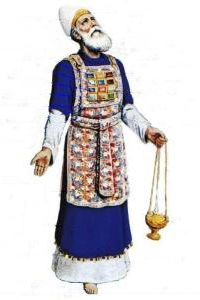
\includegraphics[width=50mm,scale=1.5]{Melchisedec.jpg}
\vspace{0.4in}

% Create a title for the document and write it in bold font
\LARGE{\textbf{\date}}
\linebreak

\vspace{0.5in}


\begin{flushleft}
\LARGE{1 Samuel\\}\vspace{0.25in}
\LARGE{Notes, Outlines, Comments}
\end{flushleft}

% write in large letters
%\large{Free webservices and apps}

% Skip some space
\vspace{0.6in}

%\large{Documentation}
% Skip some space

\bigskip

\normalsize{Xenia, Oh.\\}
\normalsize{created: \today}

% Skip some space
\vspace{1.3in}

\end{flushright}
% End the title page
\end{titlepage}

%\titlehttps://www.overleaf.com/project/60d732302fc633866943c9d2JE

\newpage 

\tableofcontents\hypertarget{TOC}{}
\listoffigures
\listoftables

\hyphenation{A-bim-e-lech bre-thren E-phra-im  Gib-e-o-nites Jer-u-sa-lem through-out Phil-i-stines The-o-phil-us Am-a-le-kites ven-geance Mesh-el-e-mi-ah onan-ism Phar-a-oh Py-thon thoughts grev-ous-ness Hach-a-liah adul-ter-er Shad-rach}

%\fcolorbox{black}{bone}{TEXT}
%%%%%%%%%%%%%%%%% EXTRA COLORS
%%%%%%%%%%%%%%%%% EXTRA COLORS
%%%%%%%%%%%%%%%%% EXTRA COLORS
\definecolor{champagne}{rgb}{0.97,0.91,0.81}
\definecolor{bone}{rgb}{0.89,0.85,0.79}

\definecolor{ForestGreen}{rgb}{0.00,0.29,0.098}
\definecolor{GIVING}{cmyk}{1,0.0,0.72,.1}

\definecolor{MLPE}{cmyk}{1,1,0,.45}
\definecolor{SOCCER}{cmyk}{.77, 0, .42, .49}
\definecolor{PAYBILL}{cmyk}{0,0.83,0.76,0.07}
\definecolor{SERMON}{cmyk}{.14,.9,0,.30} % aka seance \href{http://www.flatuicolorpicker.com/purple-cmyk-color-model/}{seance}
\definecolor{BIBLE}{cmyk}{0,.17,.74,.17}
\definecolor{WORKBLUE}{cmyk}{1, .5, 0, .6}
\definecolor{myOrange}{cmyk}{0, .4, .98, .03}
\definecolor{myTan}{cmyk}{0.0,.07,.17,.10}
\definecolor{myRed}{cmyk}{0,1,1,0}
\definecolor{myWhite}{cmyk}{0,0,0,0}
\definecolor{BLUESoD}{cmyk}{.97,.84,0,.04}
\definecolor{WHITE}{cmyk}{0,0,0,0}
\definecolor{OLDGOLD}{cmyk}{0.05,0.3,1.00,0}
\definecolor{CASTLETON}{cmyk}{1,0,0.31,0.66}
\definecolor{cadmiumgreen}{rgb}{0.0, 0.42, 0.24}
\definecolor{jungle}{rgb}{0.203,0.4882,0.1718}
\definecolor{MYGOLD}{rgb}{1,.84,0}

\definecolor{MYLIGHTGRAY}{rgb}{.85,.85,.85}

\definecolor{codegreen}{rgb}{0,0.6,0}
\definecolor{codegray}{rgb}{0.5,0.5,0.5}
\definecolor{codepurple}{rgb}{0.58,0,0.82}
\definecolor{backcolour}{rgb}{0.95,0.95,0.92}



\mdfdefinestyle{MyFrame}{%
    linecolor=blue,
    outerlinewidth=2pt,
    roundcorner=5pt,
    innertopmargin=\baselineskip,
    innerbottommargin=\baselineskip,
    innerrightmargin=10pt,
    innerleftmargin=10pt,
    backgroundcolor=gray!25!white}


\mdfdefinestyle{MyFrame2}{%
    linecolor=black,
    outerlinewidth=2pt,
    roundcorner=5pt,
    innertopmargin=\baselineskip,
    innerbottommargin=\baselineskip,
    innerrightmargin=10pt,
    innerleftmargin=10pt,
    backgroundcolor=yellow!25!white}



%\input{PFTTIS}
%\input{WFTTIS}
%\input{WFITV}


\chapter{1 Samuel 1}

\begin{figure}
  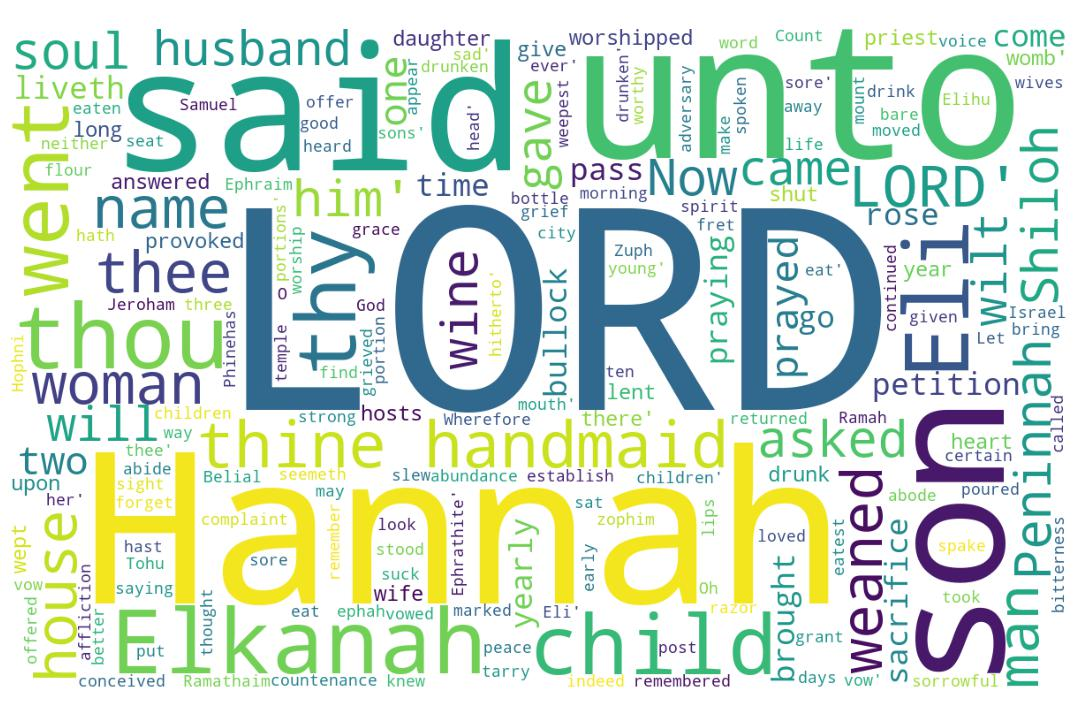
\includegraphics[width=\linewidth]{09OT-1Samuel/1Samuel1-WordCloud.jpg}
  \caption{1 Samuel 1 Word Cloud}
  \label{fig:1 Samuel 1 Word Cloud}
\end{figure}

\marginpar{\scriptsize \centering \fcolorbox{bone}{lime}{\textbf{A LENT SON}}\\ (1 Samuel 1:1-28) \begin{compactenum}[I.][8]
    \item A \textbf{Barren Woman}  \index[scripture]{1Samuel!1Sa 01:05}(1Sa 1:5)
    \item \textbf{Bitter \& Weeping}  \index[scripture]{1Samuel!1Sa 01:10}(1Sa 1:10)
    \item \textbf{Belial's Women}  \index[scripture]{1Samuel!1Sa 01:16}(1Sa 1:16)
    \item A \textbf{Baby Awaited}  \index[scripture]{1Samuel!1Sa 01:18}(1Sa 1:18)
    \item The \textbf{Boy Weaned}  \index[scripture]{1Samuel!1Sa 01:23}(1Sa 1:23)
    \item A \textbf{Blessed Woman}  \index[scripture]{1Samuel!1Sa 01:27}(1Sa 1:27)
    \item A \textbf{Boy Worshipping}  \index[scripture]{1Samuel!1Sa 01:28}(1Sa 1:28)
\end{compactenum}}






\footnote{\textcolor[cmyk]{0.99998,1,0,0}{\hyperlink{TOC}{Return to end of Table of Contents.}}}\footnote{\href{https://audiobible.com/bible/1_samuel_1.html}{\textcolor[cmyk]{0.99998,1,0,0}{1 Samuel 1 Audio}}}\textcolor[cmyk]{0.99998,1,0,0}{Now there was a certain man of Ramathaim-zophim, of mount Ephraim, and his name \emph{was} Elkanah, the son of Jeroham, the son of Elihu, the son of Tohu, the son of Zuph, an Ephrathite:}
[2] \textcolor[cmyk]{0.99998,1,0,0}{And he had two wives; the name of the one \emph{was} Hannah, and the name of the other Peninnah: and Peninnah had children, but Hannah had no children.}
[3] \textcolor[cmyk]{0.99998,1,0,0}{And this man went up out of his city yearly to worship and to sacrifice unto the LORD of hosts in Shiloh. And the two sons of Eli, Hophni and Phinehas, the priests of the LORD, \emph{were} there.}\\
\\
\P \textcolor[cmyk]{0.99998,1,0,0}{And when the time was that Elkanah offered, he gave to Peninnah his wife, and to all her sons and her daughters, portions:}
[5] \textcolor[cmyk]{0.99998,1,0,0}{But unto Hannah he gave a worthy portion; for he loved Hannah: but the LORD had \fcolorbox{bone}{lime}{shut up her womb}.}
[6] \textcolor[cmyk]{0.99998,1,0,0}{And her adversary also provoked her sore, for to make her fret, because the LORD had shut up her womb.}
[7] \textcolor[cmyk]{0.99998,1,0,0}{And \emph{as} he did so year by year, when she went up to the house of the LORD, so she provoked her; therefore she wept, and did not eat.}
[8] \textcolor[cmyk]{0.99998,1,0,0}{Then said Elkanah her husband to her, Hannah, why weepest thou? and why eatest thou not? and why is thy heart grieved? \emph{am} not I better to thee than ten sons?}\\
\\
\P \textcolor[cmyk]{0.99998,1,0,0}{So Hannah rose up after they had eaten in Shiloh, and after they had drunk. Now Eli the priest sat upon a seat by a post of the temple of the LORD.}
[10] \textcolor[cmyk]{0.99998,1,0,0}{And she \emph{was} \fcolorbox{bone}{lime}{in bitterness} of soul, and prayed unto the LORD, and wept sore.}
[11] \textcolor[cmyk]{0.99998,1,0,0}{And she vowed a vow, and said, O LORD of hosts, if thou wilt indeed look on the affliction of thine handmaid, and remember me, and not forget thine handmaid, but wilt give unto thine handmaid a man child, then I will give him unto the LORD all the days of his life, and there shall no razor come upon his head.}
[12] \textcolor[cmyk]{0.99998,1,0,0}{And it came to pass, as she continued praying before the LORD, that Eli marked her mouth.}
[13] \textcolor[cmyk]{0.99998,1,0,0}{Now Hannah, she spake in her heart; only her lips moved, but her voice was not heard: therefore Eli thought she had been drunken.}
[14] \textcolor[cmyk]{0.99998,1,0,0}{And Eli said unto her, How long wilt thou be drunken? put away thy wine from thee.}
[15] \textcolor[cmyk]{0.99998,1,0,0}{And Hannah answered and said, No, my lord, I \emph{am} a woman of a sorrowful spirit: I have drunk neither wine nor strong drink, but have poured out my soul before the LORD.}
[16] \textcolor[cmyk]{0.99998,1,0,0}{Count not thine handmaid for a \fcolorbox{bone}{lime}{daughter of Belial}: for out of the abundance of my complaint and grief have I spoken hitherto.}
[17] \textcolor[cmyk]{0.99998,1,0,0}{Then Eli answered and said, Go in peace: and the God of Israel grant \emph{thee} thy petition that thou hast asked of him.}
[18] \textcolor[cmyk]{0.99998,1,0,0}{And she said, Let thine handmaid find grace in thy sight. So the woman went her way, and did eat, and her countenance was no more \emph{sad}.}\\
\\
\P \textcolor[cmyk]{0.99998,1,0,0}{And they rose up in the morning early, and worshipped before the LORD, and returned, and came to their house to Ramah: and Elkanah knew Hannah his wife; and the LORD remembered her.}
[20] \textcolor[cmyk]{0.99998,1,0,0}{Wherefore it came to pass, when the time was come about after Hannah had conceived, that she bare a son, and called his name Samuel, \emph{saying}, Because I have asked him of the LORD.}
[21] \textcolor[cmyk]{0.99998,1,0,0}{And the man Elkanah, and all his house, went up to offer unto the LORD the yearly sacrifice, and his vow.}
[22] \textcolor[cmyk]{0.99998,1,0,0}{But Hannah went not up; for she said unto her husband, \emph{I} \emph{will} \emph{not} \emph{go} \emph{up} until the child be weaned, and \emph{then} I will bring him, that he may appear before the LORD, and there abide for ever.}
[23] \textcolor[cmyk]{0.99998,1,0,0}{And Elkanah her husband said unto her, Do what seemeth thee good; tarry until thou have \fcolorbox{bone}{lime}{weaned} him; only the LORD establish his word. So the woman abode, and gave her son suck until she \fcolorbox{bone}{lime}{weaned} him.}\\
\\
\P \textcolor[cmyk]{0.99998,1,0,0}{And when she had weaned him, she took him up with her, with three bullocks, and one ephah of flour, and a bottle of wine, and brought him unto the house of the LORD in Shiloh: and the child \emph{was} young.}
[25] \textcolor[cmyk]{0.99998,1,0,0}{And they slew a bullock, and brought the child to Eli.}
[26] \textcolor[cmyk]{0.99998,1,0,0}{And she said, Oh my lord, \emph{as} thy soul liveth, my lord, I \emph{am} the woman that stood by thee here, praying unto the LORD.}
[27] \textcolor[cmyk]{0.99998,1,0,0}{For this child I prayed; and the \fcolorbox{bone}{lime}{LORD hath given me} my petition which I asked of him:}
[28] \textcolor[cmyk]{0.99998,1,0,0}{Therefore also I have lent him to the LORD; as long as he liveth he shall be lent to the LORD. And \fcolorbox{bone}{lime}{he worshipped} the LORD there.}
\section{1 Samuel 1 Comments}


%\index[NWIV]{34!1Samuel!1Sa 1:1}\index[AWIP]{Now!1Samuel!1Sa 1:1}\index[AWIP]{there!1Samuel!1Sa 1:1}\index[AWIP]{was!1Samuel!1Sa 1:1}\index[AWIP]{a!1Samuel!1Sa 1:1}\index[AWIP]{certain!1Samuel!1Sa 1:1}\index[AWIP]{man!1Samuel!1Sa 1:1}\index[AWIP]{of!1Samuel!1Sa 1:1}\index[AWIP]{of!1Samuel!1Sa 1:1 (2)}\index[AWIP]{of!1Samuel!1Sa 1:1 (3)}\index[AWIP]{of!1Samuel!1Sa 1:1 (4)}\index[AWIP]{of!1Samuel!1Sa 1:1 (5)}\index[AWIP]{of!1Samuel!1Sa 1:1 (6)}\index[AWIP]{Ramathaim-zophim!1Samuel!1Sa 1:1}\index[AWIP]{mount!1Samuel!1Sa 1:1}\index[AWIP]{Ephraim!1Samuel!1Sa 1:1}\index[AWIP]{and!1Samuel!1Sa 1:1}\index[AWIP]{his!1Samuel!1Sa 1:1}\index[AWIP]{name!1Samuel!1Sa 1:1}\index[AWIP]{\emph{was}!1Samuel!1Sa 1:1}\index[AWIP]{Elkanah!1Samuel!1Sa 1:1}\index[AWIP]{the!1Samuel!1Sa 1:1}\index[AWIP]{the!1Samuel!1Sa 1:1 (2)}\index[AWIP]{the!1Samuel!1Sa 1:1 (3)}\index[AWIP]{the!1Samuel!1Sa 1:1 (4)}\index[AWIP]{son!1Samuel!1Sa 1:1}\index[AWIP]{son!1Samuel!1Sa 1:1 (2)}\index[AWIP]{son!1Samuel!1Sa 1:1 (3)}\index[AWIP]{son!1Samuel!1Sa 1:1 (4)}\index[AWIP]{Jeroham!1Samuel!1Sa 1:1}\index[AWIP]{Elihu!1Samuel!1Sa 1:1}\index[AWIP]{Tohu!1Samuel!1Sa 1:1}\index[AWIP]{Zuph!1Samuel!1Sa 1:1}\index[AWIP]{an!1Samuel!1Sa 1:1}\index[AWIP]{Ephrathite!1Samuel!1Sa 1:1}\index[AWIP]{\emph{was}!1Samuel!1Sa 1:1}

\index[NWIV]{28!1Samuel!1Sa 1:2}\index[AWIP]{And!1Samuel!1Sa 1:2}\index[AWIP]{he!1Samuel!1Sa 1:2}\index[AWIP]{had!1Samuel!1Sa 1:2}\index[AWIP]{had!1Samuel!1Sa 1:2 (2)}\index[AWIP]{had!1Samuel!1Sa 1:2 (3)}\index[AWIP]{two!1Samuel!1Sa 1:2}\index[AWIP]{wives!1Samuel!1Sa 1:2}\index[AWIP]{the!1Samuel!1Sa 1:2}\index[AWIP]{the!1Samuel!1Sa 1:2 (2)}\index[AWIP]{the!1Samuel!1Sa 1:2 (3)}\index[AWIP]{the!1Samuel!1Sa 1:2 (4)}\index[AWIP]{name!1Samuel!1Sa 1:2}\index[AWIP]{name!1Samuel!1Sa 1:2 (2)}\index[AWIP]{of!1Samuel!1Sa 1:2}\index[AWIP]{of!1Samuel!1Sa 1:2 (2)}\index[AWIP]{one!1Samuel!1Sa 1:2}\index[AWIP]{\emph{was}!1Samuel!1Sa 1:2}\index[AWIP]{Hannah!1Samuel!1Sa 1:2}\index[AWIP]{Hannah!1Samuel!1Sa 1:2 (2)}\index[AWIP]{and!1Samuel!1Sa 1:2}\index[AWIP]{and!1Samuel!1Sa 1:2 (2)}\index[AWIP]{other!1Samuel!1Sa 1:2}\index[AWIP]{Peninnah!1Samuel!1Sa 1:2}\index[AWIP]{Peninnah!1Samuel!1Sa 1:2 (2)}\index[AWIP]{children!1Samuel!1Sa 1:2}\index[AWIP]{children!1Samuel!1Sa 1:2 (2)}\index[AWIP]{but!1Samuel!1Sa 1:2}\index[AWIP]{no!1Samuel!1Sa 1:2}\index[AWIP]{\emph{was}!1Samuel!1Sa 1:2}

\index[NWIV]{38!1Samuel!1Sa 1:3}\index[AWIP]{And!1Samuel!1Sa 1:3}\index[AWIP]{And!1Samuel!1Sa 1:3 (2)}\index[AWIP]{this!1Samuel!1Sa 1:3}\index[AWIP]{man!1Samuel!1Sa 1:3}\index[AWIP]{went!1Samuel!1Sa 1:3}\index[AWIP]{up!1Samuel!1Sa 1:3}\index[AWIP]{out!1Samuel!1Sa 1:3}\index[AWIP]{of!1Samuel!1Sa 1:3}\index[AWIP]{of!1Samuel!1Sa 1:3 (2)}\index[AWIP]{of!1Samuel!1Sa 1:3 (3)}\index[AWIP]{of!1Samuel!1Sa 1:3 (4)}\index[AWIP]{his!1Samuel!1Sa 1:3}\index[AWIP]{city!1Samuel!1Sa 1:3}\index[AWIP]{yearly!1Samuel!1Sa 1:3}\index[AWIP]{to!1Samuel!1Sa 1:3}\index[AWIP]{to!1Samuel!1Sa 1:3 (2)}\index[AWIP]{worship!1Samuel!1Sa 1:3}\index[AWIP]{and!1Samuel!1Sa 1:3}\index[AWIP]{and!1Samuel!1Sa 1:3 (2)}\index[AWIP]{sacrifice!1Samuel!1Sa 1:3}\index[AWIP]{unto!1Samuel!1Sa 1:3}\index[AWIP]{the!1Samuel!1Sa 1:3}\index[AWIP]{the!1Samuel!1Sa 1:3 (2)}\index[AWIP]{the!1Samuel!1Sa 1:3 (3)}\index[AWIP]{the!1Samuel!1Sa 1:3 (4)}\index[AWIP]{LORD!1Samuel!1Sa 1:3}\index[AWIP]{LORD!1Samuel!1Sa 1:3 (2)}\index[AWIP]{hosts!1Samuel!1Sa 1:3}\index[AWIP]{in!1Samuel!1Sa 1:3}\index[AWIP]{Shiloh!1Samuel!1Sa 1:3}\index[AWIP]{two!1Samuel!1Sa 1:3}\index[AWIP]{sons!1Samuel!1Sa 1:3}\index[AWIP]{Eli!1Samuel!1Sa 1:3}\index[AWIP]{Hophni!1Samuel!1Sa 1:3}\index[AWIP]{Phinehas!1Samuel!1Sa 1:3}\index[AWIP]{priests!1Samuel!1Sa 1:3}\index[AWIP]{\emph{were}!1Samuel!1Sa 1:3}\index[AWIP]{there!1Samuel!1Sa 1:3}\index[AWIP]{\emph{were}!1Samuel!1Sa 1:3}

\index[NWIV]{23!1Samuel!1Sa 1:4}\index[AWIP]{And!1Samuel!1Sa 1:4}\index[AWIP]{when!1Samuel!1Sa 1:4}\index[AWIP]{the!1Samuel!1Sa 1:4}\index[AWIP]{time!1Samuel!1Sa 1:4}\index[AWIP]{was!1Samuel!1Sa 1:4}\index[AWIP]{that!1Samuel!1Sa 1:4}\index[AWIP]{Elkanah!1Samuel!1Sa 1:4}\index[AWIP]{offered!1Samuel!1Sa 1:4}\index[AWIP]{he!1Samuel!1Sa 1:4}\index[AWIP]{gave!1Samuel!1Sa 1:4}\index[AWIP]{to!1Samuel!1Sa 1:4}\index[AWIP]{to!1Samuel!1Sa 1:4 (2)}\index[AWIP]{Peninnah!1Samuel!1Sa 1:4}\index[AWIP]{his!1Samuel!1Sa 1:4}\index[AWIP]{wife!1Samuel!1Sa 1:4}\index[AWIP]{and!1Samuel!1Sa 1:4}\index[AWIP]{and!1Samuel!1Sa 1:4 (2)}\index[AWIP]{all!1Samuel!1Sa 1:4}\index[AWIP]{her!1Samuel!1Sa 1:4}\index[AWIP]{her!1Samuel!1Sa 1:4 (2)}\index[AWIP]{sons!1Samuel!1Sa 1:4}\index[AWIP]{daughters!1Samuel!1Sa 1:4}\index[AWIP]{portions!1Samuel!1Sa 1:4}

\index[NWIV]{20!1Samuel!1Sa 1:5}\index[AWIP]{But!1Samuel!1Sa 1:5}\index[AWIP]{unto!1Samuel!1Sa 1:5}\index[AWIP]{Hannah!1Samuel!1Sa 1:5}\index[AWIP]{Hannah!1Samuel!1Sa 1:5 (2)}\index[AWIP]{he!1Samuel!1Sa 1:5}\index[AWIP]{he!1Samuel!1Sa 1:5 (2)}\index[AWIP]{gave!1Samuel!1Sa 1:5}\index[AWIP]{a!1Samuel!1Sa 1:5}\index[AWIP]{worthy!1Samuel!1Sa 1:5}\index[AWIP]{portion!1Samuel!1Sa 1:5}\index[AWIP]{for!1Samuel!1Sa 1:5}\index[AWIP]{loved!1Samuel!1Sa 1:5}\index[AWIP]{but!1Samuel!1Sa 1:5}\index[AWIP]{the!1Samuel!1Sa 1:5}\index[AWIP]{LORD!1Samuel!1Sa 1:5}\index[AWIP]{had!1Samuel!1Sa 1:5}\index[AWIP]{shut!1Samuel!1Sa 1:5}\index[AWIP]{up!1Samuel!1Sa 1:5}\index[AWIP]{her!1Samuel!1Sa 1:5}\index[AWIP]{womb!1Samuel!1Sa 1:5}

\index[NWIV]{20!1Samuel!1Sa 1:6}\index[AWIP]{And!1Samuel!1Sa 1:6}\index[AWIP]{her!1Samuel!1Sa 1:6}\index[AWIP]{her!1Samuel!1Sa 1:6 (2)}\index[AWIP]{her!1Samuel!1Sa 1:6 (3)}\index[AWIP]{her!1Samuel!1Sa 1:6 (4)}\index[AWIP]{adversary!1Samuel!1Sa 1:6}\index[AWIP]{also!1Samuel!1Sa 1:6}\index[AWIP]{provoked!1Samuel!1Sa 1:6}\index[AWIP]{sore!1Samuel!1Sa 1:6}\index[AWIP]{for!1Samuel!1Sa 1:6}\index[AWIP]{to!1Samuel!1Sa 1:6}\index[AWIP]{make!1Samuel!1Sa 1:6}\index[AWIP]{fret!1Samuel!1Sa 1:6}\index[AWIP]{because!1Samuel!1Sa 1:6}\index[AWIP]{the!1Samuel!1Sa 1:6}\index[AWIP]{LORD!1Samuel!1Sa 1:6}\index[AWIP]{had!1Samuel!1Sa 1:6}\index[AWIP]{shut!1Samuel!1Sa 1:6}\index[AWIP]{up!1Samuel!1Sa 1:6}\index[AWIP]{womb!1Samuel!1Sa 1:6}

\index[NWIV]{29!1Samuel!1Sa 1:7}\index[AWIP]{And!1Samuel!1Sa 1:7}\index[AWIP]{\emph{as}!1Samuel!1Sa 1:7}\index[AWIP]{he!1Samuel!1Sa 1:7}\index[AWIP]{did!1Samuel!1Sa 1:7}\index[AWIP]{did!1Samuel!1Sa 1:7 (2)}\index[AWIP]{so!1Samuel!1Sa 1:7}\index[AWIP]{so!1Samuel!1Sa 1:7 (2)}\index[AWIP]{year!1Samuel!1Sa 1:7}\index[AWIP]{year!1Samuel!1Sa 1:7 (2)}\index[AWIP]{by!1Samuel!1Sa 1:7}\index[AWIP]{when!1Samuel!1Sa 1:7}\index[AWIP]{she!1Samuel!1Sa 1:7}\index[AWIP]{she!1Samuel!1Sa 1:7 (2)}\index[AWIP]{she!1Samuel!1Sa 1:7 (3)}\index[AWIP]{went!1Samuel!1Sa 1:7}\index[AWIP]{up!1Samuel!1Sa 1:7}\index[AWIP]{to!1Samuel!1Sa 1:7}\index[AWIP]{the!1Samuel!1Sa 1:7}\index[AWIP]{the!1Samuel!1Sa 1:7 (2)}\index[AWIP]{house!1Samuel!1Sa 1:7}\index[AWIP]{of!1Samuel!1Sa 1:7}\index[AWIP]{LORD!1Samuel!1Sa 1:7}\index[AWIP]{provoked!1Samuel!1Sa 1:7}\index[AWIP]{her!1Samuel!1Sa 1:7}\index[AWIP]{therefore!1Samuel!1Sa 1:7}\index[AWIP]{wept!1Samuel!1Sa 1:7}\index[AWIP]{and!1Samuel!1Sa 1:7}\index[AWIP]{not!1Samuel!1Sa 1:7}\index[AWIP]{eat!1Samuel!1Sa 1:7}\index[AWIP]{\emph{as}!1Samuel!1Sa 1:7}

\index[NWIV]{31!1Samuel!1Sa 1:8}\index[AWIP]{Then!1Samuel!1Sa 1:8}\index[AWIP]{said!1Samuel!1Sa 1:8}\index[AWIP]{Elkanah!1Samuel!1Sa 1:8}\index[AWIP]{her!1Samuel!1Sa 1:8}\index[AWIP]{her!1Samuel!1Sa 1:8 (2)}\index[AWIP]{husband!1Samuel!1Sa 1:8}\index[AWIP]{to!1Samuel!1Sa 1:8}\index[AWIP]{to!1Samuel!1Sa 1:8 (2)}\index[AWIP]{Hannah!1Samuel!1Sa 1:8}\index[AWIP]{why!1Samuel!1Sa 1:8}\index[AWIP]{why!1Samuel!1Sa 1:8 (2)}\index[AWIP]{why!1Samuel!1Sa 1:8 (3)}\index[AWIP]{weepest!1Samuel!1Sa 1:8}\index[AWIP]{thou?!1Samuel!1Sa 1:8}\index[AWIP]{and!1Samuel!1Sa 1:8}\index[AWIP]{and!1Samuel!1Sa 1:8 (2)}\index[AWIP]{eatest!1Samuel!1Sa 1:8}\index[AWIP]{thou!1Samuel!1Sa 1:8}\index[AWIP]{not?!1Samuel!1Sa 1:8}\index[AWIP]{is!1Samuel!1Sa 1:8}\index[AWIP]{thy!1Samuel!1Sa 1:8}\index[AWIP]{heart!1Samuel!1Sa 1:8}\index[AWIP]{grieved?!1Samuel!1Sa 1:8}\index[AWIP]{\emph{am}!1Samuel!1Sa 1:8}\index[AWIP]{not!1Samuel!1Sa 1:8}\index[AWIP]{I!1Samuel!1Sa 1:8}\index[AWIP]{better!1Samuel!1Sa 1:8}\index[AWIP]{thee!1Samuel!1Sa 1:8}\index[AWIP]{than!1Samuel!1Sa 1:8}\index[AWIP]{ten!1Samuel!1Sa 1:8}\index[AWIP]{sons?!1Samuel!1Sa 1:8}\index[AWIP]{\emph{am}!1Samuel!1Sa 1:8}

\index[NWIV]{32!1Samuel!1Sa 1:9}\index[AWIP]{So!1Samuel!1Sa 1:9}\index[AWIP]{Hannah!1Samuel!1Sa 1:9}\index[AWIP]{rose!1Samuel!1Sa 1:9}\index[AWIP]{up!1Samuel!1Sa 1:9}\index[AWIP]{after!1Samuel!1Sa 1:9}\index[AWIP]{after!1Samuel!1Sa 1:9 (2)}\index[AWIP]{they!1Samuel!1Sa 1:9}\index[AWIP]{they!1Samuel!1Sa 1:9 (2)}\index[AWIP]{had!1Samuel!1Sa 1:9}\index[AWIP]{had!1Samuel!1Sa 1:9 (2)}\index[AWIP]{eaten!1Samuel!1Sa 1:9}\index[AWIP]{in!1Samuel!1Sa 1:9}\index[AWIP]{Shiloh!1Samuel!1Sa 1:9}\index[AWIP]{and!1Samuel!1Sa 1:9}\index[AWIP]{drunk!1Samuel!1Sa 1:9}\index[AWIP]{Now!1Samuel!1Sa 1:9}\index[AWIP]{Eli!1Samuel!1Sa 1:9}\index[AWIP]{the!1Samuel!1Sa 1:9}\index[AWIP]{the!1Samuel!1Sa 1:9 (2)}\index[AWIP]{the!1Samuel!1Sa 1:9 (3)}\index[AWIP]{priest!1Samuel!1Sa 1:9}\index[AWIP]{sat!1Samuel!1Sa 1:9}\index[AWIP]{upon!1Samuel!1Sa 1:9}\index[AWIP]{a!1Samuel!1Sa 1:9}\index[AWIP]{a!1Samuel!1Sa 1:9 (2)}\index[AWIP]{seat!1Samuel!1Sa 1:9}\index[AWIP]{by!1Samuel!1Sa 1:9}\index[AWIP]{post!1Samuel!1Sa 1:9}\index[AWIP]{of!1Samuel!1Sa 1:9}\index[AWIP]{of!1Samuel!1Sa 1:9 (2)}\index[AWIP]{temple!1Samuel!1Sa 1:9}\index[AWIP]{LORD!1Samuel!1Sa 1:9}

\index[NWIV]{15!1Samuel!1Sa 1:10}\index[AWIP]{And!1Samuel!1Sa 1:10}\index[AWIP]{she!1Samuel!1Sa 1:10}\index[AWIP]{\emph{was}!1Samuel!1Sa 1:10}\index[AWIP]{in!1Samuel!1Sa 1:10}\index[AWIP]{bitterness!1Samuel!1Sa 1:10}\index[AWIP]{of!1Samuel!1Sa 1:10}\index[AWIP]{soul!1Samuel!1Sa 1:10}\index[AWIP]{and!1Samuel!1Sa 1:10}\index[AWIP]{and!1Samuel!1Sa 1:10 (2)}\index[AWIP]{prayed!1Samuel!1Sa 1:10}\index[AWIP]{unto!1Samuel!1Sa 1:10}\index[AWIP]{the!1Samuel!1Sa 1:10}\index[AWIP]{LORD!1Samuel!1Sa 1:10}\index[AWIP]{wept!1Samuel!1Sa 1:10}\index[AWIP]{sore!1Samuel!1Sa 1:10}\index[AWIP]{\emph{was}!1Samuel!1Sa 1:10}

\index[NWIV]{62!1Samuel!1Sa 1:11}\index[AWIP]{And!1Samuel!1Sa 1:11}\index[AWIP]{she!1Samuel!1Sa 1:11}\index[AWIP]{vowed!1Samuel!1Sa 1:11}\index[AWIP]{a!1Samuel!1Sa 1:11}\index[AWIP]{a!1Samuel!1Sa 1:11 (2)}\index[AWIP]{vow!1Samuel!1Sa 1:11}\index[AWIP]{and!1Samuel!1Sa 1:11}\index[AWIP]{and!1Samuel!1Sa 1:11 (2)}\index[AWIP]{and!1Samuel!1Sa 1:11 (3)}\index[AWIP]{and!1Samuel!1Sa 1:11 (4)}\index[AWIP]{said!1Samuel!1Sa 1:11}\index[AWIP]{O!1Samuel!1Sa 1:11}\index[AWIP]{LORD!1Samuel!1Sa 1:11}\index[AWIP]{LORD!1Samuel!1Sa 1:11 (2)}\index[AWIP]{of!1Samuel!1Sa 1:11}\index[AWIP]{of!1Samuel!1Sa 1:11 (2)}\index[AWIP]{of!1Samuel!1Sa 1:11 (3)}\index[AWIP]{hosts!1Samuel!1Sa 1:11}\index[AWIP]{if!1Samuel!1Sa 1:11}\index[AWIP]{thou!1Samuel!1Sa 1:11}\index[AWIP]{wilt!1Samuel!1Sa 1:11}\index[AWIP]{wilt!1Samuel!1Sa 1:11 (2)}\index[AWIP]{indeed!1Samuel!1Sa 1:11}\index[AWIP]{look!1Samuel!1Sa 1:11}\index[AWIP]{on!1Samuel!1Sa 1:11}\index[AWIP]{the!1Samuel!1Sa 1:11}\index[AWIP]{the!1Samuel!1Sa 1:11 (2)}\index[AWIP]{the!1Samuel!1Sa 1:11 (3)}\index[AWIP]{affliction!1Samuel!1Sa 1:11}\index[AWIP]{thine!1Samuel!1Sa 1:11}\index[AWIP]{thine!1Samuel!1Sa 1:11 (2)}\index[AWIP]{thine!1Samuel!1Sa 1:11 (3)}\index[AWIP]{handmaid!1Samuel!1Sa 1:11}\index[AWIP]{handmaid!1Samuel!1Sa 1:11 (2)}\index[AWIP]{handmaid!1Samuel!1Sa 1:11 (3)}\index[AWIP]{remember!1Samuel!1Sa 1:11}\index[AWIP]{me!1Samuel!1Sa 1:11}\index[AWIP]{not!1Samuel!1Sa 1:11}\index[AWIP]{forget!1Samuel!1Sa 1:11}\index[AWIP]{but!1Samuel!1Sa 1:11}\index[AWIP]{give!1Samuel!1Sa 1:11}\index[AWIP]{give!1Samuel!1Sa 1:11 (2)}\index[AWIP]{unto!1Samuel!1Sa 1:11}\index[AWIP]{unto!1Samuel!1Sa 1:11 (2)}\index[AWIP]{man!1Samuel!1Sa 1:11}\index[AWIP]{child!1Samuel!1Sa 1:11}\index[AWIP]{then!1Samuel!1Sa 1:11}\index[AWIP]{I!1Samuel!1Sa 1:11}\index[AWIP]{will!1Samuel!1Sa 1:11}\index[AWIP]{him!1Samuel!1Sa 1:11}\index[AWIP]{all!1Samuel!1Sa 1:11}\index[AWIP]{days!1Samuel!1Sa 1:11}\index[AWIP]{his!1Samuel!1Sa 1:11}\index[AWIP]{his!1Samuel!1Sa 1:11 (2)}\index[AWIP]{life!1Samuel!1Sa 1:11}\index[AWIP]{there!1Samuel!1Sa 1:11}\index[AWIP]{shall!1Samuel!1Sa 1:11}\index[AWIP]{no!1Samuel!1Sa 1:11}\index[AWIP]{razor!1Samuel!1Sa 1:11}\index[AWIP]{come!1Samuel!1Sa 1:11}\index[AWIP]{upon!1Samuel!1Sa 1:11}\index[AWIP]{head!1Samuel!1Sa 1:11}

\index[NWIV]{17!1Samuel!1Sa 1:12}\index[AWIP]{And!1Samuel!1Sa 1:12}\index[AWIP]{it!1Samuel!1Sa 1:12}\index[AWIP]{came!1Samuel!1Sa 1:12}\index[AWIP]{to!1Samuel!1Sa 1:12}\index[AWIP]{pass!1Samuel!1Sa 1:12}\index[AWIP]{as!1Samuel!1Sa 1:12}\index[AWIP]{she!1Samuel!1Sa 1:12}\index[AWIP]{continued!1Samuel!1Sa 1:12}\index[AWIP]{praying!1Samuel!1Sa 1:12}\index[AWIP]{before!1Samuel!1Sa 1:12}\index[AWIP]{the!1Samuel!1Sa 1:12}\index[AWIP]{LORD!1Samuel!1Sa 1:12}\index[AWIP]{that!1Samuel!1Sa 1:12}\index[AWIP]{Eli!1Samuel!1Sa 1:12}\index[AWIP]{marked!1Samuel!1Sa 1:12}\index[AWIP]{her!1Samuel!1Sa 1:12}\index[AWIP]{mouth!1Samuel!1Sa 1:12}

\index[NWIV]{24!1Samuel!1Sa 1:13}\index[AWIP]{Now!1Samuel!1Sa 1:13}\index[AWIP]{Hannah!1Samuel!1Sa 1:13}\index[AWIP]{she!1Samuel!1Sa 1:13}\index[AWIP]{she!1Samuel!1Sa 1:13 (2)}\index[AWIP]{spake!1Samuel!1Sa 1:13}\index[AWIP]{in!1Samuel!1Sa 1:13}\index[AWIP]{her!1Samuel!1Sa 1:13}\index[AWIP]{her!1Samuel!1Sa 1:13 (2)}\index[AWIP]{her!1Samuel!1Sa 1:13 (3)}\index[AWIP]{heart!1Samuel!1Sa 1:13}\index[AWIP]{only!1Samuel!1Sa 1:13}\index[AWIP]{lips!1Samuel!1Sa 1:13}\index[AWIP]{moved!1Samuel!1Sa 1:13}\index[AWIP]{but!1Samuel!1Sa 1:13}\index[AWIP]{voice!1Samuel!1Sa 1:13}\index[AWIP]{was!1Samuel!1Sa 1:13}\index[AWIP]{not!1Samuel!1Sa 1:13}\index[AWIP]{heard!1Samuel!1Sa 1:13}\index[AWIP]{therefore!1Samuel!1Sa 1:13}\index[AWIP]{Eli!1Samuel!1Sa 1:13}\index[AWIP]{thought!1Samuel!1Sa 1:13}\index[AWIP]{had!1Samuel!1Sa 1:13}\index[AWIP]{been!1Samuel!1Sa 1:13}\index[AWIP]{drunken!1Samuel!1Sa 1:13}

\index[NWIV]{17!1Samuel!1Sa 1:14}\index[AWIP]{And!1Samuel!1Sa 1:14}\index[AWIP]{Eli!1Samuel!1Sa 1:14}\index[AWIP]{said!1Samuel!1Sa 1:14}\index[AWIP]{unto!1Samuel!1Sa 1:14}\index[AWIP]{her!1Samuel!1Sa 1:14}\index[AWIP]{How!1Samuel!1Sa 1:14}\index[AWIP]{long!1Samuel!1Sa 1:14}\index[AWIP]{wilt!1Samuel!1Sa 1:14}\index[AWIP]{thou!1Samuel!1Sa 1:14}\index[AWIP]{be!1Samuel!1Sa 1:14}\index[AWIP]{drunken?!1Samuel!1Sa 1:14}\index[AWIP]{put!1Samuel!1Sa 1:14}\index[AWIP]{away!1Samuel!1Sa 1:14}\index[AWIP]{thy!1Samuel!1Sa 1:14}\index[AWIP]{wine!1Samuel!1Sa 1:14}\index[AWIP]{from!1Samuel!1Sa 1:14}\index[AWIP]{thee!1Samuel!1Sa 1:14}

\index[NWIV]{33!1Samuel!1Sa 1:15}\index[AWIP]{And!1Samuel!1Sa 1:15}\index[AWIP]{Hannah!1Samuel!1Sa 1:15}\index[AWIP]{answered!1Samuel!1Sa 1:15}\index[AWIP]{and!1Samuel!1Sa 1:15}\index[AWIP]{said!1Samuel!1Sa 1:15}\index[AWIP]{No!1Samuel!1Sa 1:15}\index[AWIP]{my!1Samuel!1Sa 1:15}\index[AWIP]{my!1Samuel!1Sa 1:15 (2)}\index[AWIP]{lord!1Samuel!1Sa 1:15}\index[AWIP]{I!1Samuel!1Sa 1:15}\index[AWIP]{I!1Samuel!1Sa 1:15 (2)}\index[AWIP]{\emph{am}!1Samuel!1Sa 1:15}\index[AWIP]{a!1Samuel!1Sa 1:15}\index[AWIP]{a!1Samuel!1Sa 1:15 (2)}\index[AWIP]{woman!1Samuel!1Sa 1:15}\index[AWIP]{of!1Samuel!1Sa 1:15}\index[AWIP]{sorrowful!1Samuel!1Sa 1:15}\index[AWIP]{spirit!1Samuel!1Sa 1:15}\index[AWIP]{have!1Samuel!1Sa 1:15}\index[AWIP]{have!1Samuel!1Sa 1:15 (2)}\index[AWIP]{drunk!1Samuel!1Sa 1:15}\index[AWIP]{neither!1Samuel!1Sa 1:15}\index[AWIP]{wine!1Samuel!1Sa 1:15}\index[AWIP]{nor!1Samuel!1Sa 1:15}\index[AWIP]{strong!1Samuel!1Sa 1:15}\index[AWIP]{drink!1Samuel!1Sa 1:15}\index[AWIP]{but!1Samuel!1Sa 1:15}\index[AWIP]{poured!1Samuel!1Sa 1:15}\index[AWIP]{out!1Samuel!1Sa 1:15}\index[AWIP]{soul!1Samuel!1Sa 1:15}\index[AWIP]{before!1Samuel!1Sa 1:15}\index[AWIP]{the!1Samuel!1Sa 1:15}\index[AWIP]{LORD!1Samuel!1Sa 1:15}\index[AWIP]{\emph{am}!1Samuel!1Sa 1:15}

\index[NWIV]{23!1Samuel!1Sa 1:16}\index[AWIP]{Count!1Samuel!1Sa 1:16}\index[AWIP]{not!1Samuel!1Sa 1:16}\index[AWIP]{thine!1Samuel!1Sa 1:16}\index[AWIP]{handmaid!1Samuel!1Sa 1:16}\index[AWIP]{for!1Samuel!1Sa 1:16}\index[AWIP]{for!1Samuel!1Sa 1:16 (2)}\index[AWIP]{a!1Samuel!1Sa 1:16}\index[AWIP]{daughter!1Samuel!1Sa 1:16}\index[AWIP]{of!1Samuel!1Sa 1:16}\index[AWIP]{of!1Samuel!1Sa 1:16 (2)}\index[AWIP]{of!1Samuel!1Sa 1:16 (3)}\index[AWIP]{Belial!1Samuel!1Sa 1:16}\index[AWIP]{out!1Samuel!1Sa 1:16}\index[AWIP]{the!1Samuel!1Sa 1:16}\index[AWIP]{abundance!1Samuel!1Sa 1:16}\index[AWIP]{my!1Samuel!1Sa 1:16}\index[AWIP]{complaint!1Samuel!1Sa 1:16}\index[AWIP]{and!1Samuel!1Sa 1:16}\index[AWIP]{grief!1Samuel!1Sa 1:16}\index[AWIP]{have!1Samuel!1Sa 1:16}\index[AWIP]{I!1Samuel!1Sa 1:16}\index[AWIP]{spoken!1Samuel!1Sa 1:16}\index[AWIP]{hitherto!1Samuel!1Sa 1:16}

\index[NWIV]{23!1Samuel!1Sa 1:17}\index[AWIP]{Then!1Samuel!1Sa 1:17}\index[AWIP]{Eli!1Samuel!1Sa 1:17}\index[AWIP]{answered!1Samuel!1Sa 1:17}\index[AWIP]{and!1Samuel!1Sa 1:17}\index[AWIP]{and!1Samuel!1Sa 1:17 (2)}\index[AWIP]{said!1Samuel!1Sa 1:17}\index[AWIP]{Go!1Samuel!1Sa 1:17}\index[AWIP]{in!1Samuel!1Sa 1:17}\index[AWIP]{peace!1Samuel!1Sa 1:17}\index[AWIP]{the!1Samuel!1Sa 1:17}\index[AWIP]{God!1Samuel!1Sa 1:17}\index[AWIP]{of!1Samuel!1Sa 1:17}\index[AWIP]{of!1Samuel!1Sa 1:17 (2)}\index[AWIP]{Israel!1Samuel!1Sa 1:17}\index[AWIP]{grant!1Samuel!1Sa 1:17}\index[AWIP]{\emph{thee}!1Samuel!1Sa 1:17}\index[AWIP]{thy!1Samuel!1Sa 1:17}\index[AWIP]{petition!1Samuel!1Sa 1:17}\index[AWIP]{that!1Samuel!1Sa 1:17}\index[AWIP]{thou!1Samuel!1Sa 1:17}\index[AWIP]{hast!1Samuel!1Sa 1:17}\index[AWIP]{asked!1Samuel!1Sa 1:17}\index[AWIP]{him!1Samuel!1Sa 1:17}\index[AWIP]{\emph{thee}!1Samuel!1Sa 1:17}

\index[NWIV]{27!1Samuel!1Sa 1:18}\index[AWIP]{And!1Samuel!1Sa 1:18}\index[AWIP]{she!1Samuel!1Sa 1:18}\index[AWIP]{said!1Samuel!1Sa 1:18}\index[AWIP]{Let!1Samuel!1Sa 1:18}\index[AWIP]{thine!1Samuel!1Sa 1:18}\index[AWIP]{handmaid!1Samuel!1Sa 1:18}\index[AWIP]{find!1Samuel!1Sa 1:18}\index[AWIP]{grace!1Samuel!1Sa 1:18}\index[AWIP]{in!1Samuel!1Sa 1:18}\index[AWIP]{thy!1Samuel!1Sa 1:18}\index[AWIP]{sight!1Samuel!1Sa 1:18}\index[AWIP]{So!1Samuel!1Sa 1:18}\index[AWIP]{the!1Samuel!1Sa 1:18}\index[AWIP]{woman!1Samuel!1Sa 1:18}\index[AWIP]{went!1Samuel!1Sa 1:18}\index[AWIP]{her!1Samuel!1Sa 1:18}\index[AWIP]{her!1Samuel!1Sa 1:18 (2)}\index[AWIP]{way!1Samuel!1Sa 1:18}\index[AWIP]{and!1Samuel!1Sa 1:18}\index[AWIP]{and!1Samuel!1Sa 1:18 (2)}\index[AWIP]{did!1Samuel!1Sa 1:18}\index[AWIP]{eat!1Samuel!1Sa 1:18}\index[AWIP]{countenance!1Samuel!1Sa 1:18}\index[AWIP]{was!1Samuel!1Sa 1:18}\index[AWIP]{no!1Samuel!1Sa 1:18}\index[AWIP]{more!1Samuel!1Sa 1:18}\index[AWIP]{\emph{sad}!1Samuel!1Sa 1:18}\index[AWIP]{\emph{sad}!1Samuel!1Sa 1:18}

\index[NWIV]{33!1Samuel!1Sa 1:19}\index[AWIP]{And!1Samuel!1Sa 1:19}\index[AWIP]{they!1Samuel!1Sa 1:19}\index[AWIP]{rose!1Samuel!1Sa 1:19}\index[AWIP]{up!1Samuel!1Sa 1:19}\index[AWIP]{in!1Samuel!1Sa 1:19}\index[AWIP]{the!1Samuel!1Sa 1:19}\index[AWIP]{the!1Samuel!1Sa 1:19 (2)}\index[AWIP]{the!1Samuel!1Sa 1:19 (3)}\index[AWIP]{morning!1Samuel!1Sa 1:19}\index[AWIP]{early!1Samuel!1Sa 1:19}\index[AWIP]{and!1Samuel!1Sa 1:19}\index[AWIP]{and!1Samuel!1Sa 1:19 (2)}\index[AWIP]{and!1Samuel!1Sa 1:19 (3)}\index[AWIP]{and!1Samuel!1Sa 1:19 (4)}\index[AWIP]{and!1Samuel!1Sa 1:19 (5)}\index[AWIP]{worshipped!1Samuel!1Sa 1:19}\index[AWIP]{before!1Samuel!1Sa 1:19}\index[AWIP]{LORD!1Samuel!1Sa 1:19}\index[AWIP]{LORD!1Samuel!1Sa 1:19 (2)}\index[AWIP]{returned!1Samuel!1Sa 1:19}\index[AWIP]{came!1Samuel!1Sa 1:19}\index[AWIP]{to!1Samuel!1Sa 1:19}\index[AWIP]{to!1Samuel!1Sa 1:19 (2)}\index[AWIP]{their!1Samuel!1Sa 1:19}\index[AWIP]{house!1Samuel!1Sa 1:19}\index[AWIP]{Ramah!1Samuel!1Sa 1:19}\index[AWIP]{Elkanah!1Samuel!1Sa 1:19}\index[AWIP]{knew!1Samuel!1Sa 1:19}\index[AWIP]{Hannah!1Samuel!1Sa 1:19}\index[AWIP]{his!1Samuel!1Sa 1:19}\index[AWIP]{wife!1Samuel!1Sa 1:19}\index[AWIP]{remembered!1Samuel!1Sa 1:19}\index[AWIP]{her!1Samuel!1Sa 1:19}

\index[NWIV]{34!1Samuel!1Sa 1:20}\index[AWIP]{Wherefore!1Samuel!1Sa 1:20}\index[AWIP]{it!1Samuel!1Sa 1:20}\index[AWIP]{came!1Samuel!1Sa 1:20}\index[AWIP]{to!1Samuel!1Sa 1:20}\index[AWIP]{pass!1Samuel!1Sa 1:20}\index[AWIP]{when!1Samuel!1Sa 1:20}\index[AWIP]{the!1Samuel!1Sa 1:20}\index[AWIP]{the!1Samuel!1Sa 1:20 (2)}\index[AWIP]{time!1Samuel!1Sa 1:20}\index[AWIP]{was!1Samuel!1Sa 1:20}\index[AWIP]{come!1Samuel!1Sa 1:20}\index[AWIP]{about!1Samuel!1Sa 1:20}\index[AWIP]{after!1Samuel!1Sa 1:20}\index[AWIP]{Hannah!1Samuel!1Sa 1:20}\index[AWIP]{had!1Samuel!1Sa 1:20}\index[AWIP]{conceived!1Samuel!1Sa 1:20}\index[AWIP]{that!1Samuel!1Sa 1:20}\index[AWIP]{she!1Samuel!1Sa 1:20}\index[AWIP]{bare!1Samuel!1Sa 1:20}\index[AWIP]{a!1Samuel!1Sa 1:20}\index[AWIP]{son!1Samuel!1Sa 1:20}\index[AWIP]{and!1Samuel!1Sa 1:20}\index[AWIP]{called!1Samuel!1Sa 1:20}\index[AWIP]{his!1Samuel!1Sa 1:20}\index[AWIP]{name!1Samuel!1Sa 1:20}\index[AWIP]{Samuel!1Samuel!1Sa 1:20}\index[AWIP]{\emph{saying}!1Samuel!1Sa 1:20}\index[AWIP]{Because!1Samuel!1Sa 1:20}\index[AWIP]{I!1Samuel!1Sa 1:20}\index[AWIP]{have!1Samuel!1Sa 1:20}\index[AWIP]{asked!1Samuel!1Sa 1:20}\index[AWIP]{him!1Samuel!1Sa 1:20}\index[AWIP]{of!1Samuel!1Sa 1:20}\index[AWIP]{LORD!1Samuel!1Sa 1:20}\index[AWIP]{\emph{saying}!1Samuel!1Sa 1:20}

\index[NWIV]{21!1Samuel!1Sa 1:21}\index[AWIP]{And!1Samuel!1Sa 1:21}\index[AWIP]{the!1Samuel!1Sa 1:21}\index[AWIP]{the!1Samuel!1Sa 1:21 (2)}\index[AWIP]{the!1Samuel!1Sa 1:21 (3)}\index[AWIP]{man!1Samuel!1Sa 1:21}\index[AWIP]{Elkanah!1Samuel!1Sa 1:21}\index[AWIP]{and!1Samuel!1Sa 1:21}\index[AWIP]{and!1Samuel!1Sa 1:21 (2)}\index[AWIP]{all!1Samuel!1Sa 1:21}\index[AWIP]{his!1Samuel!1Sa 1:21}\index[AWIP]{his!1Samuel!1Sa 1:21 (2)}\index[AWIP]{house!1Samuel!1Sa 1:21}\index[AWIP]{went!1Samuel!1Sa 1:21}\index[AWIP]{up!1Samuel!1Sa 1:21}\index[AWIP]{to!1Samuel!1Sa 1:21}\index[AWIP]{offer!1Samuel!1Sa 1:21}\index[AWIP]{unto!1Samuel!1Sa 1:21}\index[AWIP]{LORD!1Samuel!1Sa 1:21}\index[AWIP]{yearly!1Samuel!1Sa 1:21}\index[AWIP]{sacrifice!1Samuel!1Sa 1:21}\index[AWIP]{vow!1Samuel!1Sa 1:21}

\index[NWIV]{39!1Samuel!1Sa 1:22}\index[AWIP]{But!1Samuel!1Sa 1:22}\index[AWIP]{Hannah!1Samuel!1Sa 1:22}\index[AWIP]{went!1Samuel!1Sa 1:22}\index[AWIP]{not!1Samuel!1Sa 1:22}\index[AWIP]{up!1Samuel!1Sa 1:22}\index[AWIP]{for!1Samuel!1Sa 1:22}\index[AWIP]{for!1Samuel!1Sa 1:22 (2)}\index[AWIP]{she!1Samuel!1Sa 1:22}\index[AWIP]{said!1Samuel!1Sa 1:22}\index[AWIP]{unto!1Samuel!1Sa 1:22}\index[AWIP]{her!1Samuel!1Sa 1:22}\index[AWIP]{husband!1Samuel!1Sa 1:22}\index[AWIP]{\emph{I}!1Samuel!1Sa 1:22}\index[AWIP]{\emph{will}!1Samuel!1Sa 1:22}\index[AWIP]{\emph{not}!1Samuel!1Sa 1:22}\index[AWIP]{\emph{go}!1Samuel!1Sa 1:22}\index[AWIP]{\emph{up}!1Samuel!1Sa 1:22}\index[AWIP]{until!1Samuel!1Sa 1:22}\index[AWIP]{the!1Samuel!1Sa 1:22}\index[AWIP]{the!1Samuel!1Sa 1:22 (2)}\index[AWIP]{child!1Samuel!1Sa 1:22}\index[AWIP]{be!1Samuel!1Sa 1:22}\index[AWIP]{weaned!1Samuel!1Sa 1:22}\index[AWIP]{and!1Samuel!1Sa 1:22}\index[AWIP]{and!1Samuel!1Sa 1:22 (2)}\index[AWIP]{\emph{then}!1Samuel!1Sa 1:22}\index[AWIP]{I!1Samuel!1Sa 1:22}\index[AWIP]{will!1Samuel!1Sa 1:22}\index[AWIP]{bring!1Samuel!1Sa 1:22}\index[AWIP]{him!1Samuel!1Sa 1:22}\index[AWIP]{that!1Samuel!1Sa 1:22}\index[AWIP]{he!1Samuel!1Sa 1:22}\index[AWIP]{may!1Samuel!1Sa 1:22}\index[AWIP]{appear!1Samuel!1Sa 1:22}\index[AWIP]{before!1Samuel!1Sa 1:22}\index[AWIP]{LORD!1Samuel!1Sa 1:22}\index[AWIP]{there!1Samuel!1Sa 1:22}\index[AWIP]{abide!1Samuel!1Sa 1:22}\index[AWIP]{ever!1Samuel!1Sa 1:22}\index[AWIP]{\emph{I}!1Samuel!1Sa 1:22}\index[AWIP]{\emph{will}!1Samuel!1Sa 1:22}\index[AWIP]{\emph{not}!1Samuel!1Sa 1:22}\index[AWIP]{\emph{go}!1Samuel!1Sa 1:22}\index[AWIP]{\emph{up}!1Samuel!1Sa 1:22}\index[AWIP]{\emph{then}!1Samuel!1Sa 1:22}

\index[NWIV]{37!1Samuel!1Sa 1:23}\index[AWIP]{And!1Samuel!1Sa 1:23}\index[AWIP]{Elkanah!1Samuel!1Sa 1:23}\index[AWIP]{her!1Samuel!1Sa 1:23}\index[AWIP]{her!1Samuel!1Sa 1:23 (2)}\index[AWIP]{her!1Samuel!1Sa 1:23 (3)}\index[AWIP]{husband!1Samuel!1Sa 1:23}\index[AWIP]{said!1Samuel!1Sa 1:23}\index[AWIP]{unto!1Samuel!1Sa 1:23}\index[AWIP]{Do!1Samuel!1Sa 1:23}\index[AWIP]{what!1Samuel!1Sa 1:23}\index[AWIP]{seemeth!1Samuel!1Sa 1:23}\index[AWIP]{thee!1Samuel!1Sa 1:23}\index[AWIP]{good!1Samuel!1Sa 1:23}\index[AWIP]{tarry!1Samuel!1Sa 1:23}\index[AWIP]{until!1Samuel!1Sa 1:23}\index[AWIP]{until!1Samuel!1Sa 1:23 (2)}\index[AWIP]{thou!1Samuel!1Sa 1:23}\index[AWIP]{have!1Samuel!1Sa 1:23}\index[AWIP]{weaned!1Samuel!1Sa 1:23}\index[AWIP]{weaned!1Samuel!1Sa 1:23 (2)}\index[AWIP]{him!1Samuel!1Sa 1:23}\index[AWIP]{him!1Samuel!1Sa 1:23 (2)}\index[AWIP]{only!1Samuel!1Sa 1:23}\index[AWIP]{the!1Samuel!1Sa 1:23}\index[AWIP]{the!1Samuel!1Sa 1:23 (2)}\index[AWIP]{LORD!1Samuel!1Sa 1:23}\index[AWIP]{establish!1Samuel!1Sa 1:23}\index[AWIP]{his!1Samuel!1Sa 1:23}\index[AWIP]{word!1Samuel!1Sa 1:23}\index[AWIP]{So!1Samuel!1Sa 1:23}\index[AWIP]{woman!1Samuel!1Sa 1:23}\index[AWIP]{abode!1Samuel!1Sa 1:23}\index[AWIP]{and!1Samuel!1Sa 1:23}\index[AWIP]{gave!1Samuel!1Sa 1:23}\index[AWIP]{son!1Samuel!1Sa 1:23}\index[AWIP]{suck!1Samuel!1Sa 1:23}\index[AWIP]{she!1Samuel!1Sa 1:23}

\index[NWIV]{41!1Samuel!1Sa 1:24}\index[AWIP]{And!1Samuel!1Sa 1:24}\index[AWIP]{when!1Samuel!1Sa 1:24}\index[AWIP]{she!1Samuel!1Sa 1:24}\index[AWIP]{she!1Samuel!1Sa 1:24 (2)}\index[AWIP]{had!1Samuel!1Sa 1:24}\index[AWIP]{weaned!1Samuel!1Sa 1:24}\index[AWIP]{him!1Samuel!1Sa 1:24}\index[AWIP]{him!1Samuel!1Sa 1:24 (2)}\index[AWIP]{him!1Samuel!1Sa 1:24 (3)}\index[AWIP]{took!1Samuel!1Sa 1:24}\index[AWIP]{up!1Samuel!1Sa 1:24}\index[AWIP]{with!1Samuel!1Sa 1:24}\index[AWIP]{with!1Samuel!1Sa 1:24 (2)}\index[AWIP]{her!1Samuel!1Sa 1:24}\index[AWIP]{three!1Samuel!1Sa 1:24}\index[AWIP]{bullocks!1Samuel!1Sa 1:24}\index[AWIP]{and!1Samuel!1Sa 1:24}\index[AWIP]{and!1Samuel!1Sa 1:24 (2)}\index[AWIP]{and!1Samuel!1Sa 1:24 (3)}\index[AWIP]{and!1Samuel!1Sa 1:24 (4)}\index[AWIP]{one!1Samuel!1Sa 1:24}\index[AWIP]{ephah!1Samuel!1Sa 1:24}\index[AWIP]{of!1Samuel!1Sa 1:24}\index[AWIP]{of!1Samuel!1Sa 1:24 (2)}\index[AWIP]{of!1Samuel!1Sa 1:24 (3)}\index[AWIP]{flour!1Samuel!1Sa 1:24}\index[AWIP]{a!1Samuel!1Sa 1:24}\index[AWIP]{bottle!1Samuel!1Sa 1:24}\index[AWIP]{wine!1Samuel!1Sa 1:24}\index[AWIP]{brought!1Samuel!1Sa 1:24}\index[AWIP]{unto!1Samuel!1Sa 1:24}\index[AWIP]{the!1Samuel!1Sa 1:24}\index[AWIP]{the!1Samuel!1Sa 1:24 (2)}\index[AWIP]{the!1Samuel!1Sa 1:24 (3)}\index[AWIP]{house!1Samuel!1Sa 1:24}\index[AWIP]{LORD!1Samuel!1Sa 1:24}\index[AWIP]{in!1Samuel!1Sa 1:24}\index[AWIP]{Shiloh!1Samuel!1Sa 1:24}\index[AWIP]{child!1Samuel!1Sa 1:24}\index[AWIP]{\emph{was}!1Samuel!1Sa 1:24}\index[AWIP]{young!1Samuel!1Sa 1:24}\index[AWIP]{\emph{was}!1Samuel!1Sa 1:24}

\index[NWIV]{11!1Samuel!1Sa 1:25}\index[AWIP]{And!1Samuel!1Sa 1:25}\index[AWIP]{they!1Samuel!1Sa 1:25}\index[AWIP]{slew!1Samuel!1Sa 1:25}\index[AWIP]{a!1Samuel!1Sa 1:25}\index[AWIP]{bullock!1Samuel!1Sa 1:25}\index[AWIP]{and!1Samuel!1Sa 1:25}\index[AWIP]{brought!1Samuel!1Sa 1:25}\index[AWIP]{the!1Samuel!1Sa 1:25}\index[AWIP]{child!1Samuel!1Sa 1:25}\index[AWIP]{to!1Samuel!1Sa 1:25}\index[AWIP]{Eli!1Samuel!1Sa 1:25}

\index[NWIV]{25!1Samuel!1Sa 1:26}\index[AWIP]{And!1Samuel!1Sa 1:26}\index[AWIP]{she!1Samuel!1Sa 1:26}\index[AWIP]{said!1Samuel!1Sa 1:26}\index[AWIP]{Oh!1Samuel!1Sa 1:26}\index[AWIP]{my!1Samuel!1Sa 1:26}\index[AWIP]{my!1Samuel!1Sa 1:26 (2)}\index[AWIP]{lord!1Samuel!1Sa 1:26}\index[AWIP]{lord!1Samuel!1Sa 1:26 (2)}\index[AWIP]{\emph{as}!1Samuel!1Sa 1:26}\index[AWIP]{thy!1Samuel!1Sa 1:26}\index[AWIP]{soul!1Samuel!1Sa 1:26}\index[AWIP]{liveth!1Samuel!1Sa 1:26}\index[AWIP]{I!1Samuel!1Sa 1:26}\index[AWIP]{\emph{am}!1Samuel!1Sa 1:26}\index[AWIP]{the!1Samuel!1Sa 1:26}\index[AWIP]{the!1Samuel!1Sa 1:26 (2)}\index[AWIP]{woman!1Samuel!1Sa 1:26}\index[AWIP]{that!1Samuel!1Sa 1:26}\index[AWIP]{stood!1Samuel!1Sa 1:26}\index[AWIP]{by!1Samuel!1Sa 1:26}\index[AWIP]{thee!1Samuel!1Sa 1:26}\index[AWIP]{here!1Samuel!1Sa 1:26}\index[AWIP]{praying!1Samuel!1Sa 1:26}\index[AWIP]{unto!1Samuel!1Sa 1:26}\index[AWIP]{LORD!1Samuel!1Sa 1:26}\index[AWIP]{\emph{as}!1Samuel!1Sa 1:26}\index[AWIP]{\emph{am}!1Samuel!1Sa 1:26}

\index[NWIV]{18!1Samuel!1Sa 1:27}\index[AWIP]{For!1Samuel!1Sa 1:27}\index[AWIP]{this!1Samuel!1Sa 1:27}\index[AWIP]{child!1Samuel!1Sa 1:27}\index[AWIP]{I!1Samuel!1Sa 1:27}\index[AWIP]{I!1Samuel!1Sa 1:27 (2)}\index[AWIP]{prayed!1Samuel!1Sa 1:27}\index[AWIP]{and!1Samuel!1Sa 1:27}\index[AWIP]{the!1Samuel!1Sa 1:27}\index[AWIP]{LORD!1Samuel!1Sa 1:27}\index[AWIP]{hath!1Samuel!1Sa 1:27}\index[AWIP]{given!1Samuel!1Sa 1:27}\index[AWIP]{me!1Samuel!1Sa 1:27}\index[AWIP]{my!1Samuel!1Sa 1:27}\index[AWIP]{petition!1Samuel!1Sa 1:27}\index[AWIP]{which!1Samuel!1Sa 1:27}\index[AWIP]{asked!1Samuel!1Sa 1:27}\index[AWIP]{of!1Samuel!1Sa 1:27}\index[AWIP]{him!1Samuel!1Sa 1:27}

\index[NWIV]{27!1Samuel!1Sa 1:28}\index[AWIP]{Therefore!1Samuel!1Sa 1:28}\index[AWIP]{also!1Samuel!1Sa 1:28}\index[AWIP]{I!1Samuel!1Sa 1:28}\index[AWIP]{have!1Samuel!1Sa 1:28}\index[AWIP]{lent!1Samuel!1Sa 1:28}\index[AWIP]{lent!1Samuel!1Sa 1:28 (2)}\index[AWIP]{him!1Samuel!1Sa 1:28}\index[AWIP]{to!1Samuel!1Sa 1:28}\index[AWIP]{to!1Samuel!1Sa 1:28 (2)}\index[AWIP]{the!1Samuel!1Sa 1:28}\index[AWIP]{the!1Samuel!1Sa 1:28 (2)}\index[AWIP]{the!1Samuel!1Sa 1:28 (3)}\index[AWIP]{LORD!1Samuel!1Sa 1:28}\index[AWIP]{LORD!1Samuel!1Sa 1:28 (2)}\index[AWIP]{LORD!1Samuel!1Sa 1:28 (3)}\index[AWIP]{as!1Samuel!1Sa 1:28}\index[AWIP]{as!1Samuel!1Sa 1:28 (2)}\index[AWIP]{long!1Samuel!1Sa 1:28}\index[AWIP]{he!1Samuel!1Sa 1:28}\index[AWIP]{he!1Samuel!1Sa 1:28 (2)}\index[AWIP]{he!1Samuel!1Sa 1:28 (3)}\index[AWIP]{liveth!1Samuel!1Sa 1:28}\index[AWIP]{shall!1Samuel!1Sa 1:28}\index[AWIP]{be!1Samuel!1Sa 1:28}\index[AWIP]{And!1Samuel!1Sa 1:28}\index[AWIP]{worshipped!1Samuel!1Sa 1:28}\index[AWIP]{there!1Samuel!1Sa 1:28}


\section{1 Samuel 1 Outlines}

\subsection{My Outlines}

\subsubsection{A Lent Son}
\index[speaker]{Keith Anthony!1 Samuel 01 (A Lent Son)}
\index[series]{1 Samuel (Keith Anthony)!1 Samuel 01 (A Lent Son)}
\index[date]{2019/03/24!1 Samuel 01 (A Lent Son) (Keith Anthony)}

\begin{compactenum}[I.][7]
    \item A \textbf{Barren Woman}  \index[scripture]{1Samuel!1Sa 01:05}(1Sa 1:5)
    \item \textbf{Bitter \& Weeping}  \index[scripture]{1Samuel!1Sa 01:10}(1Sa 1:10)
    \item \textbf{Belial's Women}  \index[scripture]{1Samuel!1Sa 01:16}(1Sa 1:16)
    \item A \textbf{Baby Awaited}  \index[scripture]{1Samuel!1Sa 01:18}(1Sa 1:18)
    \item The \textbf{Boy Weaned}  \index[scripture]{1Samuel!1Sa 01:23}(1Sa 1:23)
    \item A \textbf{Blessed Woman}  \index[scripture]{1Samuel!1Sa 01:27}(1Sa 1:27)
    \item A \textbf{Boy Worshipping}  \index[scripture]{1Samuel!1Sa 01:28}(1Sa 1:28)
\end{compactenum}



\subsection{My Outlines from Others}

\subsubsection{A Son for Hannah}
\index[speaker]{Matt Bernsdorff!1 Samuel 01 (Samuel: A Yearning Heart \& A Baby’s Cry)}
\index[series]{1 Samuel (Matt Bernsdorff)!1 Samuel 01 (Samuel: A Yearning Heart \& A Baby’s Cry)}
\index[date]{unknown!1 Samuel 01 (Samuel: A Yearning Heart \& A Baby’s Cry) (Matt Bernsdorff)}
\textbf{Source: } Highlights Sunday School Curriculum
\begin{compactenum}[I.][7]
    \item The \textbf{Priest}  \index[scripture]{1Samuel!1Sa 01:03}(1Sa 1:3)
    \item A \textbf{Preference}  \index[scripture]{1Samuel!1Sa 01:05}(1Sa 1:5)
    \item The \textbf{Provocation} \index[scripture]{1Samuel!1Sa 01:06} \index[scripture]{1Samuel!1Sa 01:07}  (1Sa 1:6, 7)
    \item The \textbf{Passion} \index[scripture]{1Samuel!1Sa 01:07}(1Sa 1:7)
    \item The \textbf{Petition} \index[scripture]{1Samuel!1Sa 01:11}(1Sa 1:11
    \item The \textbf{Promise} \index[scripture]{1Samuel!1Sa 01:17}(1Sa 1:17)
    \item The \textbf{Presentation} \index[scripture]{1Samuel!1Sa 01:28}(1Sa 1:28)
\end{compactenum}

\subsubsection{God Answers Prayer}
\index[speaker]{Warren Wiersbe!1 Samuel 01 (God Answers Prayer)}
\index[series]{1 Samuel (Warren Wiersbe)!1 Samuel 01 (God Answers Prayer)}
\index[date]{unknown!1 Samuel 01 (God Answers Prayer) (Warren Wiersbe)}
\textbf{Source: }Wiersbe, BE Successful, Commentary on 1 Samuel
\begin{compactenum}[I.][7]
    \item A \textbf{Divided Home}  \index[scripture]{1Samuel!1Sa 01:01--08}(1Sa 1:1--8)
    \item A \textbf{Devout Prayer}  \index[scripture]{1Samuel!1Sa 01:09--19}(1Sa 1:9--18)
    \item A \textbf{Distinguished Son}  \index[scripture]{1Samuel!1Sa 01:19--28}(1Sa 1:19--28)
\end{compactenum}

%\\section{1 Samuel 1 Statistics}

%%%%%%%%%%%%%%%%%%%%%%%%%%%
%%%%% Word Statistics
%%%%%%%%%%%%%%%%%%%%%%%%%%


\normalsize



\subsection{Chapter Word Statistics}


%%%%%%%%%%
%%%%%%%%%%
 
\begin{center}
\begin{longtable}{l|c|c|c|c}
\caption[Stats for FirstSamuel 1]{Stats for FirstSamuel 1} \label{table:Stats for FirstSamuel 1} \\ 
\hline \multicolumn{1}{|c|}{\textbf{Verse(s)}} & \multicolumn{1}{|c|}{\textbf{Count}} & \multicolumn{1}{|c|}{\textbf{Unique}} & \multicolumn{1}{|c|}{\textbf{Italics}} & \multicolumn{1}{|c|}{\textbf{Uniq Italic}}  \\ \hline 
\endfirsthead
 
\multicolumn{5}{c}
{{\bfseries \tablename\ \thetable{} -- continued from previous page}} \\  
\hline \multicolumn{1}{|c|}{\textbf{Verse(s)}} & \multicolumn{1}{|c|}{\textbf{Count}} & \multicolumn{1}{|c|}{\textbf{Unique}} & \multicolumn{1}{|c|}{\textbf{Italics}} & \multicolumn{1}{|c|}{\textbf{Uniq Italic}}  \\ \hline 
\endhead
 
\hline \multicolumn{5}{|r|}{{Continued if needed}} \\ \hline
\endfoot 
1 & 34 & 23 & 1 & 1\\ \hline
2 & 28 & 17 & 1 & 1\\ \hline
3 & 38 & 28 & 1 & 1\\ \hline
4 & 23 & 20 & 0 & 0\\ \hline
5 & 20 & 18 & 0 & 0\\ \hline
6 & 20 & 17 & 0 & 0\\ \hline
7 & 29 & 23 & 1 & 1\\ \hline
8 & 31 & 24 & 1 & 1\\ \hline
9 & 32 & 25 & 0 & 0\\ \hline
10 & 15 & 14 & 1 & 1\\ \hline
11 & 62 & 45 & 0 & 0\\ \hline
12 & 17 & 17 & 0 & 0\\ \hline
13 & 24 & 21 & 0 & 0\\ \hline
14 & 17 & 17 & 0 & 0\\ \hline
15 & 33 & 29 & 1 & 1\\ \hline
16 & 23 & 20 & 0 & 0\\ \hline
17 & 23 & 21 & 1 & 1\\ \hline
18 & 27 & 25 & 1 & 1\\ \hline
19 & 33 & 25 & 0 & 0\\ \hline
20 & 34 & 33 & 1 & 1\\ \hline
21 & 21 & 17 & 0 & 0\\ \hline
22 & 39 & 36 & 6 & 6\\ \hline
23 & 37 & 31 & 0 & 0\\ \hline
24 & 41 & 30 & 1 & 1\\ \hline
25 & 11 & 11 & 0 & 0\\ \hline
26 & 25 & 22 & 2 & 2\\ \hline
27 & 18 & 17 & 0 & 0\\ \hline
28 & 27 & 18 & 0 & 0\\ \hline
\hline \hline
Total & 782 & 270 & 19 & 13



\end{longtable}
\end{center}

%%%%%%%%%%
%%%%%%%%%%
 
\subsection{Words by Frequency}

\begin{center}
\begin{longtable}{l|r}
\caption[Word Frequencies in FirstSamuel 1]{Word Frequencies in FirstSamuel 1} \label{table:WordsIn-FirstSamuel-1} \\ 
\hline \multicolumn{1}{|c|}{\textbf{Word}} & \multicolumn{1}{c|}{\textbf{Frequency}} \\ \hline 
\endfirsthead
 
\multicolumn{2}{c}
{{\bfseries \tablename\ \thetable{} -- continued from previous page}} \\ 
\hline \multicolumn{1}{|c|}{\textbf{Word}} & \multicolumn{1}{c|}{\textbf{Frequency}} \\ \hline 
\endhead
 
\hline \multicolumn{2}{|r|}{{Continued if needed}} \\ \hline
\endfoot
 
\hline \hline
\endlastfoot
the & 51 \\ \hline
and & 40 \\ \hline
of & 30 \\ \hline
LORD & 23 \\ \hline
her & 23 \\ \hline
And & 19 \\ \hline
to & 16 \\ \hline
she & 15 \\ \hline
a & 12 \\ \hline
Hannah & 11 \\ \hline
unto & 11 \\ \hline
I & 11 \\ \hline
him & 11 \\ \hline
his & 10 \\ \hline
had & 10 \\ \hline
he & 9 \\ \hline
up & 9 \\ \hline
said & 9 \\ \hline
in & 8 \\ \hline
Eli & 7 \\ \hline
not & 7 \\ \hline
Elkanah & 6 \\ \hline
son & 6 \\ \hline
that & 6 \\ \hline
for & 6 \\ \hline
thou & 6 \\ \hline
my & 6 \\ \hline
have & 6 \\ \hline
there & 5 \\ \hline
was & 5 \\ \hline
but & 5 \\ \hline
went & 5 \\ \hline
thy & 5 \\ \hline
thine & 5 \\ \hline
handmaid & 5 \\ \hline
child & 5 \\ \hline
man & 4 \\ \hline
name & 4 \\ \hline
\emph{was} & 4 \\ \hline
when & 4 \\ \hline
house & 4 \\ \hline
thee & 4 \\ \hline
they & 4 \\ \hline
before & 4 \\ \hline
woman & 4 \\ \hline
weaned & 4 \\ \hline
Now & 3 \\ \hline
Peninnah & 3 \\ \hline
no & 3 \\ \hline
out & 3 \\ \hline
Shiloh & 3 \\ \hline
sons & 3 \\ \hline
gave & 3 \\ \hline
all & 3 \\ \hline
did & 3 \\ \hline
by & 3 \\ \hline
husband & 3 \\ \hline
why & 3 \\ \hline
\emph{am} & 3 \\ \hline
So & 3 \\ \hline
after & 3 \\ \hline
soul & 3 \\ \hline
wilt & 3 \\ \hline
came & 3 \\ \hline
as & 3 \\ \hline
be & 3 \\ \hline
wine & 3 \\ \hline
lord & 3 \\ \hline
asked & 3 \\ \hline
until & 3 \\ \hline
two & 2 \\ \hline
one & 2 \\ \hline
children & 2 \\ \hline
this & 2 \\ \hline
yearly & 2 \\ \hline
sacrifice & 2 \\ \hline
hosts & 2 \\ \hline
time & 2 \\ \hline
wife & 2 \\ \hline
But & 2 \\ \hline
shut & 2 \\ \hline
womb & 2 \\ \hline
also & 2 \\ \hline
provoked & 2 \\ \hline
sore & 2 \\ \hline
\emph{as} & 2 \\ \hline
so & 2 \\ \hline
year & 2 \\ \hline
therefore & 2 \\ \hline
wept & 2 \\ \hline
eat & 2 \\ \hline
Then & 2 \\ \hline
heart & 2 \\ \hline
rose & 2 \\ \hline
drunk & 2 \\ \hline
upon & 2 \\ \hline
prayed & 2 \\ \hline
vow & 2 \\ \hline
me & 2 \\ \hline
give & 2 \\ \hline
will & 2 \\ \hline
shall & 2 \\ \hline
come & 2 \\ \hline
it & 2 \\ \hline
pass & 2 \\ \hline
praying & 2 \\ \hline
only & 2 \\ \hline
drunken & 2 \\ \hline
long & 2 \\ \hline
answered & 2 \\ \hline
petition & 2 \\ \hline
worshipped & 2 \\ \hline
with & 2 \\ \hline
brought & 2 \\ \hline
liveth & 2 \\ \hline
lent & 2 \\ \hline
certain & 1 \\ \hline
Ramathaim-zophim & 1 \\ \hline
mount & 1 \\ \hline
Ephraim & 1 \\ \hline
Jeroham & 1 \\ \hline
Elihu & 1 \\ \hline
Tohu & 1 \\ \hline
Zuph & 1 \\ \hline
an & 1 \\ \hline
Ephrathite & 1 \\ \hline
wives & 1 \\ \hline
other & 1 \\ \hline
city & 1 \\ \hline
worship & 1 \\ \hline
Hophni & 1 \\ \hline
Phinehas & 1 \\ \hline
priests & 1 \\ \hline
\emph{were} & 1 \\ \hline
offered & 1 \\ \hline
daughters & 1 \\ \hline
portions & 1 \\ \hline
worthy & 1 \\ \hline
portion & 1 \\ \hline
loved & 1 \\ \hline
adversary & 1 \\ \hline
make & 1 \\ \hline
fret & 1 \\ \hline
because & 1 \\ \hline
weepest & 1 \\ \hline
eatest & 1 \\ \hline
is & 1 \\ \hline
grieved & 1 \\ \hline
better & 1 \\ \hline
than & 1 \\ \hline
ten & 1 \\ \hline
eaten & 1 \\ \hline
priest & 1 \\ \hline
sat & 1 \\ \hline
seat & 1 \\ \hline
post & 1 \\ \hline
temple & 1 \\ \hline
bitterness & 1 \\ \hline
vowed & 1 \\ \hline
O & 1 \\ \hline
if & 1 \\ \hline
indeed & 1 \\ \hline
look & 1 \\ \hline
on & 1 \\ \hline
affliction & 1 \\ \hline
remember & 1 \\ \hline
forget & 1 \\ \hline
then & 1 \\ \hline
days & 1 \\ \hline
life & 1 \\ \hline
razor & 1 \\ \hline
head & 1 \\ \hline
continued & 1 \\ \hline
marked & 1 \\ \hline
mouth & 1 \\ \hline
spake & 1 \\ \hline
lips & 1 \\ \hline
moved & 1 \\ \hline
voice & 1 \\ \hline
heard & 1 \\ \hline
thought & 1 \\ \hline
been & 1 \\ \hline
How & 1 \\ \hline
put & 1 \\ \hline
away & 1 \\ \hline
from & 1 \\ \hline
No & 1 \\ \hline
sorrowful & 1 \\ \hline
spirit & 1 \\ \hline
neither & 1 \\ \hline
nor & 1 \\ \hline
strong & 1 \\ \hline
drink & 1 \\ \hline
poured & 1 \\ \hline
Count & 1 \\ \hline
daughter & 1 \\ \hline
Belial & 1 \\ \hline
abundance & 1 \\ \hline
complaint & 1 \\ \hline
grief & 1 \\ \hline
spoken & 1 \\ \hline
hitherto & 1 \\ \hline
Go & 1 \\ \hline
peace & 1 \\ \hline
God & 1 \\ \hline
Israel & 1 \\ \hline
grant & 1 \\ \hline
\emph{thee} & 1 \\ \hline
hast & 1 \\ \hline
Let & 1 \\ \hline
find & 1 \\ \hline
grace & 1 \\ \hline
sight & 1 \\ \hline
way & 1 \\ \hline
countenance & 1 \\ \hline
more & 1 \\ \hline
\emph{sad} & 1 \\ \hline
morning & 1 \\ \hline
early & 1 \\ \hline
returned & 1 \\ \hline
their & 1 \\ \hline
Ramah & 1 \\ \hline
knew & 1 \\ \hline
remembered & 1 \\ \hline
Wherefore & 1 \\ \hline
about & 1 \\ \hline
conceived & 1 \\ \hline
bare & 1 \\ \hline
called & 1 \\ \hline
Samuel & 1 \\ \hline
\emph{saying} & 1 \\ \hline
Because & 1 \\ \hline
offer & 1 \\ \hline
\emph{I} & 1 \\ \hline
\emph{will} & 1 \\ \hline
\emph{not} & 1 \\ \hline
\emph{go} & 1 \\ \hline
\emph{up} & 1 \\ \hline
\emph{then} & 1 \\ \hline
bring & 1 \\ \hline
may & 1 \\ \hline
appear & 1 \\ \hline
abide & 1 \\ \hline
ever & 1 \\ \hline
Do & 1 \\ \hline
what & 1 \\ \hline
seemeth & 1 \\ \hline
good & 1 \\ \hline
tarry & 1 \\ \hline
establish & 1 \\ \hline
word & 1 \\ \hline
abode & 1 \\ \hline
suck & 1 \\ \hline
took & 1 \\ \hline
three & 1 \\ \hline
bullocks & 1 \\ \hline
ephah & 1 \\ \hline
flour & 1 \\ \hline
bottle & 1 \\ \hline
young & 1 \\ \hline
slew & 1 \\ \hline
bullock & 1 \\ \hline
Oh & 1 \\ \hline
stood & 1 \\ \hline
here & 1 \\ \hline
For & 1 \\ \hline
hath & 1 \\ \hline
given & 1 \\ \hline
which & 1 \\ \hline
Therefore & 1 \\ \hline
\end{longtable}
\end{center}



\normalsize



\subsection{Words Alphabetically}

\begin{center}
\begin{longtable}{l|r}
\caption[Word Alphabetically in FirstSamuel 1]{Word Alphabetically in FirstSamuel 1} \label{table:WordsIn-FirstSamuel-1} \\ 
\hline \multicolumn{1}{|c|}{\textbf{Word}} & \multicolumn{1}{c|}{\textbf{Frequency}} \\ \hline 
\endfirsthead
 
\multicolumn{2}{c}
{{\bfseries \tablename\ \thetable{} -- continued from previous page}} \\ 
\hline \multicolumn{1}{|c|}{\textbf{Word}} & \multicolumn{1}{c|}{\textbf{Frequency}} \\ \hline 
\endhead
 
\hline \multicolumn{2}{|r|}{{Continued if needed}} \\ \hline
\endfoot
 
\hline \hline
\endlastfoot
And & 19 \\ \hline
Because & 1 \\ \hline
Belial & 1 \\ \hline
But & 2 \\ \hline
Count & 1 \\ \hline
Do & 1 \\ \hline
Eli & 7 \\ \hline
Elihu & 1 \\ \hline
Elkanah & 6 \\ \hline
Ephraim & 1 \\ \hline
Ephrathite & 1 \\ \hline
For & 1 \\ \hline
Go & 1 \\ \hline
God & 1 \\ \hline
Hannah & 11 \\ \hline
Hophni & 1 \\ \hline
How & 1 \\ \hline
I & 11 \\ \hline
Israel & 1 \\ \hline
Jeroham & 1 \\ \hline
LORD & 23 \\ \hline
Let & 1 \\ \hline
No & 1 \\ \hline
Now & 3 \\ \hline
O & 1 \\ \hline
Oh & 1 \\ \hline
Peninnah & 3 \\ \hline
Phinehas & 1 \\ \hline
Ramah & 1 \\ \hline
Ramathaim-zophim & 1 \\ \hline
Samuel & 1 \\ \hline
Shiloh & 3 \\ \hline
So & 3 \\ \hline
Then & 2 \\ \hline
Therefore & 1 \\ \hline
Tohu & 1 \\ \hline
Wherefore & 1 \\ \hline
Zuph & 1 \\ \hline
\emph{I} & 1 \\ \hline
\emph{am} & 3 \\ \hline
\emph{as} & 2 \\ \hline
\emph{go} & 1 \\ \hline
\emph{not} & 1 \\ \hline
\emph{sad} & 1 \\ \hline
\emph{saying} & 1 \\ \hline
\emph{thee} & 1 \\ \hline
\emph{then} & 1 \\ \hline
\emph{up} & 1 \\ \hline
\emph{was} & 4 \\ \hline
\emph{were} & 1 \\ \hline
\emph{will} & 1 \\ \hline
a & 12 \\ \hline
abide & 1 \\ \hline
abode & 1 \\ \hline
about & 1 \\ \hline
abundance & 1 \\ \hline
adversary & 1 \\ \hline
affliction & 1 \\ \hline
after & 3 \\ \hline
all & 3 \\ \hline
also & 2 \\ \hline
an & 1 \\ \hline
and & 40 \\ \hline
answered & 2 \\ \hline
appear & 1 \\ \hline
as & 3 \\ \hline
asked & 3 \\ \hline
away & 1 \\ \hline
bare & 1 \\ \hline
be & 3 \\ \hline
because & 1 \\ \hline
been & 1 \\ \hline
before & 4 \\ \hline
better & 1 \\ \hline
bitterness & 1 \\ \hline
bottle & 1 \\ \hline
bring & 1 \\ \hline
brought & 2 \\ \hline
bullock & 1 \\ \hline
bullocks & 1 \\ \hline
but & 5 \\ \hline
by & 3 \\ \hline
called & 1 \\ \hline
came & 3 \\ \hline
certain & 1 \\ \hline
child & 5 \\ \hline
children & 2 \\ \hline
city & 1 \\ \hline
come & 2 \\ \hline
complaint & 1 \\ \hline
conceived & 1 \\ \hline
continued & 1 \\ \hline
countenance & 1 \\ \hline
daughter & 1 \\ \hline
daughters & 1 \\ \hline
days & 1 \\ \hline
did & 3 \\ \hline
drink & 1 \\ \hline
drunk & 2 \\ \hline
drunken & 2 \\ \hline
early & 1 \\ \hline
eat & 2 \\ \hline
eaten & 1 \\ \hline
eatest & 1 \\ \hline
ephah & 1 \\ \hline
establish & 1 \\ \hline
ever & 1 \\ \hline
find & 1 \\ \hline
flour & 1 \\ \hline
for & 6 \\ \hline
forget & 1 \\ \hline
fret & 1 \\ \hline
from & 1 \\ \hline
gave & 3 \\ \hline
give & 2 \\ \hline
given & 1 \\ \hline
good & 1 \\ \hline
grace & 1 \\ \hline
grant & 1 \\ \hline
grief & 1 \\ \hline
grieved & 1 \\ \hline
had & 10 \\ \hline
handmaid & 5 \\ \hline
hast & 1 \\ \hline
hath & 1 \\ \hline
have & 6 \\ \hline
he & 9 \\ \hline
head & 1 \\ \hline
heard & 1 \\ \hline
heart & 2 \\ \hline
her & 23 \\ \hline
here & 1 \\ \hline
him & 11 \\ \hline
his & 10 \\ \hline
hitherto & 1 \\ \hline
hosts & 2 \\ \hline
house & 4 \\ \hline
husband & 3 \\ \hline
if & 1 \\ \hline
in & 8 \\ \hline
indeed & 1 \\ \hline
is & 1 \\ \hline
it & 2 \\ \hline
knew & 1 \\ \hline
lent & 2 \\ \hline
life & 1 \\ \hline
lips & 1 \\ \hline
liveth & 2 \\ \hline
long & 2 \\ \hline
look & 1 \\ \hline
lord & 3 \\ \hline
loved & 1 \\ \hline
make & 1 \\ \hline
man & 4 \\ \hline
marked & 1 \\ \hline
may & 1 \\ \hline
me & 2 \\ \hline
more & 1 \\ \hline
morning & 1 \\ \hline
mount & 1 \\ \hline
mouth & 1 \\ \hline
moved & 1 \\ \hline
my & 6 \\ \hline
name & 4 \\ \hline
neither & 1 \\ \hline
no & 3 \\ \hline
nor & 1 \\ \hline
not & 7 \\ \hline
of & 30 \\ \hline
offer & 1 \\ \hline
offered & 1 \\ \hline
on & 1 \\ \hline
one & 2 \\ \hline
only & 2 \\ \hline
other & 1 \\ \hline
out & 3 \\ \hline
pass & 2 \\ \hline
peace & 1 \\ \hline
petition & 2 \\ \hline
portion & 1 \\ \hline
portions & 1 \\ \hline
post & 1 \\ \hline
poured & 1 \\ \hline
prayed & 2 \\ \hline
praying & 2 \\ \hline
priest & 1 \\ \hline
priests & 1 \\ \hline
provoked & 2 \\ \hline
put & 1 \\ \hline
razor & 1 \\ \hline
remember & 1 \\ \hline
remembered & 1 \\ \hline
returned & 1 \\ \hline
rose & 2 \\ \hline
sacrifice & 2 \\ \hline
said & 9 \\ \hline
sat & 1 \\ \hline
seat & 1 \\ \hline
seemeth & 1 \\ \hline
shall & 2 \\ \hline
she & 15 \\ \hline
shut & 2 \\ \hline
sight & 1 \\ \hline
slew & 1 \\ \hline
so & 2 \\ \hline
son & 6 \\ \hline
sons & 3 \\ \hline
sore & 2 \\ \hline
sorrowful & 1 \\ \hline
soul & 3 \\ \hline
spake & 1 \\ \hline
spirit & 1 \\ \hline
spoken & 1 \\ \hline
stood & 1 \\ \hline
strong & 1 \\ \hline
suck & 1 \\ \hline
tarry & 1 \\ \hline
temple & 1 \\ \hline
ten & 1 \\ \hline
than & 1 \\ \hline
that & 6 \\ \hline
the & 51 \\ \hline
thee & 4 \\ \hline
their & 1 \\ \hline
then & 1 \\ \hline
there & 5 \\ \hline
therefore & 2 \\ \hline
they & 4 \\ \hline
thine & 5 \\ \hline
this & 2 \\ \hline
thou & 6 \\ \hline
thought & 1 \\ \hline
three & 1 \\ \hline
thy & 5 \\ \hline
time & 2 \\ \hline
to & 16 \\ \hline
took & 1 \\ \hline
two & 2 \\ \hline
until & 3 \\ \hline
unto & 11 \\ \hline
up & 9 \\ \hline
upon & 2 \\ \hline
voice & 1 \\ \hline
vow & 2 \\ \hline
vowed & 1 \\ \hline
was & 5 \\ \hline
way & 1 \\ \hline
weaned & 4 \\ \hline
weepest & 1 \\ \hline
went & 5 \\ \hline
wept & 2 \\ \hline
what & 1 \\ \hline
when & 4 \\ \hline
which & 1 \\ \hline
why & 3 \\ \hline
wife & 2 \\ \hline
will & 2 \\ \hline
wilt & 3 \\ \hline
wine & 3 \\ \hline
with & 2 \\ \hline
wives & 1 \\ \hline
woman & 4 \\ \hline
womb & 2 \\ \hline
word & 1 \\ \hline
worship & 1 \\ \hline
worshipped & 2 \\ \hline
worthy & 1 \\ \hline
year & 2 \\ \hline
yearly & 2 \\ \hline
young & 1 \\ \hline
\end{longtable}
\end{center}



\normalsize



\subsection{Word Lengths in Chapter}
\normalsize
\begin{longtable}{l|p{3.75in}}
\caption[Words by Length in FirstSamuel 1]{Words by Length in FirstSamuel 1} \label{table:WordsIn-FirstSamuel-1} \\ 
\hline \multicolumn{1}{|c|}{\textbf{Length}} & \multicolumn{1}{c|}{\textbf{Words}} \\ \hline 
\endfirsthead
 
\multicolumn{2}{c}
{{\bfseries \tablename\ \thetable{} -- continued from previous page}} \\ 
\hline \multicolumn{1}{|c|}{\textbf{Length}} & \multicolumn{1}{c|}{\textbf{Words}} \\ \hline 
\endhead
 
\hline \multicolumn{2}{|r|}{{Continued if needed}} \\ \hline
\endfoot
 
\hline \hline
\endlastfoot
1 & a, I, O, \emph{I} \\ \hline
2 & of, an, he, no, up, to, in, \emph{as}, so, by, is, \emph{am}, So, if, on, me, it, as, be, No, my, Go, \emph{go}, \emph{up}, Do, Oh \\ \hline
3 & Now, was, man, and, his, \emph{was}, the, son, And, had, two, one, but, out, Eli, all, her, But, for, did, she, not, eat, why, thy, ten, sat, vow, him, How, put, nor, God, Let, way, \emph{sad}, \emph{not}, may, For \\ \hline
4 & name, Tohu, Zuph, this, went, city, unto, LORD, sons, \emph{were}, when, time, that, gave, wife, shut, womb, also, sore, make, fret, year, wept, Then, said, thou, thee, than, rose, they, upon, seat, post, soul, wilt, look, give, then, will, days, life, come, head, came, pass, only, lips, been, long, away, wine, from, lord, have, \emph{thee}, hast, find, more, knew, bare, \emph{will}, \emph{then}, ever, what, good, word, suck, took, with, slew, here, hath, lent \\ \hline
5 & there, mount, Elihu, wives, other, hosts, loved, house, heart, after, eaten, drunk, vowed, thine, child, shall, razor, mouth, spake, moved, voice, heard, woman, drink, Count, grief, peace, grant, asked, grace, sight, early, their, Ramah, about, offer, until, bring, abide, tarry, abode, three, ephah, flour, young, stood, given, which \\ \hline
6 & Hannah, yearly, Shiloh, Hophni, worthy, eatest, better, priest, temple, prayed, indeed, forget, before, marked, spirit, strong, poured, Belial, spoken, Israel, called, Samuel, \emph{saying}, weaned, appear, bottle, liveth \\ \hline
7 & certain, Ephraim, Elkanah, Jeroham, worship, priests, offered, portion, because, husband, weepest, grieved, praying, thought, drunken, neither, morning, Because, seemeth, brought, bullock \\ \hline
8 & Peninnah, children, Phinehas, portions, provoked, handmaid, remember, answered, daughter, hitherto, petition, returned, bullocks \\ \hline
9 & sacrifice, daughters, adversary, therefore, continued, sorrowful, abundance, complaint, Wherefore, conceived, establish, Therefore \\ \hline
10 & Ephrathite, bitterness, affliction, worshipped, remembered \\ \hline
11 & countenance \\ \hline
16 & Ramathaim-zophim \\ \hline
\end{longtable}






%%%%%%%%%%
%%%%%%%%%%
 



%%%%%%%%%%
%%%%%%%%%%
\subsection{Verses with 18 Words in Chapter}
\normalsize
\begin{longtable}{l|p{3.75in}}
\caption[Verses with 18 Words  in FirstSamuel 1]{Verses with 18 Words  in FirstSamuel 1} \label{table:Verses with 18 Words in-FirstSamuel-1} \\ 
\hline \multicolumn{1}{|c|}{\textbf{Reference}} & \multicolumn{1}{c|}{\textbf{Verse}} \\ \hline 
\endfirsthead
 
\multicolumn{2}{c}
{{\bfseries \tablename\ \thetable{} -- continued from previous page}} \\ 
\hline \multicolumn{1}{|c|}{\textbf{Reference}} & \multicolumn{1}{c|}{\textbf{Verse}} \\ \hline 
\endhead
 
\hline \multicolumn{2}{|r|}{{Continued if needed}} \\ \hline
\endfoot
 
\hline \hline
\endlastfoot
1Samuel 01:27 & For this child I prayed; and the LORD hath given me my petition which I asked of him: \\ \hline
\end{longtable}






%%%%%%%%%%
%%%%%%%%%%
\subsection{1 Samuel 1 Repeated Phrases}


%%%%%%%%%%
%%%%%%%%%%
\normalsize
 
\begin{center}
\begin{longtable}{|p{3.0in}|p{0.5in}|}
\caption[1 Samuel 1 Repeated Phrases]{1 Samuel 1 Repeated Phrases}\label{table:Repeated Phrases 1 Samuel 1} \\
\hline \multicolumn{1}{|c|}{\textbf{Phrase}} & \multicolumn{1}{c|}{\textbf{Frequency}} \\ \hline 
\endfirsthead
 
\multicolumn{2}{c}
{{\bfseries \tablename\ \thetable{} -- continued from previous page}} \\  
\hline \multicolumn{1}{|c|}{\textbf{Phrase}} & \multicolumn{1}{c|}{\textbf{Frequency}} \\ \hline 
\endhead
 
\hline \multicolumn{2}{c}{{ }} \\ \hline
\endfoot 
the LORD & 22\\ \hline 
of the & 9\\ \hline 
unto the & 6\\ \hline 
and the & 5\\ \hline 
unto the LORD & 5\\ \hline 
of the LORD & 5\\ \hline 
thine handmaid & 5\\ \hline 
the son & 4\\ \hline 
the son of & 4\\ \hline 
son of & 4\\ \hline 
And she & 4\\ \hline 
before the & 4\\ \hline 
before the LORD & 4\\ \hline 
went up & 3\\ \hline 
in Shiloh & 3\\ \hline 
to the & 3\\ \hline 
her husband & 3\\ \hline 
the LORD and & 3\\ \hline 
LORD and & 3\\ \hline 
and said & 3\\ \hline 
came to & 3\\ \hline 
said unto & 3\\ \hline 
said unto her & 3\\ \hline 
unto her & 3\\ \hline 
my lord & 3\\ \hline 
I have & 3\\ \hline 
she said & 3\\ \hline 
the woman & 3\\ \hline 
the child & 3\\ \hline 
weaned him & 3\\ \hline 
\end{longtable}
\end{center}



%%%%%%%%%%
%%%%%%%%%%




\chapter{1 Samuel 2}

\begin{figure}
  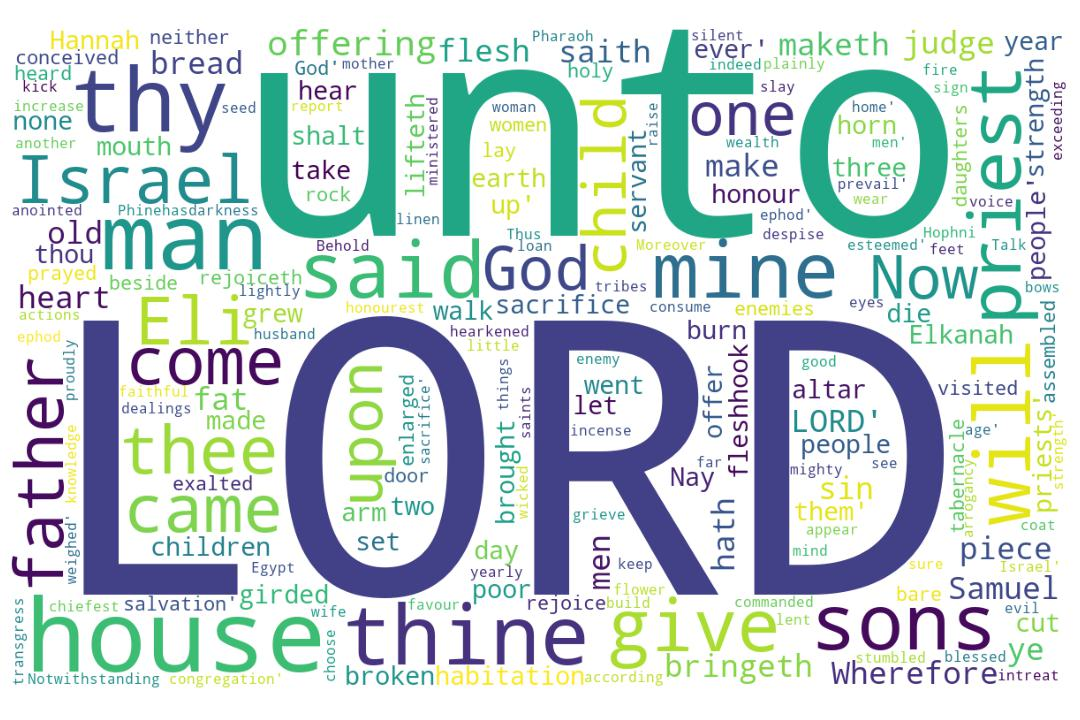
\includegraphics[width=\linewidth]{09OT-1Samuel/1Samuel2-WordCloud.jpg}
  \caption{1 Samuel 2 Word Cloud}
  \label{fig:1 Samuel 2 Word Cloud}
\end{figure}




\marginpar{\scriptsize \centering \fcolorbox{bone}{lime}{\textbf{HANNAH's HAPPINESS}}\\ (1 Samuel 2:1-11) \begin{compactenum}[I.][8]
    \item Her \textbf{Prayer}  \index[scripture]{1Samuel!1Sa 02:01}(1Sa 2:1) 
    \item Her \textbf{Proof}  \index[scripture]{1Samuel!1Sa 02:01}(1Sa 2:1)
    \item Her \textbf{Praise}  \index[scripture]{1Samuel!1Sa 02:02--02}(1Sa 2:2--3)
    \item Her \textbf{Perspective}  %\index[scripture]{1Samuel!1Sa 02:02--02}(1Sa 2:2--3)
    \item Her \textbf{Comparisons} \index[scripture]{1Samuel!1Sa 02:04--08}  (1Sa 2:4--8)
    \item Her \textbf{Prophecy}  \index[scripture]{1Samuel!1Sa 02:10}(1Sa 2:10)
    \item Her \textbf{Performance}  \index[scripture]{1Samuel!1Sa 02:11}(1Sa 2:11) -- fulfills her promise
\end{compactenum}}






\footnote{\textcolor[cmyk]{0.99998,1,0,0}{\hyperlink{TOC}{Return to end of Table of Contents.}}}\footnote{\href{https://audiobible.com/bible/1_samuel_2.html}{\textcolor[cmyk]{0.99998,1,0,0}{1 Samuel 2 Audio}}}\textcolor[cmyk]{0.99998,1,0,0}{And Hannah \fcolorbox{bone}{lime}{prayed}, and said, My heart rejoiceth in the LORD, mine horn is exalted in the LORD: my mouth is \fcolorbox{bone}{lime}{enlarged} over mine enemies; because I rejoice in thy salvation.}
[2] \textcolor[cmyk]{0.99998,1,0,0}{\emph{There} \emph{is} none holy as the LORD: for \emph{there} \emph{is} none beside thee: neither \emph{is} \emph{there} any rock like our God.}
[3] \textcolor[cmyk]{0.99998,1,0,0}{Talk no more so exceeding proudly; let \emph{not} arrogancy come out of your mouth: for the LORD \emph{is} \fcolorbox{bone}{bone}{a} God of knowledge, and by him actions are \fcolorbox{bone}{lime}{weighed}.}
[4] \textcolor[cmyk]{0.99998,1,0,0}{The bows of the mighty men \emph{are} broken, and they that stumbled are girded with strength.}
[5] \textcolor[cmyk]{0.99998,1,0,0}{\emph{They} \emph{that} \emph{were} full have hired out themselves for bread; and \emph{they} \emph{that} \emph{were} hungry ceased: so that the barren hath born seven; and she that hath many children is waxed feeble.}
[6] \textcolor[cmyk]{0.99998,1,0,0}{The LORD killeth, and maketh alive: he bringeth down to the grave, and bringeth up.}
[7] \textcolor[cmyk]{0.99998,1,0,0}{The LORD maketh poor, and maketh rich: he bringeth low, and lifteth up.}
[8] \textcolor[cmyk]{0.99998,1,0,0}{He raiseth up \fcolorbox{bone}{lime}{the poor} out of the dust, \emph{and} lifteth up the beggar from the dunghill, to set \emph{them} among princes, and to make them inherit the throne of glory: for the pillars of the earth \emph{are} the LORD'S, and he hath set the world upon them.}
[9] \textcolor[cmyk]{0.99998,1,0,0}{He will keep the feet of his saints, and the wicked shall be silent in darkness; for by strength shall no man prevail.}
[10] \textcolor[cmyk]{0.99998,1,0,0}{The adversaries of the LORD shall be broken to pieces; out of heaven shall he thunder upon them: the LORD shall judge the ends of the earth; and he shall give strength \fcolorbox{bone}{bone}{unto} his king, and \fcolorbox{bone}{lime}{exalt the horn} of his anointed.}
[11] \textcolor[cmyk]{0.99998,1,0,0}{And Elkanah went to Ramah to his house. And \fcolorbox{bone}{lime}{the child did minister} \fcolorbox{bone}{bone}{unto} the LORD before Eli the priest.}\\
\\
\P \textcolor[cmyk]{0.99998,1,0,0}{Now the sons of Eli \emph{were} sons of Belial; they knew not the LORD.}
[13] \textcolor[cmyk]{0.99998,1,0,0}{And the priests' custom with the people \emph{was,} \emph{that}, when any man offered sacrifice, the priest's servant came, while the flesh was in seething, with \fcolorbox{bone}{bone}{a} fleshhook of three teeth in his hand;}
[14] \textcolor[cmyk]{0.99998,1,0,0}{And he struck \emph{it} into the pan, or kettle, or caldron, or pot; all that the fleshhook brought up the priest took for himself. So they did in Shiloh \fcolorbox{bone}{bone}{unto} all the Israelites that came thither.}
[15] \textcolor[cmyk]{0.99998,1,0,0}{Also before they burnt the fat, the priest's servant came, and said to the man that sacrificed, Give flesh to roast for the priest; for he will not have sodden flesh of thee, but raw.}
[16] \textcolor[cmyk]{0.99998,1,0,0}{And \emph{if} any man said \fcolorbox{bone}{bone}{unto} him, Let them not fail to burn the fat presently, and \emph{then} take \emph{as} \emph{much} as thy soul desireth; then he would answer him, \emph{Nay}; but thou shalt give \emph{it} \emph{me} now: and if not, I will take \emph{it} by force.}
[17] \textcolor[cmyk]{0.99998,1,0,0}{Wherefore the sin of the young men was very great before the LORD: for men abhorred the offering of the LORD.}\\
\\
\P \textcolor[cmyk]{0.99998,1,0,0}{But Samuel ministered before the LORD, \emph{being} \fcolorbox{bone}{bone}{a} child, girded with \fcolorbox{bone}{bone}{a} linen ephod.}
[19] \textcolor[cmyk]{0.99998,1,0,0}{Moreover his mother made him \fcolorbox{bone}{bone}{a} little coat, and brought \emph{it} to him from year to year, when she came up with her husband to offer the yearly sacrifice.}\\
\\
\P \textcolor[cmyk]{0.99998,1,0,0}{And Eli blessed Elkanah and his wife, and said, The LORD give thee seed of this woman for the loan which is lent to the LORD. And they went \fcolorbox{bone}{bone}{unto} their own home.}
[21] \textcolor[cmyk]{0.99998,1,0,0}{And the LORD visited Hannah, so that she conceived, and bare three sons and two daughters. And the child Samuel grew before the LORD.}\\
\\
\P \textcolor[cmyk]{0.99998,1,0,0}{Now Eli was very old, and heard all that his sons did \fcolorbox{bone}{bone}{unto} all Israel; and how they lay with the women that assembled \emph{at} the door of the tabernacle of the congregation.}
[23] \textcolor[cmyk]{0.99998,1,0,0}{And he said \fcolorbox{bone}{bone}{unto} them, Why do ye such things? for I hear of your evil dealings by all this people.}
[24] \textcolor[cmyk]{0.99998,1,0,0}{Nay, my sons; for \emph{it} \emph{is} no good report that I hear: ye make the LORD'S people to transgress.}
[25] \textcolor[cmyk]{0.99998,1,0,0}{If one man sin against another, the judge shall judge him: but if \fcolorbox{bone}{bone}{a} man sin against the LORD, who shall intreat for him? Notwithstanding they hearkened not \fcolorbox{bone}{bone}{unto} the voice of their father, because the LORD would slay them.}
[26] \textcolor[cmyk]{0.99998,1,0,0}{And the child Samuel grew on, and was in favour both with the LORD, and also with men.}\\
\\
\P \textcolor[cmyk]{0.99998,1,0,0}{And there came \fcolorbox{bone}{bone}{a} man of God \fcolorbox{bone}{bone}{unto} Eli, and said \fcolorbox{bone}{bone}{unto} him, Thus saith the LORD, Did I plainly appear \fcolorbox{bone}{bone}{unto} the house of thy father, when they were in Egypt in Pharaoh's house?}
[28] \textcolor[cmyk]{0.99998,1,0,0}{And did I choose him out of all the tribes of Israel \emph{to} \emph{be} my priest, to offer upon mine altar, to burn incense, to wear an ephod before me? and did I give \fcolorbox{bone}{bone}{unto} the house of thy father all the offerings made by fire of the children of Israel?}
[29] \textcolor[cmyk]{0.99998,1,0,0}{Wherefore kick ye at my sacrifice and at mine offering, which I have commanded \emph{in} \emph{my} habitation; and honourest thy sons above me, to make yourselves fat with the chiefest of all the offerings of Israel my people?}
[30] \textcolor[cmyk]{0.99998,1,0,0}{Wherefore the LORD God of Israel saith, I said indeed \emph{that} thy house, and the house of thy father, should walk before me for ever: but now the LORD saith, Be it far from me; for them that honour me I will honour, and they that despise me shall be lightly esteemed.}
[31] \textcolor[cmyk]{0.99998,1,0,0}{Behold, the days come, that I will cut off thine arm, and the arm of thy father's house, that there shall not be an old man in thine house.}
[32] \textcolor[cmyk]{0.99998,1,0,0}{And thou shalt see an enemy \emph{in} \emph{my} habitation, in all \emph{the} \emph{wealth} which \emph{God} shall give Israel: and there shall not be an old man in thine house for ever.}
[33] \textcolor[cmyk]{0.99998,1,0,0}{And the man of thine, \emph{whom} I shall not cut off from mine altar, \emph{shall} \emph{be} to consume thine eyes, and to grieve thine heart: and all the increase of thine house shall die in the flower of their age.}
[34] \textcolor[cmyk]{0.99998,1,0,0}{And this \emph{shall} \emph{be} \fcolorbox{bone}{bone}{a} sign \fcolorbox{bone}{bone}{unto} thee, that shall come upon thy two sons, on Hophni and Phinehas; in one day they shall die both of them.}
[35] \textcolor[cmyk]{0.99998,1,0,0}{And I will raise me up \fcolorbox{bone}{bone}{a} faithful priest, \emph{that} shall do according to \emph{that} which \emph{is} in mine heart and in my mind: and I will build him \fcolorbox{bone}{bone}{a} sure house; and he shall walk before mine anointed for ever.}
[36] \textcolor[cmyk]{0.99998,1,0,0}{And it shall come to pass, \emph{that} every one that is left in thine house shall come \emph{and} crouch to him for \fcolorbox{bone}{bone}{a} piece of silver and \fcolorbox{bone}{bone}{a} morsel of bread, and shall say, Put me, I pray thee, into one of the priests' offices, that I may eat \fcolorbox{bone}{bone}{a} piece of bread.}
\section{1 Samuel 2 Comments}

\subsection{Numeric Nuggets}
\textbf{13: } Verse 7 has 13 words. Verses 6 and 18 have 13 unique words. The words ``a'' and ``unto'' are used 13 times in the chapter.
%\index[NWIV]{27!1Samuel!1Sa 12:1}\index[AWIP]{And!1Samuel!1Sa 12:1}\index[AWIP]{Samuel!1Samuel!1Sa 12:1}\index[AWIP]{said!1Samuel!1Sa 12:1}\index[AWIP]{said!1Samuel!1Sa 12:1 (2)}\index[AWIP]{unto!1Samuel!1Sa 12:1}\index[AWIP]{unto!1Samuel!1Sa 12:1 (2)}\index[AWIP]{unto!1Samuel!1Sa 12:1 (3)}\index[AWIP]{all!1Samuel!1Sa 12:1}\index[AWIP]{all!1Samuel!1Sa 12:1 (2)}\index[AWIP]{Israel!1Samuel!1Sa 12:1}\index[AWIP]{Behold!1Samuel!1Sa 12:1}\index[AWIP]{I!1Samuel!1Sa 12:1}\index[AWIP]{have!1Samuel!1Sa 12:1}\index[AWIP]{have!1Samuel!1Sa 12:1 (2)}\index[AWIP]{hearkened!1Samuel!1Sa 12:1}\index[AWIP]{your!1Samuel!1Sa 12:1}\index[AWIP]{voice!1Samuel!1Sa 12:1}\index[AWIP]{in!1Samuel!1Sa 12:1}\index[AWIP]{that!1Samuel!1Sa 12:1}\index[AWIP]{ye!1Samuel!1Sa 12:1}\index[AWIP]{me!1Samuel!1Sa 12:1}\index[AWIP]{and!1Samuel!1Sa 12:1}\index[AWIP]{made!1Samuel!1Sa 12:1}\index[AWIP]{a!1Samuel!1Sa 12:1}\index[AWIP]{king!1Samuel!1Sa 12:1}\index[AWIP]{over!1Samuel!1Sa 12:1}\index[AWIP]{you!1Samuel!1Sa 12:1}

\index[NWIV]{33!1Samuel!1Sa 12:2}\index[AWIP]{And!1Samuel!1Sa 12:2}\index[AWIP]{now!1Samuel!1Sa 12:2}\index[AWIP]{behold!1Samuel!1Sa 12:2}\index[AWIP]{behold!1Samuel!1Sa 12:2 (2)}\index[AWIP]{the!1Samuel!1Sa 12:2}\index[AWIP]{king!1Samuel!1Sa 12:2}\index[AWIP]{walketh!1Samuel!1Sa 12:2}\index[AWIP]{before!1Samuel!1Sa 12:2}\index[AWIP]{before!1Samuel!1Sa 12:2 (2)}\index[AWIP]{you!1Samuel!1Sa 12:2}\index[AWIP]{you!1Samuel!1Sa 12:2 (2)}\index[AWIP]{you!1Samuel!1Sa 12:2 (3)}\index[AWIP]{and!1Samuel!1Sa 12:2}\index[AWIP]{and!1Samuel!1Sa 12:2 (2)}\index[AWIP]{and!1Samuel!1Sa 12:2 (3)}\index[AWIP]{and!1Samuel!1Sa 12:2 (4)}\index[AWIP]{I!1Samuel!1Sa 12:2}\index[AWIP]{I!1Samuel!1Sa 12:2 (2)}\index[AWIP]{am!1Samuel!1Sa 12:2}\index[AWIP]{old!1Samuel!1Sa 12:2}\index[AWIP]{grayheaded!1Samuel!1Sa 12:2}\index[AWIP]{my!1Samuel!1Sa 12:2}\index[AWIP]{my!1Samuel!1Sa 12:2 (2)}\index[AWIP]{sons!1Samuel!1Sa 12:2}\index[AWIP]{\emph{are}!1Samuel!1Sa 12:2}\index[AWIP]{with!1Samuel!1Sa 12:2}\index[AWIP]{have!1Samuel!1Sa 12:2}\index[AWIP]{walked!1Samuel!1Sa 12:2}\index[AWIP]{from!1Samuel!1Sa 12:2}\index[AWIP]{childhood!1Samuel!1Sa 12:2}\index[AWIP]{unto!1Samuel!1Sa 12:2}\index[AWIP]{this!1Samuel!1Sa 12:2}\index[AWIP]{day!1Samuel!1Sa 12:2}\index[AWIP]{\emph{are}!1Samuel!1Sa 12:2}

\index[NWIV]{54!1Samuel!1Sa 12:3}\index[AWIP]{Behold!1Samuel!1Sa 12:3}\index[AWIP]{here!1Samuel!1Sa 12:3}\index[AWIP]{I!1Samuel!1Sa 12:3}\index[AWIP]{I!1Samuel!1Sa 12:3 (2)}\index[AWIP]{I!1Samuel!1Sa 12:3 (3)}\index[AWIP]{I!1Samuel!1Sa 12:3 (4)}\index[AWIP]{I!1Samuel!1Sa 12:3 (5)}\index[AWIP]{I!1Samuel!1Sa 12:3 (6)}\index[AWIP]{I!1Samuel!1Sa 12:3 (7)}\index[AWIP]{\emph{am}!1Samuel!1Sa 12:3}\index[AWIP]{witness!1Samuel!1Sa 12:3}\index[AWIP]{against!1Samuel!1Sa 12:3}\index[AWIP]{me!1Samuel!1Sa 12:3}\index[AWIP]{before!1Samuel!1Sa 12:3}\index[AWIP]{before!1Samuel!1Sa 12:3 (2)}\index[AWIP]{the!1Samuel!1Sa 12:3}\index[AWIP]{LORD!1Samuel!1Sa 12:3}\index[AWIP]{and!1Samuel!1Sa 12:3}\index[AWIP]{and!1Samuel!1Sa 12:3 (2)}\index[AWIP]{his!1Samuel!1Sa 12:3}\index[AWIP]{anointed!1Samuel!1Sa 12:3}\index[AWIP]{whose!1Samuel!1Sa 12:3}\index[AWIP]{whose!1Samuel!1Sa 12:3 (2)}\index[AWIP]{whose!1Samuel!1Sa 12:3 (3)}\index[AWIP]{ox!1Samuel!1Sa 12:3}\index[AWIP]{have!1Samuel!1Sa 12:3}\index[AWIP]{have!1Samuel!1Sa 12:3 (2)}\index[AWIP]{have!1Samuel!1Sa 12:3 (3)}\index[AWIP]{have!1Samuel!1Sa 12:3 (4)}\index[AWIP]{have!1Samuel!1Sa 12:3 (5)}\index[AWIP]{taken?!1Samuel!1Sa 12:3}\index[AWIP]{taken?!1Samuel!1Sa 12:3 (2)}\index[AWIP]{or!1Samuel!1Sa 12:3}\index[AWIP]{or!1Samuel!1Sa 12:3 (2)}\index[AWIP]{or!1Samuel!1Sa 12:3 (3)}\index[AWIP]{ass!1Samuel!1Sa 12:3}\index[AWIP]{whom!1Samuel!1Sa 12:3}\index[AWIP]{whom!1Samuel!1Sa 12:3 (2)}\index[AWIP]{defrauded?!1Samuel!1Sa 12:3}\index[AWIP]{oppressed?!1Samuel!1Sa 12:3}\index[AWIP]{of!1Samuel!1Sa 12:3}\index[AWIP]{hand!1Samuel!1Sa 12:3}\index[AWIP]{received!1Samuel!1Sa 12:3}\index[AWIP]{\emph{any}!1Samuel!1Sa 12:3}\index[AWIP]{bribe!1Samuel!1Sa 12:3}\index[AWIP]{to!1Samuel!1Sa 12:3}\index[AWIP]{blind!1Samuel!1Sa 12:3}\index[AWIP]{mine!1Samuel!1Sa 12:3}\index[AWIP]{eyes!1Samuel!1Sa 12:3}\index[AWIP]{therewith?!1Samuel!1Sa 12:3}\index[AWIP]{will!1Samuel!1Sa 12:3}\index[AWIP]{restore!1Samuel!1Sa 12:3}\index[AWIP]{it!1Samuel!1Sa 12:3}\index[AWIP]{you!1Samuel!1Sa 12:3}\index[AWIP]{\emph{am}!1Samuel!1Sa 12:3}\index[AWIP]{\emph{any}!1Samuel!1Sa 12:3}

\index[NWIV]{20!1Samuel!1Sa 12:4}\index[AWIP]{And!1Samuel!1Sa 12:4}\index[AWIP]{they!1Samuel!1Sa 12:4}\index[AWIP]{said!1Samuel!1Sa 12:4}\index[AWIP]{Thou!1Samuel!1Sa 12:4}\index[AWIP]{hast!1Samuel!1Sa 12:4}\index[AWIP]{hast!1Samuel!1Sa 12:4 (2)}\index[AWIP]{not!1Samuel!1Sa 12:4}\index[AWIP]{defrauded!1Samuel!1Sa 12:4}\index[AWIP]{us!1Samuel!1Sa 12:4}\index[AWIP]{us!1Samuel!1Sa 12:4 (2)}\index[AWIP]{nor!1Samuel!1Sa 12:4}\index[AWIP]{oppressed!1Samuel!1Sa 12:4}\index[AWIP]{neither!1Samuel!1Sa 12:4}\index[AWIP]{thou!1Samuel!1Sa 12:4}\index[AWIP]{taken!1Samuel!1Sa 12:4}\index[AWIP]{ought!1Samuel!1Sa 12:4}\index[AWIP]{of!1Samuel!1Sa 12:4}\index[AWIP]{any!1Samuel!1Sa 12:4}\index[AWIP]{man's!1Samuel!1Sa 12:4}\index[AWIP]{hand!1Samuel!1Sa 12:4}

\index[NWIV]{33!1Samuel!1Sa 12:5}\index[AWIP]{And!1Samuel!1Sa 12:5}\index[AWIP]{And!1Samuel!1Sa 12:5 (2)}\index[AWIP]{he!1Samuel!1Sa 12:5}\index[AWIP]{said!1Samuel!1Sa 12:5}\index[AWIP]{unto!1Samuel!1Sa 12:5}\index[AWIP]{them!1Samuel!1Sa 12:5}\index[AWIP]{The!1Samuel!1Sa 12:5}\index[AWIP]{LORD!1Samuel!1Sa 12:5}\index[AWIP]{\emph{is}!1Samuel!1Sa 12:5}\index[AWIP]{\emph{is}!1Samuel!1Sa 12:5 (2)}\index[AWIP]{\emph{is}!1Samuel!1Sa 12:5 (3)}\index[AWIP]{witness!1Samuel!1Sa 12:5}\index[AWIP]{witness!1Samuel!1Sa 12:5 (2)}\index[AWIP]{witness!1Samuel!1Sa 12:5 (3)}\index[AWIP]{against!1Samuel!1Sa 12:5}\index[AWIP]{you!1Samuel!1Sa 12:5}\index[AWIP]{and!1Samuel!1Sa 12:5}\index[AWIP]{his!1Samuel!1Sa 12:5}\index[AWIP]{anointed!1Samuel!1Sa 12:5}\index[AWIP]{this!1Samuel!1Sa 12:5}\index[AWIP]{day!1Samuel!1Sa 12:5}\index[AWIP]{that!1Samuel!1Sa 12:5}\index[AWIP]{ye!1Samuel!1Sa 12:5}\index[AWIP]{have!1Samuel!1Sa 12:5}\index[AWIP]{not!1Samuel!1Sa 12:5}\index[AWIP]{found!1Samuel!1Sa 12:5}\index[AWIP]{ought!1Samuel!1Sa 12:5}\index[AWIP]{in!1Samuel!1Sa 12:5}\index[AWIP]{my!1Samuel!1Sa 12:5}\index[AWIP]{hand!1Samuel!1Sa 12:5}\index[AWIP]{they!1Samuel!1Sa 12:5}\index[AWIP]{answered!1Samuel!1Sa 12:5}\index[AWIP]{\emph{He}!1Samuel!1Sa 12:5}\index[AWIP]{\emph{is}!1Samuel!1Sa 12:5}\index[AWIP]{\emph{is}!1Samuel!1Sa 12:5 (2)}\index[AWIP]{\emph{is}!1Samuel!1Sa 12:5 (3)}\index[AWIP]{\emph{He}!1Samuel!1Sa 12:5}

\index[NWIV]{27!1Samuel!1Sa 12:6}\index[AWIP]{And!1Samuel!1Sa 12:6}\index[AWIP]{Samuel!1Samuel!1Sa 12:6}\index[AWIP]{said!1Samuel!1Sa 12:6}\index[AWIP]{unto!1Samuel!1Sa 12:6}\index[AWIP]{the!1Samuel!1Sa 12:6}\index[AWIP]{the!1Samuel!1Sa 12:6 (2)}\index[AWIP]{the!1Samuel!1Sa 12:6 (3)}\index[AWIP]{people!1Samuel!1Sa 12:6}\index[AWIP]{\emph{It}!1Samuel!1Sa 12:6}\index[AWIP]{\emph{is}!1Samuel!1Sa 12:6}\index[AWIP]{LORD!1Samuel!1Sa 12:6}\index[AWIP]{that!1Samuel!1Sa 12:6}\index[AWIP]{that!1Samuel!1Sa 12:6 (2)}\index[AWIP]{advanced!1Samuel!1Sa 12:6}\index[AWIP]{Moses!1Samuel!1Sa 12:6}\index[AWIP]{and!1Samuel!1Sa 12:6}\index[AWIP]{and!1Samuel!1Sa 12:6 (2)}\index[AWIP]{Aaron!1Samuel!1Sa 12:6}\index[AWIP]{brought!1Samuel!1Sa 12:6}\index[AWIP]{your!1Samuel!1Sa 12:6}\index[AWIP]{fathers!1Samuel!1Sa 12:6}\index[AWIP]{up!1Samuel!1Sa 12:6}\index[AWIP]{out!1Samuel!1Sa 12:6}\index[AWIP]{of!1Samuel!1Sa 12:6}\index[AWIP]{of!1Samuel!1Sa 12:6 (2)}\index[AWIP]{land!1Samuel!1Sa 12:6}\index[AWIP]{Egypt!1Samuel!1Sa 12:6}\index[AWIP]{\emph{It}!1Samuel!1Sa 12:6}\index[AWIP]{\emph{is}!1Samuel!1Sa 12:6}

\index[NWIV]{30!1Samuel!1Sa 12:7}\index[AWIP]{Now!1Samuel!1Sa 12:7}\index[AWIP]{therefore!1Samuel!1Sa 12:7}\index[AWIP]{stand!1Samuel!1Sa 12:7}\index[AWIP]{still!1Samuel!1Sa 12:7}\index[AWIP]{that!1Samuel!1Sa 12:7}\index[AWIP]{I!1Samuel!1Sa 12:7}\index[AWIP]{may!1Samuel!1Sa 12:7}\index[AWIP]{reason!1Samuel!1Sa 12:7}\index[AWIP]{with!1Samuel!1Sa 12:7}\index[AWIP]{you!1Samuel!1Sa 12:7}\index[AWIP]{you!1Samuel!1Sa 12:7 (2)}\index[AWIP]{before!1Samuel!1Sa 12:7}\index[AWIP]{the!1Samuel!1Sa 12:7}\index[AWIP]{the!1Samuel!1Sa 12:7 (2)}\index[AWIP]{the!1Samuel!1Sa 12:7 (3)}\index[AWIP]{LORD!1Samuel!1Sa 12:7}\index[AWIP]{LORD!1Samuel!1Sa 12:7 (2)}\index[AWIP]{of!1Samuel!1Sa 12:7}\index[AWIP]{of!1Samuel!1Sa 12:7 (2)}\index[AWIP]{all!1Samuel!1Sa 12:7}\index[AWIP]{righteous!1Samuel!1Sa 12:7}\index[AWIP]{acts!1Samuel!1Sa 12:7}\index[AWIP]{which!1Samuel!1Sa 12:7}\index[AWIP]{he!1Samuel!1Sa 12:7}\index[AWIP]{did!1Samuel!1Sa 12:7}\index[AWIP]{to!1Samuel!1Sa 12:7}\index[AWIP]{to!1Samuel!1Sa 12:7 (2)}\index[AWIP]{and!1Samuel!1Sa 12:7}\index[AWIP]{your!1Samuel!1Sa 12:7}\index[AWIP]{fathers!1Samuel!1Sa 12:7}

\index[NWIV]{35!1Samuel!1Sa 12:8}\index[AWIP]{When!1Samuel!1Sa 12:8}\index[AWIP]{Jacob!1Samuel!1Sa 12:8}\index[AWIP]{was!1Samuel!1Sa 12:8}\index[AWIP]{come!1Samuel!1Sa 12:8}\index[AWIP]{into!1Samuel!1Sa 12:8}\index[AWIP]{Egypt!1Samuel!1Sa 12:8}\index[AWIP]{Egypt!1Samuel!1Sa 12:8 (2)}\index[AWIP]{and!1Samuel!1Sa 12:8}\index[AWIP]{and!1Samuel!1Sa 12:8 (2)}\index[AWIP]{and!1Samuel!1Sa 12:8 (3)}\index[AWIP]{your!1Samuel!1Sa 12:8}\index[AWIP]{your!1Samuel!1Sa 12:8 (2)}\index[AWIP]{fathers!1Samuel!1Sa 12:8}\index[AWIP]{fathers!1Samuel!1Sa 12:8 (2)}\index[AWIP]{cried!1Samuel!1Sa 12:8}\index[AWIP]{unto!1Samuel!1Sa 12:8}\index[AWIP]{the!1Samuel!1Sa 12:8}\index[AWIP]{the!1Samuel!1Sa 12:8 (2)}\index[AWIP]{LORD!1Samuel!1Sa 12:8}\index[AWIP]{LORD!1Samuel!1Sa 12:8 (2)}\index[AWIP]{then!1Samuel!1Sa 12:8}\index[AWIP]{sent!1Samuel!1Sa 12:8}\index[AWIP]{Moses!1Samuel!1Sa 12:8}\index[AWIP]{Aaron!1Samuel!1Sa 12:8}\index[AWIP]{which!1Samuel!1Sa 12:8}\index[AWIP]{brought!1Samuel!1Sa 12:8}\index[AWIP]{forth!1Samuel!1Sa 12:8}\index[AWIP]{out!1Samuel!1Sa 12:8}\index[AWIP]{of!1Samuel!1Sa 12:8}\index[AWIP]{made!1Samuel!1Sa 12:8}\index[AWIP]{them!1Samuel!1Sa 12:8}\index[AWIP]{dwell!1Samuel!1Sa 12:8}\index[AWIP]{in!1Samuel!1Sa 12:8}\index[AWIP]{this!1Samuel!1Sa 12:8}\index[AWIP]{place!1Samuel!1Sa 12:8}

\index[NWIV]{43!1Samuel!1Sa 12:9}\index[AWIP]{And!1Samuel!1Sa 12:9}\index[AWIP]{when!1Samuel!1Sa 12:9}\index[AWIP]{they!1Samuel!1Sa 12:9}\index[AWIP]{they!1Samuel!1Sa 12:9 (2)}\index[AWIP]{forgat!1Samuel!1Sa 12:9}\index[AWIP]{the!1Samuel!1Sa 12:9}\index[AWIP]{the!1Samuel!1Sa 12:9 (2)}\index[AWIP]{the!1Samuel!1Sa 12:9 (3)}\index[AWIP]{the!1Samuel!1Sa 12:9 (4)}\index[AWIP]{the!1Samuel!1Sa 12:9 (5)}\index[AWIP]{the!1Samuel!1Sa 12:9 (6)}\index[AWIP]{the!1Samuel!1Sa 12:9 (7)}\index[AWIP]{LORD!1Samuel!1Sa 12:9}\index[AWIP]{their!1Samuel!1Sa 12:9}\index[AWIP]{God!1Samuel!1Sa 12:9}\index[AWIP]{he!1Samuel!1Sa 12:9}\index[AWIP]{sold!1Samuel!1Sa 12:9}\index[AWIP]{them!1Samuel!1Sa 12:9}\index[AWIP]{them!1Samuel!1Sa 12:9 (2)}\index[AWIP]{into!1Samuel!1Sa 12:9}\index[AWIP]{into!1Samuel!1Sa 12:9 (2)}\index[AWIP]{into!1Samuel!1Sa 12:9 (3)}\index[AWIP]{hand!1Samuel!1Sa 12:9}\index[AWIP]{hand!1Samuel!1Sa 12:9 (2)}\index[AWIP]{hand!1Samuel!1Sa 12:9 (3)}\index[AWIP]{of!1Samuel!1Sa 12:9}\index[AWIP]{of!1Samuel!1Sa 12:9 (2)}\index[AWIP]{of!1Samuel!1Sa 12:9 (3)}\index[AWIP]{of!1Samuel!1Sa 12:9 (4)}\index[AWIP]{of!1Samuel!1Sa 12:9 (5)}\index[AWIP]{of!1Samuel!1Sa 12:9 (6)}\index[AWIP]{Sisera!1Samuel!1Sa 12:9}\index[AWIP]{captain!1Samuel!1Sa 12:9}\index[AWIP]{host!1Samuel!1Sa 12:9}\index[AWIP]{Hazor!1Samuel!1Sa 12:9}\index[AWIP]{and!1Samuel!1Sa 12:9}\index[AWIP]{and!1Samuel!1Sa 12:9 (2)}\index[AWIP]{and!1Samuel!1Sa 12:9 (3)}\index[AWIP]{Philistines!1Samuel!1Sa 12:9}\index[AWIP]{king!1Samuel!1Sa 12:9}\index[AWIP]{Moab!1Samuel!1Sa 12:9}\index[AWIP]{fought!1Samuel!1Sa 12:9}\index[AWIP]{against!1Samuel!1Sa 12:9}

\index[NWIV]{39!1Samuel!1Sa 12:10}\index[AWIP]{And!1Samuel!1Sa 12:10}\index[AWIP]{they!1Samuel!1Sa 12:10}\index[AWIP]{cried!1Samuel!1Sa 12:10}\index[AWIP]{unto!1Samuel!1Sa 12:10}\index[AWIP]{the!1Samuel!1Sa 12:10}\index[AWIP]{the!1Samuel!1Sa 12:10 (2)}\index[AWIP]{the!1Samuel!1Sa 12:10 (3)}\index[AWIP]{LORD!1Samuel!1Sa 12:10}\index[AWIP]{LORD!1Samuel!1Sa 12:10 (2)}\index[AWIP]{and!1Samuel!1Sa 12:10}\index[AWIP]{and!1Samuel!1Sa 12:10 (2)}\index[AWIP]{and!1Samuel!1Sa 12:10 (3)}\index[AWIP]{and!1Samuel!1Sa 12:10 (4)}\index[AWIP]{said!1Samuel!1Sa 12:10}\index[AWIP]{We!1Samuel!1Sa 12:10}\index[AWIP]{have!1Samuel!1Sa 12:10}\index[AWIP]{have!1Samuel!1Sa 12:10 (2)}\index[AWIP]{have!1Samuel!1Sa 12:10 (3)}\index[AWIP]{sinned!1Samuel!1Sa 12:10}\index[AWIP]{because!1Samuel!1Sa 12:10}\index[AWIP]{we!1Samuel!1Sa 12:10}\index[AWIP]{we!1Samuel!1Sa 12:10 (2)}\index[AWIP]{forsaken!1Samuel!1Sa 12:10}\index[AWIP]{served!1Samuel!1Sa 12:10}\index[AWIP]{Baalim!1Samuel!1Sa 12:10}\index[AWIP]{Ashtaroth!1Samuel!1Sa 12:10}\index[AWIP]{but!1Samuel!1Sa 12:10}\index[AWIP]{now!1Samuel!1Sa 12:10}\index[AWIP]{deliver!1Samuel!1Sa 12:10}\index[AWIP]{us!1Samuel!1Sa 12:10}\index[AWIP]{out!1Samuel!1Sa 12:10}\index[AWIP]{of!1Samuel!1Sa 12:10}\index[AWIP]{of!1Samuel!1Sa 12:10 (2)}\index[AWIP]{hand!1Samuel!1Sa 12:10}\index[AWIP]{our!1Samuel!1Sa 12:10}\index[AWIP]{enemies!1Samuel!1Sa 12:10}\index[AWIP]{will!1Samuel!1Sa 12:10}\index[AWIP]{serve!1Samuel!1Sa 12:10}\index[AWIP]{thee!1Samuel!1Sa 12:10}

\index[NWIV]{28!1Samuel!1Sa 12:11}\index[AWIP]{And!1Samuel!1Sa 12:11}\index[AWIP]{the!1Samuel!1Sa 12:11}\index[AWIP]{the!1Samuel!1Sa 12:11 (2)}\index[AWIP]{LORD!1Samuel!1Sa 12:11}\index[AWIP]{sent!1Samuel!1Sa 12:11}\index[AWIP]{Jerubbaal!1Samuel!1Sa 12:11}\index[AWIP]{and!1Samuel!1Sa 12:11}\index[AWIP]{and!1Samuel!1Sa 12:11 (2)}\index[AWIP]{and!1Samuel!1Sa 12:11 (3)}\index[AWIP]{and!1Samuel!1Sa 12:11 (4)}\index[AWIP]{and!1Samuel!1Sa 12:11 (5)}\index[AWIP]{Bedan!1Samuel!1Sa 12:11}\index[AWIP]{Jephthah!1Samuel!1Sa 12:11}\index[AWIP]{Samuel!1Samuel!1Sa 12:11}\index[AWIP]{delivered!1Samuel!1Sa 12:11}\index[AWIP]{you!1Samuel!1Sa 12:11}\index[AWIP]{out!1Samuel!1Sa 12:11}\index[AWIP]{of!1Samuel!1Sa 12:11}\index[AWIP]{of!1Samuel!1Sa 12:11 (2)}\index[AWIP]{hand!1Samuel!1Sa 12:11}\index[AWIP]{your!1Samuel!1Sa 12:11}\index[AWIP]{enemies!1Samuel!1Sa 12:11}\index[AWIP]{on!1Samuel!1Sa 12:11}\index[AWIP]{every!1Samuel!1Sa 12:11}\index[AWIP]{side!1Samuel!1Sa 12:11}\index[AWIP]{ye!1Samuel!1Sa 12:11}\index[AWIP]{dwelled!1Samuel!1Sa 12:11}\index[AWIP]{safe!1Samuel!1Sa 12:11}

\index[NWIV]{36!1Samuel!1Sa 12:12}\index[AWIP]{And!1Samuel!1Sa 12:12}\index[AWIP]{when!1Samuel!1Sa 12:12}\index[AWIP]{when!1Samuel!1Sa 12:12 (2)}\index[AWIP]{ye!1Samuel!1Sa 12:12}\index[AWIP]{ye!1Samuel!1Sa 12:12 (2)}\index[AWIP]{saw!1Samuel!1Sa 12:12}\index[AWIP]{that!1Samuel!1Sa 12:12}\index[AWIP]{Nahash!1Samuel!1Sa 12:12}\index[AWIP]{the!1Samuel!1Sa 12:12}\index[AWIP]{the!1Samuel!1Sa 12:12 (2)}\index[AWIP]{the!1Samuel!1Sa 12:12 (3)}\index[AWIP]{king!1Samuel!1Sa 12:12}\index[AWIP]{king!1Samuel!1Sa 12:12 (2)}\index[AWIP]{king!1Samuel!1Sa 12:12 (3)}\index[AWIP]{of!1Samuel!1Sa 12:12}\index[AWIP]{of!1Samuel!1Sa 12:12 (2)}\index[AWIP]{children!1Samuel!1Sa 12:12}\index[AWIP]{Ammon!1Samuel!1Sa 12:12}\index[AWIP]{came!1Samuel!1Sa 12:12}\index[AWIP]{against!1Samuel!1Sa 12:12}\index[AWIP]{you!1Samuel!1Sa 12:12}\index[AWIP]{said!1Samuel!1Sa 12:12}\index[AWIP]{unto!1Samuel!1Sa 12:12}\index[AWIP]{me!1Samuel!1Sa 12:12}\index[AWIP]{Nay!1Samuel!1Sa 12:12}\index[AWIP]{but!1Samuel!1Sa 12:12}\index[AWIP]{a!1Samuel!1Sa 12:12}\index[AWIP]{shall!1Samuel!1Sa 12:12}\index[AWIP]{reign!1Samuel!1Sa 12:12}\index[AWIP]{over!1Samuel!1Sa 12:12}\index[AWIP]{us!1Samuel!1Sa 12:12}\index[AWIP]{LORD!1Samuel!1Sa 12:12}\index[AWIP]{your!1Samuel!1Sa 12:12}\index[AWIP]{your!1Samuel!1Sa 12:12 (2)}\index[AWIP]{God!1Samuel!1Sa 12:12}\index[AWIP]{\emph{was}!1Samuel!1Sa 12:12}\index[AWIP]{\emph{was}!1Samuel!1Sa 12:12}

\index[NWIV]{24!1Samuel!1Sa 12:13}\index[AWIP]{Now!1Samuel!1Sa 12:13}\index[AWIP]{therefore!1Samuel!1Sa 12:13}\index[AWIP]{behold!1Samuel!1Sa 12:13}\index[AWIP]{behold!1Samuel!1Sa 12:13 (2)}\index[AWIP]{the!1Samuel!1Sa 12:13}\index[AWIP]{the!1Samuel!1Sa 12:13 (2)}\index[AWIP]{king!1Samuel!1Sa 12:13}\index[AWIP]{king!1Samuel!1Sa 12:13 (2)}\index[AWIP]{whom!1Samuel!1Sa 12:13}\index[AWIP]{whom!1Samuel!1Sa 12:13 (2)}\index[AWIP]{ye!1Samuel!1Sa 12:13}\index[AWIP]{ye!1Samuel!1Sa 12:13 (2)}\index[AWIP]{have!1Samuel!1Sa 12:13}\index[AWIP]{have!1Samuel!1Sa 12:13 (2)}\index[AWIP]{chosen!1Samuel!1Sa 12:13}\index[AWIP]{\emph{and}!1Samuel!1Sa 12:13}\index[AWIP]{desired!!1Samuel!1Sa 12:13}\index[AWIP]{and!1Samuel!1Sa 12:13}\index[AWIP]{LORD!1Samuel!1Sa 12:13}\index[AWIP]{hath!1Samuel!1Sa 12:13}\index[AWIP]{set!1Samuel!1Sa 12:13}\index[AWIP]{a!1Samuel!1Sa 12:13}\index[AWIP]{over!1Samuel!1Sa 12:13}\index[AWIP]{you!1Samuel!1Sa 12:13}\index[AWIP]{\emph{and}!1Samuel!1Sa 12:13}

\index[NWIV]{40!1Samuel!1Sa 12:14}\index[AWIP]{If!1Samuel!1Sa 12:14}\index[AWIP]{ye!1Samuel!1Sa 12:14}\index[AWIP]{ye!1Samuel!1Sa 12:14 (2)}\index[AWIP]{will!1Samuel!1Sa 12:14}\index[AWIP]{fear!1Samuel!1Sa 12:14}\index[AWIP]{the!1Samuel!1Sa 12:14}\index[AWIP]{the!1Samuel!1Sa 12:14 (2)}\index[AWIP]{the!1Samuel!1Sa 12:14 (3)}\index[AWIP]{the!1Samuel!1Sa 12:14 (4)}\index[AWIP]{the!1Samuel!1Sa 12:14 (5)}\index[AWIP]{LORD!1Samuel!1Sa 12:14}\index[AWIP]{LORD!1Samuel!1Sa 12:14 (2)}\index[AWIP]{LORD!1Samuel!1Sa 12:14 (3)}\index[AWIP]{and!1Samuel!1Sa 12:14}\index[AWIP]{and!1Samuel!1Sa 12:14 (2)}\index[AWIP]{and!1Samuel!1Sa 12:14 (3)}\index[AWIP]{and!1Samuel!1Sa 12:14 (4)}\index[AWIP]{serve!1Samuel!1Sa 12:14}\index[AWIP]{him!1Samuel!1Sa 12:14}\index[AWIP]{obey!1Samuel!1Sa 12:14}\index[AWIP]{his!1Samuel!1Sa 12:14}\index[AWIP]{voice!1Samuel!1Sa 12:14}\index[AWIP]{not!1Samuel!1Sa 12:14}\index[AWIP]{rebel!1Samuel!1Sa 12:14}\index[AWIP]{against!1Samuel!1Sa 12:14}\index[AWIP]{commandment!1Samuel!1Sa 12:14}\index[AWIP]{of!1Samuel!1Sa 12:14}\index[AWIP]{then!1Samuel!1Sa 12:14}\index[AWIP]{shall!1Samuel!1Sa 12:14}\index[AWIP]{both!1Samuel!1Sa 12:14}\index[AWIP]{also!1Samuel!1Sa 12:14}\index[AWIP]{king!1Samuel!1Sa 12:14}\index[AWIP]{that!1Samuel!1Sa 12:14}\index[AWIP]{reigneth!1Samuel!1Sa 12:14}\index[AWIP]{over!1Samuel!1Sa 12:14}\index[AWIP]{you!1Samuel!1Sa 12:14}\index[AWIP]{continue!1Samuel!1Sa 12:14}\index[AWIP]{following!1Samuel!1Sa 12:14}\index[AWIP]{your!1Samuel!1Sa 12:14}\index[AWIP]{God!1Samuel!1Sa 12:14}

\index[NWIV]{35!1Samuel!1Sa 12:15}\index[AWIP]{But!1Samuel!1Sa 12:15}\index[AWIP]{if!1Samuel!1Sa 12:15}\index[AWIP]{ye!1Samuel!1Sa 12:15}\index[AWIP]{will!1Samuel!1Sa 12:15}\index[AWIP]{not!1Samuel!1Sa 12:15}\index[AWIP]{obey!1Samuel!1Sa 12:15}\index[AWIP]{the!1Samuel!1Sa 12:15}\index[AWIP]{the!1Samuel!1Sa 12:15 (2)}\index[AWIP]{the!1Samuel!1Sa 12:15 (3)}\index[AWIP]{the!1Samuel!1Sa 12:15 (4)}\index[AWIP]{the!1Samuel!1Sa 12:15 (5)}\index[AWIP]{the!1Samuel!1Sa 12:15 (6)}\index[AWIP]{voice!1Samuel!1Sa 12:15}\index[AWIP]{of!1Samuel!1Sa 12:15}\index[AWIP]{of!1Samuel!1Sa 12:15 (2)}\index[AWIP]{of!1Samuel!1Sa 12:15 (3)}\index[AWIP]{LORD!1Samuel!1Sa 12:15}\index[AWIP]{LORD!1Samuel!1Sa 12:15 (2)}\index[AWIP]{LORD!1Samuel!1Sa 12:15 (3)}\index[AWIP]{but!1Samuel!1Sa 12:15}\index[AWIP]{rebel!1Samuel!1Sa 12:15}\index[AWIP]{against!1Samuel!1Sa 12:15}\index[AWIP]{against!1Samuel!1Sa 12:15 (2)}\index[AWIP]{against!1Samuel!1Sa 12:15 (3)}\index[AWIP]{commandment!1Samuel!1Sa 12:15}\index[AWIP]{then!1Samuel!1Sa 12:15}\index[AWIP]{shall!1Samuel!1Sa 12:15}\index[AWIP]{hand!1Samuel!1Sa 12:15}\index[AWIP]{be!1Samuel!1Sa 12:15}\index[AWIP]{you!1Samuel!1Sa 12:15}\index[AWIP]{as!1Samuel!1Sa 12:15}\index[AWIP]{\emph{it}!1Samuel!1Sa 12:15}\index[AWIP]{\emph{was}!1Samuel!1Sa 12:15}\index[AWIP]{your!1Samuel!1Sa 12:15}\index[AWIP]{fathers!1Samuel!1Sa 12:15}\index[AWIP]{\emph{it}!1Samuel!1Sa 12:15}\index[AWIP]{\emph{was}!1Samuel!1Sa 12:15}

\index[NWIV]{16!1Samuel!1Sa 12:16}\index[AWIP]{Now!1Samuel!1Sa 12:16}\index[AWIP]{therefore!1Samuel!1Sa 12:16}\index[AWIP]{stand!1Samuel!1Sa 12:16}\index[AWIP]{and!1Samuel!1Sa 12:16}\index[AWIP]{see!1Samuel!1Sa 12:16}\index[AWIP]{this!1Samuel!1Sa 12:16}\index[AWIP]{great!1Samuel!1Sa 12:16}\index[AWIP]{thing!1Samuel!1Sa 12:16}\index[AWIP]{which!1Samuel!1Sa 12:16}\index[AWIP]{the!1Samuel!1Sa 12:16}\index[AWIP]{LORD!1Samuel!1Sa 12:16}\index[AWIP]{will!1Samuel!1Sa 12:16}\index[AWIP]{do!1Samuel!1Sa 12:16}\index[AWIP]{before!1Samuel!1Sa 12:16}\index[AWIP]{your!1Samuel!1Sa 12:16}\index[AWIP]{eyes!1Samuel!1Sa 12:16}

\index[NWIV]{46!1Samuel!1Sa 12:17}\index[AWIP]{\emph{Is}!1Samuel!1Sa 12:17}\index[AWIP]{\emph{it}!1Samuel!1Sa 12:17}\index[AWIP]{not!1Samuel!1Sa 12:17}\index[AWIP]{wheat!1Samuel!1Sa 12:17}\index[AWIP]{harvest!1Samuel!1Sa 12:17}\index[AWIP]{to!1Samuel!1Sa 12:17}\index[AWIP]{day?!1Samuel!1Sa 12:17}\index[AWIP]{I!1Samuel!1Sa 12:17}\index[AWIP]{will!1Samuel!1Sa 12:17}\index[AWIP]{call!1Samuel!1Sa 12:17}\index[AWIP]{unto!1Samuel!1Sa 12:17}\index[AWIP]{the!1Samuel!1Sa 12:17}\index[AWIP]{the!1Samuel!1Sa 12:17 (2)}\index[AWIP]{the!1Samuel!1Sa 12:17 (3)}\index[AWIP]{LORD!1Samuel!1Sa 12:17}\index[AWIP]{LORD!1Samuel!1Sa 12:17 (2)}\index[AWIP]{and!1Samuel!1Sa 12:17}\index[AWIP]{and!1Samuel!1Sa 12:17 (2)}\index[AWIP]{and!1Samuel!1Sa 12:17 (3)}\index[AWIP]{he!1Samuel!1Sa 12:17}\index[AWIP]{shall!1Samuel!1Sa 12:17}\index[AWIP]{send!1Samuel!1Sa 12:17}\index[AWIP]{thunder!1Samuel!1Sa 12:17}\index[AWIP]{rain!1Samuel!1Sa 12:17}\index[AWIP]{that!1Samuel!1Sa 12:17}\index[AWIP]{that!1Samuel!1Sa 12:17 (2)}\index[AWIP]{ye!1Samuel!1Sa 12:17}\index[AWIP]{ye!1Samuel!1Sa 12:17 (2)}\index[AWIP]{may!1Samuel!1Sa 12:17}\index[AWIP]{perceive!1Samuel!1Sa 12:17}\index[AWIP]{see!1Samuel!1Sa 12:17}\index[AWIP]{your!1Samuel!1Sa 12:17}\index[AWIP]{wickedness!1Samuel!1Sa 12:17}\index[AWIP]{\emph{is}!1Samuel!1Sa 12:17}\index[AWIP]{great!1Samuel!1Sa 12:17}\index[AWIP]{which!1Samuel!1Sa 12:17}\index[AWIP]{have!1Samuel!1Sa 12:17}\index[AWIP]{done!1Samuel!1Sa 12:17}\index[AWIP]{in!1Samuel!1Sa 12:17}\index[AWIP]{in!1Samuel!1Sa 12:17 (2)}\index[AWIP]{sight!1Samuel!1Sa 12:17}\index[AWIP]{of!1Samuel!1Sa 12:17}\index[AWIP]{asking!1Samuel!1Sa 12:17}\index[AWIP]{you!1Samuel!1Sa 12:17}\index[AWIP]{a!1Samuel!1Sa 12:17}\index[AWIP]{king!1Samuel!1Sa 12:17}\index[AWIP]{\emph{Is}!1Samuel!1Sa 12:17}\index[AWIP]{\emph{it}!1Samuel!1Sa 12:17}\index[AWIP]{\emph{is}!1Samuel!1Sa 12:17}

\index[NWIV]{25!1Samuel!1Sa 12:18}\index[AWIP]{So!1Samuel!1Sa 12:18}\index[AWIP]{Samuel!1Samuel!1Sa 12:18}\index[AWIP]{Samuel!1Samuel!1Sa 12:18 (2)}\index[AWIP]{called!1Samuel!1Sa 12:18}\index[AWIP]{unto!1Samuel!1Sa 12:18}\index[AWIP]{the!1Samuel!1Sa 12:18}\index[AWIP]{the!1Samuel!1Sa 12:18 (2)}\index[AWIP]{the!1Samuel!1Sa 12:18 (3)}\index[AWIP]{the!1Samuel!1Sa 12:18 (4)}\index[AWIP]{LORD!1Samuel!1Sa 12:18}\index[AWIP]{LORD!1Samuel!1Sa 12:18 (2)}\index[AWIP]{LORD!1Samuel!1Sa 12:18 (3)}\index[AWIP]{and!1Samuel!1Sa 12:18}\index[AWIP]{and!1Samuel!1Sa 12:18 (2)}\index[AWIP]{and!1Samuel!1Sa 12:18 (3)}\index[AWIP]{and!1Samuel!1Sa 12:18 (4)}\index[AWIP]{sent!1Samuel!1Sa 12:18}\index[AWIP]{thunder!1Samuel!1Sa 12:18}\index[AWIP]{rain!1Samuel!1Sa 12:18}\index[AWIP]{that!1Samuel!1Sa 12:18}\index[AWIP]{day!1Samuel!1Sa 12:18}\index[AWIP]{all!1Samuel!1Sa 12:18}\index[AWIP]{people!1Samuel!1Sa 12:18}\index[AWIP]{greatly!1Samuel!1Sa 12:18}\index[AWIP]{feared!1Samuel!1Sa 12:18}

\index[NWIV]{35!1Samuel!1Sa 12:19}\index[AWIP]{And!1Samuel!1Sa 12:19}\index[AWIP]{all!1Samuel!1Sa 12:19}\index[AWIP]{all!1Samuel!1Sa 12:19 (2)}\index[AWIP]{the!1Samuel!1Sa 12:19}\index[AWIP]{the!1Samuel!1Sa 12:19 (2)}\index[AWIP]{people!1Samuel!1Sa 12:19}\index[AWIP]{said!1Samuel!1Sa 12:19}\index[AWIP]{unto!1Samuel!1Sa 12:19}\index[AWIP]{unto!1Samuel!1Sa 12:19 (2)}\index[AWIP]{unto!1Samuel!1Sa 12:19 (3)}\index[AWIP]{Samuel!1Samuel!1Sa 12:19}\index[AWIP]{Pray!1Samuel!1Sa 12:19}\index[AWIP]{for!1Samuel!1Sa 12:19}\index[AWIP]{for!1Samuel!1Sa 12:19 (2)}\index[AWIP]{thy!1Samuel!1Sa 12:19}\index[AWIP]{thy!1Samuel!1Sa 12:19 (2)}\index[AWIP]{servants!1Samuel!1Sa 12:19}\index[AWIP]{LORD!1Samuel!1Sa 12:19}\index[AWIP]{God!1Samuel!1Sa 12:19}\index[AWIP]{that!1Samuel!1Sa 12:19}\index[AWIP]{we!1Samuel!1Sa 12:19}\index[AWIP]{we!1Samuel!1Sa 12:19 (2)}\index[AWIP]{die!1Samuel!1Sa 12:19}\index[AWIP]{not!1Samuel!1Sa 12:19}\index[AWIP]{have!1Samuel!1Sa 12:19}\index[AWIP]{added!1Samuel!1Sa 12:19}\index[AWIP]{our!1Samuel!1Sa 12:19}\index[AWIP]{sins!1Samuel!1Sa 12:19}\index[AWIP]{\emph{this}!1Samuel!1Sa 12:19}\index[AWIP]{evil!1Samuel!1Sa 12:19}\index[AWIP]{to!1Samuel!1Sa 12:19}\index[AWIP]{ask!1Samuel!1Sa 12:19}\index[AWIP]{us!1Samuel!1Sa 12:19}\index[AWIP]{a!1Samuel!1Sa 12:19}\index[AWIP]{king!1Samuel!1Sa 12:19}\index[AWIP]{\emph{this}!1Samuel!1Sa 12:19}

\index[NWIV]{30!1Samuel!1Sa 12:20}\index[AWIP]{And!1Samuel!1Sa 12:20}\index[AWIP]{Samuel!1Samuel!1Sa 12:20}\index[AWIP]{said!1Samuel!1Sa 12:20}\index[AWIP]{unto!1Samuel!1Sa 12:20}\index[AWIP]{the!1Samuel!1Sa 12:20}\index[AWIP]{the!1Samuel!1Sa 12:20 (2)}\index[AWIP]{the!1Samuel!1Sa 12:20 (3)}\index[AWIP]{people!1Samuel!1Sa 12:20}\index[AWIP]{Fear!1Samuel!1Sa 12:20}\index[AWIP]{not!1Samuel!1Sa 12:20}\index[AWIP]{not!1Samuel!1Sa 12:20 (2)}\index[AWIP]{ye!1Samuel!1Sa 12:20}\index[AWIP]{have!1Samuel!1Sa 12:20}\index[AWIP]{done!1Samuel!1Sa 12:20}\index[AWIP]{all!1Samuel!1Sa 12:20}\index[AWIP]{all!1Samuel!1Sa 12:20 (2)}\index[AWIP]{this!1Samuel!1Sa 12:20}\index[AWIP]{wickedness!1Samuel!1Sa 12:20}\index[AWIP]{yet!1Samuel!1Sa 12:20}\index[AWIP]{turn!1Samuel!1Sa 12:20}\index[AWIP]{aside!1Samuel!1Sa 12:20}\index[AWIP]{from!1Samuel!1Sa 12:20}\index[AWIP]{following!1Samuel!1Sa 12:20}\index[AWIP]{LORD!1Samuel!1Sa 12:20}\index[AWIP]{LORD!1Samuel!1Sa 12:20 (2)}\index[AWIP]{but!1Samuel!1Sa 12:20}\index[AWIP]{serve!1Samuel!1Sa 12:20}\index[AWIP]{with!1Samuel!1Sa 12:20}\index[AWIP]{your!1Samuel!1Sa 12:20}\index[AWIP]{heart!1Samuel!1Sa 12:20}

\index[NWIV]{22!1Samuel!1Sa 12:21}\index[AWIP]{And!1Samuel!1Sa 12:21}\index[AWIP]{turn!1Samuel!1Sa 12:21}\index[AWIP]{ye!1Samuel!1Sa 12:21}\index[AWIP]{not!1Samuel!1Sa 12:21}\index[AWIP]{aside!1Samuel!1Sa 12:21}\index[AWIP]{for!1Samuel!1Sa 12:21}\index[AWIP]{for!1Samuel!1Sa 12:21 (2)}\index[AWIP]{\emph{then}!1Samuel!1Sa 12:21}\index[AWIP]{\emph{should}!1Samuel!1Sa 12:21}\index[AWIP]{\emph{ye}!1Samuel!1Sa 12:21}\index[AWIP]{\emph{go}!1Samuel!1Sa 12:21}\index[AWIP]{after!1Samuel!1Sa 12:21}\index[AWIP]{vain!1Samuel!1Sa 12:21}\index[AWIP]{vain!1Samuel!1Sa 12:21 (2)}\index[AWIP]{\emph{things}!1Samuel!1Sa 12:21}\index[AWIP]{which!1Samuel!1Sa 12:21}\index[AWIP]{cannot!1Samuel!1Sa 12:21}\index[AWIP]{profit!1Samuel!1Sa 12:21}\index[AWIP]{nor!1Samuel!1Sa 12:21}\index[AWIP]{deliver!1Samuel!1Sa 12:21}\index[AWIP]{they!1Samuel!1Sa 12:21}\index[AWIP]{\emph{are}!1Samuel!1Sa 12:21}\index[AWIP]{\emph{then}!1Samuel!1Sa 12:21}\index[AWIP]{\emph{should}!1Samuel!1Sa 12:21}\index[AWIP]{\emph{ye}!1Samuel!1Sa 12:21}\index[AWIP]{\emph{go}!1Samuel!1Sa 12:21}\index[AWIP]{\emph{things}!1Samuel!1Sa 12:21}\index[AWIP]{\emph{are}!1Samuel!1Sa 12:21}

\index[NWIV]{24!1Samuel!1Sa 12:22}\index[AWIP]{For!1Samuel!1Sa 12:22}\index[AWIP]{the!1Samuel!1Sa 12:22}\index[AWIP]{the!1Samuel!1Sa 12:22 (2)}\index[AWIP]{LORD!1Samuel!1Sa 12:22}\index[AWIP]{LORD!1Samuel!1Sa 12:22 (2)}\index[AWIP]{will!1Samuel!1Sa 12:22}\index[AWIP]{not!1Samuel!1Sa 12:22}\index[AWIP]{forsake!1Samuel!1Sa 12:22}\index[AWIP]{his!1Samuel!1Sa 12:22}\index[AWIP]{his!1Samuel!1Sa 12:22 (2)}\index[AWIP]{his!1Samuel!1Sa 12:22 (3)}\index[AWIP]{people!1Samuel!1Sa 12:22}\index[AWIP]{people!1Samuel!1Sa 12:22 (2)}\index[AWIP]{for!1Samuel!1Sa 12:22}\index[AWIP]{great!1Samuel!1Sa 12:22}\index[AWIP]{name's!1Samuel!1Sa 12:22}\index[AWIP]{sake!1Samuel!1Sa 12:22}\index[AWIP]{because!1Samuel!1Sa 12:22}\index[AWIP]{it!1Samuel!1Sa 12:22}\index[AWIP]{hath!1Samuel!1Sa 12:22}\index[AWIP]{pleased!1Samuel!1Sa 12:22}\index[AWIP]{to!1Samuel!1Sa 12:22}\index[AWIP]{make!1Samuel!1Sa 12:22}\index[AWIP]{you!1Samuel!1Sa 12:22}

\index[NWIV]{30!1Samuel!1Sa 12:23}\index[AWIP]{Moreover!1Samuel!1Sa 12:23}\index[AWIP]{as!1Samuel!1Sa 12:23}\index[AWIP]{for!1Samuel!1Sa 12:23}\index[AWIP]{for!1Samuel!1Sa 12:23 (2)}\index[AWIP]{me!1Samuel!1Sa 12:23}\index[AWIP]{God!1Samuel!1Sa 12:23}\index[AWIP]{forbid!1Samuel!1Sa 12:23}\index[AWIP]{that!1Samuel!1Sa 12:23}\index[AWIP]{I!1Samuel!1Sa 12:23}\index[AWIP]{I!1Samuel!1Sa 12:23 (2)}\index[AWIP]{should!1Samuel!1Sa 12:23}\index[AWIP]{sin!1Samuel!1Sa 12:23}\index[AWIP]{against!1Samuel!1Sa 12:23}\index[AWIP]{the!1Samuel!1Sa 12:23}\index[AWIP]{the!1Samuel!1Sa 12:23 (2)}\index[AWIP]{the!1Samuel!1Sa 12:23 (3)}\index[AWIP]{LORD!1Samuel!1Sa 12:23}\index[AWIP]{in!1Samuel!1Sa 12:23}\index[AWIP]{ceasing!1Samuel!1Sa 12:23}\index[AWIP]{to!1Samuel!1Sa 12:23}\index[AWIP]{pray!1Samuel!1Sa 12:23}\index[AWIP]{you!1Samuel!1Sa 12:23}\index[AWIP]{you!1Samuel!1Sa 12:23 (2)}\index[AWIP]{but!1Samuel!1Sa 12:23}\index[AWIP]{will!1Samuel!1Sa 12:23}\index[AWIP]{teach!1Samuel!1Sa 12:23}\index[AWIP]{good!1Samuel!1Sa 12:23}\index[AWIP]{and!1Samuel!1Sa 12:23}\index[AWIP]{right!1Samuel!1Sa 12:23}\index[AWIP]{way!1Samuel!1Sa 12:23}

\index[NWIV]{23!1Samuel!1Sa 12:24}\index[AWIP]{Only!1Samuel!1Sa 12:24}\index[AWIP]{fear!1Samuel!1Sa 12:24}\index[AWIP]{the!1Samuel!1Sa 12:24}\index[AWIP]{LORD!1Samuel!1Sa 12:24}\index[AWIP]{and!1Samuel!1Sa 12:24}\index[AWIP]{serve!1Samuel!1Sa 12:24}\index[AWIP]{him!1Samuel!1Sa 12:24}\index[AWIP]{in!1Samuel!1Sa 12:24}\index[AWIP]{truth!1Samuel!1Sa 12:24}\index[AWIP]{with!1Samuel!1Sa 12:24}\index[AWIP]{all!1Samuel!1Sa 12:24}\index[AWIP]{your!1Samuel!1Sa 12:24}\index[AWIP]{heart!1Samuel!1Sa 12:24}\index[AWIP]{for!1Samuel!1Sa 12:24}\index[AWIP]{for!1Samuel!1Sa 12:24 (2)}\index[AWIP]{consider!1Samuel!1Sa 12:24}\index[AWIP]{how!1Samuel!1Sa 12:24}\index[AWIP]{great!1Samuel!1Sa 12:24}\index[AWIP]{\emph{things}!1Samuel!1Sa 12:24}\index[AWIP]{he!1Samuel!1Sa 12:24}\index[AWIP]{hath!1Samuel!1Sa 12:24}\index[AWIP]{done!1Samuel!1Sa 12:24}\index[AWIP]{you!1Samuel!1Sa 12:24}\index[AWIP]{\emph{things}!1Samuel!1Sa 12:24}

\index[NWIV]{16!1Samuel!1Sa 12:25}\index[AWIP]{But!1Samuel!1Sa 12:25}\index[AWIP]{if!1Samuel!1Sa 12:25}\index[AWIP]{ye!1Samuel!1Sa 12:25}\index[AWIP]{ye!1Samuel!1Sa 12:25 (2)}\index[AWIP]{ye!1Samuel!1Sa 12:25 (3)}\index[AWIP]{shall!1Samuel!1Sa 12:25}\index[AWIP]{shall!1Samuel!1Sa 12:25 (2)}\index[AWIP]{still!1Samuel!1Sa 12:25}\index[AWIP]{do!1Samuel!1Sa 12:25}\index[AWIP]{wickedly!1Samuel!1Sa 12:25}\index[AWIP]{be!1Samuel!1Sa 12:25}\index[AWIP]{consumed!1Samuel!1Sa 12:25}\index[AWIP]{both!1Samuel!1Sa 12:25}\index[AWIP]{and!1Samuel!1Sa 12:25}\index[AWIP]{your!1Samuel!1Sa 12:25}\index[AWIP]{king!1Samuel!1Sa 12:25}


\section{1 Samuel 2 Outlines}

\subsection{My Outlines}

\subsubsection{Hannah's Happiness}
\index[speaker]{Keith Anthony!1 Samuel 02 (Hannah's Happiness)}
\index[series]{1 Samuel (Keith Anthony)!1 Samuel 02 (Hannah's Happiness)}
\index[date]{2018/03/24!1 Samuel 02 (Hannah's Happiness) (Keith Anthony)}

\begin{compactenum}[I.][7]
    \item Her \textbf{Prayer}  \index[scripture]{1Samuel!1Sa 02:01}(1Sa 2:1) 
    \item Her \textbf{Proof}  \index[scripture]{1Samuel!1Sa 02:01}(1Sa 2:1)
    \item Her \textbf{Praise}  \index[scripture]{1Samuel!1Sa 02:02--02}(11Sa 2:2--3)
    \item Her \textbf{Perspective}  %\index[scripture]{1Samuel!1Sa 02:02--02}(1Sa 2:2--3)
    \item Her \textbf{Comparisons} \index[scripture]{1Samuel!1Sa 02:04--08}  (1Sa 2:4--8)
    \item Her \textbf{Prophecy}  \index[scripture]{1Samuel!1Sa 02:10}(1Sa 2:10)
    \item Her \textbf{Performance}  \index[scripture]{1Samuel!1Sa 02:11}(1Sa 2:11) -- fulfills her promise
\end{compactenum} 


\subsection{My Outlines from Others}

\subsubsection{God Receives Praise and Worship}
\index[speaker]{Warren Wiersbe!1 Samuel 02 (God Receives Praise and Worship)}
\index[series]{1 Samuel (Warren Wiersbe)!1 Samuel 02 (God Receives Praise and Worship)}
\index[date]{unknown!1 Samuel 02 (God Receives Praise and Worship) (Warren Wiersbe)}
\textbf{Source: }Wiersbe, BE Successful, Commentary on 1 Samuel 
\begin{compactenum}[I.][7]
    \item The  \textbf{Joy of the Lord}  \index[scripture]{1Samuel!1Sa 02:01}(1Sa 2:1)
    \item The  \textbf{Majesty of the Lord}  \index[scripture]{1Samuel!1Sa 02:02--03}(1Sa 2:2--3)
    \item The  \textbf{Grace of the Lord}  \index[scripture]{1Samuel!1Sa 02:04--08}(1Sa 2:4--8)
    \item The  \textbf{Protection of the Lord}  \index[scripture]{1Samuel!1Sa 02:08--10}(1Sa 2:8--10)
    \item The  \textbf{Reign of the Lord}  \index[scripture]{1Samuel!1Sa 02:10}(1Sa 2:10)
\end{compactenum}
%\\section{1 Samuel 2 Statistics}

%%%%%%%%%%%%%%%%%%%%%%%%%%%
%%%%% Word Statistics
%%%%%%%%%%%%%%%%%%%%%%%%%%


\normalsize



\subsection{Chapter Word Statistics}


%%%%%%%%%%
%%%%%%%%%%
 
\begin{center}
\begin{longtable}{l|c|c|c|c}
\caption[Stats for 1 Samuel 2]{Stats for 1 Samuel 2} \label{table:Stats for 1 Samuel 2} \\ 
\hline \multicolumn{1}{|c|}{\textbf{Verse(s)}} & \multicolumn{1}{|c|}{\textbf{Count}} & \multicolumn{1}{|c|}{\textbf{Unique}} & \multicolumn{1}{|c|}{\textbf{Italics}} & \multicolumn{1}{|c|}{\textbf{Uniq Italic}}  \\ \hline 
\endfirsthead
 
\multicolumn{5}{c}
{{\bfseries \tablename\ \thetable{} -- continued from previous page}} \\  
\hline \multicolumn{1}{|c|}{\textbf{Verse(s)}} & \multicolumn{1}{|c|}{\textbf{Count}} & \multicolumn{1}{|c|}{\textbf{Unique}} & \multicolumn{1}{|c|}{\textbf{Italics}} & \multicolumn{1}{|c|}{\textbf{Uniq Italic}}  \\ \hline 
\endhead
 
\hline \multicolumn{5}{|r|}{{Continued if needed}} \\ \hline
\endfoot 
1 & 31 & 25 & 0 & 0\\ \hline
2 & 21 & 17 & 6 & 3\\ \hline
3 & 28 & 27 & 2 & 2\\ \hline
4 & 16 & 16 & 1 & 1\\ \hline
5 & 32 & 27 & 6 & 4\\ \hline
6 & 15 & 13 & 0 & 0\\ \hline
7 & 13 & 11 & 0 & 0\\ \hline
8 & 48 & 33 & 3 & 3\\ \hline
9 & 23 & 21 & 0 & 0\\ \hline
10 & 42 & 28 & 0 & 0\\ \hline
11 & 20 & 16 & 0 & 0\\ \hline
12 & 14 & 11 & 1 & 1\\ \hline
13 & 33 & 28 & 2 & 2\\ \hline
14 & 36 & 29 & 1 & 1\\ \hline
15 & 35 & 29 & 0 & 0\\ \hline
16 & 47 & 42 & 8 & 7\\ \hline
17 & 21 & 14 & 0 & 0\\ \hline
18 & 14 & 13 & 1 & 1\\ \hline
19 & 29 & 25 & 1 & 1\\ \hline
20 & 33 & 29 & 0 & 0\\ \hline
21 & 24 & 19 & 0 & 0\\ \hline
22 & 33 & 26 & 1 & 1\\ \hline
23 & 21 & 21 & 0 & 0\\ \hline
24 & 19 & 19 & 2 & 2\\ \hline
25 & 40 & 30 & 0 & 0\\ \hline
26 & 18 & 15 & 0 & 0\\ \hline
27 & 35 & 29 & 0 & 0\\ \hline
28 & 51 & 38 & 2 & 2\\ \hline
29 & 38 & 33 & 2 & 2\\ \hline
30 & 52 & 37 & 1 & 1\\ \hline
31 & 29 & 24 & 0 & 0\\ \hline
32 & 31 & 28 & 5 & 5\\ \hline
33 & 40 & 30 & 3 & 3\\ \hline
34 & 28 & 27 & 2 & 2\\ \hline
35 & 41 & 32 & 3 & 2\\ \hline
36 & 53 & 38 & 2 & 2\\ \hline
\hline \hline
Total & 1104 & 391 & 55 & 30



\end{longtable}
\end{center}

%%%%%%%%%%
%%%%%%%%%%
 
\subsection{Words by Frequency}

\begin{center}
\begin{longtable}{l|r}
\caption[Word Frequencies in 1 Samuel 2]{Word Frequencies in 1 Samuel 2} \label{table:WordsIn-1 Samuel-2} \\ 
\hline \multicolumn{1}{|c|}{\textbf{Word}} & \multicolumn{1}{c|}{\textbf{Frequency}} \\ \hline 
\endfirsthead
 
\multicolumn{2}{c}
{{\bfseries \tablename\ \thetable{} -- continued from previous page}} \\ 
\hline \multicolumn{1}{|c|}{\textbf{Word}} & \multicolumn{1}{c|}{\textbf{Frequency}} \\ \hline 
\endhead
 
\hline \multicolumn{2}{|r|}{{Continued if needed}} \\ \hline
\endfoot
 
\hline \hline
\endlastfoot
the & 81 \\ \hline
and & 42 \\ \hline
of & 42 \\ \hline
LORD & 23 \\ \hline
to & 23 \\ \hline
shall & 21 \\ \hline
And & 19 \\ \hline
in & 18 \\ \hline
for & 18 \\ \hline
that & 17 \\ \hline
I & 16 \\ \hline
a & 13 \\ \hline
unto & 13 \\ \hline
house & 12 \\ \hline
him & 11 \\ \hline
they & 10 \\ \hline
he & 10 \\ \hline
man & 10 \\ \hline
all & 10 \\ \hline
thy & 9 \\ \hline
with & 9 \\ \hline
them & 8 \\ \hline
his & 8 \\ \hline
before & 8 \\ \hline
not & 8 \\ \hline
me & 8 \\ \hline
thine & 8 \\ \hline
said & 7 \\ \hline
mine & 7 \\ \hline
\emph{that} & 7 \\ \hline
up & 7 \\ \hline
will & 7 \\ \hline
sons & 7 \\ \hline
my & 6 \\ \hline
\emph{is} & 6 \\ \hline
Israel & 6 \\ \hline
is & 5 \\ \hline
thee & 5 \\ \hline
come & 5 \\ \hline
out & 5 \\ \hline
by & 5 \\ \hline
The & 5 \\ \hline
be & 5 \\ \hline
give & 5 \\ \hline
did & 5 \\ \hline
Eli & 5 \\ \hline
priest & 5 \\ \hline
came & 5 \\ \hline
\emph{it} & 5 \\ \hline
God & 4 \\ \hline
men & 4 \\ \hline
from & 4 \\ \hline
upon & 4 \\ \hline
child & 4 \\ \hline
people & 4 \\ \hline
was & 4 \\ \hline
but & 4 \\ \hline
which & 4 \\ \hline
one & 4 \\ \hline
father & 4 \\ \hline
an & 4 \\ \hline
heart & 3 \\ \hline
any & 3 \\ \hline
no & 3 \\ \hline
so & 3 \\ \hline
strength & 3 \\ \hline
\emph{were} & 3 \\ \hline
have & 3 \\ \hline
bread & 3 \\ \hline
hath & 3 \\ \hline
she & 3 \\ \hline
maketh & 3 \\ \hline
bringeth & 3 \\ \hline
make & 3 \\ \hline
judge & 3 \\ \hline
when & 3 \\ \hline
sacrifice & 3 \\ \hline
flesh & 3 \\ \hline
or & 3 \\ \hline
fat & 3 \\ \hline
Wherefore & 3 \\ \hline
sin & 3 \\ \hline
Samuel & 3 \\ \hline
this & 3 \\ \hline
their & 3 \\ \hline
old & 3 \\ \hline
ye & 3 \\ \hline
there & 3 \\ \hline
saith & 3 \\ \hline
\emph{be} & 3 \\ \hline
ever & 3 \\ \hline
Hannah & 2 \\ \hline
horn & 2 \\ \hline
mouth & 2 \\ \hline
because & 2 \\ \hline
none & 2 \\ \hline
as & 2 \\ \hline
\emph{there} & 2 \\ \hline
your & 2 \\ \hline
are & 2 \\ \hline
\emph{are} & 2 \\ \hline
broken & 2 \\ \hline
girded & 2 \\ \hline
children & 2 \\ \hline
poor & 2 \\ \hline
lifteth & 2 \\ \hline
He & 2 \\ \hline
\emph{and} & 2 \\ \hline
set & 2 \\ \hline
earth & 2 \\ \hline
LORD'S & 2 \\ \hline
anointed & 2 \\ \hline
Elkanah & 2 \\ \hline
went & 2 \\ \hline
Now & 2 \\ \hline
priests' & 2 \\ \hline
priest's & 2 \\ \hline
servant & 2 \\ \hline
fleshhook & 2 \\ \hline
three & 2 \\ \hline
into & 2 \\ \hline
brought & 2 \\ \hline
burn & 2 \\ \hline
take & 2 \\ \hline
would & 2 \\ \hline
thou & 2 \\ \hline
shalt & 2 \\ \hline
now & 2 \\ \hline
if & 2 \\ \hline
very & 2 \\ \hline
offering & 2 \\ \hline
ephod & 2 \\ \hline
made & 2 \\ \hline
year & 2 \\ \hline
offer & 2 \\ \hline
two & 2 \\ \hline
grew & 2 \\ \hline
do & 2 \\ \hline
hear & 2 \\ \hline
against & 2 \\ \hline
on & 2 \\ \hline
both & 2 \\ \hline
altar & 2 \\ \hline
offerings & 2 \\ \hline
at & 2 \\ \hline
\emph{in} & 2 \\ \hline
\emph{my} & 2 \\ \hline
habitation & 2 \\ \hline
walk & 2 \\ \hline
it & 2 \\ \hline
honour & 2 \\ \hline
cut & 2 \\ \hline
off & 2 \\ \hline
arm & 2 \\ \hline
\emph{shall} & 2 \\ \hline
die & 2 \\ \hline
piece & 2 \\ \hline
prayed & 1 \\ \hline
My & 1 \\ \hline
rejoiceth & 1 \\ \hline
exalted & 1 \\ \hline
enlarged & 1 \\ \hline
over & 1 \\ \hline
enemies & 1 \\ \hline
rejoice & 1 \\ \hline
salvation & 1 \\ \hline
\emph{There} & 1 \\ \hline
holy & 1 \\ \hline
beside & 1 \\ \hline
neither & 1 \\ \hline
rock & 1 \\ \hline
like & 1 \\ \hline
our & 1 \\ \hline
Talk & 1 \\ \hline
more & 1 \\ \hline
exceeding & 1 \\ \hline
proudly & 1 \\ \hline
let & 1 \\ \hline
\emph{not} & 1 \\ \hline
arrogancy & 1 \\ \hline
knowledge & 1 \\ \hline
actions & 1 \\ \hline
weighed & 1 \\ \hline
bows & 1 \\ \hline
mighty & 1 \\ \hline
stumbled & 1 \\ \hline
\emph{They} & 1 \\ \hline
full & 1 \\ \hline
hired & 1 \\ \hline
themselves & 1 \\ \hline
\emph{they} & 1 \\ \hline
hungry & 1 \\ \hline
ceased & 1 \\ \hline
barren & 1 \\ \hline
born & 1 \\ \hline
seven & 1 \\ \hline
many & 1 \\ \hline
waxed & 1 \\ \hline
feeble & 1 \\ \hline
killeth & 1 \\ \hline
alive & 1 \\ \hline
down & 1 \\ \hline
grave & 1 \\ \hline
rich & 1 \\ \hline
low & 1 \\ \hline
raiseth & 1 \\ \hline
dust & 1 \\ \hline
beggar & 1 \\ \hline
dunghill & 1 \\ \hline
\emph{them} & 1 \\ \hline
among & 1 \\ \hline
princes & 1 \\ \hline
inherit & 1 \\ \hline
throne & 1 \\ \hline
glory & 1 \\ \hline
pillars & 1 \\ \hline
world & 1 \\ \hline
keep & 1 \\ \hline
feet & 1 \\ \hline
saints & 1 \\ \hline
wicked & 1 \\ \hline
silent & 1 \\ \hline
darkness & 1 \\ \hline
prevail & 1 \\ \hline
adversaries & 1 \\ \hline
pieces & 1 \\ \hline
heaven & 1 \\ \hline
thunder & 1 \\ \hline
ends & 1 \\ \hline
king & 1 \\ \hline
exalt & 1 \\ \hline
Ramah & 1 \\ \hline
minister & 1 \\ \hline
Belial & 1 \\ \hline
knew & 1 \\ \hline
custom & 1 \\ \hline
\emph{was} & 1 \\ \hline
offered & 1 \\ \hline
while & 1 \\ \hline
seething & 1 \\ \hline
teeth & 1 \\ \hline
hand & 1 \\ \hline
struck & 1 \\ \hline
pan & 1 \\ \hline
kettle & 1 \\ \hline
caldron & 1 \\ \hline
pot & 1 \\ \hline
took & 1 \\ \hline
himself & 1 \\ \hline
So & 1 \\ \hline
Shiloh & 1 \\ \hline
Israelites & 1 \\ \hline
thither & 1 \\ \hline
Also & 1 \\ \hline
burnt & 1 \\ \hline
sacrificed & 1 \\ \hline
Give & 1 \\ \hline
roast & 1 \\ \hline
sodden & 1 \\ \hline
raw & 1 \\ \hline
\emph{if} & 1 \\ \hline
Let & 1 \\ \hline
fail & 1 \\ \hline
presently & 1 \\ \hline
\emph{then} & 1 \\ \hline
\emph{as} & 1 \\ \hline
\emph{much} & 1 \\ \hline
soul & 1 \\ \hline
desireth & 1 \\ \hline
then & 1 \\ \hline
answer & 1 \\ \hline
\emph{Nay} & 1 \\ \hline
\emph{me} & 1 \\ \hline
force & 1 \\ \hline
young & 1 \\ \hline
great & 1 \\ \hline
abhorred & 1 \\ \hline
But & 1 \\ \hline
ministered & 1 \\ \hline
\emph{being} & 1 \\ \hline
linen & 1 \\ \hline
Moreover & 1 \\ \hline
mother & 1 \\ \hline
little & 1 \\ \hline
coat & 1 \\ \hline
her & 1 \\ \hline
husband & 1 \\ \hline
yearly & 1 \\ \hline
blessed & 1 \\ \hline
wife & 1 \\ \hline
seed & 1 \\ \hline
woman & 1 \\ \hline
loan & 1 \\ \hline
lent & 1 \\ \hline
own & 1 \\ \hline
home & 1 \\ \hline
visited & 1 \\ \hline
conceived & 1 \\ \hline
bare & 1 \\ \hline
daughters & 1 \\ \hline
heard & 1 \\ \hline
how & 1 \\ \hline
lay & 1 \\ \hline
women & 1 \\ \hline
assembled & 1 \\ \hline
\emph{at} & 1 \\ \hline
door & 1 \\ \hline
tabernacle & 1 \\ \hline
congregation & 1 \\ \hline
Why & 1 \\ \hline
such & 1 \\ \hline
things & 1 \\ \hline
evil & 1 \\ \hline
dealings & 1 \\ \hline
Nay & 1 \\ \hline
good & 1 \\ \hline
report & 1 \\ \hline
transgress & 1 \\ \hline
If & 1 \\ \hline
another & 1 \\ \hline
who & 1 \\ \hline
intreat & 1 \\ \hline
Notwithstanding & 1 \\ \hline
hearkened & 1 \\ \hline
voice & 1 \\ \hline
slay & 1 \\ \hline
favour & 1 \\ \hline
also & 1 \\ \hline
Thus & 1 \\ \hline
Did & 1 \\ \hline
plainly & 1 \\ \hline
appear & 1 \\ \hline
were & 1 \\ \hline
Egypt & 1 \\ \hline
Pharaoh's & 1 \\ \hline
choose & 1 \\ \hline
tribes & 1 \\ \hline
\emph{to} & 1 \\ \hline
incense & 1 \\ \hline
wear & 1 \\ \hline
fire & 1 \\ \hline
kick & 1 \\ \hline
commanded & 1 \\ \hline
honourest & 1 \\ \hline
above & 1 \\ \hline
yourselves & 1 \\ \hline
chiefest & 1 \\ \hline
indeed & 1 \\ \hline
should & 1 \\ \hline
Be & 1 \\ \hline
far & 1 \\ \hline
despise & 1 \\ \hline
lightly & 1 \\ \hline
esteemed & 1 \\ \hline
Behold & 1 \\ \hline
days & 1 \\ \hline
father's & 1 \\ \hline
see & 1 \\ \hline
enemy & 1 \\ \hline
\emph{the} & 1 \\ \hline
\emph{wealth} & 1 \\ \hline
\emph{God} & 1 \\ \hline
\emph{whom} & 1 \\ \hline
consume & 1 \\ \hline
eyes & 1 \\ \hline
grieve & 1 \\ \hline
increase & 1 \\ \hline
flower & 1 \\ \hline
age & 1 \\ \hline
sign & 1 \\ \hline
Hophni & 1 \\ \hline
Phinehas & 1 \\ \hline
day & 1 \\ \hline
raise & 1 \\ \hline
faithful & 1 \\ \hline
according & 1 \\ \hline
mind & 1 \\ \hline
build & 1 \\ \hline
sure & 1 \\ \hline
pass & 1 \\ \hline
every & 1 \\ \hline
left & 1 \\ \hline
crouch & 1 \\ \hline
silver & 1 \\ \hline
morsel & 1 \\ \hline
say & 1 \\ \hline
Put & 1 \\ \hline
pray & 1 \\ \hline
offices & 1 \\ \hline
may & 1 \\ \hline
eat & 1 \\ \hline
\end{longtable}
\end{center}



\normalsize



\subsection{Words Alphabetically}

\begin{center}
\begin{longtable}{l|r}
\caption[Word Alphabetically in 1 Samuel 2]{Word Alphabetically in 1 Samuel 2} \label{table:WordsIn-1 Samuel-2} \\ 
\hline \multicolumn{1}{|c|}{\textbf{Word}} & \multicolumn{1}{c|}{\textbf{Frequency}} \\ \hline 
\endfirsthead
 
\multicolumn{2}{c}
{{\bfseries \tablename\ \thetable{} -- continued from previous page}} \\ 
\hline \multicolumn{1}{|c|}{\textbf{Word}} & \multicolumn{1}{c|}{\textbf{Frequency}} \\ \hline 
\endhead
 
\hline \multicolumn{2}{|r|}{{Continued if needed}} \\ \hline
\endfoot
 
\hline \hline
\endlastfoot
Also & 1 \\ \hline
And & 19 \\ \hline
Be & 1 \\ \hline
Behold & 1 \\ \hline
Belial & 1 \\ \hline
But & 1 \\ \hline
Did & 1 \\ \hline
Egypt & 1 \\ \hline
Eli & 5 \\ \hline
Elkanah & 2 \\ \hline
Give & 1 \\ \hline
God & 4 \\ \hline
Hannah & 2 \\ \hline
He & 2 \\ \hline
Hophni & 1 \\ \hline
I & 16 \\ \hline
If & 1 \\ \hline
Israel & 6 \\ \hline
Israelites & 1 \\ \hline
LORD & 23 \\ \hline
LORD'S & 2 \\ \hline
Let & 1 \\ \hline
Moreover & 1 \\ \hline
My & 1 \\ \hline
Nay & 1 \\ \hline
Notwithstanding & 1 \\ \hline
Now & 2 \\ \hline
Pharaoh's & 1 \\ \hline
Phinehas & 1 \\ \hline
Put & 1 \\ \hline
Ramah & 1 \\ \hline
Samuel & 3 \\ \hline
Shiloh & 1 \\ \hline
So & 1 \\ \hline
Talk & 1 \\ \hline
The & 5 \\ \hline
Thus & 1 \\ \hline
Wherefore & 3 \\ \hline
Why & 1 \\ \hline
\emph{God} & 1 \\ \hline
\emph{Nay} & 1 \\ \hline
\emph{There} & 1 \\ \hline
\emph{They} & 1 \\ \hline
\emph{and} & 2 \\ \hline
\emph{are} & 2 \\ \hline
\emph{as} & 1 \\ \hline
\emph{at} & 1 \\ \hline
\emph{being} & 1 \\ \hline
\emph{be} & 3 \\ \hline
\emph{if} & 1 \\ \hline
\emph{in} & 2 \\ \hline
\emph{is} & 6 \\ \hline
\emph{it} & 5 \\ \hline
\emph{me} & 1 \\ \hline
\emph{much} & 1 \\ \hline
\emph{my} & 2 \\ \hline
\emph{not} & 1 \\ \hline
\emph{shall} & 2 \\ \hline
\emph{that} & 7 \\ \hline
\emph{them} & 1 \\ \hline
\emph{then} & 1 \\ \hline
\emph{there} & 2 \\ \hline
\emph{they} & 1 \\ \hline
\emph{the} & 1 \\ \hline
\emph{to} & 1 \\ \hline
\emph{was} & 1 \\ \hline
\emph{wealth} & 1 \\ \hline
\emph{were} & 3 \\ \hline
\emph{whom} & 1 \\ \hline
a & 13 \\ \hline
abhorred & 1 \\ \hline
above & 1 \\ \hline
according & 1 \\ \hline
actions & 1 \\ \hline
adversaries & 1 \\ \hline
against & 2 \\ \hline
age & 1 \\ \hline
alive & 1 \\ \hline
all & 10 \\ \hline
also & 1 \\ \hline
altar & 2 \\ \hline
among & 1 \\ \hline
an & 4 \\ \hline
and & 42 \\ \hline
anointed & 2 \\ \hline
another & 1 \\ \hline
answer & 1 \\ \hline
any & 3 \\ \hline
appear & 1 \\ \hline
are & 2 \\ \hline
arm & 2 \\ \hline
arrogancy & 1 \\ \hline
as & 2 \\ \hline
assembled & 1 \\ \hline
at & 2 \\ \hline
bare & 1 \\ \hline
barren & 1 \\ \hline
be & 5 \\ \hline
because & 2 \\ \hline
before & 8 \\ \hline
beggar & 1 \\ \hline
beside & 1 \\ \hline
blessed & 1 \\ \hline
born & 1 \\ \hline
both & 2 \\ \hline
bows & 1 \\ \hline
bread & 3 \\ \hline
bringeth & 3 \\ \hline
broken & 2 \\ \hline
brought & 2 \\ \hline
build & 1 \\ \hline
burn & 2 \\ \hline
burnt & 1 \\ \hline
but & 4 \\ \hline
by & 5 \\ \hline
caldron & 1 \\ \hline
came & 5 \\ \hline
ceased & 1 \\ \hline
chiefest & 1 \\ \hline
child & 4 \\ \hline
children & 2 \\ \hline
choose & 1 \\ \hline
coat & 1 \\ \hline
come & 5 \\ \hline
commanded & 1 \\ \hline
conceived & 1 \\ \hline
congregation & 1 \\ \hline
consume & 1 \\ \hline
crouch & 1 \\ \hline
custom & 1 \\ \hline
cut & 2 \\ \hline
darkness & 1 \\ \hline
daughters & 1 \\ \hline
day & 1 \\ \hline
days & 1 \\ \hline
dealings & 1 \\ \hline
desireth & 1 \\ \hline
despise & 1 \\ \hline
did & 5 \\ \hline
die & 2 \\ \hline
do & 2 \\ \hline
door & 1 \\ \hline
down & 1 \\ \hline
dunghill & 1 \\ \hline
dust & 1 \\ \hline
earth & 2 \\ \hline
eat & 1 \\ \hline
ends & 1 \\ \hline
enemies & 1 \\ \hline
enemy & 1 \\ \hline
enlarged & 1 \\ \hline
ephod & 2 \\ \hline
esteemed & 1 \\ \hline
ever & 3 \\ \hline
every & 1 \\ \hline
evil & 1 \\ \hline
exalt & 1 \\ \hline
exalted & 1 \\ \hline
exceeding & 1 \\ \hline
eyes & 1 \\ \hline
fail & 1 \\ \hline
faithful & 1 \\ \hline
far & 1 \\ \hline
fat & 3 \\ \hline
father & 4 \\ \hline
father's & 1 \\ \hline
favour & 1 \\ \hline
feeble & 1 \\ \hline
feet & 1 \\ \hline
fire & 1 \\ \hline
flesh & 3 \\ \hline
fleshhook & 2 \\ \hline
flower & 1 \\ \hline
for & 18 \\ \hline
force & 1 \\ \hline
from & 4 \\ \hline
full & 1 \\ \hline
girded & 2 \\ \hline
give & 5 \\ \hline
glory & 1 \\ \hline
good & 1 \\ \hline
grave & 1 \\ \hline
great & 1 \\ \hline
grew & 2 \\ \hline
grieve & 1 \\ \hline
habitation & 2 \\ \hline
hand & 1 \\ \hline
hath & 3 \\ \hline
have & 3 \\ \hline
he & 10 \\ \hline
hear & 2 \\ \hline
heard & 1 \\ \hline
hearkened & 1 \\ \hline
heart & 3 \\ \hline
heaven & 1 \\ \hline
her & 1 \\ \hline
him & 11 \\ \hline
himself & 1 \\ \hline
hired & 1 \\ \hline
his & 8 \\ \hline
holy & 1 \\ \hline
home & 1 \\ \hline
honour & 2 \\ \hline
honourest & 1 \\ \hline
horn & 2 \\ \hline
house & 12 \\ \hline
how & 1 \\ \hline
hungry & 1 \\ \hline
husband & 1 \\ \hline
if & 2 \\ \hline
in & 18 \\ \hline
incense & 1 \\ \hline
increase & 1 \\ \hline
indeed & 1 \\ \hline
inherit & 1 \\ \hline
into & 2 \\ \hline
intreat & 1 \\ \hline
is & 5 \\ \hline
it & 2 \\ \hline
judge & 3 \\ \hline
keep & 1 \\ \hline
kettle & 1 \\ \hline
kick & 1 \\ \hline
killeth & 1 \\ \hline
king & 1 \\ \hline
knew & 1 \\ \hline
knowledge & 1 \\ \hline
lay & 1 \\ \hline
left & 1 \\ \hline
lent & 1 \\ \hline
let & 1 \\ \hline
lifteth & 2 \\ \hline
lightly & 1 \\ \hline
like & 1 \\ \hline
linen & 1 \\ \hline
little & 1 \\ \hline
loan & 1 \\ \hline
low & 1 \\ \hline
made & 2 \\ \hline
make & 3 \\ \hline
maketh & 3 \\ \hline
man & 10 \\ \hline
many & 1 \\ \hline
may & 1 \\ \hline
me & 8 \\ \hline
men & 4 \\ \hline
mighty & 1 \\ \hline
mind & 1 \\ \hline
mine & 7 \\ \hline
minister & 1 \\ \hline
ministered & 1 \\ \hline
more & 1 \\ \hline
morsel & 1 \\ \hline
mother & 1 \\ \hline
mouth & 2 \\ \hline
my & 6 \\ \hline
neither & 1 \\ \hline
no & 3 \\ \hline
none & 2 \\ \hline
not & 8 \\ \hline
now & 2 \\ \hline
of & 42 \\ \hline
off & 2 \\ \hline
offer & 2 \\ \hline
offered & 1 \\ \hline
offering & 2 \\ \hline
offerings & 2 \\ \hline
offices & 1 \\ \hline
old & 3 \\ \hline
on & 2 \\ \hline
one & 4 \\ \hline
or & 3 \\ \hline
our & 1 \\ \hline
out & 5 \\ \hline
over & 1 \\ \hline
own & 1 \\ \hline
pan & 1 \\ \hline
pass & 1 \\ \hline
people & 4 \\ \hline
piece & 2 \\ \hline
pieces & 1 \\ \hline
pillars & 1 \\ \hline
plainly & 1 \\ \hline
poor & 2 \\ \hline
pot & 1 \\ \hline
pray & 1 \\ \hline
prayed & 1 \\ \hline
presently & 1 \\ \hline
prevail & 1 \\ \hline
priest & 5 \\ \hline
priest's & 2 \\ \hline
priests' & 2 \\ \hline
princes & 1 \\ \hline
proudly & 1 \\ \hline
raise & 1 \\ \hline
raiseth & 1 \\ \hline
raw & 1 \\ \hline
rejoice & 1 \\ \hline
rejoiceth & 1 \\ \hline
report & 1 \\ \hline
rich & 1 \\ \hline
roast & 1 \\ \hline
rock & 1 \\ \hline
sacrifice & 3 \\ \hline
sacrificed & 1 \\ \hline
said & 7 \\ \hline
saints & 1 \\ \hline
saith & 3 \\ \hline
salvation & 1 \\ \hline
say & 1 \\ \hline
see & 1 \\ \hline
seed & 1 \\ \hline
seething & 1 \\ \hline
servant & 2 \\ \hline
set & 2 \\ \hline
seven & 1 \\ \hline
shall & 21 \\ \hline
shalt & 2 \\ \hline
she & 3 \\ \hline
should & 1 \\ \hline
sign & 1 \\ \hline
silent & 1 \\ \hline
silver & 1 \\ \hline
sin & 3 \\ \hline
slay & 1 \\ \hline
so & 3 \\ \hline
sodden & 1 \\ \hline
sons & 7 \\ \hline
soul & 1 \\ \hline
strength & 3 \\ \hline
struck & 1 \\ \hline
stumbled & 1 \\ \hline
such & 1 \\ \hline
sure & 1 \\ \hline
tabernacle & 1 \\ \hline
take & 2 \\ \hline
teeth & 1 \\ \hline
that & 17 \\ \hline
the & 81 \\ \hline
thee & 5 \\ \hline
their & 3 \\ \hline
them & 8 \\ \hline
themselves & 1 \\ \hline
then & 1 \\ \hline
there & 3 \\ \hline
they & 10 \\ \hline
thine & 8 \\ \hline
things & 1 \\ \hline
this & 3 \\ \hline
thither & 1 \\ \hline
thou & 2 \\ \hline
three & 2 \\ \hline
throne & 1 \\ \hline
thunder & 1 \\ \hline
thy & 9 \\ \hline
to & 23 \\ \hline
took & 1 \\ \hline
transgress & 1 \\ \hline
tribes & 1 \\ \hline
two & 2 \\ \hline
unto & 13 \\ \hline
up & 7 \\ \hline
upon & 4 \\ \hline
very & 2 \\ \hline
visited & 1 \\ \hline
voice & 1 \\ \hline
walk & 2 \\ \hline
was & 4 \\ \hline
waxed & 1 \\ \hline
wear & 1 \\ \hline
weighed & 1 \\ \hline
went & 2 \\ \hline
were & 1 \\ \hline
when & 3 \\ \hline
which & 4 \\ \hline
while & 1 \\ \hline
who & 1 \\ \hline
wicked & 1 \\ \hline
wife & 1 \\ \hline
will & 7 \\ \hline
with & 9 \\ \hline
woman & 1 \\ \hline
women & 1 \\ \hline
world & 1 \\ \hline
would & 2 \\ \hline
ye & 3 \\ \hline
year & 2 \\ \hline
yearly & 1 \\ \hline
young & 1 \\ \hline
your & 2 \\ \hline
yourselves & 1 \\ \hline
\end{longtable}
\end{center}



\normalsize



\subsection{Word Lengths in Chapter}
\normalsize
\begin{longtable}{l|p{3.75in}}
\caption[Words by Length in 1 Samuel 2]{Words by Length in 1 Samuel 2} \label{table:WordsIn-1 Samuel-2} \\ 
\hline \multicolumn{1}{|c|}{\textbf{Length}} & \multicolumn{1}{c|}{\textbf{Words}} \\ \hline 
\endfirsthead
 
\multicolumn{2}{c}
{{\bfseries \tablename\ \thetable{} -- continued from previous page}} \\ 
\hline \multicolumn{1}{|c|}{\textbf{Length}} & \multicolumn{1}{c|}{\textbf{Words}} \\ \hline 
\endhead
 
\hline \multicolumn{2}{|r|}{{Continued if needed}} \\ \hline
\endfoot
 
\hline \hline
\endlastfoot
1 & I, a \\ \hline
2 & My, in, is, my, \emph{is}, as, no, so, of, by, he, to, up, He, be, \emph{it}, or, So, \emph{if}, \emph{as}, \emph{me}, if, \emph{at}, do, ye, If, on, \emph{to}, \emph{be}, an, me, at, \emph{in}, \emph{my}, Be, it \\ \hline
3 & And, and, the, thy, for, any, our, God, let, \emph{not}, out, him, are, The, men, \emph{are}, she, low, \emph{and}, set, his, man, did, Eli, Now, not, \emph{was}, was, pan, pot, all, fat, but, raw, Let, \emph{Nay}, now, sin, But, her, own, two, old, how, lay, Why, Nay, one, who, Did, far, cut, off, arm, see, \emph{the}, \emph{God}, die, age, day, say, Put, may, eat \\ \hline
4 & said, LORD, mine, horn, over, none, holy, thee, rock, like, Talk, more, come, your, bows, they, that, with, \emph{They}, \emph{that}, \emph{were}, full, have, \emph{they}, hath, born, many, down, poor, rich, dust, from, \emph{them}, make, them, upon, will, keep, feet, ends, give, unto, king, went, sons, knew, when, came, hand, into, took, Also, Give, fail, burn, \emph{then}, take, \emph{much}, soul, then, thou, very, made, coat, year, wife, seed, this, loan, lent, home, bare, grew, door, such, hear, evil, good, slay, both, also, Thus, were, wear, fire, kick, walk, ever, days, \emph{whom}, eyes, sign, mind, sure, pass, left, pray \\ \hline
5 & heart, mouth, \emph{There}, \emph{there}, hired, bread, seven, waxed, alive, grave, among, glory, earth, world, shall, judge, exalt, Ramah, house, child, while, flesh, three, teeth, burnt, roast, would, shalt, force, young, great, \emph{being}, linen, ephod, offer, woman, which, their, heard, women, voice, there, saith, Egypt, altar, above, thine, enemy, \emph{shall}, raise, build, every, piece \\ \hline
6 & Hannah, prayed, beside, mighty, broken, girded, hungry, ceased, barren, feeble, maketh, beggar, throne, LORD'S, saints, wicked, silent, pieces, heaven, before, priest, Belial, custom, people, struck, kettle, Shiloh, sodden, answer, Samuel, mother, little, yearly, Israel, things, report, father, favour, appear, choose, tribes, indeed, should, honour, Behold, \emph{wealth}, grieve, flower, Hophni, crouch, silver, morsel \\ \hline
7 & exalted, enemies, because, rejoice, neither, proudly, actions, weighed, killeth, lifteth, raiseth, princes, inherit, pillars, prevail, thunder, Elkanah, offered, servant, caldron, brought, himself, thither, husband, blessed, visited, against, another, intreat, plainly, incense, despise, lightly, consume, offices \\ \hline
8 & enlarged, stumbled, strength, children, bringeth, dunghill, darkness, anointed, minister, priests', priest's, seething, desireth, abhorred, offering, Moreover, dealings, chiefest, esteemed, father's, increase, Phinehas, faithful \\ \hline
9 & rejoiceth, salvation, exceeding, arrogancy, knowledge, sacrifice, fleshhook, presently, Wherefore, conceived, daughters, assembled, hearkened, Pharaoh's, offerings, commanded, honourest, according \\ \hline
10 & themselves, Israelites, sacrificed, ministered, tabernacle, transgress, habitation, yourselves \\ \hline
11 & adversaries \\ \hline
12 & congregation \\ \hline
15 & Notwithstanding \\ \hline
\end{longtable}






%%%%%%%%%%
%%%%%%%%%%
 



%%%%%%%%%%
%%%%%%%%%%
\subsection{Verses with 13 Words in Chapter}
\normalsize
\begin{longtable}{l|p{3.75in}}
\caption[Verses with 13 Words  in 1 Samuel 2]{Verses with 13 Words  in 1 Samuel 2} \label{table:Verses with 13 Words in-1 Samuel-2} \\ 
\hline \multicolumn{1}{|c|}{\textbf{Reference}} & \multicolumn{1}{c|}{\textbf{Verse}} \\ \hline 
\endfirsthead
 
\multicolumn{2}{c}
{{\bfseries \tablename\ \thetable{} -- continued from previous page}} \\ 
\hline \multicolumn{1}{|c|}{\textbf{Reference}} & \multicolumn{1}{c|}{\textbf{Verse}} \\ \hline 
\endhead
 
\hline \multicolumn{2}{|r|}{{Continued if needed}} \\ \hline
\endfoot
 
\hline \hline
\endlastfoot
1Samuel 02:7 & The LORD maketh poor, and maketh rich: he bringeth low, and lifteth up. \\ \hline
\end{longtable}






%%%%%%%%%%
%%%%%%%%%%
 



%%%%%%%%%%
%%%%%%%%%%
\subsection{Verses with 18 Words in Chapter}
\normalsize
\begin{longtable}{l|p{3.75in}}
\caption[Verses with 18 Words  in FirstSamuel 2]{Verses with 18 Words  in FirstSamuel 2} \label{table:Verses with 18 Words in-FirstSamuel-2} \\ 
\hline \multicolumn{1}{|c|}{\textbf{Reference}} & \multicolumn{1}{c|}{\textbf{Verse}} \\ \hline 
\endfirsthead
 
\multicolumn{2}{c}
{{\bfseries \tablename\ \thetable{} -- continued from previous page}} \\ 
\hline \multicolumn{1}{|c|}{\textbf{Reference}} & \multicolumn{1}{c|}{\textbf{Verse}} \\ \hline 
\endhead
 
\hline \multicolumn{2}{|r|}{{Continued if needed}} \\ \hline
\endfoot
 
\hline \hline
\endlastfoot
1Samuel 02:26 & And the child Samuel grew on, and was in favour both with the LORD, and also with men. \\ \hline
\end{longtable}






%%%%%%%%%%
%%%%%%%%%%
\subsection{1 Samuel 2 Repeated Phrases}


%%%%%%%%%%
%%%%%%%%%%
\normalsize
 
\begin{center}
\begin{longtable}{|p{3.0in}|p{0.5in}|}
\caption[1 Samuel 2 Repeated Phrases]{1 Samuel 2 Repeated Phrases}\label{table:Repeated Phrases 1 Samuel 2} \\
\hline \multicolumn{1}{|c|}{\textbf{Phrase}} & \multicolumn{1}{c|}{\textbf{Frequency}} \\ \hline 
\endfirsthead
 
\multicolumn{2}{c}
{{\bfseries \tablename\ \thetable{} -- continued from previous page}} \\  
\hline \multicolumn{1}{|c|}{\textbf{Phrase}} & \multicolumn{1}{c|}{\textbf{Frequency}} \\ \hline 
\endhead
 
\hline \multicolumn{2}{c}{{ }} \\ \hline
\endfoot 
the LORD & 20\\ \hline 
of the & 11\\ \hline 
And the & 6\\ \hline 
all the & 5\\ \hline 
I will & 5\\ \hline 
and said & 4\\ \hline 
out of & 4\\ \hline 
for the & 4\\ \hline 
unto the & 4\\ \hline 
with the & 4\\ \hline 
of thy & 4\\ \hline 
of Israel & 4\\ \hline 
thine house & 4\\ \hline 
in the & 3\\ \hline 
The LORD & 3\\ \hline 
to the & 3\\ \hline 
up the & 3\\ \hline 
and he & 3\\ \hline 
and the & 3\\ \hline 
shall be & 3\\ \hline 
And the child & 3\\ \hline 
the child & 3\\ \hline 
the priest & 3\\ \hline 
said unto & 3\\ \hline 
before the & 3\\ \hline 
before the LORD & 3\\ \hline 
that I & 3\\ \hline 
the house & 3\\ \hline 
the house of & 3\\ \hline 
the house of thy & 3\\ \hline 
the house of thy father & 3\\ \hline 
house of & 3\\ \hline 
house of thy & 3\\ \hline 
house of thy father & 3\\ \hline 
of thy father & 3\\ \hline 
thy father & 3\\ \hline 
for ever & 3\\ \hline 
shall not & 3\\ \hline 
in thine & 3\\ \hline 
in thine house & 3\\ \hline 
shall come & 3\\ \hline 
\end{longtable}
\end{center}



%%%%%%%%%%
%%%%%%%%%%




\chapter{1 Samuel 3}





\marginpar{\scriptsize \centering \fcolorbox{bone}{lime}{\textbf{A NEW PRIEST}}\\ (1 Samuel 3:1-21) \begin{compactenum}[I.][8]
    \item The \textbf{Lamp Disregarded}  \index[scripture]{1Samuel!1Sa 03:03}\ (1Sa 3:3) 
    \item The \textbf{Lord's Revelation}  \index[scripture]{1Samuel!1Sa 03:05}\index[scripture]{1Samuel!1Sa 03:06}\index[scripture]{1Samuel!1Sa 03:06}  (1Sa 3:5, 6, 8) 
    \item The \textbf{Lack of  Restraint}  \index[scripture]{1Samuel!1Sa 03:14} (1Sa 3:14) 
    \item The \textbf{Lofty Recognition}  \index[scripture]{1Samuel!1Sa 03:17} (1Sa 3:17) 
    \item The \textbf{Loyal Response}  \index[scripture]{1Samuel!1Sa 03:18} (1Sa 3:18) 
    \item The \textbf{Looming Reality}  \index[scripture]{1Samuel!1Sa 03:18} (1Sa 3:18) 
    \item  \textbf{Labouring and Reliable}  \index[scripture]{1Samuel!1Sa 03:21} (1Sa 3:21) 
\end{compactenum}}







\footnote{\textcolor[cmyk]{0.99998,1,0,0}{\hyperlink{TOC}{Return to end of Table of Contents.}}}\footnote{\href{https://audiobible.com/bible/1_samuel_3.html}{\textcolor[cmyk]{0.99998,1,0,0}{1 Samuel 3 Audio}}}\textcolor[cmyk]{0.99998,1,0,0}{And the child Samuel ministered unto the LORD before Eli. And the word of the LORD was precious in those days; \emph{there} \emph{was} no open vision.}
[2] \textcolor[cmyk]{0.99998,1,0,0}{And it came to pass at that time, when Eli \emph{was} laid down in his place, and his eyes began to wax dim, \emph{that} he could not see;}
[3] \textcolor[cmyk]{0.99998,1,0,0}{And ere the \fcolorbox{bone}{lime}{lamp of God went out} in the temple of the LORD, where the ark of God \emph{was}, and Samuel was laid down \emph{to} \emph{sleep};}
[4] \textcolor[cmyk]{0.99998,1,0,0}{That the LORD called Samuel: and he answered, Here \emph{am} I.}
[5] \textcolor[cmyk]{0.99998,1,0,0}{And he ran unto Eli, and said, Here \emph{am} I; \fcolorbox{bone}{lime}{for thou calledst me}. And he said, I called not; lie down again. And he went and lay down.}
[6] \textcolor[cmyk]{0.99998,1,0,0}{And the LORD called yet again, Samuel. And Samuel arose and went to Eli, and said, Here \emph{am} I; for \fcolorbox{bone}{lime}{thou didst call me}. And he answered, I called not, my son; lie down again.}
[7] \textcolor[cmyk]{0.99998,1,0,0}{Now Samuel did not yet know the LORD, neither was the word of the LORD yet revealed unto him.}
[8] \textcolor[cmyk]{0.99998,1,0,0}{And the LORD called Samuel again the third time. And he arose and went to Eli, and said, Here \emph{am} I; for \fcolorbox{bone}{lime}{thou didst call me}. And Eli perceived that the LORD had called the child.}
[9] \textcolor[cmyk]{0.99998,1,0,0}{Therefore Eli said unto Samuel, Go, lie down: and it shall be, if he call thee, that thou shalt say, Speak, LORD; for thy servant heareth. So Samuel went and lay down in his place.}
[10] \textcolor[cmyk]{0.99998,1,0,0}{And the LORD came, and stood, and called as at other times, Samuel, Samuel. Then Samuel answered, Speak; for thy servant heareth.}\\
\\
\P \textcolor[cmyk]{0.99998,1,0,0}{And the LORD said to Samuel, Behold, I will do a thing in Israel, at which both the ears of every one that heareth it shall tingle.}
[12] \textcolor[cmyk]{0.99998,1,0,0}{In that day I will perform against Eli all \emph{things} which I have spoken concerning his house: when I begin, I will also make an end.}
[13] \textcolor[cmyk]{0.99998,1,0,0}{For I have told him that I will judge his house for ever for the iniquity which he knoweth; because his sons made themselves vile, and he \fcolorbox{bone}{lime}{restrained} \fcolorbox{bone}{lime}{them not}.}
[14] \textcolor[cmyk]{0.99998,1,0,0}{And therefore I have sworn unto the house of Eli, that the iniquity of Eli's house shall not be purged with sacrifice nor offering for ever.}\\
\\
\P \textcolor[cmyk]{0.99998,1,0,0}{And Samuel lay until the morning, and opened the doors of the house of the LORD. And Samuel feared to shew Eli the vision.}
[16] \textcolor[cmyk]{0.99998,1,0,0}{Then Eli called Samuel, and said, Samuel, my son. And he answered, Here \emph{am} I.}
[17] \textcolor[cmyk]{0.99998,1,0,0}{And he said, What \emph{is} the thing that \emph{the} \emph{LORD} hath said unto thee? I pray thee \fcolorbox{bone}{lime}{hide \emph{it} not} from me: God do so to thee, and more also, if thou hide \emph{any} thing from me of all the things that he said unto thee.}
[18] \textcolor[cmyk]{0.99998,1,0,0}{And Samuel \fcolorbox{bone}{lime}{told him every whit}, and hid nothing from him. And he said, It \emph{is} the LORD: \fcolorbox{bone}{lime}{let him do} what seemeth him good.}\\
\\
\P \textcolor[cmyk]{0.99998,1,0,0}{And Samuel grew, and the LORD was with him, and did let none of his words fall to the ground.}
[20] \textcolor[cmyk]{0.99998,1,0,0}{And all Israel from Dan even to Beer-sheba knew that Samuel \emph{was} established \emph{to} \emph{be} a prophet of the LORD.}
[21] \textcolor[cmyk]{0.99998,1,0,0}{And the LORD appeared again in Shiloh: for the LORD revealed himself to Samuel in Shiloh by the word of the LORD.}
\section{1 Samuel 3 Comments}


%\index[NWIV]{26!1Samuel!1Sa 3:1}\index[AWIP]{And!1Samuel!1Sa 3:1}\index[AWIP]{And!1Samuel!1Sa 3:1 (2)}\index[AWIP]{the!1Samuel!1Sa 3:1}\index[AWIP]{the!1Samuel!1Sa 3:1 (2)}\index[AWIP]{the!1Samuel!1Sa 3:1 (3)}\index[AWIP]{the!1Samuel!1Sa 3:1 (4)}\index[AWIP]{child!1Samuel!1Sa 3:1}\index[AWIP]{Samuel!1Samuel!1Sa 3:1}\index[AWIP]{ministered!1Samuel!1Sa 3:1}\index[AWIP]{unto!1Samuel!1Sa 3:1}\index[AWIP]{LORD!1Samuel!1Sa 3:1}\index[AWIP]{LORD!1Samuel!1Sa 3:1 (2)}\index[AWIP]{before!1Samuel!1Sa 3:1}\index[AWIP]{Eli!1Samuel!1Sa 3:1}\index[AWIP]{word!1Samuel!1Sa 3:1}\index[AWIP]{of!1Samuel!1Sa 3:1}\index[AWIP]{was!1Samuel!1Sa 3:1}\index[AWIP]{precious!1Samuel!1Sa 3:1}\index[AWIP]{in!1Samuel!1Sa 3:1}\index[AWIP]{those!1Samuel!1Sa 3:1}\index[AWIP]{days!1Samuel!1Sa 3:1}\index[AWIP]{\emph{there}!1Samuel!1Sa 3:1}\index[AWIP]{\emph{was}!1Samuel!1Sa 3:1}\index[AWIP]{no!1Samuel!1Sa 3:1}\index[AWIP]{open!1Samuel!1Sa 3:1}\index[AWIP]{vision!1Samuel!1Sa 3:1}\index[AWIP]{\emph{there}!1Samuel!1Sa 3:1}\index[AWIP]{\emph{was}!1Samuel!1Sa 3:1}

\index[NWIV]{28!1Samuel!1Sa 3:2}\index[AWIP]{And!1Samuel!1Sa 3:2}\index[AWIP]{it!1Samuel!1Sa 3:2}\index[AWIP]{came!1Samuel!1Sa 3:2}\index[AWIP]{to!1Samuel!1Sa 3:2}\index[AWIP]{to!1Samuel!1Sa 3:2 (2)}\index[AWIP]{pass!1Samuel!1Sa 3:2}\index[AWIP]{at!1Samuel!1Sa 3:2}\index[AWIP]{that!1Samuel!1Sa 3:2}\index[AWIP]{time!1Samuel!1Sa 3:2}\index[AWIP]{when!1Samuel!1Sa 3:2}\index[AWIP]{Eli!1Samuel!1Sa 3:2}\index[AWIP]{\emph{was}!1Samuel!1Sa 3:2}\index[AWIP]{laid!1Samuel!1Sa 3:2}\index[AWIP]{down!1Samuel!1Sa 3:2}\index[AWIP]{in!1Samuel!1Sa 3:2}\index[AWIP]{his!1Samuel!1Sa 3:2}\index[AWIP]{his!1Samuel!1Sa 3:2 (2)}\index[AWIP]{place!1Samuel!1Sa 3:2}\index[AWIP]{and!1Samuel!1Sa 3:2}\index[AWIP]{eyes!1Samuel!1Sa 3:2}\index[AWIP]{began!1Samuel!1Sa 3:2}\index[AWIP]{wax!1Samuel!1Sa 3:2}\index[AWIP]{dim!1Samuel!1Sa 3:2}\index[AWIP]{\emph{that}!1Samuel!1Sa 3:2}\index[AWIP]{he!1Samuel!1Sa 3:2}\index[AWIP]{could!1Samuel!1Sa 3:2}\index[AWIP]{not!1Samuel!1Sa 3:2}\index[AWIP]{see!1Samuel!1Sa 3:2}\index[AWIP]{\emph{was}!1Samuel!1Sa 3:2}\index[AWIP]{\emph{that}!1Samuel!1Sa 3:2}

\index[NWIV]{27!1Samuel!1Sa 3:3}\index[AWIP]{And!1Samuel!1Sa 3:3}\index[AWIP]{ere!1Samuel!1Sa 3:3}\index[AWIP]{the!1Samuel!1Sa 3:3}\index[AWIP]{the!1Samuel!1Sa 3:3 (2)}\index[AWIP]{the!1Samuel!1Sa 3:3 (3)}\index[AWIP]{the!1Samuel!1Sa 3:3 (4)}\index[AWIP]{lamp!1Samuel!1Sa 3:3}\index[AWIP]{of!1Samuel!1Sa 3:3}\index[AWIP]{of!1Samuel!1Sa 3:3 (2)}\index[AWIP]{of!1Samuel!1Sa 3:3 (3)}\index[AWIP]{God!1Samuel!1Sa 3:3}\index[AWIP]{God!1Samuel!1Sa 3:3 (2)}\index[AWIP]{went!1Samuel!1Sa 3:3}\index[AWIP]{out!1Samuel!1Sa 3:3}\index[AWIP]{in!1Samuel!1Sa 3:3}\index[AWIP]{temple!1Samuel!1Sa 3:3}\index[AWIP]{LORD!1Samuel!1Sa 3:3}\index[AWIP]{where!1Samuel!1Sa 3:3}\index[AWIP]{ark!1Samuel!1Sa 3:3}\index[AWIP]{\emph{was}!1Samuel!1Sa 3:3}\index[AWIP]{and!1Samuel!1Sa 3:3}\index[AWIP]{Samuel!1Samuel!1Sa 3:3}\index[AWIP]{was!1Samuel!1Sa 3:3}\index[AWIP]{laid!1Samuel!1Sa 3:3}\index[AWIP]{down!1Samuel!1Sa 3:3}\index[AWIP]{\emph{to}!1Samuel!1Sa 3:3}\index[AWIP]{\emph{sleep}!1Samuel!1Sa 3:3}\index[AWIP]{\emph{was}!1Samuel!1Sa 3:3}\index[AWIP]{\emph{to}!1Samuel!1Sa 3:3}\index[AWIP]{\emph{sleep}!1Samuel!1Sa 3:3}

\index[NWIV]{11!1Samuel!1Sa 3:4}\index[AWIP]{That!1Samuel!1Sa 3:4}\index[AWIP]{the!1Samuel!1Sa 3:4}\index[AWIP]{LORD!1Samuel!1Sa 3:4}\index[AWIP]{called!1Samuel!1Sa 3:4}\index[AWIP]{Samuel!1Samuel!1Sa 3:4}\index[AWIP]{and!1Samuel!1Sa 3:4}\index[AWIP]{he!1Samuel!1Sa 3:4}\index[AWIP]{answered!1Samuel!1Sa 3:4}\index[AWIP]{Here!1Samuel!1Sa 3:4}\index[AWIP]{\emph{am}!1Samuel!1Sa 3:4}\index[AWIP]{I!1Samuel!1Sa 3:4}\index[AWIP]{\emph{am}!1Samuel!1Sa 3:4}

\index[NWIV]{29!1Samuel!1Sa 3:5}\index[AWIP]{And!1Samuel!1Sa 3:5}\index[AWIP]{And!1Samuel!1Sa 3:5 (2)}\index[AWIP]{And!1Samuel!1Sa 3:5 (3)}\index[AWIP]{he!1Samuel!1Sa 3:5}\index[AWIP]{he!1Samuel!1Sa 3:5 (2)}\index[AWIP]{he!1Samuel!1Sa 3:5 (3)}\index[AWIP]{ran!1Samuel!1Sa 3:5}\index[AWIP]{unto!1Samuel!1Sa 3:5}\index[AWIP]{Eli!1Samuel!1Sa 3:5}\index[AWIP]{and!1Samuel!1Sa 3:5}\index[AWIP]{and!1Samuel!1Sa 3:5 (2)}\index[AWIP]{said!1Samuel!1Sa 3:5}\index[AWIP]{said!1Samuel!1Sa 3:5 (2)}\index[AWIP]{Here!1Samuel!1Sa 3:5}\index[AWIP]{\emph{am}!1Samuel!1Sa 3:5}\index[AWIP]{I!1Samuel!1Sa 3:5}\index[AWIP]{I!1Samuel!1Sa 3:5 (2)}\index[AWIP]{for!1Samuel!1Sa 3:5}\index[AWIP]{thou!1Samuel!1Sa 3:5}\index[AWIP]{calledst!1Samuel!1Sa 3:5}\index[AWIP]{me!1Samuel!1Sa 3:5}\index[AWIP]{called!1Samuel!1Sa 3:5}\index[AWIP]{not!1Samuel!1Sa 3:5}\index[AWIP]{lie!1Samuel!1Sa 3:5}\index[AWIP]{down!1Samuel!1Sa 3:5}\index[AWIP]{down!1Samuel!1Sa 3:5 (2)}\index[AWIP]{again!1Samuel!1Sa 3:5}\index[AWIP]{went!1Samuel!1Sa 3:5}\index[AWIP]{lay!1Samuel!1Sa 3:5}\index[AWIP]{\emph{am}!1Samuel!1Sa 3:5}

\index[NWIV]{35!1Samuel!1Sa 3:6}\index[AWIP]{And!1Samuel!1Sa 3:6}\index[AWIP]{And!1Samuel!1Sa 3:6 (2)}\index[AWIP]{And!1Samuel!1Sa 3:6 (3)}\index[AWIP]{the!1Samuel!1Sa 3:6}\index[AWIP]{LORD!1Samuel!1Sa 3:6}\index[AWIP]{called!1Samuel!1Sa 3:6}\index[AWIP]{called!1Samuel!1Sa 3:6 (2)}\index[AWIP]{yet!1Samuel!1Sa 3:6}\index[AWIP]{again!1Samuel!1Sa 3:6}\index[AWIP]{again!1Samuel!1Sa 3:6 (2)}\index[AWIP]{Samuel!1Samuel!1Sa 3:6}\index[AWIP]{Samuel!1Samuel!1Sa 3:6 (2)}\index[AWIP]{arose!1Samuel!1Sa 3:6}\index[AWIP]{and!1Samuel!1Sa 3:6}\index[AWIP]{and!1Samuel!1Sa 3:6 (2)}\index[AWIP]{went!1Samuel!1Sa 3:6}\index[AWIP]{to!1Samuel!1Sa 3:6}\index[AWIP]{Eli!1Samuel!1Sa 3:6}\index[AWIP]{said!1Samuel!1Sa 3:6}\index[AWIP]{Here!1Samuel!1Sa 3:6}\index[AWIP]{\emph{am}!1Samuel!1Sa 3:6}\index[AWIP]{I!1Samuel!1Sa 3:6}\index[AWIP]{I!1Samuel!1Sa 3:6 (2)}\index[AWIP]{for!1Samuel!1Sa 3:6}\index[AWIP]{thou!1Samuel!1Sa 3:6}\index[AWIP]{didst!1Samuel!1Sa 3:6}\index[AWIP]{call!1Samuel!1Sa 3:6}\index[AWIP]{me!1Samuel!1Sa 3:6}\index[AWIP]{he!1Samuel!1Sa 3:6}\index[AWIP]{answered!1Samuel!1Sa 3:6}\index[AWIP]{not!1Samuel!1Sa 3:6}\index[AWIP]{my!1Samuel!1Sa 3:6}\index[AWIP]{son!1Samuel!1Sa 3:6}\index[AWIP]{lie!1Samuel!1Sa 3:6}\index[AWIP]{down!1Samuel!1Sa 3:6}\index[AWIP]{\emph{am}!1Samuel!1Sa 3:6}

\index[NWIV]{19!1Samuel!1Sa 3:7}\index[AWIP]{Now!1Samuel!1Sa 3:7}\index[AWIP]{Samuel!1Samuel!1Sa 3:7}\index[AWIP]{did!1Samuel!1Sa 3:7}\index[AWIP]{not!1Samuel!1Sa 3:7}\index[AWIP]{yet!1Samuel!1Sa 3:7}\index[AWIP]{yet!1Samuel!1Sa 3:7 (2)}\index[AWIP]{know!1Samuel!1Sa 3:7}\index[AWIP]{the!1Samuel!1Sa 3:7}\index[AWIP]{the!1Samuel!1Sa 3:7 (2)}\index[AWIP]{the!1Samuel!1Sa 3:7 (3)}\index[AWIP]{LORD!1Samuel!1Sa 3:7}\index[AWIP]{LORD!1Samuel!1Sa 3:7 (2)}\index[AWIP]{neither!1Samuel!1Sa 3:7}\index[AWIP]{was!1Samuel!1Sa 3:7}\index[AWIP]{word!1Samuel!1Sa 3:7}\index[AWIP]{of!1Samuel!1Sa 3:7}\index[AWIP]{revealed!1Samuel!1Sa 3:7}\index[AWIP]{unto!1Samuel!1Sa 3:7}\index[AWIP]{him!1Samuel!1Sa 3:7}

\index[NWIV]{36!1Samuel!1Sa 3:8}\index[AWIP]{And!1Samuel!1Sa 3:8}\index[AWIP]{And!1Samuel!1Sa 3:8 (2)}\index[AWIP]{And!1Samuel!1Sa 3:8 (3)}\index[AWIP]{the!1Samuel!1Sa 3:8}\index[AWIP]{the!1Samuel!1Sa 3:8 (2)}\index[AWIP]{the!1Samuel!1Sa 3:8 (3)}\index[AWIP]{the!1Samuel!1Sa 3:8 (4)}\index[AWIP]{LORD!1Samuel!1Sa 3:8}\index[AWIP]{LORD!1Samuel!1Sa 3:8 (2)}\index[AWIP]{called!1Samuel!1Sa 3:8}\index[AWIP]{called!1Samuel!1Sa 3:8 (2)}\index[AWIP]{Samuel!1Samuel!1Sa 3:8}\index[AWIP]{again!1Samuel!1Sa 3:8}\index[AWIP]{third!1Samuel!1Sa 3:8}\index[AWIP]{time!1Samuel!1Sa 3:8}\index[AWIP]{he!1Samuel!1Sa 3:8}\index[AWIP]{arose!1Samuel!1Sa 3:8}\index[AWIP]{and!1Samuel!1Sa 3:8}\index[AWIP]{and!1Samuel!1Sa 3:8 (2)}\index[AWIP]{went!1Samuel!1Sa 3:8}\index[AWIP]{to!1Samuel!1Sa 3:8}\index[AWIP]{Eli!1Samuel!1Sa 3:8}\index[AWIP]{Eli!1Samuel!1Sa 3:8 (2)}\index[AWIP]{said!1Samuel!1Sa 3:8}\index[AWIP]{Here!1Samuel!1Sa 3:8}\index[AWIP]{\emph{am}!1Samuel!1Sa 3:8}\index[AWIP]{I!1Samuel!1Sa 3:8}\index[AWIP]{for!1Samuel!1Sa 3:8}\index[AWIP]{thou!1Samuel!1Sa 3:8}\index[AWIP]{didst!1Samuel!1Sa 3:8}\index[AWIP]{call!1Samuel!1Sa 3:8}\index[AWIP]{me!1Samuel!1Sa 3:8}\index[AWIP]{perceived!1Samuel!1Sa 3:8}\index[AWIP]{that!1Samuel!1Sa 3:8}\index[AWIP]{had!1Samuel!1Sa 3:8}\index[AWIP]{child!1Samuel!1Sa 3:8}\index[AWIP]{\emph{am}!1Samuel!1Sa 3:8}

\index[NWIV]{35!1Samuel!1Sa 3:9}\index[AWIP]{Therefore!1Samuel!1Sa 3:9}\index[AWIP]{Eli!1Samuel!1Sa 3:9}\index[AWIP]{said!1Samuel!1Sa 3:9}\index[AWIP]{unto!1Samuel!1Sa 3:9}\index[AWIP]{Samuel!1Samuel!1Sa 3:9}\index[AWIP]{Samuel!1Samuel!1Sa 3:9 (2)}\index[AWIP]{Go!1Samuel!1Sa 3:9}\index[AWIP]{lie!1Samuel!1Sa 3:9}\index[AWIP]{down!1Samuel!1Sa 3:9}\index[AWIP]{down!1Samuel!1Sa 3:9 (2)}\index[AWIP]{and!1Samuel!1Sa 3:9}\index[AWIP]{and!1Samuel!1Sa 3:9 (2)}\index[AWIP]{it!1Samuel!1Sa 3:9}\index[AWIP]{shall!1Samuel!1Sa 3:9}\index[AWIP]{be!1Samuel!1Sa 3:9}\index[AWIP]{if!1Samuel!1Sa 3:9}\index[AWIP]{he!1Samuel!1Sa 3:9}\index[AWIP]{call!1Samuel!1Sa 3:9}\index[AWIP]{thee!1Samuel!1Sa 3:9}\index[AWIP]{that!1Samuel!1Sa 3:9}\index[AWIP]{thou!1Samuel!1Sa 3:9}\index[AWIP]{shalt!1Samuel!1Sa 3:9}\index[AWIP]{say!1Samuel!1Sa 3:9}\index[AWIP]{Speak!1Samuel!1Sa 3:9}\index[AWIP]{LORD!1Samuel!1Sa 3:9}\index[AWIP]{for!1Samuel!1Sa 3:9}\index[AWIP]{thy!1Samuel!1Sa 3:9}\index[AWIP]{servant!1Samuel!1Sa 3:9}\index[AWIP]{heareth!1Samuel!1Sa 3:9}\index[AWIP]{So!1Samuel!1Sa 3:9}\index[AWIP]{went!1Samuel!1Sa 3:9}\index[AWIP]{lay!1Samuel!1Sa 3:9}\index[AWIP]{in!1Samuel!1Sa 3:9}\index[AWIP]{his!1Samuel!1Sa 3:9}\index[AWIP]{place!1Samuel!1Sa 3:9}

\index[NWIV]{22!1Samuel!1Sa 3:10}\index[AWIP]{And!1Samuel!1Sa 3:10}\index[AWIP]{the!1Samuel!1Sa 3:10}\index[AWIP]{LORD!1Samuel!1Sa 3:10}\index[AWIP]{came!1Samuel!1Sa 3:10}\index[AWIP]{and!1Samuel!1Sa 3:10}\index[AWIP]{and!1Samuel!1Sa 3:10 (2)}\index[AWIP]{stood!1Samuel!1Sa 3:10}\index[AWIP]{called!1Samuel!1Sa 3:10}\index[AWIP]{as!1Samuel!1Sa 3:10}\index[AWIP]{at!1Samuel!1Sa 3:10}\index[AWIP]{other!1Samuel!1Sa 3:10}\index[AWIP]{times!1Samuel!1Sa 3:10}\index[AWIP]{Samuel!1Samuel!1Sa 3:10}\index[AWIP]{Samuel!1Samuel!1Sa 3:10 (2)}\index[AWIP]{Samuel!1Samuel!1Sa 3:10 (3)}\index[AWIP]{Then!1Samuel!1Sa 3:10}\index[AWIP]{answered!1Samuel!1Sa 3:10}\index[AWIP]{Speak!1Samuel!1Sa 3:10}\index[AWIP]{for!1Samuel!1Sa 3:10}\index[AWIP]{thy!1Samuel!1Sa 3:10}\index[AWIP]{servant!1Samuel!1Sa 3:10}\index[AWIP]{heareth!1Samuel!1Sa 3:10}

\index[NWIV]{27!1Samuel!1Sa 3:11}\index[AWIP]{And!1Samuel!1Sa 3:11}\index[AWIP]{the!1Samuel!1Sa 3:11}\index[AWIP]{the!1Samuel!1Sa 3:11 (2)}\index[AWIP]{LORD!1Samuel!1Sa 3:11}\index[AWIP]{said!1Samuel!1Sa 3:11}\index[AWIP]{to!1Samuel!1Sa 3:11}\index[AWIP]{Samuel!1Samuel!1Sa 3:11}\index[AWIP]{Behold!1Samuel!1Sa 3:11}\index[AWIP]{I!1Samuel!1Sa 3:11}\index[AWIP]{will!1Samuel!1Sa 3:11}\index[AWIP]{do!1Samuel!1Sa 3:11}\index[AWIP]{a!1Samuel!1Sa 3:11}\index[AWIP]{thing!1Samuel!1Sa 3:11}\index[AWIP]{in!1Samuel!1Sa 3:11}\index[AWIP]{Israel!1Samuel!1Sa 3:11}\index[AWIP]{at!1Samuel!1Sa 3:11}\index[AWIP]{which!1Samuel!1Sa 3:11}\index[AWIP]{both!1Samuel!1Sa 3:11}\index[AWIP]{ears!1Samuel!1Sa 3:11}\index[AWIP]{of!1Samuel!1Sa 3:11}\index[AWIP]{every!1Samuel!1Sa 3:11}\index[AWIP]{one!1Samuel!1Sa 3:11}\index[AWIP]{that!1Samuel!1Sa 3:11}\index[AWIP]{heareth!1Samuel!1Sa 3:11}\index[AWIP]{it!1Samuel!1Sa 3:11}\index[AWIP]{shall!1Samuel!1Sa 3:11}\index[AWIP]{tingle!1Samuel!1Sa 3:11}

\index[NWIV]{26!1Samuel!1Sa 3:12}\index[AWIP]{In!1Samuel!1Sa 3:12}\index[AWIP]{that!1Samuel!1Sa 3:12}\index[AWIP]{day!1Samuel!1Sa 3:12}\index[AWIP]{I!1Samuel!1Sa 3:12}\index[AWIP]{I!1Samuel!1Sa 3:12 (2)}\index[AWIP]{I!1Samuel!1Sa 3:12 (3)}\index[AWIP]{I!1Samuel!1Sa 3:12 (4)}\index[AWIP]{will!1Samuel!1Sa 3:12}\index[AWIP]{will!1Samuel!1Sa 3:12 (2)}\index[AWIP]{perform!1Samuel!1Sa 3:12}\index[AWIP]{against!1Samuel!1Sa 3:12}\index[AWIP]{Eli!1Samuel!1Sa 3:12}\index[AWIP]{all!1Samuel!1Sa 3:12}\index[AWIP]{\emph{things}!1Samuel!1Sa 3:12}\index[AWIP]{which!1Samuel!1Sa 3:12}\index[AWIP]{have!1Samuel!1Sa 3:12}\index[AWIP]{spoken!1Samuel!1Sa 3:12}\index[AWIP]{concerning!1Samuel!1Sa 3:12}\index[AWIP]{his!1Samuel!1Sa 3:12}\index[AWIP]{house!1Samuel!1Sa 3:12}\index[AWIP]{when!1Samuel!1Sa 3:12}\index[AWIP]{begin!1Samuel!1Sa 3:12}\index[AWIP]{also!1Samuel!1Sa 3:12}\index[AWIP]{make!1Samuel!1Sa 3:12}\index[AWIP]{an!1Samuel!1Sa 3:12}\index[AWIP]{end!1Samuel!1Sa 3:12}\index[AWIP]{\emph{things}!1Samuel!1Sa 3:12}

\index[NWIV]{30!1Samuel!1Sa 3:13}\index[AWIP]{For!1Samuel!1Sa 3:13}\index[AWIP]{I!1Samuel!1Sa 3:13}\index[AWIP]{I!1Samuel!1Sa 3:13 (2)}\index[AWIP]{have!1Samuel!1Sa 3:13}\index[AWIP]{told!1Samuel!1Sa 3:13}\index[AWIP]{him!1Samuel!1Sa 3:13}\index[AWIP]{that!1Samuel!1Sa 3:13}\index[AWIP]{will!1Samuel!1Sa 3:13}\index[AWIP]{judge!1Samuel!1Sa 3:13}\index[AWIP]{his!1Samuel!1Sa 3:13}\index[AWIP]{his!1Samuel!1Sa 3:13 (2)}\index[AWIP]{house!1Samuel!1Sa 3:13}\index[AWIP]{for!1Samuel!1Sa 3:13}\index[AWIP]{for!1Samuel!1Sa 3:13 (2)}\index[AWIP]{ever!1Samuel!1Sa 3:13}\index[AWIP]{the!1Samuel!1Sa 3:13}\index[AWIP]{iniquity!1Samuel!1Sa 3:13}\index[AWIP]{which!1Samuel!1Sa 3:13}\index[AWIP]{he!1Samuel!1Sa 3:13}\index[AWIP]{he!1Samuel!1Sa 3:13 (2)}\index[AWIP]{knoweth!1Samuel!1Sa 3:13}\index[AWIP]{because!1Samuel!1Sa 3:13}\index[AWIP]{sons!1Samuel!1Sa 3:13}\index[AWIP]{made!1Samuel!1Sa 3:13}\index[AWIP]{themselves!1Samuel!1Sa 3:13}\index[AWIP]{vile!1Samuel!1Sa 3:13}\index[AWIP]{and!1Samuel!1Sa 3:13}\index[AWIP]{restrained!1Samuel!1Sa 3:13}\index[AWIP]{them!1Samuel!1Sa 3:13}\index[AWIP]{not!1Samuel!1Sa 3:13}

\index[NWIV]{26!1Samuel!1Sa 3:14}\index[AWIP]{And!1Samuel!1Sa 3:14}\index[AWIP]{therefore!1Samuel!1Sa 3:14}\index[AWIP]{I!1Samuel!1Sa 3:14}\index[AWIP]{have!1Samuel!1Sa 3:14}\index[AWIP]{sworn!1Samuel!1Sa 3:14}\index[AWIP]{unto!1Samuel!1Sa 3:14}\index[AWIP]{the!1Samuel!1Sa 3:14}\index[AWIP]{the!1Samuel!1Sa 3:14 (2)}\index[AWIP]{house!1Samuel!1Sa 3:14}\index[AWIP]{house!1Samuel!1Sa 3:14 (2)}\index[AWIP]{of!1Samuel!1Sa 3:14}\index[AWIP]{of!1Samuel!1Sa 3:14 (2)}\index[AWIP]{Eli!1Samuel!1Sa 3:14}\index[AWIP]{that!1Samuel!1Sa 3:14}\index[AWIP]{iniquity!1Samuel!1Sa 3:14}\index[AWIP]{Eli's!1Samuel!1Sa 3:14}\index[AWIP]{shall!1Samuel!1Sa 3:14}\index[AWIP]{not!1Samuel!1Sa 3:14}\index[AWIP]{be!1Samuel!1Sa 3:14}\index[AWIP]{purged!1Samuel!1Sa 3:14}\index[AWIP]{with!1Samuel!1Sa 3:14}\index[AWIP]{sacrifice!1Samuel!1Sa 3:14}\index[AWIP]{nor!1Samuel!1Sa 3:14}\index[AWIP]{offering!1Samuel!1Sa 3:14}\index[AWIP]{for!1Samuel!1Sa 3:14}\index[AWIP]{ever!1Samuel!1Sa 3:14}

\index[NWIV]{24!1Samuel!1Sa 3:15}\index[AWIP]{And!1Samuel!1Sa 3:15}\index[AWIP]{And!1Samuel!1Sa 3:15 (2)}\index[AWIP]{Samuel!1Samuel!1Sa 3:15}\index[AWIP]{Samuel!1Samuel!1Sa 3:15 (2)}\index[AWIP]{lay!1Samuel!1Sa 3:15}\index[AWIP]{until!1Samuel!1Sa 3:15}\index[AWIP]{the!1Samuel!1Sa 3:15}\index[AWIP]{the!1Samuel!1Sa 3:15 (2)}\index[AWIP]{the!1Samuel!1Sa 3:15 (3)}\index[AWIP]{the!1Samuel!1Sa 3:15 (4)}\index[AWIP]{the!1Samuel!1Sa 3:15 (5)}\index[AWIP]{morning!1Samuel!1Sa 3:15}\index[AWIP]{and!1Samuel!1Sa 3:15}\index[AWIP]{opened!1Samuel!1Sa 3:15}\index[AWIP]{doors!1Samuel!1Sa 3:15}\index[AWIP]{of!1Samuel!1Sa 3:15}\index[AWIP]{of!1Samuel!1Sa 3:15 (2)}\index[AWIP]{house!1Samuel!1Sa 3:15}\index[AWIP]{LORD!1Samuel!1Sa 3:15}\index[AWIP]{feared!1Samuel!1Sa 3:15}\index[AWIP]{to!1Samuel!1Sa 3:15}\index[AWIP]{shew!1Samuel!1Sa 3:15}\index[AWIP]{Eli!1Samuel!1Sa 3:15}\index[AWIP]{vision!1Samuel!1Sa 3:15}

\index[NWIV]{15!1Samuel!1Sa 3:16}\index[AWIP]{Then!1Samuel!1Sa 3:16}\index[AWIP]{Eli!1Samuel!1Sa 3:16}\index[AWIP]{called!1Samuel!1Sa 3:16}\index[AWIP]{Samuel!1Samuel!1Sa 3:16}\index[AWIP]{Samuel!1Samuel!1Sa 3:16 (2)}\index[AWIP]{and!1Samuel!1Sa 3:16}\index[AWIP]{said!1Samuel!1Sa 3:16}\index[AWIP]{my!1Samuel!1Sa 3:16}\index[AWIP]{son!1Samuel!1Sa 3:16}\index[AWIP]{And!1Samuel!1Sa 3:16}\index[AWIP]{he!1Samuel!1Sa 3:16}\index[AWIP]{answered!1Samuel!1Sa 3:16}\index[AWIP]{Here!1Samuel!1Sa 3:16}\index[AWIP]{\emph{am}!1Samuel!1Sa 3:16}\index[AWIP]{I!1Samuel!1Sa 3:16}\index[AWIP]{\emph{am}!1Samuel!1Sa 3:16}

\index[NWIV]{46!1Samuel!1Sa 3:17}\index[AWIP]{And!1Samuel!1Sa 3:17}\index[AWIP]{he!1Samuel!1Sa 3:17}\index[AWIP]{he!1Samuel!1Sa 3:17 (2)}\index[AWIP]{said!1Samuel!1Sa 3:17}\index[AWIP]{said!1Samuel!1Sa 3:17 (2)}\index[AWIP]{said!1Samuel!1Sa 3:17 (3)}\index[AWIP]{What!1Samuel!1Sa 3:17}\index[AWIP]{\emph{is}!1Samuel!1Sa 3:17}\index[AWIP]{the!1Samuel!1Sa 3:17}\index[AWIP]{the!1Samuel!1Sa 3:17 (2)}\index[AWIP]{thing!1Samuel!1Sa 3:17}\index[AWIP]{thing!1Samuel!1Sa 3:17 (2)}\index[AWIP]{that!1Samuel!1Sa 3:17}\index[AWIP]{that!1Samuel!1Sa 3:17 (2)}\index[AWIP]{\emph{the}!1Samuel!1Sa 3:17}\index[AWIP]{\emph{LORD}!1Samuel!1Sa 3:17}\index[AWIP]{hath!1Samuel!1Sa 3:17}\index[AWIP]{unto!1Samuel!1Sa 3:17}\index[AWIP]{unto!1Samuel!1Sa 3:17 (2)}\index[AWIP]{thee?!1Samuel!1Sa 3:17}\index[AWIP]{I!1Samuel!1Sa 3:17}\index[AWIP]{pray!1Samuel!1Sa 3:17}\index[AWIP]{thee!1Samuel!1Sa 3:17}\index[AWIP]{thee!1Samuel!1Sa 3:17 (2)}\index[AWIP]{thee!1Samuel!1Sa 3:17 (3)}\index[AWIP]{hide!1Samuel!1Sa 3:17}\index[AWIP]{hide!1Samuel!1Sa 3:17 (2)}\index[AWIP]{\emph{it}!1Samuel!1Sa 3:17}\index[AWIP]{not!1Samuel!1Sa 3:17}\index[AWIP]{from!1Samuel!1Sa 3:17}\index[AWIP]{from!1Samuel!1Sa 3:17 (2)}\index[AWIP]{me!1Samuel!1Sa 3:17}\index[AWIP]{me!1Samuel!1Sa 3:17 (2)}\index[AWIP]{God!1Samuel!1Sa 3:17}\index[AWIP]{do!1Samuel!1Sa 3:17}\index[AWIP]{so!1Samuel!1Sa 3:17}\index[AWIP]{to!1Samuel!1Sa 3:17}\index[AWIP]{and!1Samuel!1Sa 3:17}\index[AWIP]{more!1Samuel!1Sa 3:17}\index[AWIP]{also!1Samuel!1Sa 3:17}\index[AWIP]{if!1Samuel!1Sa 3:17}\index[AWIP]{thou!1Samuel!1Sa 3:17}\index[AWIP]{\emph{any}!1Samuel!1Sa 3:17}\index[AWIP]{of!1Samuel!1Sa 3:17}\index[AWIP]{all!1Samuel!1Sa 3:17}\index[AWIP]{things!1Samuel!1Sa 3:17}\index[AWIP]{\emph{is}!1Samuel!1Sa 3:17}\index[AWIP]{\emph{the}!1Samuel!1Sa 3:17}\index[AWIP]{\emph{LORD}!1Samuel!1Sa 3:17}\index[AWIP]{\emph{it}!1Samuel!1Sa 3:17}\index[AWIP]{\emph{any}!1Samuel!1Sa 3:17}

\index[NWIV]{25!1Samuel!1Sa 3:18}\index[AWIP]{And!1Samuel!1Sa 3:18}\index[AWIP]{And!1Samuel!1Sa 3:18 (2)}\index[AWIP]{Samuel!1Samuel!1Sa 3:18}\index[AWIP]{told!1Samuel!1Sa 3:18}\index[AWIP]{him!1Samuel!1Sa 3:18}\index[AWIP]{him!1Samuel!1Sa 3:18 (2)}\index[AWIP]{him!1Samuel!1Sa 3:18 (3)}\index[AWIP]{him!1Samuel!1Sa 3:18 (4)}\index[AWIP]{every!1Samuel!1Sa 3:18}\index[AWIP]{whit!1Samuel!1Sa 3:18}\index[AWIP]{and!1Samuel!1Sa 3:18}\index[AWIP]{hid!1Samuel!1Sa 3:18}\index[AWIP]{nothing!1Samuel!1Sa 3:18}\index[AWIP]{from!1Samuel!1Sa 3:18}\index[AWIP]{he!1Samuel!1Sa 3:18}\index[AWIP]{said!1Samuel!1Sa 3:18}\index[AWIP]{It!1Samuel!1Sa 3:18}\index[AWIP]{\emph{is}!1Samuel!1Sa 3:18}\index[AWIP]{the!1Samuel!1Sa 3:18}\index[AWIP]{LORD!1Samuel!1Sa 3:18}\index[AWIP]{let!1Samuel!1Sa 3:18}\index[AWIP]{do!1Samuel!1Sa 3:18}\index[AWIP]{what!1Samuel!1Sa 3:18}\index[AWIP]{seemeth!1Samuel!1Sa 3:18}\index[AWIP]{good!1Samuel!1Sa 3:18}\index[AWIP]{\emph{is}!1Samuel!1Sa 3:18}

\index[NWIV]{20!1Samuel!1Sa 3:19}\index[AWIP]{And!1Samuel!1Sa 3:19}\index[AWIP]{Samuel!1Samuel!1Sa 3:19}\index[AWIP]{grew!1Samuel!1Sa 3:19}\index[AWIP]{and!1Samuel!1Sa 3:19}\index[AWIP]{and!1Samuel!1Sa 3:19 (2)}\index[AWIP]{the!1Samuel!1Sa 3:19}\index[AWIP]{the!1Samuel!1Sa 3:19 (2)}\index[AWIP]{LORD!1Samuel!1Sa 3:19}\index[AWIP]{was!1Samuel!1Sa 3:19}\index[AWIP]{with!1Samuel!1Sa 3:19}\index[AWIP]{him!1Samuel!1Sa 3:19}\index[AWIP]{did!1Samuel!1Sa 3:19}\index[AWIP]{let!1Samuel!1Sa 3:19}\index[AWIP]{none!1Samuel!1Sa 3:19}\index[AWIP]{of!1Samuel!1Sa 3:19}\index[AWIP]{his!1Samuel!1Sa 3:19}\index[AWIP]{words!1Samuel!1Sa 3:19}\index[AWIP]{fall!1Samuel!1Sa 3:19}\index[AWIP]{to!1Samuel!1Sa 3:19}\index[AWIP]{ground!1Samuel!1Sa 3:19}

\index[NWIV]{20!1Samuel!1Sa 3:20}\index[AWIP]{And!1Samuel!1Sa 3:20}\index[AWIP]{all!1Samuel!1Sa 3:20}\index[AWIP]{Israel!1Samuel!1Sa 3:20}\index[AWIP]{from!1Samuel!1Sa 3:20}\index[AWIP]{Dan!1Samuel!1Sa 3:20}\index[AWIP]{even!1Samuel!1Sa 3:20}\index[AWIP]{to!1Samuel!1Sa 3:20}\index[AWIP]{Beer-sheba!1Samuel!1Sa 3:20}\index[AWIP]{knew!1Samuel!1Sa 3:20}\index[AWIP]{that!1Samuel!1Sa 3:20}\index[AWIP]{Samuel!1Samuel!1Sa 3:20}\index[AWIP]{\emph{was}!1Samuel!1Sa 3:20}\index[AWIP]{established!1Samuel!1Sa 3:20}\index[AWIP]{\emph{to}!1Samuel!1Sa 3:20}\index[AWIP]{\emph{be}!1Samuel!1Sa 3:20}\index[AWIP]{a!1Samuel!1Sa 3:20}\index[AWIP]{prophet!1Samuel!1Sa 3:20}\index[AWIP]{of!1Samuel!1Sa 3:20}\index[AWIP]{the!1Samuel!1Sa 3:20}\index[AWIP]{LORD!1Samuel!1Sa 3:20}\index[AWIP]{\emph{was}!1Samuel!1Sa 3:20}\index[AWIP]{\emph{to}!1Samuel!1Sa 3:20}\index[AWIP]{\emph{be}!1Samuel!1Sa 3:20}

\index[NWIV]{22!1Samuel!1Sa 3:21}\index[AWIP]{And!1Samuel!1Sa 3:21}\index[AWIP]{the!1Samuel!1Sa 3:21}\index[AWIP]{the!1Samuel!1Sa 3:21 (2)}\index[AWIP]{the!1Samuel!1Sa 3:21 (3)}\index[AWIP]{the!1Samuel!1Sa 3:21 (4)}\index[AWIP]{LORD!1Samuel!1Sa 3:21}\index[AWIP]{LORD!1Samuel!1Sa 3:21 (2)}\index[AWIP]{LORD!1Samuel!1Sa 3:21 (3)}\index[AWIP]{appeared!1Samuel!1Sa 3:21}\index[AWIP]{again!1Samuel!1Sa 3:21}\index[AWIP]{in!1Samuel!1Sa 3:21}\index[AWIP]{in!1Samuel!1Sa 3:21 (2)}\index[AWIP]{Shiloh!1Samuel!1Sa 3:21}\index[AWIP]{Shiloh!1Samuel!1Sa 3:21 (2)}\index[AWIP]{for!1Samuel!1Sa 3:21}\index[AWIP]{revealed!1Samuel!1Sa 3:21}\index[AWIP]{himself!1Samuel!1Sa 3:21}\index[AWIP]{to!1Samuel!1Sa 3:21}\index[AWIP]{Samuel!1Samuel!1Sa 3:21}\index[AWIP]{by!1Samuel!1Sa 3:21}\index[AWIP]{word!1Samuel!1Sa 3:21}\index[AWIP]{of!1Samuel!1Sa 3:21}


\section{1 Samuel 3 Outlines}

\subsection{My Outlines}

\subsubsection{A New Priest}
\index[speaker]{Keith Anthony!1 Samuel 03 A New Priest)}
\index[series]{1 Samuel (Keith Anthony)!1 Samuel 03 (A New Priest)}
\index[date]{2018/03/24!1 Samuel 03 (A New Priest) (Keith Anthony)}

\begin{compactenum}[I.][7]
    \item The \textbf{Lord's Revelation}  \index[scripture]{1Samuel!1Sa 03:05}\index[scripture]{1Samuel!1Sa 03:06}\index[scripture]{1Samuel!1Sa 03:06}  (1 Samuel 3:5, 6, 8) 
    \item The \textbf{Lamp Disregarded}  \index[scripture]{1Samuel!1Sa 03:03} (1Sa 3:3) 
    \item The \textbf{Lack of  Restraint}  \index[scripture]{1Samuel!1Sa 03:14} (1Sa 3:14) 
    \item The \textbf{Lofty Recognition}  \index[scripture]{1Samuel!1Sa 03:17} (1Sa 3:17) 
    \item The \textbf{Loyal Response}  \index[scripture]{1Samuel!1Sa 03:18} (1Sa 3:18) 
    \item The \textbf{Looming Reality}  \index[scripture]{1Samuel!1Sa 03:18} (1Sa 3:18) 
    \item  \textbf{Labouring and Reliable}  \index[scripture]{1Samuel!1Sa 03:21} (1Sa 3:21) 
\end{compactenum} 


\subsection{My Outlines from Others}


%\\section{1 Samuel 3 Statistics}

%%%%%%%%%%%%%%%%%%%%%%%%%%%
%%%%% Word Statistics
%%%%%%%%%%%%%%%%%%%%%%%%%%


\normalsize



\subsection{Chapter Word Statistics}


%%%%%%%%%%
%%%%%%%%%%
 
\begin{center}
\begin{longtable}{l|c|c|c|c}
\caption[Stats for 1 Samuel 3]{Stats for 1 Samuel 3} \label{table:Stats for 1 Samuel 3} \\ 
\hline \multicolumn{1}{|c|}{\textbf{Verse(s)}} & \multicolumn{1}{|c|}{\textbf{Count}} & \multicolumn{1}{|c|}{\textbf{Unique}} & \multicolumn{1}{|c|}{\textbf{Italics}} & \multicolumn{1}{|c|}{\textbf{Uniq Italic}}  \\ \hline 
\endfirsthead
 
\multicolumn{5}{c}
{{\bfseries \tablename\ \thetable{} -- continued from previous page}} \\  
\hline \multicolumn{1}{|c|}{\textbf{Verse(s)}} & \multicolumn{1}{|c|}{\textbf{Count}} & \multicolumn{1}{|c|}{\textbf{Unique}} & \multicolumn{1}{|c|}{\textbf{Italics}} & \multicolumn{1}{|c|}{\textbf{Uniq Italic}}  \\ \hline 
\endhead
 
\hline \multicolumn{5}{|r|}{{Continued if needed}} \\ \hline
\endfoot 
1 & 26 & 21 & 2 & 2\\ \hline
2 & 28 & 26 & 2 & 2\\ \hline
3 & 27 & 21 & 3 & 3\\ \hline
4 & 11 & 11 & 1 & 1\\ \hline
5 & 29 & 21 & 1 & 1\\ \hline
6 & 35 & 28 & 1 & 1\\ \hline
7 & 19 & 15 & 0 & 0\\ \hline
8 & 36 & 27 & 1 & 1\\ \hline
9 & 35 & 32 & 0 & 0\\ \hline
10 & 22 & 19 & 0 & 0\\ \hline
11 & 27 & 26 & 0 & 0\\ \hline
12 & 26 & 22 & 1 & 1\\ \hline
13 & 30 & 26 & 0 & 0\\ \hline
14 & 26 & 23 & 0 & 0\\ \hline
15 & 24 & 17 & 0 & 0\\ \hline
16 & 15 & 14 & 1 & 1\\ \hline
17 & 46 & 33 & 5 & 5\\ \hline
18 & 25 & 21 & 1 & 1\\ \hline
19 & 20 & 18 & 0 & 0\\ \hline
20 & 20 & 20 & 3 & 3\\ \hline
21 & 22 & 15 & 0 & 0\\ \hline
\hline \hline
Total & 549 & 192 & 22 & 13



\end{longtable}
\end{center}

%%%%%%%%%%
%%%%%%%%%%
 
\subsection{Words by Frequency}

\begin{center}
\begin{longtable}{l|r}
\caption[Word Frequencies in 1 Samuel 3]{Word Frequencies in 1 Samuel 3} \label{table:WordsIn-1 Samuel-3} \\ 
\hline \multicolumn{1}{|c|}{\textbf{Word}} & \multicolumn{1}{c|}{\textbf{Frequency}} \\ \hline 
\endfirsthead
 
\multicolumn{2}{c}
{{\bfseries \tablename\ \thetable{} -- continued from previous page}} \\ 
\hline \multicolumn{1}{|c|}{\textbf{Word}} & \multicolumn{1}{c|}{\textbf{Frequency}} \\ \hline 
\endhead
 
\hline \multicolumn{2}{|r|}{{Continued if needed}} \\ \hline
\endfoot
 
\hline \hline
\endlastfoot
the & 38 \\ \hline
And & 25 \\ \hline
Samuel & 21 \\ \hline
and & 20 \\ \hline
LORD & 19 \\ \hline
I & 16 \\ \hline
of & 14 \\ \hline
he & 14 \\ \hline
Eli & 11 \\ \hline
said & 11 \\ \hline
to & 10 \\ \hline
that & 10 \\ \hline
for & 9 \\ \hline
called & 8 \\ \hline
unto & 7 \\ \hline
in & 7 \\ \hline
down & 7 \\ \hline
his & 7 \\ \hline
not & 7 \\ \hline
him & 7 \\ \hline
went & 5 \\ \hline
Here & 5 \\ \hline
\emph{am} & 5 \\ \hline
thou & 5 \\ \hline
me & 5 \\ \hline
again & 5 \\ \hline
thee & 5 \\ \hline
house & 5 \\ \hline
was & 4 \\ \hline
\emph{was} & 4 \\ \hline
answered & 4 \\ \hline
will & 4 \\ \hline
from & 4 \\ \hline
word & 3 \\ \hline
it & 3 \\ \hline
at & 3 \\ \hline
God & 3 \\ \hline
lie & 3 \\ \hline
lay & 3 \\ \hline
yet & 3 \\ \hline
call & 3 \\ \hline
shall & 3 \\ \hline
heareth & 3 \\ \hline
do & 3 \\ \hline
thing & 3 \\ \hline
which & 3 \\ \hline
all & 3 \\ \hline
have & 3 \\ \hline
child & 2 \\ \hline
vision & 2 \\ \hline
came & 2 \\ \hline
time & 2 \\ \hline
when & 2 \\ \hline
laid & 2 \\ \hline
place & 2 \\ \hline
\emph{to} & 2 \\ \hline
arose & 2 \\ \hline
didst & 2 \\ \hline
my & 2 \\ \hline
son & 2 \\ \hline
did & 2 \\ \hline
revealed & 2 \\ \hline
be & 2 \\ \hline
if & 2 \\ \hline
Speak & 2 \\ \hline
thy & 2 \\ \hline
servant & 2 \\ \hline
Then & 2 \\ \hline
a & 2 \\ \hline
Israel & 2 \\ \hline
every & 2 \\ \hline
also & 2 \\ \hline
told & 2 \\ \hline
ever & 2 \\ \hline
iniquity & 2 \\ \hline
with & 2 \\ \hline
\emph{is} & 2 \\ \hline
hide & 2 \\ \hline
let & 2 \\ \hline
Shiloh & 2 \\ \hline
ministered & 1 \\ \hline
before & 1 \\ \hline
precious & 1 \\ \hline
those & 1 \\ \hline
days & 1 \\ \hline
\emph{there} & 1 \\ \hline
no & 1 \\ \hline
open & 1 \\ \hline
pass & 1 \\ \hline
eyes & 1 \\ \hline
began & 1 \\ \hline
wax & 1 \\ \hline
dim & 1 \\ \hline
\emph{that} & 1 \\ \hline
could & 1 \\ \hline
see & 1 \\ \hline
ere & 1 \\ \hline
lamp & 1 \\ \hline
out & 1 \\ \hline
temple & 1 \\ \hline
where & 1 \\ \hline
ark & 1 \\ \hline
\emph{sleep} & 1 \\ \hline
That & 1 \\ \hline
ran & 1 \\ \hline
calledst & 1 \\ \hline
Now & 1 \\ \hline
know & 1 \\ \hline
neither & 1 \\ \hline
third & 1 \\ \hline
perceived & 1 \\ \hline
had & 1 \\ \hline
Therefore & 1 \\ \hline
Go & 1 \\ \hline
shalt & 1 \\ \hline
say & 1 \\ \hline
So & 1 \\ \hline
stood & 1 \\ \hline
as & 1 \\ \hline
other & 1 \\ \hline
times & 1 \\ \hline
Behold & 1 \\ \hline
both & 1 \\ \hline
ears & 1 \\ \hline
one & 1 \\ \hline
tingle & 1 \\ \hline
In & 1 \\ \hline
day & 1 \\ \hline
perform & 1 \\ \hline
against & 1 \\ \hline
\emph{things} & 1 \\ \hline
spoken & 1 \\ \hline
concerning & 1 \\ \hline
begin & 1 \\ \hline
make & 1 \\ \hline
an & 1 \\ \hline
end & 1 \\ \hline
For & 1 \\ \hline
judge & 1 \\ \hline
knoweth & 1 \\ \hline
because & 1 \\ \hline
sons & 1 \\ \hline
made & 1 \\ \hline
themselves & 1 \\ \hline
vile & 1 \\ \hline
restrained & 1 \\ \hline
them & 1 \\ \hline
therefore & 1 \\ \hline
sworn & 1 \\ \hline
Eli's & 1 \\ \hline
purged & 1 \\ \hline
sacrifice & 1 \\ \hline
nor & 1 \\ \hline
offering & 1 \\ \hline
until & 1 \\ \hline
morning & 1 \\ \hline
opened & 1 \\ \hline
doors & 1 \\ \hline
feared & 1 \\ \hline
shew & 1 \\ \hline
What & 1 \\ \hline
\emph{the} & 1 \\ \hline
\emph{LORD} & 1 \\ \hline
hath & 1 \\ \hline
pray & 1 \\ \hline
\emph{it} & 1 \\ \hline
so & 1 \\ \hline
more & 1 \\ \hline
\emph{any} & 1 \\ \hline
things & 1 \\ \hline
whit & 1 \\ \hline
hid & 1 \\ \hline
nothing & 1 \\ \hline
It & 1 \\ \hline
what & 1 \\ \hline
seemeth & 1 \\ \hline
good & 1 \\ \hline
grew & 1 \\ \hline
none & 1 \\ \hline
words & 1 \\ \hline
fall & 1 \\ \hline
ground & 1 \\ \hline
Dan & 1 \\ \hline
even & 1 \\ \hline
Beer-sheba & 1 \\ \hline
knew & 1 \\ \hline
established & 1 \\ \hline
\emph{be} & 1 \\ \hline
prophet & 1 \\ \hline
appeared & 1 \\ \hline
himself & 1 \\ \hline
by & 1 \\ \hline
\end{longtable}
\end{center}



\normalsize



\subsection{Words Alphabetically}

\begin{center}
\begin{longtable}{l|r}
\caption[Word Alphabetically in 1 Samuel 3]{Word Alphabetically in 1 Samuel 3} \label{table:WordsIn-1 Samuel-3} \\ 
\hline \multicolumn{1}{|c|}{\textbf{Word}} & \multicolumn{1}{c|}{\textbf{Frequency}} \\ \hline 
\endfirsthead
 
\multicolumn{2}{c}
{{\bfseries \tablename\ \thetable{} -- continued from previous page}} \\ 
\hline \multicolumn{1}{|c|}{\textbf{Word}} & \multicolumn{1}{c|}{\textbf{Frequency}} \\ \hline 
\endhead
 
\hline \multicolumn{2}{|r|}{{Continued if needed}} \\ \hline
\endfoot
 
\hline \hline
\endlastfoot
And & 25 \\ \hline
Beer-sheba & 1 \\ \hline
Behold & 1 \\ \hline
Dan & 1 \\ \hline
Eli & 11 \\ \hline
Eli's & 1 \\ \hline
For & 1 \\ \hline
Go & 1 \\ \hline
God & 3 \\ \hline
Here & 5 \\ \hline
I & 16 \\ \hline
In & 1 \\ \hline
Israel & 2 \\ \hline
It & 1 \\ \hline
LORD & 19 \\ \hline
Now & 1 \\ \hline
Samuel & 21 \\ \hline
Shiloh & 2 \\ \hline
So & 1 \\ \hline
Speak & 2 \\ \hline
That & 1 \\ \hline
Then & 2 \\ \hline
Therefore & 1 \\ \hline
What & 1 \\ \hline
\emph{LORD} & 1 \\ \hline
\emph{am} & 5 \\ \hline
\emph{any} & 1 \\ \hline
\emph{be} & 1 \\ \hline
\emph{is} & 2 \\ \hline
\emph{it} & 1 \\ \hline
\emph{sleep} & 1 \\ \hline
\emph{that} & 1 \\ \hline
\emph{there} & 1 \\ \hline
\emph{the} & 1 \\ \hline
\emph{things} & 1 \\ \hline
\emph{to} & 2 \\ \hline
\emph{was} & 4 \\ \hline
a & 2 \\ \hline
again & 5 \\ \hline
against & 1 \\ \hline
all & 3 \\ \hline
also & 2 \\ \hline
an & 1 \\ \hline
and & 20 \\ \hline
answered & 4 \\ \hline
appeared & 1 \\ \hline
ark & 1 \\ \hline
arose & 2 \\ \hline
as & 1 \\ \hline
at & 3 \\ \hline
be & 2 \\ \hline
because & 1 \\ \hline
before & 1 \\ \hline
began & 1 \\ \hline
begin & 1 \\ \hline
both & 1 \\ \hline
by & 1 \\ \hline
call & 3 \\ \hline
called & 8 \\ \hline
calledst & 1 \\ \hline
came & 2 \\ \hline
child & 2 \\ \hline
concerning & 1 \\ \hline
could & 1 \\ \hline
day & 1 \\ \hline
days & 1 \\ \hline
did & 2 \\ \hline
didst & 2 \\ \hline
dim & 1 \\ \hline
do & 3 \\ \hline
doors & 1 \\ \hline
down & 7 \\ \hline
ears & 1 \\ \hline
end & 1 \\ \hline
ere & 1 \\ \hline
established & 1 \\ \hline
even & 1 \\ \hline
ever & 2 \\ \hline
every & 2 \\ \hline
eyes & 1 \\ \hline
fall & 1 \\ \hline
feared & 1 \\ \hline
for & 9 \\ \hline
from & 4 \\ \hline
good & 1 \\ \hline
grew & 1 \\ \hline
ground & 1 \\ \hline
had & 1 \\ \hline
hath & 1 \\ \hline
have & 3 \\ \hline
he & 14 \\ \hline
heareth & 3 \\ \hline
hid & 1 \\ \hline
hide & 2 \\ \hline
him & 7 \\ \hline
himself & 1 \\ \hline
his & 7 \\ \hline
house & 5 \\ \hline
if & 2 \\ \hline
in & 7 \\ \hline
iniquity & 2 \\ \hline
it & 3 \\ \hline
judge & 1 \\ \hline
knew & 1 \\ \hline
know & 1 \\ \hline
knoweth & 1 \\ \hline
laid & 2 \\ \hline
lamp & 1 \\ \hline
lay & 3 \\ \hline
let & 2 \\ \hline
lie & 3 \\ \hline
made & 1 \\ \hline
make & 1 \\ \hline
me & 5 \\ \hline
ministered & 1 \\ \hline
more & 1 \\ \hline
morning & 1 \\ \hline
my & 2 \\ \hline
neither & 1 \\ \hline
no & 1 \\ \hline
none & 1 \\ \hline
nor & 1 \\ \hline
not & 7 \\ \hline
nothing & 1 \\ \hline
of & 14 \\ \hline
offering & 1 \\ \hline
one & 1 \\ \hline
open & 1 \\ \hline
opened & 1 \\ \hline
other & 1 \\ \hline
out & 1 \\ \hline
pass & 1 \\ \hline
perceived & 1 \\ \hline
perform & 1 \\ \hline
place & 2 \\ \hline
pray & 1 \\ \hline
precious & 1 \\ \hline
prophet & 1 \\ \hline
purged & 1 \\ \hline
ran & 1 \\ \hline
restrained & 1 \\ \hline
revealed & 2 \\ \hline
sacrifice & 1 \\ \hline
said & 11 \\ \hline
say & 1 \\ \hline
see & 1 \\ \hline
seemeth & 1 \\ \hline
servant & 2 \\ \hline
shall & 3 \\ \hline
shalt & 1 \\ \hline
shew & 1 \\ \hline
so & 1 \\ \hline
son & 2 \\ \hline
sons & 1 \\ \hline
spoken & 1 \\ \hline
stood & 1 \\ \hline
sworn & 1 \\ \hline
temple & 1 \\ \hline
that & 10 \\ \hline
the & 38 \\ \hline
thee & 5 \\ \hline
them & 1 \\ \hline
themselves & 1 \\ \hline
therefore & 1 \\ \hline
thing & 3 \\ \hline
things & 1 \\ \hline
third & 1 \\ \hline
those & 1 \\ \hline
thou & 5 \\ \hline
thy & 2 \\ \hline
time & 2 \\ \hline
times & 1 \\ \hline
tingle & 1 \\ \hline
to & 10 \\ \hline
told & 2 \\ \hline
until & 1 \\ \hline
unto & 7 \\ \hline
vile & 1 \\ \hline
vision & 2 \\ \hline
was & 4 \\ \hline
wax & 1 \\ \hline
went & 5 \\ \hline
what & 1 \\ \hline
when & 2 \\ \hline
where & 1 \\ \hline
which & 3 \\ \hline
whit & 1 \\ \hline
will & 4 \\ \hline
with & 2 \\ \hline
word & 3 \\ \hline
words & 1 \\ \hline
yet & 3 \\ \hline
\end{longtable}
\end{center}



\normalsize



\subsection{Word Lengths in Chapter}
\normalsize
\begin{longtable}{l|p{3.75in}}
\caption[Words by Length in 1 Samuel 3]{Words by Length in 1 Samuel 3} \label{table:WordsIn-1 Samuel-3} \\ 
\hline \multicolumn{1}{|c|}{\textbf{Length}} & \multicolumn{1}{c|}{\textbf{Words}} \\ \hline 
\endfirsthead
 
\multicolumn{2}{c}
{{\bfseries \tablename\ \thetable{} -- continued from previous page}} \\ 
\hline \multicolumn{1}{|c|}{\textbf{Length}} & \multicolumn{1}{c|}{\textbf{Words}} \\ \hline 
\endhead
 
\hline \multicolumn{2}{|r|}{{Continued if needed}} \\ \hline
\endfoot
 
\hline \hline
\endlastfoot
1 & I, a \\ \hline
2 & of, in, no, it, to, at, he, \emph{to}, \emph{am}, me, my, Go, be, if, So, as, do, In, an, \emph{is}, \emph{it}, so, It, \emph{be}, by \\ \hline
3 & And, the, Eli, was, \emph{was}, his, and, wax, dim, not, see, ere, God, out, ark, ran, for, lie, lay, yet, son, Now, did, him, had, say, thy, one, day, all, end, For, nor, \emph{the}, \emph{any}, hid, let, Dan \\ \hline
4 & unto, LORD, word, days, open, came, pass, that, time, when, laid, down, eyes, \emph{that}, lamp, went, That, Here, said, thou, call, know, thee, Then, will, both, ears, have, also, make, told, ever, sons, made, vile, them, with, shew, What, \emph{LORD}, hath, pray, hide, from, more, whit, what, good, grew, none, fall, even, knew \\ \hline
5 & child, those, \emph{there}, place, began, could, where, \emph{sleep}, again, arose, didst, third, shall, shalt, Speak, stood, other, times, thing, which, every, house, begin, judge, sworn, Eli's, until, doors, words \\ \hline
6 & Samuel, before, vision, temple, called, Behold, Israel, tingle, \emph{things}, spoken, purged, opened, feared, things, ground, Shiloh \\ \hline
7 & neither, servant, heareth, perform, against, knoweth, because, morning, nothing, seemeth, prophet, himself \\ \hline
8 & precious, answered, calledst, revealed, iniquity, offering, appeared \\ \hline
9 & perceived, Therefore, therefore, sacrifice \\ \hline
10 & ministered, concerning, themselves, restrained, Beer-sheba \\ \hline
11 & established \\ \hline
\end{longtable}






%%%%%%%%%%
%%%%%%%%%%
\subsection{1 Samuel 3 Repeated Phrases}


%%%%%%%%%%
%%%%%%%%%%
\normalsize
 
\begin{center}
\begin{longtable}{|p{3.0in}|p{0.5in}|}
\caption[1 Samuel 3 Repeated Phrases]{1 Samuel 3 Repeated Phrases}\label{table:Repeated Phrases 1 Samuel 3} \\
\hline \multicolumn{1}{|c|}{\textbf{Phrase}} & \multicolumn{1}{c|}{\textbf{Frequency}} \\ \hline 
\endfirsthead
 
\multicolumn{2}{c}
{{\bfseries \tablename\ \thetable{} -- continued from previous page}} \\  
\hline \multicolumn{1}{|c|}{\textbf{Phrase}} & \multicolumn{1}{c|}{\textbf{Frequency}} \\ \hline 
\endhead
 
\hline \multicolumn{2}{c}{{ }} \\ \hline
\endfoot 
the LORD & 18\\ \hline 
And he & 8\\ \hline 
And the & 7\\ \hline 
of the & 7\\ \hline 
of the LORD & 6\\ \hline 
Here \emph{am} & 5\\ \hline 
Here \emph{am} I & 5\\ \hline 
\emph{am} I & 5\\ \hline 
And the LORD & 5\\ \hline 
And Samuel & 5\\ \hline 
and said & 4\\ \hline 
he said & 4\\ \hline 
I will & 4\\ \hline 
the word & 3\\ \hline 
the word of & 3\\ \hline 
the word of the & 3\\ \hline 
the word of the LORD & 3\\ \hline 
word of & 3\\ \hline 
word of the & 3\\ \hline 
word of the LORD & 3\\ \hline 
the LORD called & 3\\ \hline 
LORD called & 3\\ \hline 
called Samuel & 3\\ \hline 
he answered & 3\\ \hline 
Eli and & 3\\ \hline 
Eli and said & 3\\ \hline 
Eli and said Here & 3\\ \hline 
Eli and said Here \emph{am} & 3\\ \hline 
Eli and said Here \emph{am} I & 3\\ \hline 
Eli and said Here \emph{am} I for & 3\\ \hline 
Eli and said Here \emph{am} I for thou & 3\\ \hline 
and said Here & 3\\ \hline 
and said Here \emph{am} & 3\\ \hline 
and said Here \emph{am} I & 3\\ \hline 
and said Here \emph{am} I for & 3\\ \hline 
and said Here \emph{am} I for thou & 3\\ \hline 
said Here & 3\\ \hline 
said Here \emph{am} & 3\\ \hline 
said Here \emph{am} I & 3\\ \hline 
said Here \emph{am} I for & 3\\ \hline 
said Here \emph{am} I for thou & 3\\ \hline 
Here \emph{am} I for & 3\\ \hline 
Here \emph{am} I for thou & 3\\ \hline 
\emph{am} I for & 3\\ \hline 
\emph{am} I for thou & 3\\ \hline 
I for & 3\\ \hline 
I for thou & 3\\ \hline 
for thou & 3\\ \hline 
me And & 3\\ \hline 
And he said & 3\\ \hline 
lie down & 3\\ \hline 
said unto & 3\\ \hline 
I have & 3\\ \hline 
\end{longtable}
\end{center}



%%%%%%%%%%
%%%%%%%%%%




\chapter{1 Samuel 4}

\begin{figure}
  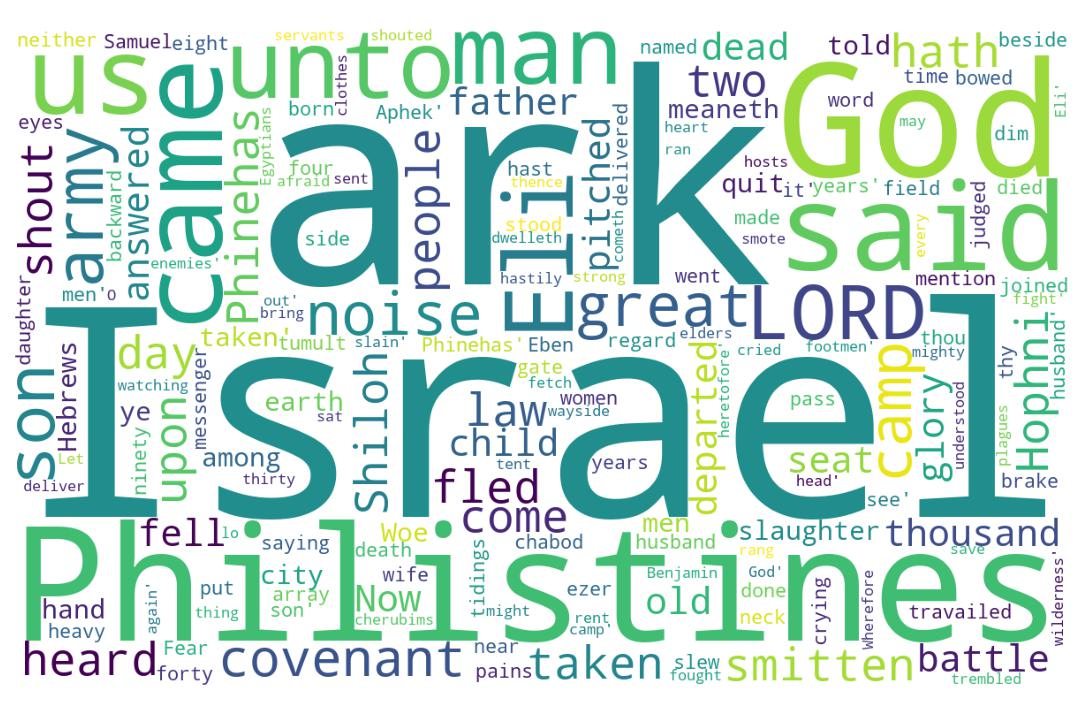
\includegraphics[width=\linewidth]{09OT-1Samuel/1Samuel4-WordCloud.jpg}
  \caption{1 Samuel 4 Word Cloud}
  \label{fig:1 Samuel 4 Word Cloud}
\end{figure}




\marginpar{\scriptsize \centering \fcolorbox{bone}{lime}{\textbf{AN OLD PROBLEM RETURNS}}\\ (1 Samuel 4:1-22) \begin{compactenum}[I.][8]
    \item The \textbf{Conflict}  \index[scripture]{1Samuel!1Sa 04:02}  (1Sa 4:2) 
    \item The \textbf{Context}  Samson's unfinished work in Judges 
    \item Appealing to the \textbf{Covenant}  \index[scripture]{1Samuel!1Sa 04:04}  (1Sa 4:4) 
    \item \textbf{Custody} of the Ark Made no Difference  \index[scripture]{1Samuel!1Sa 04:10}  (1Sa 4:10) 
    \item The \textbf{Cry} of Israel \index[scripture]{1Samuel!1Sa 04:14}  (1Sa 4:14) 
    \item A \textbf{Catastrophe}  \index[scripture]{1Samuel!1Sa 04:17}  (1Sa 4:17) 
    \item A \textbf{Child named Ichabod}  \index[scripture]{1Samuel!1Sa 04:21}  (1Sa 4:21) 
\end{compactenum}}






\footnote{\textcolor[cmyk]{0.99998,1,0,0}{\hyperlink{TOC}{Return to end of Table of Contents.}}}\footnote{\href{https://audiobible.com/bible/1_samuel_4.html}{\textcolor[cmyk]{0.99998,1,0,0}{1 Samuel 4 Audio}}}\textcolor[cmyk]{0.99998,1,0,0}{And the word of Samuel came to all Israel. Now Israel went out against \fcolorbox{bone}{lime}{the} \fcolorbox{bone}{lime}{Philistines} to battle, and pitched beside Eben-ezer: and the Philistines pitched in Aphek.}
[2] \textcolor[cmyk]{0.99998,1,0,0}{And the Philistines put themselves in array against Israel: and when they joined battle, Israel was smitten before the Philistines: and they slew of the army in the field about four thousand men.}
[3] \textcolor[cmyk]{0.99998,1,0,0}{And when the people were come into the camp, the elders of Israel said, Wherefore hath the LORD smitten us to day before the Philistines? Let us fetch the ark of the covenant of the LORD out of Shiloh unto us, that, when it cometh among us, it may save us out of the hand of our enemies.}
[4] \textcolor[cmyk]{0.99998,1,0,0}{So the people sent to Shiloh, that they might bring from thence the \fcolorbox{bone}{lime}{ark of the covenant} of the LORD of hosts, which dwelleth \emph{between} the cherubims: and the two sons of Eli, Hophni and Phinehas, \emph{were} there with the ark of the covenant of God.}
[5] \textcolor[cmyk]{0.99998,1,0,0}{And when the ark of the covenant of the LORD came into the camp, all Israel shouted with a great shout, so that the earth rang again.}
[6] \textcolor[cmyk]{0.99998,1,0,0}{And when the Philistines heard the noise of the shout, they said, What \emph{meaneth} the noise of this great shout in the camp of the Hebrews? And they understood that the ark of the LORD was come into the camp.}
[7] \textcolor[cmyk]{0.99998,1,0,0}{And the Philistines were afraid, for they said, God is come into the camp. And they said, Woe unto us! for there hath not been such a thing heretofore.}
[8] \textcolor[cmyk]{0.99998,1,0,0}{Woe unto us! who shall deliver us out of the hand of these mighty Gods? these \emph{are} the Gods that smote the Egyptians with all the plagues in the wilderness.}
[9] \textcolor[cmyk]{0.99998,1,0,0}{Be strong, and quit yourselves like men, O ye Philistines, that ye be not servants unto the Hebrews, as they have been to you: quit yourselves like men, and fight.}
[10] \textcolor[cmyk]{0.99998,1,0,0}{And the Philistines fought, and \fcolorbox{bone}{lime}{Israel was smitten}, and they fled every man into his tent: and there was a very great slaughter; for there fell of Israel thirty thousand footmen.}
[11] \textcolor[cmyk]{0.99998,1,0,0}{And the ark of God was taken; and the two sons of Eli, Hophni and Phinehas, were slain.}
[12] \textcolor[cmyk]{0.99998,1,0,0}{And there ran a man of Benjamin out of the army, and came to Shiloh the same day with his clothes rent, and with earth upon his head.}
[13] \textcolor[cmyk]{0.99998,1,0,0}{And when he came, lo, Eli sat upon a seat by the wayside watching: for his heart trembled for the ark of God. And when the man came into the city, and told \emph{it}, all the city cried out.}
[14] \textcolor[cmyk]{0.99998,1,0,0}{And when Eli heard the noise of the \fcolorbox{bone}{lime}{crying}, he said, What \emph{meaneth} the noise of this tumult? And the man came in hastily, and told Eli.}
[15] \textcolor[cmyk]{0.99998,1,0,0}{Now Eli was ninety and eight years old; and his eyes were dim, that he could not see.}
[16] \textcolor[cmyk]{0.99998,1,0,0}{And the man said unto Eli, I \emph{am} he that came out of the army, and I fled to day out of the army. And he said, What is there done, my son?}
[17] \textcolor[cmyk]{0.99998,1,0,0}{And the messenger answered and said, Israel is fled before the Philistines, and there hath been also a great \fcolorbox{bone}{lime}{slaughter} among the people, and thy two sons also, Hophni and Phinehas, are dead, and the ark of God is taken.}
[18] \textcolor[cmyk]{0.99998,1,0,0}{And it came to pass, when he made mention of the ark of God, that he fell from off the seat backward by the side of the gate, and his neck brake, and he died: for he was an old man, and heavy. And he had judged Israel forty years.}
[19] \textcolor[cmyk]{0.99998,1,0,0}{And his daughter in law, Phinehas' wife, was with child, \emph{near} to be delivered: and when she heard the tidings that the ark of God was taken, and that her father in law and her husband were dead, she bowed herself and travailed; for her pains came upon her.}
[20] \textcolor[cmyk]{0.99998,1,0,0}{And about the time of her death the women that stood by her said unto her, Fear not; for thou hast born a son. But she answered not, neither did she regard \emph{it}.}
[21] \textcolor[cmyk]{0.99998,1,0,0}{And she named the child I-chabod, saying, The glory is departed from Israel: because the ark of God was taken, and because of her father in law and her husband.}
[22] \textcolor[cmyk]{0.99998,1,0,0}{And she said, The \fcolorbox{bone}{lime}{glory is departed} from Israel: for the ark of God is taken.}
\section{1 Samuel 4 Comments}


%\index[NWIV]{28!1Samuel!1Sa 4:1}\index[AWIP]{And!1Samuel!1Sa 4:1}\index[AWIP]{the!1Samuel!1Sa 4:1}\index[AWIP]{the!1Samuel!1Sa 4:1 (2)}\index[AWIP]{the!1Samuel!1Sa 4:1 (3)}\index[AWIP]{word!1Samuel!1Sa 4:1}\index[AWIP]{of!1Samuel!1Sa 4:1}\index[AWIP]{Samuel!1Samuel!1Sa 4:1}\index[AWIP]{came!1Samuel!1Sa 4:1}\index[AWIP]{to!1Samuel!1Sa 4:1}\index[AWIP]{to!1Samuel!1Sa 4:1 (2)}\index[AWIP]{all!1Samuel!1Sa 4:1}\index[AWIP]{Israel!1Samuel!1Sa 4:1}\index[AWIP]{Israel!1Samuel!1Sa 4:1 (2)}\index[AWIP]{Now!1Samuel!1Sa 4:1}\index[AWIP]{went!1Samuel!1Sa 4:1}\index[AWIP]{out!1Samuel!1Sa 4:1}\index[AWIP]{against!1Samuel!1Sa 4:1}\index[AWIP]{Philistines!1Samuel!1Sa 4:1}\index[AWIP]{Philistines!1Samuel!1Sa 4:1 (2)}\index[AWIP]{battle!1Samuel!1Sa 4:1}\index[AWIP]{and!1Samuel!1Sa 4:1}\index[AWIP]{and!1Samuel!1Sa 4:1 (2)}\index[AWIP]{pitched!1Samuel!1Sa 4:1}\index[AWIP]{pitched!1Samuel!1Sa 4:1 (2)}\index[AWIP]{beside!1Samuel!1Sa 4:1}\index[AWIP]{Eben-ezer!1Samuel!1Sa 4:1}\index[AWIP]{in!1Samuel!1Sa 4:1}\index[AWIP]{Aphek!1Samuel!1Sa 4:1}

\index[NWIV]{33!1Samuel!1Sa 4:2}\index[AWIP]{And!1Samuel!1Sa 4:2}\index[AWIP]{the!1Samuel!1Sa 4:2}\index[AWIP]{the!1Samuel!1Sa 4:2 (2)}\index[AWIP]{the!1Samuel!1Sa 4:2 (3)}\index[AWIP]{the!1Samuel!1Sa 4:2 (4)}\index[AWIP]{Philistines!1Samuel!1Sa 4:2}\index[AWIP]{Philistines!1Samuel!1Sa 4:2 (2)}\index[AWIP]{put!1Samuel!1Sa 4:2}\index[AWIP]{themselves!1Samuel!1Sa 4:2}\index[AWIP]{in!1Samuel!1Sa 4:2}\index[AWIP]{in!1Samuel!1Sa 4:2 (2)}\index[AWIP]{array!1Samuel!1Sa 4:2}\index[AWIP]{against!1Samuel!1Sa 4:2}\index[AWIP]{Israel!1Samuel!1Sa 4:2}\index[AWIP]{Israel!1Samuel!1Sa 4:2 (2)}\index[AWIP]{and!1Samuel!1Sa 4:2}\index[AWIP]{and!1Samuel!1Sa 4:2 (2)}\index[AWIP]{when!1Samuel!1Sa 4:2}\index[AWIP]{they!1Samuel!1Sa 4:2}\index[AWIP]{they!1Samuel!1Sa 4:2 (2)}\index[AWIP]{joined!1Samuel!1Sa 4:2}\index[AWIP]{battle!1Samuel!1Sa 4:2}\index[AWIP]{was!1Samuel!1Sa 4:2}\index[AWIP]{smitten!1Samuel!1Sa 4:2}\index[AWIP]{before!1Samuel!1Sa 4:2}\index[AWIP]{slew!1Samuel!1Sa 4:2}\index[AWIP]{of!1Samuel!1Sa 4:2}\index[AWIP]{army!1Samuel!1Sa 4:2}\index[AWIP]{field!1Samuel!1Sa 4:2}\index[AWIP]{about!1Samuel!1Sa 4:2}\index[AWIP]{four!1Samuel!1Sa 4:2}\index[AWIP]{thousand!1Samuel!1Sa 4:2}\index[AWIP]{men!1Samuel!1Sa 4:2}

\index[NWIV]{58!1Samuel!1Sa 4:3}\index[AWIP]{And!1Samuel!1Sa 4:3}\index[AWIP]{when!1Samuel!1Sa 4:3}\index[AWIP]{when!1Samuel!1Sa 4:3 (2)}\index[AWIP]{the!1Samuel!1Sa 4:3}\index[AWIP]{the!1Samuel!1Sa 4:3 (2)}\index[AWIP]{the!1Samuel!1Sa 4:3 (3)}\index[AWIP]{the!1Samuel!1Sa 4:3 (4)}\index[AWIP]{the!1Samuel!1Sa 4:3 (5)}\index[AWIP]{the!1Samuel!1Sa 4:3 (6)}\index[AWIP]{the!1Samuel!1Sa 4:3 (7)}\index[AWIP]{the!1Samuel!1Sa 4:3 (8)}\index[AWIP]{the!1Samuel!1Sa 4:3 (9)}\index[AWIP]{people!1Samuel!1Sa 4:3}\index[AWIP]{were!1Samuel!1Sa 4:3}\index[AWIP]{come!1Samuel!1Sa 4:3}\index[AWIP]{into!1Samuel!1Sa 4:3}\index[AWIP]{camp!1Samuel!1Sa 4:3}\index[AWIP]{elders!1Samuel!1Sa 4:3}\index[AWIP]{of!1Samuel!1Sa 4:3}\index[AWIP]{of!1Samuel!1Sa 4:3 (2)}\index[AWIP]{of!1Samuel!1Sa 4:3 (3)}\index[AWIP]{of!1Samuel!1Sa 4:3 (4)}\index[AWIP]{of!1Samuel!1Sa 4:3 (5)}\index[AWIP]{of!1Samuel!1Sa 4:3 (6)}\index[AWIP]{Israel!1Samuel!1Sa 4:3}\index[AWIP]{said!1Samuel!1Sa 4:3}\index[AWIP]{Wherefore!1Samuel!1Sa 4:3}\index[AWIP]{hath!1Samuel!1Sa 4:3}\index[AWIP]{LORD!1Samuel!1Sa 4:3}\index[AWIP]{LORD!1Samuel!1Sa 4:3 (2)}\index[AWIP]{smitten!1Samuel!1Sa 4:3}\index[AWIP]{us!1Samuel!1Sa 4:3}\index[AWIP]{us!1Samuel!1Sa 4:3 (2)}\index[AWIP]{us!1Samuel!1Sa 4:3 (3)}\index[AWIP]{us!1Samuel!1Sa 4:3 (4)}\index[AWIP]{us!1Samuel!1Sa 4:3 (5)}\index[AWIP]{to!1Samuel!1Sa 4:3}\index[AWIP]{day!1Samuel!1Sa 4:3}\index[AWIP]{before!1Samuel!1Sa 4:3}\index[AWIP]{Philistines?!1Samuel!1Sa 4:3}\index[AWIP]{Let!1Samuel!1Sa 4:3}\index[AWIP]{fetch!1Samuel!1Sa 4:3}\index[AWIP]{ark!1Samuel!1Sa 4:3}\index[AWIP]{covenant!1Samuel!1Sa 4:3}\index[AWIP]{out!1Samuel!1Sa 4:3}\index[AWIP]{out!1Samuel!1Sa 4:3 (2)}\index[AWIP]{Shiloh!1Samuel!1Sa 4:3}\index[AWIP]{unto!1Samuel!1Sa 4:3}\index[AWIP]{that!1Samuel!1Sa 4:3}\index[AWIP]{it!1Samuel!1Sa 4:3}\index[AWIP]{it!1Samuel!1Sa 4:3 (2)}\index[AWIP]{cometh!1Samuel!1Sa 4:3}\index[AWIP]{among!1Samuel!1Sa 4:3}\index[AWIP]{may!1Samuel!1Sa 4:3}\index[AWIP]{save!1Samuel!1Sa 4:3}\index[AWIP]{hand!1Samuel!1Sa 4:3}\index[AWIP]{our!1Samuel!1Sa 4:3}\index[AWIP]{enemies!1Samuel!1Sa 4:3}

\index[NWIV]{46!1Samuel!1Sa 4:4}\index[AWIP]{So!1Samuel!1Sa 4:4}\index[AWIP]{the!1Samuel!1Sa 4:4}\index[AWIP]{the!1Samuel!1Sa 4:4 (2)}\index[AWIP]{the!1Samuel!1Sa 4:4 (3)}\index[AWIP]{the!1Samuel!1Sa 4:4 (4)}\index[AWIP]{the!1Samuel!1Sa 4:4 (5)}\index[AWIP]{the!1Samuel!1Sa 4:4 (6)}\index[AWIP]{the!1Samuel!1Sa 4:4 (7)}\index[AWIP]{the!1Samuel!1Sa 4:4 (8)}\index[AWIP]{people!1Samuel!1Sa 4:4}\index[AWIP]{sent!1Samuel!1Sa 4:4}\index[AWIP]{to!1Samuel!1Sa 4:4}\index[AWIP]{Shiloh!1Samuel!1Sa 4:4}\index[AWIP]{that!1Samuel!1Sa 4:4}\index[AWIP]{they!1Samuel!1Sa 4:4}\index[AWIP]{might!1Samuel!1Sa 4:4}\index[AWIP]{bring!1Samuel!1Sa 4:4}\index[AWIP]{from!1Samuel!1Sa 4:4}\index[AWIP]{thence!1Samuel!1Sa 4:4}\index[AWIP]{ark!1Samuel!1Sa 4:4}\index[AWIP]{ark!1Samuel!1Sa 4:4 (2)}\index[AWIP]{of!1Samuel!1Sa 4:4}\index[AWIP]{of!1Samuel!1Sa 4:4 (2)}\index[AWIP]{of!1Samuel!1Sa 4:4 (3)}\index[AWIP]{of!1Samuel!1Sa 4:4 (4)}\index[AWIP]{of!1Samuel!1Sa 4:4 (5)}\index[AWIP]{of!1Samuel!1Sa 4:4 (6)}\index[AWIP]{covenant!1Samuel!1Sa 4:4}\index[AWIP]{covenant!1Samuel!1Sa 4:4 (2)}\index[AWIP]{LORD!1Samuel!1Sa 4:4}\index[AWIP]{hosts!1Samuel!1Sa 4:4}\index[AWIP]{which!1Samuel!1Sa 4:4}\index[AWIP]{dwelleth!1Samuel!1Sa 4:4}\index[AWIP]{\emph{between}!1Samuel!1Sa 4:4}\index[AWIP]{cherubims!1Samuel!1Sa 4:4}\index[AWIP]{and!1Samuel!1Sa 4:4}\index[AWIP]{and!1Samuel!1Sa 4:4 (2)}\index[AWIP]{two!1Samuel!1Sa 4:4}\index[AWIP]{sons!1Samuel!1Sa 4:4}\index[AWIP]{Eli!1Samuel!1Sa 4:4}\index[AWIP]{Hophni!1Samuel!1Sa 4:4}\index[AWIP]{Phinehas!1Samuel!1Sa 4:4}\index[AWIP]{\emph{were}!1Samuel!1Sa 4:4}\index[AWIP]{there!1Samuel!1Sa 4:4}\index[AWIP]{with!1Samuel!1Sa 4:4}\index[AWIP]{God!1Samuel!1Sa 4:4}\index[AWIP]{\emph{between}!1Samuel!1Sa 4:4}\index[AWIP]{\emph{were}!1Samuel!1Sa 4:4}

\index[NWIV]{27!1Samuel!1Sa 4:5}\index[AWIP]{And!1Samuel!1Sa 4:5}\index[AWIP]{when!1Samuel!1Sa 4:5}\index[AWIP]{the!1Samuel!1Sa 4:5}\index[AWIP]{the!1Samuel!1Sa 4:5 (2)}\index[AWIP]{the!1Samuel!1Sa 4:5 (3)}\index[AWIP]{the!1Samuel!1Sa 4:5 (4)}\index[AWIP]{the!1Samuel!1Sa 4:5 (5)}\index[AWIP]{ark!1Samuel!1Sa 4:5}\index[AWIP]{of!1Samuel!1Sa 4:5}\index[AWIP]{of!1Samuel!1Sa 4:5 (2)}\index[AWIP]{covenant!1Samuel!1Sa 4:5}\index[AWIP]{LORD!1Samuel!1Sa 4:5}\index[AWIP]{came!1Samuel!1Sa 4:5}\index[AWIP]{into!1Samuel!1Sa 4:5}\index[AWIP]{camp!1Samuel!1Sa 4:5}\index[AWIP]{all!1Samuel!1Sa 4:5}\index[AWIP]{Israel!1Samuel!1Sa 4:5}\index[AWIP]{shouted!1Samuel!1Sa 4:5}\index[AWIP]{with!1Samuel!1Sa 4:5}\index[AWIP]{a!1Samuel!1Sa 4:5}\index[AWIP]{great!1Samuel!1Sa 4:5}\index[AWIP]{shout!1Samuel!1Sa 4:5}\index[AWIP]{so!1Samuel!1Sa 4:5}\index[AWIP]{that!1Samuel!1Sa 4:5}\index[AWIP]{earth!1Samuel!1Sa 4:5}\index[AWIP]{rang!1Samuel!1Sa 4:5}\index[AWIP]{again!1Samuel!1Sa 4:5}

\index[NWIV]{40!1Samuel!1Sa 4:6}\index[AWIP]{And!1Samuel!1Sa 4:6}\index[AWIP]{And!1Samuel!1Sa 4:6 (2)}\index[AWIP]{when!1Samuel!1Sa 4:6}\index[AWIP]{the!1Samuel!1Sa 4:6}\index[AWIP]{the!1Samuel!1Sa 4:6 (2)}\index[AWIP]{the!1Samuel!1Sa 4:6 (3)}\index[AWIP]{the!1Samuel!1Sa 4:6 (4)}\index[AWIP]{the!1Samuel!1Sa 4:6 (5)}\index[AWIP]{the!1Samuel!1Sa 4:6 (6)}\index[AWIP]{the!1Samuel!1Sa 4:6 (7)}\index[AWIP]{the!1Samuel!1Sa 4:6 (8)}\index[AWIP]{the!1Samuel!1Sa 4:6 (9)}\index[AWIP]{Philistines!1Samuel!1Sa 4:6}\index[AWIP]{heard!1Samuel!1Sa 4:6}\index[AWIP]{noise!1Samuel!1Sa 4:6}\index[AWIP]{noise!1Samuel!1Sa 4:6 (2)}\index[AWIP]{of!1Samuel!1Sa 4:6}\index[AWIP]{of!1Samuel!1Sa 4:6 (2)}\index[AWIP]{of!1Samuel!1Sa 4:6 (3)}\index[AWIP]{of!1Samuel!1Sa 4:6 (4)}\index[AWIP]{shout!1Samuel!1Sa 4:6}\index[AWIP]{shout!1Samuel!1Sa 4:6 (2)}\index[AWIP]{they!1Samuel!1Sa 4:6}\index[AWIP]{they!1Samuel!1Sa 4:6 (2)}\index[AWIP]{said!1Samuel!1Sa 4:6}\index[AWIP]{What!1Samuel!1Sa 4:6}\index[AWIP]{\emph{meaneth}!1Samuel!1Sa 4:6}\index[AWIP]{this!1Samuel!1Sa 4:6}\index[AWIP]{great!1Samuel!1Sa 4:6}\index[AWIP]{in!1Samuel!1Sa 4:6}\index[AWIP]{camp!1Samuel!1Sa 4:6}\index[AWIP]{camp!1Samuel!1Sa 4:6 (2)}\index[AWIP]{Hebrews?!1Samuel!1Sa 4:6}\index[AWIP]{understood!1Samuel!1Sa 4:6}\index[AWIP]{that!1Samuel!1Sa 4:6}\index[AWIP]{ark!1Samuel!1Sa 4:6}\index[AWIP]{LORD!1Samuel!1Sa 4:6}\index[AWIP]{was!1Samuel!1Sa 4:6}\index[AWIP]{come!1Samuel!1Sa 4:6}\index[AWIP]{into!1Samuel!1Sa 4:6}\index[AWIP]{\emph{meaneth}!1Samuel!1Sa 4:6}

\index[NWIV]{29!1Samuel!1Sa 4:7}\index[AWIP]{And!1Samuel!1Sa 4:7}\index[AWIP]{And!1Samuel!1Sa 4:7 (2)}\index[AWIP]{the!1Samuel!1Sa 4:7}\index[AWIP]{the!1Samuel!1Sa 4:7 (2)}\index[AWIP]{Philistines!1Samuel!1Sa 4:7}\index[AWIP]{were!1Samuel!1Sa 4:7}\index[AWIP]{afraid!1Samuel!1Sa 4:7}\index[AWIP]{for!1Samuel!1Sa 4:7}\index[AWIP]{for!1Samuel!1Sa 4:7 (2)}\index[AWIP]{they!1Samuel!1Sa 4:7}\index[AWIP]{they!1Samuel!1Sa 4:7 (2)}\index[AWIP]{said!1Samuel!1Sa 4:7}\index[AWIP]{said!1Samuel!1Sa 4:7 (2)}\index[AWIP]{God!1Samuel!1Sa 4:7}\index[AWIP]{is!1Samuel!1Sa 4:7}\index[AWIP]{come!1Samuel!1Sa 4:7}\index[AWIP]{into!1Samuel!1Sa 4:7}\index[AWIP]{camp!1Samuel!1Sa 4:7}\index[AWIP]{Woe!1Samuel!1Sa 4:7}\index[AWIP]{unto!1Samuel!1Sa 4:7}\index[AWIP]{us!!1Samuel!1Sa 4:7}\index[AWIP]{there!1Samuel!1Sa 4:7}\index[AWIP]{hath!1Samuel!1Sa 4:7}\index[AWIP]{not!1Samuel!1Sa 4:7}\index[AWIP]{been!1Samuel!1Sa 4:7}\index[AWIP]{such!1Samuel!1Sa 4:7}\index[AWIP]{a!1Samuel!1Sa 4:7}\index[AWIP]{thing!1Samuel!1Sa 4:7}\index[AWIP]{heretofore!1Samuel!1Sa 4:7}

\index[NWIV]{30!1Samuel!1Sa 4:8}\index[AWIP]{Woe!1Samuel!1Sa 4:8}\index[AWIP]{unto!1Samuel!1Sa 4:8}\index[AWIP]{us!!1Samuel!1Sa 4:8}\index[AWIP]{who!1Samuel!1Sa 4:8}\index[AWIP]{shall!1Samuel!1Sa 4:8}\index[AWIP]{deliver!1Samuel!1Sa 4:8}\index[AWIP]{us!1Samuel!1Sa 4:8}\index[AWIP]{out!1Samuel!1Sa 4:8}\index[AWIP]{of!1Samuel!1Sa 4:8}\index[AWIP]{of!1Samuel!1Sa 4:8 (2)}\index[AWIP]{the!1Samuel!1Sa 4:8}\index[AWIP]{the!1Samuel!1Sa 4:8 (2)}\index[AWIP]{the!1Samuel!1Sa 4:8 (3)}\index[AWIP]{the!1Samuel!1Sa 4:8 (4)}\index[AWIP]{the!1Samuel!1Sa 4:8 (5)}\index[AWIP]{hand!1Samuel!1Sa 4:8}\index[AWIP]{these!1Samuel!1Sa 4:8}\index[AWIP]{these!1Samuel!1Sa 4:8 (2)}\index[AWIP]{mighty!1Samuel!1Sa 4:8}\index[AWIP]{Gods?!1Samuel!1Sa 4:8}\index[AWIP]{\emph{are}!1Samuel!1Sa 4:8}\index[AWIP]{Gods!1Samuel!1Sa 4:8}\index[AWIP]{that!1Samuel!1Sa 4:8}\index[AWIP]{smote!1Samuel!1Sa 4:8}\index[AWIP]{Egyptians!1Samuel!1Sa 4:8}\index[AWIP]{with!1Samuel!1Sa 4:8}\index[AWIP]{all!1Samuel!1Sa 4:8}\index[AWIP]{plagues!1Samuel!1Sa 4:8}\index[AWIP]{in!1Samuel!1Sa 4:8}\index[AWIP]{wilderness!1Samuel!1Sa 4:8}\index[AWIP]{\emph{are}!1Samuel!1Sa 4:8}

\index[NWIV]{30!1Samuel!1Sa 4:9}\index[AWIP]{Be!1Samuel!1Sa 4:9}\index[AWIP]{strong!1Samuel!1Sa 4:9}\index[AWIP]{and!1Samuel!1Sa 4:9}\index[AWIP]{and!1Samuel!1Sa 4:9 (2)}\index[AWIP]{quit!1Samuel!1Sa 4:9}\index[AWIP]{quit!1Samuel!1Sa 4:9 (2)}\index[AWIP]{yourselves!1Samuel!1Sa 4:9}\index[AWIP]{yourselves!1Samuel!1Sa 4:9 (2)}\index[AWIP]{like!1Samuel!1Sa 4:9}\index[AWIP]{like!1Samuel!1Sa 4:9 (2)}\index[AWIP]{men!1Samuel!1Sa 4:9}\index[AWIP]{men!1Samuel!1Sa 4:9 (2)}\index[AWIP]{O!1Samuel!1Sa 4:9}\index[AWIP]{ye!1Samuel!1Sa 4:9}\index[AWIP]{ye!1Samuel!1Sa 4:9 (2)}\index[AWIP]{Philistines!1Samuel!1Sa 4:9}\index[AWIP]{that!1Samuel!1Sa 4:9}\index[AWIP]{be!1Samuel!1Sa 4:9}\index[AWIP]{not!1Samuel!1Sa 4:9}\index[AWIP]{servants!1Samuel!1Sa 4:9}\index[AWIP]{unto!1Samuel!1Sa 4:9}\index[AWIP]{the!1Samuel!1Sa 4:9}\index[AWIP]{Hebrews!1Samuel!1Sa 4:9}\index[AWIP]{as!1Samuel!1Sa 4:9}\index[AWIP]{they!1Samuel!1Sa 4:9}\index[AWIP]{have!1Samuel!1Sa 4:9}\index[AWIP]{been!1Samuel!1Sa 4:9}\index[AWIP]{to!1Samuel!1Sa 4:9}\index[AWIP]{you!1Samuel!1Sa 4:9}\index[AWIP]{fight!1Samuel!1Sa 4:9}

\index[NWIV]{31!1Samuel!1Sa 4:10}\index[AWIP]{And!1Samuel!1Sa 4:10}\index[AWIP]{the!1Samuel!1Sa 4:10}\index[AWIP]{Philistines!1Samuel!1Sa 4:10}\index[AWIP]{fought!1Samuel!1Sa 4:10}\index[AWIP]{and!1Samuel!1Sa 4:10}\index[AWIP]{and!1Samuel!1Sa 4:10 (2)}\index[AWIP]{and!1Samuel!1Sa 4:10 (3)}\index[AWIP]{Israel!1Samuel!1Sa 4:10}\index[AWIP]{Israel!1Samuel!1Sa 4:10 (2)}\index[AWIP]{was!1Samuel!1Sa 4:10}\index[AWIP]{was!1Samuel!1Sa 4:10 (2)}\index[AWIP]{smitten!1Samuel!1Sa 4:10}\index[AWIP]{they!1Samuel!1Sa 4:10}\index[AWIP]{fled!1Samuel!1Sa 4:10}\index[AWIP]{every!1Samuel!1Sa 4:10}\index[AWIP]{man!1Samuel!1Sa 4:10}\index[AWIP]{into!1Samuel!1Sa 4:10}\index[AWIP]{his!1Samuel!1Sa 4:10}\index[AWIP]{tent!1Samuel!1Sa 4:10}\index[AWIP]{there!1Samuel!1Sa 4:10}\index[AWIP]{there!1Samuel!1Sa 4:10 (2)}\index[AWIP]{a!1Samuel!1Sa 4:10}\index[AWIP]{very!1Samuel!1Sa 4:10}\index[AWIP]{great!1Samuel!1Sa 4:10}\index[AWIP]{slaughter!1Samuel!1Sa 4:10}\index[AWIP]{for!1Samuel!1Sa 4:10}\index[AWIP]{fell!1Samuel!1Sa 4:10}\index[AWIP]{of!1Samuel!1Sa 4:10}\index[AWIP]{thirty!1Samuel!1Sa 4:10}\index[AWIP]{thousand!1Samuel!1Sa 4:10}\index[AWIP]{footmen!1Samuel!1Sa 4:10}

\index[NWIV]{18!1Samuel!1Sa 4:11}\index[AWIP]{And!1Samuel!1Sa 4:11}\index[AWIP]{the!1Samuel!1Sa 4:11}\index[AWIP]{the!1Samuel!1Sa 4:11 (2)}\index[AWIP]{ark!1Samuel!1Sa 4:11}\index[AWIP]{of!1Samuel!1Sa 4:11}\index[AWIP]{of!1Samuel!1Sa 4:11 (2)}\index[AWIP]{God!1Samuel!1Sa 4:11}\index[AWIP]{was!1Samuel!1Sa 4:11}\index[AWIP]{taken!1Samuel!1Sa 4:11}\index[AWIP]{and!1Samuel!1Sa 4:11}\index[AWIP]{and!1Samuel!1Sa 4:11 (2)}\index[AWIP]{two!1Samuel!1Sa 4:11}\index[AWIP]{sons!1Samuel!1Sa 4:11}\index[AWIP]{Eli!1Samuel!1Sa 4:11}\index[AWIP]{Hophni!1Samuel!1Sa 4:11}\index[AWIP]{Phinehas!1Samuel!1Sa 4:11}\index[AWIP]{were!1Samuel!1Sa 4:11}\index[AWIP]{slain!1Samuel!1Sa 4:11}

\index[NWIV]{28!1Samuel!1Sa 4:12}\index[AWIP]{And!1Samuel!1Sa 4:12}\index[AWIP]{there!1Samuel!1Sa 4:12}\index[AWIP]{ran!1Samuel!1Sa 4:12}\index[AWIP]{a!1Samuel!1Sa 4:12}\index[AWIP]{man!1Samuel!1Sa 4:12}\index[AWIP]{of!1Samuel!1Sa 4:12}\index[AWIP]{of!1Samuel!1Sa 4:12 (2)}\index[AWIP]{Benjamin!1Samuel!1Sa 4:12}\index[AWIP]{out!1Samuel!1Sa 4:12}\index[AWIP]{the!1Samuel!1Sa 4:12}\index[AWIP]{the!1Samuel!1Sa 4:12 (2)}\index[AWIP]{army!1Samuel!1Sa 4:12}\index[AWIP]{and!1Samuel!1Sa 4:12}\index[AWIP]{and!1Samuel!1Sa 4:12 (2)}\index[AWIP]{came!1Samuel!1Sa 4:12}\index[AWIP]{to!1Samuel!1Sa 4:12}\index[AWIP]{Shiloh!1Samuel!1Sa 4:12}\index[AWIP]{same!1Samuel!1Sa 4:12}\index[AWIP]{day!1Samuel!1Sa 4:12}\index[AWIP]{with!1Samuel!1Sa 4:12}\index[AWIP]{with!1Samuel!1Sa 4:12 (2)}\index[AWIP]{his!1Samuel!1Sa 4:12}\index[AWIP]{his!1Samuel!1Sa 4:12 (2)}\index[AWIP]{clothes!1Samuel!1Sa 4:12}\index[AWIP]{rent!1Samuel!1Sa 4:12}\index[AWIP]{earth!1Samuel!1Sa 4:12}\index[AWIP]{upon!1Samuel!1Sa 4:12}\index[AWIP]{head!1Samuel!1Sa 4:12}

\index[NWIV]{39!1Samuel!1Sa 4:13}\index[AWIP]{And!1Samuel!1Sa 4:13}\index[AWIP]{And!1Samuel!1Sa 4:13 (2)}\index[AWIP]{when!1Samuel!1Sa 4:13}\index[AWIP]{when!1Samuel!1Sa 4:13 (2)}\index[AWIP]{he!1Samuel!1Sa 4:13}\index[AWIP]{came!1Samuel!1Sa 4:13}\index[AWIP]{came!1Samuel!1Sa 4:13 (2)}\index[AWIP]{lo!1Samuel!1Sa 4:13}\index[AWIP]{Eli!1Samuel!1Sa 4:13}\index[AWIP]{sat!1Samuel!1Sa 4:13}\index[AWIP]{upon!1Samuel!1Sa 4:13}\index[AWIP]{a!1Samuel!1Sa 4:13}\index[AWIP]{seat!1Samuel!1Sa 4:13}\index[AWIP]{by!1Samuel!1Sa 4:13}\index[AWIP]{the!1Samuel!1Sa 4:13}\index[AWIP]{the!1Samuel!1Sa 4:13 (2)}\index[AWIP]{the!1Samuel!1Sa 4:13 (3)}\index[AWIP]{the!1Samuel!1Sa 4:13 (4)}\index[AWIP]{the!1Samuel!1Sa 4:13 (5)}\index[AWIP]{wayside!1Samuel!1Sa 4:13}\index[AWIP]{watching!1Samuel!1Sa 4:13}\index[AWIP]{for!1Samuel!1Sa 4:13}\index[AWIP]{for!1Samuel!1Sa 4:13 (2)}\index[AWIP]{his!1Samuel!1Sa 4:13}\index[AWIP]{heart!1Samuel!1Sa 4:13}\index[AWIP]{trembled!1Samuel!1Sa 4:13}\index[AWIP]{ark!1Samuel!1Sa 4:13}\index[AWIP]{of!1Samuel!1Sa 4:13}\index[AWIP]{God!1Samuel!1Sa 4:13}\index[AWIP]{man!1Samuel!1Sa 4:13}\index[AWIP]{into!1Samuel!1Sa 4:13}\index[AWIP]{city!1Samuel!1Sa 4:13}\index[AWIP]{city!1Samuel!1Sa 4:13 (2)}\index[AWIP]{and!1Samuel!1Sa 4:13}\index[AWIP]{told!1Samuel!1Sa 4:13}\index[AWIP]{\emph{it}!1Samuel!1Sa 4:13}\index[AWIP]{all!1Samuel!1Sa 4:13}\index[AWIP]{cried!1Samuel!1Sa 4:13}\index[AWIP]{out!1Samuel!1Sa 4:13}\index[AWIP]{\emph{it}!1Samuel!1Sa 4:13}

\index[NWIV]{27!1Samuel!1Sa 4:14}\index[AWIP]{And!1Samuel!1Sa 4:14}\index[AWIP]{And!1Samuel!1Sa 4:14 (2)}\index[AWIP]{when!1Samuel!1Sa 4:14}\index[AWIP]{Eli!1Samuel!1Sa 4:14}\index[AWIP]{Eli!1Samuel!1Sa 4:14 (2)}\index[AWIP]{heard!1Samuel!1Sa 4:14}\index[AWIP]{the!1Samuel!1Sa 4:14}\index[AWIP]{the!1Samuel!1Sa 4:14 (2)}\index[AWIP]{the!1Samuel!1Sa 4:14 (3)}\index[AWIP]{the!1Samuel!1Sa 4:14 (4)}\index[AWIP]{noise!1Samuel!1Sa 4:14}\index[AWIP]{noise!1Samuel!1Sa 4:14 (2)}\index[AWIP]{of!1Samuel!1Sa 4:14}\index[AWIP]{of!1Samuel!1Sa 4:14 (2)}\index[AWIP]{crying!1Samuel!1Sa 4:14}\index[AWIP]{he!1Samuel!1Sa 4:14}\index[AWIP]{said!1Samuel!1Sa 4:14}\index[AWIP]{What!1Samuel!1Sa 4:14}\index[AWIP]{\emph{meaneth}!1Samuel!1Sa 4:14}\index[AWIP]{this!1Samuel!1Sa 4:14}\index[AWIP]{tumult?!1Samuel!1Sa 4:14}\index[AWIP]{man!1Samuel!1Sa 4:14}\index[AWIP]{came!1Samuel!1Sa 4:14}\index[AWIP]{in!1Samuel!1Sa 4:14}\index[AWIP]{hastily!1Samuel!1Sa 4:14}\index[AWIP]{and!1Samuel!1Sa 4:14}\index[AWIP]{told!1Samuel!1Sa 4:14}\index[AWIP]{\emph{meaneth}!1Samuel!1Sa 4:14}

\index[NWIV]{18!1Samuel!1Sa 4:15}\index[AWIP]{Now!1Samuel!1Sa 4:15}\index[AWIP]{Eli!1Samuel!1Sa 4:15}\index[AWIP]{was!1Samuel!1Sa 4:15}\index[AWIP]{ninety!1Samuel!1Sa 4:15}\index[AWIP]{and!1Samuel!1Sa 4:15}\index[AWIP]{and!1Samuel!1Sa 4:15 (2)}\index[AWIP]{eight!1Samuel!1Sa 4:15}\index[AWIP]{years!1Samuel!1Sa 4:15}\index[AWIP]{old!1Samuel!1Sa 4:15}\index[AWIP]{his!1Samuel!1Sa 4:15}\index[AWIP]{eyes!1Samuel!1Sa 4:15}\index[AWIP]{were!1Samuel!1Sa 4:15}\index[AWIP]{dim!1Samuel!1Sa 4:15}\index[AWIP]{that!1Samuel!1Sa 4:15}\index[AWIP]{he!1Samuel!1Sa 4:15}\index[AWIP]{could!1Samuel!1Sa 4:15}\index[AWIP]{not!1Samuel!1Sa 4:15}\index[AWIP]{see!1Samuel!1Sa 4:15}

\index[NWIV]{33!1Samuel!1Sa 4:16}\index[AWIP]{And!1Samuel!1Sa 4:16}\index[AWIP]{And!1Samuel!1Sa 4:16 (2)}\index[AWIP]{the!1Samuel!1Sa 4:16}\index[AWIP]{the!1Samuel!1Sa 4:16 (2)}\index[AWIP]{the!1Samuel!1Sa 4:16 (3)}\index[AWIP]{man!1Samuel!1Sa 4:16}\index[AWIP]{said!1Samuel!1Sa 4:16}\index[AWIP]{said!1Samuel!1Sa 4:16 (2)}\index[AWIP]{unto!1Samuel!1Sa 4:16}\index[AWIP]{Eli!1Samuel!1Sa 4:16}\index[AWIP]{I!1Samuel!1Sa 4:16}\index[AWIP]{I!1Samuel!1Sa 4:16 (2)}\index[AWIP]{\emph{am}!1Samuel!1Sa 4:16}\index[AWIP]{he!1Samuel!1Sa 4:16}\index[AWIP]{he!1Samuel!1Sa 4:16 (2)}\index[AWIP]{that!1Samuel!1Sa 4:16}\index[AWIP]{came!1Samuel!1Sa 4:16}\index[AWIP]{out!1Samuel!1Sa 4:16}\index[AWIP]{out!1Samuel!1Sa 4:16 (2)}\index[AWIP]{of!1Samuel!1Sa 4:16}\index[AWIP]{of!1Samuel!1Sa 4:16 (2)}\index[AWIP]{army!1Samuel!1Sa 4:16}\index[AWIP]{army!1Samuel!1Sa 4:16 (2)}\index[AWIP]{and!1Samuel!1Sa 4:16}\index[AWIP]{fled!1Samuel!1Sa 4:16}\index[AWIP]{to!1Samuel!1Sa 4:16}\index[AWIP]{day!1Samuel!1Sa 4:16}\index[AWIP]{What!1Samuel!1Sa 4:16}\index[AWIP]{is!1Samuel!1Sa 4:16}\index[AWIP]{there!1Samuel!1Sa 4:16}\index[AWIP]{done!1Samuel!1Sa 4:16}\index[AWIP]{my!1Samuel!1Sa 4:16}\index[AWIP]{son?!1Samuel!1Sa 4:16}\index[AWIP]{\emph{am}!1Samuel!1Sa 4:16}

\index[NWIV]{40!1Samuel!1Sa 4:17}\index[AWIP]{And!1Samuel!1Sa 4:17}\index[AWIP]{the!1Samuel!1Sa 4:17}\index[AWIP]{the!1Samuel!1Sa 4:17 (2)}\index[AWIP]{the!1Samuel!1Sa 4:17 (3)}\index[AWIP]{the!1Samuel!1Sa 4:17 (4)}\index[AWIP]{messenger!1Samuel!1Sa 4:17}\index[AWIP]{answered!1Samuel!1Sa 4:17}\index[AWIP]{and!1Samuel!1Sa 4:17}\index[AWIP]{and!1Samuel!1Sa 4:17 (2)}\index[AWIP]{and!1Samuel!1Sa 4:17 (3)}\index[AWIP]{and!1Samuel!1Sa 4:17 (4)}\index[AWIP]{and!1Samuel!1Sa 4:17 (5)}\index[AWIP]{said!1Samuel!1Sa 4:17}\index[AWIP]{Israel!1Samuel!1Sa 4:17}\index[AWIP]{is!1Samuel!1Sa 4:17}\index[AWIP]{is!1Samuel!1Sa 4:17 (2)}\index[AWIP]{fled!1Samuel!1Sa 4:17}\index[AWIP]{before!1Samuel!1Sa 4:17}\index[AWIP]{Philistines!1Samuel!1Sa 4:17}\index[AWIP]{there!1Samuel!1Sa 4:17}\index[AWIP]{hath!1Samuel!1Sa 4:17}\index[AWIP]{been!1Samuel!1Sa 4:17}\index[AWIP]{also!1Samuel!1Sa 4:17}\index[AWIP]{also!1Samuel!1Sa 4:17 (2)}\index[AWIP]{a!1Samuel!1Sa 4:17}\index[AWIP]{great!1Samuel!1Sa 4:17}\index[AWIP]{slaughter!1Samuel!1Sa 4:17}\index[AWIP]{among!1Samuel!1Sa 4:17}\index[AWIP]{people!1Samuel!1Sa 4:17}\index[AWIP]{thy!1Samuel!1Sa 4:17}\index[AWIP]{two!1Samuel!1Sa 4:17}\index[AWIP]{sons!1Samuel!1Sa 4:17}\index[AWIP]{Hophni!1Samuel!1Sa 4:17}\index[AWIP]{Phinehas!1Samuel!1Sa 4:17}\index[AWIP]{are!1Samuel!1Sa 4:17}\index[AWIP]{dead!1Samuel!1Sa 4:17}\index[AWIP]{ark!1Samuel!1Sa 4:17}\index[AWIP]{of!1Samuel!1Sa 4:17}\index[AWIP]{God!1Samuel!1Sa 4:17}\index[AWIP]{taken!1Samuel!1Sa 4:17}

\index[NWIV]{50!1Samuel!1Sa 4:18}\index[AWIP]{And!1Samuel!1Sa 4:18}\index[AWIP]{And!1Samuel!1Sa 4:18 (2)}\index[AWIP]{it!1Samuel!1Sa 4:18}\index[AWIP]{came!1Samuel!1Sa 4:18}\index[AWIP]{to!1Samuel!1Sa 4:18}\index[AWIP]{pass!1Samuel!1Sa 4:18}\index[AWIP]{when!1Samuel!1Sa 4:18}\index[AWIP]{he!1Samuel!1Sa 4:18}\index[AWIP]{he!1Samuel!1Sa 4:18 (2)}\index[AWIP]{he!1Samuel!1Sa 4:18 (3)}\index[AWIP]{he!1Samuel!1Sa 4:18 (4)}\index[AWIP]{he!1Samuel!1Sa 4:18 (5)}\index[AWIP]{made!1Samuel!1Sa 4:18}\index[AWIP]{mention!1Samuel!1Sa 4:18}\index[AWIP]{of!1Samuel!1Sa 4:18}\index[AWIP]{of!1Samuel!1Sa 4:18 (2)}\index[AWIP]{of!1Samuel!1Sa 4:18 (3)}\index[AWIP]{the!1Samuel!1Sa 4:18}\index[AWIP]{the!1Samuel!1Sa 4:18 (2)}\index[AWIP]{the!1Samuel!1Sa 4:18 (3)}\index[AWIP]{the!1Samuel!1Sa 4:18 (4)}\index[AWIP]{ark!1Samuel!1Sa 4:18}\index[AWIP]{God!1Samuel!1Sa 4:18}\index[AWIP]{that!1Samuel!1Sa 4:18}\index[AWIP]{fell!1Samuel!1Sa 4:18}\index[AWIP]{from!1Samuel!1Sa 4:18}\index[AWIP]{off!1Samuel!1Sa 4:18}\index[AWIP]{seat!1Samuel!1Sa 4:18}\index[AWIP]{backward!1Samuel!1Sa 4:18}\index[AWIP]{by!1Samuel!1Sa 4:18}\index[AWIP]{side!1Samuel!1Sa 4:18}\index[AWIP]{gate!1Samuel!1Sa 4:18}\index[AWIP]{and!1Samuel!1Sa 4:18}\index[AWIP]{and!1Samuel!1Sa 4:18 (2)}\index[AWIP]{and!1Samuel!1Sa 4:18 (3)}\index[AWIP]{his!1Samuel!1Sa 4:18}\index[AWIP]{neck!1Samuel!1Sa 4:18}\index[AWIP]{brake!1Samuel!1Sa 4:18}\index[AWIP]{died!1Samuel!1Sa 4:18}\index[AWIP]{for!1Samuel!1Sa 4:18}\index[AWIP]{was!1Samuel!1Sa 4:18}\index[AWIP]{an!1Samuel!1Sa 4:18}\index[AWIP]{old!1Samuel!1Sa 4:18}\index[AWIP]{man!1Samuel!1Sa 4:18}\index[AWIP]{heavy!1Samuel!1Sa 4:18}\index[AWIP]{had!1Samuel!1Sa 4:18}\index[AWIP]{judged!1Samuel!1Sa 4:18}\index[AWIP]{Israel!1Samuel!1Sa 4:18}\index[AWIP]{forty!1Samuel!1Sa 4:18}\index[AWIP]{years!1Samuel!1Sa 4:18}

\index[NWIV]{49!1Samuel!1Sa 4:19}\index[AWIP]{And!1Samuel!1Sa 4:19}\index[AWIP]{his!1Samuel!1Sa 4:19}\index[AWIP]{daughter!1Samuel!1Sa 4:19}\index[AWIP]{in!1Samuel!1Sa 4:19}\index[AWIP]{in!1Samuel!1Sa 4:19 (2)}\index[AWIP]{law!1Samuel!1Sa 4:19}\index[AWIP]{law!1Samuel!1Sa 4:19 (2)}\index[AWIP]{Phinehas'!1Samuel!1Sa 4:19}\index[AWIP]{wife!1Samuel!1Sa 4:19}\index[AWIP]{was!1Samuel!1Sa 4:19}\index[AWIP]{was!1Samuel!1Sa 4:19 (2)}\index[AWIP]{with!1Samuel!1Sa 4:19}\index[AWIP]{child!1Samuel!1Sa 4:19}\index[AWIP]{\emph{near}!1Samuel!1Sa 4:19}\index[AWIP]{to!1Samuel!1Sa 4:19}\index[AWIP]{be!1Samuel!1Sa 4:19}\index[AWIP]{delivered!1Samuel!1Sa 4:19}\index[AWIP]{and!1Samuel!1Sa 4:19}\index[AWIP]{and!1Samuel!1Sa 4:19 (2)}\index[AWIP]{and!1Samuel!1Sa 4:19 (3)}\index[AWIP]{and!1Samuel!1Sa 4:19 (4)}\index[AWIP]{when!1Samuel!1Sa 4:19}\index[AWIP]{she!1Samuel!1Sa 4:19}\index[AWIP]{she!1Samuel!1Sa 4:19 (2)}\index[AWIP]{heard!1Samuel!1Sa 4:19}\index[AWIP]{the!1Samuel!1Sa 4:19}\index[AWIP]{the!1Samuel!1Sa 4:19 (2)}\index[AWIP]{tidings!1Samuel!1Sa 4:19}\index[AWIP]{that!1Samuel!1Sa 4:19}\index[AWIP]{that!1Samuel!1Sa 4:19 (2)}\index[AWIP]{ark!1Samuel!1Sa 4:19}\index[AWIP]{of!1Samuel!1Sa 4:19}\index[AWIP]{God!1Samuel!1Sa 4:19}\index[AWIP]{taken!1Samuel!1Sa 4:19}\index[AWIP]{her!1Samuel!1Sa 4:19}\index[AWIP]{her!1Samuel!1Sa 4:19 (2)}\index[AWIP]{her!1Samuel!1Sa 4:19 (3)}\index[AWIP]{her!1Samuel!1Sa 4:19 (4)}\index[AWIP]{father!1Samuel!1Sa 4:19}\index[AWIP]{husband!1Samuel!1Sa 4:19}\index[AWIP]{were!1Samuel!1Sa 4:19}\index[AWIP]{dead!1Samuel!1Sa 4:19}\index[AWIP]{bowed!1Samuel!1Sa 4:19}\index[AWIP]{herself!1Samuel!1Sa 4:19}\index[AWIP]{travailed!1Samuel!1Sa 4:19}\index[AWIP]{for!1Samuel!1Sa 4:19}\index[AWIP]{pains!1Samuel!1Sa 4:19}\index[AWIP]{came!1Samuel!1Sa 4:19}\index[AWIP]{upon!1Samuel!1Sa 4:19}\index[AWIP]{\emph{near}!1Samuel!1Sa 4:19}

\index[NWIV]{33!1Samuel!1Sa 4:20}\index[AWIP]{And!1Samuel!1Sa 4:20}\index[AWIP]{about!1Samuel!1Sa 4:20}\index[AWIP]{the!1Samuel!1Sa 4:20}\index[AWIP]{the!1Samuel!1Sa 4:20 (2)}\index[AWIP]{time!1Samuel!1Sa 4:20}\index[AWIP]{of!1Samuel!1Sa 4:20}\index[AWIP]{her!1Samuel!1Sa 4:20}\index[AWIP]{her!1Samuel!1Sa 4:20 (2)}\index[AWIP]{her!1Samuel!1Sa 4:20 (3)}\index[AWIP]{death!1Samuel!1Sa 4:20}\index[AWIP]{women!1Samuel!1Sa 4:20}\index[AWIP]{that!1Samuel!1Sa 4:20}\index[AWIP]{stood!1Samuel!1Sa 4:20}\index[AWIP]{by!1Samuel!1Sa 4:20}\index[AWIP]{said!1Samuel!1Sa 4:20}\index[AWIP]{unto!1Samuel!1Sa 4:20}\index[AWIP]{Fear!1Samuel!1Sa 4:20}\index[AWIP]{not!1Samuel!1Sa 4:20}\index[AWIP]{not!1Samuel!1Sa 4:20 (2)}\index[AWIP]{for!1Samuel!1Sa 4:20}\index[AWIP]{thou!1Samuel!1Sa 4:20}\index[AWIP]{hast!1Samuel!1Sa 4:20}\index[AWIP]{born!1Samuel!1Sa 4:20}\index[AWIP]{a!1Samuel!1Sa 4:20}\index[AWIP]{son!1Samuel!1Sa 4:20}\index[AWIP]{But!1Samuel!1Sa 4:20}\index[AWIP]{she!1Samuel!1Sa 4:20}\index[AWIP]{she!1Samuel!1Sa 4:20 (2)}\index[AWIP]{answered!1Samuel!1Sa 4:20}\index[AWIP]{neither!1Samuel!1Sa 4:20}\index[AWIP]{did!1Samuel!1Sa 4:20}\index[AWIP]{regard!1Samuel!1Sa 4:20}\index[AWIP]{\emph{it}!1Samuel!1Sa 4:20}\index[AWIP]{\emph{it}!1Samuel!1Sa 4:20}

\index[NWIV]{30!1Samuel!1Sa 4:21}\index[AWIP]{And!1Samuel!1Sa 4:21}\index[AWIP]{she!1Samuel!1Sa 4:21}\index[AWIP]{named!1Samuel!1Sa 4:21}\index[AWIP]{the!1Samuel!1Sa 4:21}\index[AWIP]{the!1Samuel!1Sa 4:21 (2)}\index[AWIP]{child!1Samuel!1Sa 4:21}\index[AWIP]{I-chabod!1Samuel!1Sa 4:21}\index[AWIP]{saying!1Samuel!1Sa 4:21}\index[AWIP]{The!1Samuel!1Sa 4:21}\index[AWIP]{glory!1Samuel!1Sa 4:21}\index[AWIP]{is!1Samuel!1Sa 4:21}\index[AWIP]{departed!1Samuel!1Sa 4:21}\index[AWIP]{from!1Samuel!1Sa 4:21}\index[AWIP]{Israel!1Samuel!1Sa 4:21}\index[AWIP]{because!1Samuel!1Sa 4:21}\index[AWIP]{because!1Samuel!1Sa 4:21 (2)}\index[AWIP]{ark!1Samuel!1Sa 4:21}\index[AWIP]{of!1Samuel!1Sa 4:21}\index[AWIP]{of!1Samuel!1Sa 4:21 (2)}\index[AWIP]{God!1Samuel!1Sa 4:21}\index[AWIP]{was!1Samuel!1Sa 4:21}\index[AWIP]{taken!1Samuel!1Sa 4:21}\index[AWIP]{and!1Samuel!1Sa 4:21}\index[AWIP]{and!1Samuel!1Sa 4:21 (2)}\index[AWIP]{her!1Samuel!1Sa 4:21}\index[AWIP]{her!1Samuel!1Sa 4:21 (2)}\index[AWIP]{father!1Samuel!1Sa 4:21}\index[AWIP]{in!1Samuel!1Sa 4:21}\index[AWIP]{law!1Samuel!1Sa 4:21}\index[AWIP]{husband!1Samuel!1Sa 4:21}

\index[NWIV]{16!1Samuel!1Sa 4:22}\index[AWIP]{And!1Samuel!1Sa 4:22}\index[AWIP]{she!1Samuel!1Sa 4:22}\index[AWIP]{said!1Samuel!1Sa 4:22}\index[AWIP]{The!1Samuel!1Sa 4:22}\index[AWIP]{glory!1Samuel!1Sa 4:22}\index[AWIP]{is!1Samuel!1Sa 4:22}\index[AWIP]{is!1Samuel!1Sa 4:22 (2)}\index[AWIP]{departed!1Samuel!1Sa 4:22}\index[AWIP]{from!1Samuel!1Sa 4:22}\index[AWIP]{Israel!1Samuel!1Sa 4:22}\index[AWIP]{for!1Samuel!1Sa 4:22}\index[AWIP]{the!1Samuel!1Sa 4:22}\index[AWIP]{ark!1Samuel!1Sa 4:22}\index[AWIP]{of!1Samuel!1Sa 4:22}\index[AWIP]{God!1Samuel!1Sa 4:22}\index[AWIP]{taken!1Samuel!1Sa 4:22}


\section{1 Samuel 4 Outlines}

\subsection{My Outlines}

\subsubsection{An Old Problem Returns}
\index[speaker]{Keith Anthony!1 Samuel 04 (An Old Problem Returns)}
\index[series]{1 Samuel (Keith Anthony)!1 Samuel 04 (An Old Problem Returns)}
\index[date]{2018/03/24!1 Samuel 04 (An Old Problem Returns) (Keith Anthony)}

\begin{compactenum}[I.][7]
    \item The \textbf{Conflict}  \index[scripture]{1Samuel!1Sa 04:02}  (1Sa 4:2) 
    \item The \textbf{Context}  Samson's unfinished work in Judges 
    \item Appealing to the \textbf{Covenant}  \index[scripture]{1Samuel!1Sa 04:04}  (1Sa 4:4) 
    \item \textbf{Custody} of the Ark Made no Difference  \index[scripture]{1Samuel!1Sa 04:10}  (1Sa 4:10) 
    \item The \textbf{Cry} of Israel \index[scripture]{1Samuel!1Sa 04:14}  (1Sa 4:14) 
    \item A \textbf{Catastrophe}  \index[scripture]{1Samuel!1Sa 04:17}  (1Sa4:17) 
    \item A \textbf{Child named Ichabod}  \index[scripture]{1Samuel!1Sa 04:21}  (1Sa 4:21) 
\end{compactenum} 


\subsection{My Outlines from Others}


%\\section{1 Samuel 4 Statistics}

%%%%%%%%%%%%%%%%%%%%%%%%%%%
%%%%% Word Statistics
%%%%%%%%%%%%%%%%%%%%%%%%%%


\normalsize



\subsection{Chapter Word Statistics}


%%%%%%%%%%
%%%%%%%%%%
 
\begin{center}
\begin{longtable}{l|c|c|c|c}
\caption[Stats for 1 Samuel 4]{Stats for 1 Samuel 4} \label{table:Stats for 1 Samuel 4} \\ 
\hline \multicolumn{1}{|c|}{\textbf{Verse(s)}} & \multicolumn{1}{|c|}{\textbf{Count}} & \multicolumn{1}{|c|}{\textbf{Unique}} & \multicolumn{1}{|c|}{\textbf{Italics}} & \multicolumn{1}{|c|}{\textbf{Uniq Italic}}  \\ \hline 
\endfirsthead
 
\multicolumn{5}{c}
{{\bfseries \tablename\ \thetable{} -- continued from previous page}} \\  
\hline \multicolumn{1}{|c|}{\textbf{Verse(s)}} & \multicolumn{1}{|c|}{\textbf{Count}} & \multicolumn{1}{|c|}{\textbf{Unique}} & \multicolumn{1}{|c|}{\textbf{Italics}} & \multicolumn{1}{|c|}{\textbf{Uniq Italic}}  \\ \hline 
\endhead
 
\hline \multicolumn{5}{|r|}{{Continued if needed}} \\ \hline
\endfoot 
1 & 28 & 21 & 0 & 0\\ \hline
2 & 33 & 25 & 0 & 0\\ \hline
3 & 58 & 37 & 0 & 0\\ \hline
4 & 46 & 31 & 2 & 2\\ \hline
5 & 27 & 22 & 0 & 0\\ \hline
6 & 40 & 24 & 1 & 1\\ \hline
7 & 29 & 24 & 0 & 0\\ \hline
8 & 30 & 22 & 1 & 1\\ \hline
9 & 30 & 24 & 0 & 0\\ \hline
10 & 31 & 26 & 0 & 0\\ \hline
11 & 18 & 15 & 0 & 0\\ \hline
12 & 28 & 23 & 0 & 0\\ \hline
13 & 39 & 30 & 1 & 1\\ \hline
14 & 27 & 20 & 1 & 1\\ \hline
15 & 18 & 17 & 0 & 0\\ \hline
16 & 33 & 24 & 1 & 1\\ \hline
17 & 40 & 31 & 0 & 0\\ \hline
18 & 50 & 38 & 0 & 0\\ \hline
19 & 49 & 37 & 1 & 1\\ \hline
20 & 33 & 28 & 1 & 1\\ \hline
21 & 30 & 25 & 0 & 0\\ \hline
22 & 16 & 15 & 0 & 0\\ \hline
\hline \hline
Total & 733 & 237 & 9 & 7



\end{longtable}
\end{center}

%%%%%%%%%%
%%%%%%%%%%
 
\subsection{Words by Frequency}

\begin{center}
\begin{longtable}{l|r}
\caption[Word Frequencies in FirstSamuel 4]{Word Frequencies in FirstSamuel 4} \label{table:WordsIn-FirstSamuel-4} \\ 
\hline \multicolumn{1}{|c|}{\textbf{Word}} & \multicolumn{1}{c|}{\textbf{Frequency}} \\ \hline 
\endfirsthead
 
\multicolumn{2}{c}
{{\bfseries \tablename\ \thetable{} -- continued from previous page}} \\ 
\hline \multicolumn{1}{|c|}{\textbf{Word}} & \multicolumn{1}{c|}{\textbf{Frequency}} \\ \hline 
\endhead
 
\hline \multicolumn{2}{|r|}{{Continued if needed}} \\ \hline
\endfoot
 
\hline \hline
\endlastfoot
the & 78 \\ \hline
of & 41 \\ \hline
and & 34 \\ \hline
And & 24 \\ \hline
Israel & 12 \\ \hline
ark & 12 \\ \hline
that & 12 \\ \hline
Philistines & 10 \\ \hline
when & 10 \\ \hline
was & 10 \\ \hline
said & 10 \\ \hline
he & 10 \\ \hline
came & 9 \\ \hline
to & 9 \\ \hline
in & 9 \\ \hline
they & 9 \\ \hline
God & 9 \\ \hline
for & 9 \\ \hline
her & 9 \\ \hline
out & 8 \\ \hline
us & 8 \\ \hline
Eli & 7 \\ \hline
there & 7 \\ \hline
a & 7 \\ \hline
is & 7 \\ \hline
his & 7 \\ \hline
into & 6 \\ \hline
unto & 6 \\ \hline
with & 6 \\ \hline
man & 6 \\ \hline
she & 6 \\ \hline
were & 5 \\ \hline
camp & 5 \\ \hline
LORD & 5 \\ \hline
not & 5 \\ \hline
taken & 5 \\ \hline
all & 4 \\ \hline
army & 4 \\ \hline
covenant & 4 \\ \hline
from & 4 \\ \hline
great & 4 \\ \hline
noise & 4 \\ \hline
smitten & 3 \\ \hline
before & 3 \\ \hline
men & 3 \\ \hline
people & 3 \\ \hline
come & 3 \\ \hline
hath & 3 \\ \hline
day & 3 \\ \hline
Shiloh & 3 \\ \hline
it & 3 \\ \hline
two & 3 \\ \hline
sons & 3 \\ \hline
Hophni & 3 \\ \hline
Phinehas & 3 \\ \hline
shout & 3 \\ \hline
heard & 3 \\ \hline
What & 3 \\ \hline
been & 3 \\ \hline
fled & 3 \\ \hline
upon & 3 \\ \hline
by & 3 \\ \hline
law & 3 \\ \hline
Now & 2 \\ \hline
against & 2 \\ \hline
battle & 2 \\ \hline
pitched & 2 \\ \hline
about & 2 \\ \hline
thousand & 2 \\ \hline
among & 2 \\ \hline
hand & 2 \\ \hline
earth & 2 \\ \hline
\emph{meaneth} & 2 \\ \hline
this & 2 \\ \hline
Hebrews & 2 \\ \hline
Woe & 2 \\ \hline
these & 2 \\ \hline
Gods & 2 \\ \hline
quit & 2 \\ \hline
yourselves & 2 \\ \hline
like & 2 \\ \hline
ye & 2 \\ \hline
be & 2 \\ \hline
slaughter & 2 \\ \hline
fell & 2 \\ \hline
seat & 2 \\ \hline
city & 2 \\ \hline
told & 2 \\ \hline
\emph{it} & 2 \\ \hline
years & 2 \\ \hline
old & 2 \\ \hline
I & 2 \\ \hline
son & 2 \\ \hline
answered & 2 \\ \hline
also & 2 \\ \hline
dead & 2 \\ \hline
child & 2 \\ \hline
father & 2 \\ \hline
husband & 2 \\ \hline
The & 2 \\ \hline
glory & 2 \\ \hline
departed & 2 \\ \hline
because & 2 \\ \hline
word & 1 \\ \hline
Samuel & 1 \\ \hline
went & 1 \\ \hline
beside & 1 \\ \hline
Eben-ezer & 1 \\ \hline
Aphek & 1 \\ \hline
put & 1 \\ \hline
themselves & 1 \\ \hline
array & 1 \\ \hline
joined & 1 \\ \hline
slew & 1 \\ \hline
field & 1 \\ \hline
four & 1 \\ \hline
elders & 1 \\ \hline
Wherefore & 1 \\ \hline
Let & 1 \\ \hline
fetch & 1 \\ \hline
cometh & 1 \\ \hline
may & 1 \\ \hline
save & 1 \\ \hline
our & 1 \\ \hline
enemies & 1 \\ \hline
So & 1 \\ \hline
sent & 1 \\ \hline
might & 1 \\ \hline
bring & 1 \\ \hline
thence & 1 \\ \hline
hosts & 1 \\ \hline
which & 1 \\ \hline
dwelleth & 1 \\ \hline
\emph{between} & 1 \\ \hline
cherubims & 1 \\ \hline
\emph{were} & 1 \\ \hline
shouted & 1 \\ \hline
so & 1 \\ \hline
rang & 1 \\ \hline
again & 1 \\ \hline
understood & 1 \\ \hline
afraid & 1 \\ \hline
such & 1 \\ \hline
thing & 1 \\ \hline
heretofore & 1 \\ \hline
who & 1 \\ \hline
shall & 1 \\ \hline
deliver & 1 \\ \hline
mighty & 1 \\ \hline
\emph{are} & 1 \\ \hline
smote & 1 \\ \hline
Egyptians & 1 \\ \hline
plagues & 1 \\ \hline
wilderness & 1 \\ \hline
Be & 1 \\ \hline
strong & 1 \\ \hline
O & 1 \\ \hline
servants & 1 \\ \hline
as & 1 \\ \hline
have & 1 \\ \hline
you & 1 \\ \hline
fight & 1 \\ \hline
fought & 1 \\ \hline
every & 1 \\ \hline
tent & 1 \\ \hline
very & 1 \\ \hline
thirty & 1 \\ \hline
footmen & 1 \\ \hline
slain & 1 \\ \hline
ran & 1 \\ \hline
Benjamin & 1 \\ \hline
same & 1 \\ \hline
clothes & 1 \\ \hline
rent & 1 \\ \hline
head & 1 \\ \hline
lo & 1 \\ \hline
sat & 1 \\ \hline
wayside & 1 \\ \hline
watching & 1 \\ \hline
heart & 1 \\ \hline
trembled & 1 \\ \hline
cried & 1 \\ \hline
crying & 1 \\ \hline
tumult & 1 \\ \hline
hastily & 1 \\ \hline
ninety & 1 \\ \hline
eight & 1 \\ \hline
eyes & 1 \\ \hline
dim & 1 \\ \hline
could & 1 \\ \hline
see & 1 \\ \hline
\emph{am} & 1 \\ \hline
done & 1 \\ \hline
my & 1 \\ \hline
messenger & 1 \\ \hline
thy & 1 \\ \hline
are & 1 \\ \hline
pass & 1 \\ \hline
made & 1 \\ \hline
mention & 1 \\ \hline
off & 1 \\ \hline
backward & 1 \\ \hline
side & 1 \\ \hline
gate & 1 \\ \hline
neck & 1 \\ \hline
brake & 1 \\ \hline
died & 1 \\ \hline
an & 1 \\ \hline
heavy & 1 \\ \hline
had & 1 \\ \hline
judged & 1 \\ \hline
forty & 1 \\ \hline
daughter & 1 \\ \hline
Phinehas' & 1 \\ \hline
wife & 1 \\ \hline
\emph{near} & 1 \\ \hline
delivered & 1 \\ \hline
tidings & 1 \\ \hline
bowed & 1 \\ \hline
herself & 1 \\ \hline
travailed & 1 \\ \hline
pains & 1 \\ \hline
time & 1 \\ \hline
death & 1 \\ \hline
women & 1 \\ \hline
stood & 1 \\ \hline
Fear & 1 \\ \hline
thou & 1 \\ \hline
hast & 1 \\ \hline
born & 1 \\ \hline
But & 1 \\ \hline
neither & 1 \\ \hline
did & 1 \\ \hline
regard & 1 \\ \hline
named & 1 \\ \hline
I-chabod & 1 \\ \hline
saying & 1 \\ \hline
\end{longtable}
\end{center}



\normalsize



\subsection{Words Alphabetically}

\begin{center}
\begin{longtable}{l|r}
\caption[Word Alphabetically in 1 Samuel 4]{Word Alphabetically in 1 Samuel 4} \label{table:WordsIn-1 Samuel-4} \\ 
\hline \multicolumn{1}{|c|}{\textbf{Word}} & \multicolumn{1}{c|}{\textbf{Frequency}} \\ \hline 
\endfirsthead
 
\multicolumn{2}{c}
{{\bfseries \tablename\ \thetable{} -- continued from previous page}} \\ 
\hline \multicolumn{1}{|c|}{\textbf{Word}} & \multicolumn{1}{c|}{\textbf{Frequency}} \\ \hline 
\endhead
 
\hline \multicolumn{2}{|r|}{{Continued if needed}} \\ \hline
\endfoot
 
\hline \hline
\endlastfoot
And & 24 \\ \hline
Aphek & 1 \\ \hline
Be & 1 \\ \hline
Benjamin & 1 \\ \hline
But & 1 \\ \hline
Eben-ezer & 1 \\ \hline
Egyptians & 1 \\ \hline
Eli & 7 \\ \hline
Fear & 1 \\ \hline
God & 9 \\ \hline
Gods & 2 \\ \hline
Hebrews & 2 \\ \hline
Hophni & 3 \\ \hline
I & 2 \\ \hline
I-chabod & 1 \\ \hline
Israel & 12 \\ \hline
LORD & 5 \\ \hline
Let & 1 \\ \hline
Now & 2 \\ \hline
O & 1 \\ \hline
Philistines & 10 \\ \hline
Phinehas & 3 \\ \hline
Phinehas' & 1 \\ \hline
Samuel & 1 \\ \hline
Shiloh & 3 \\ \hline
So & 1 \\ \hline
The & 2 \\ \hline
What & 3 \\ \hline
Wherefore & 1 \\ \hline
Woe & 2 \\ \hline
\emph{am} & 1 \\ \hline
\emph{are} & 1 \\ \hline
\emph{between} & 1 \\ \hline
\emph{it} & 2 \\ \hline
\emph{meaneth} & 2 \\ \hline
\emph{near} & 1 \\ \hline
\emph{were} & 1 \\ \hline
a & 7 \\ \hline
about & 2 \\ \hline
afraid & 1 \\ \hline
again & 1 \\ \hline
against & 2 \\ \hline
all & 4 \\ \hline
also & 2 \\ \hline
among & 2 \\ \hline
an & 1 \\ \hline
and & 34 \\ \hline
answered & 2 \\ \hline
are & 1 \\ \hline
ark & 12 \\ \hline
army & 4 \\ \hline
array & 1 \\ \hline
as & 1 \\ \hline
backward & 1 \\ \hline
battle & 2 \\ \hline
be & 2 \\ \hline
because & 2 \\ \hline
been & 3 \\ \hline
before & 3 \\ \hline
beside & 1 \\ \hline
born & 1 \\ \hline
bowed & 1 \\ \hline
brake & 1 \\ \hline
bring & 1 \\ \hline
by & 3 \\ \hline
came & 9 \\ \hline
camp & 5 \\ \hline
cherubims & 1 \\ \hline
child & 2 \\ \hline
city & 2 \\ \hline
clothes & 1 \\ \hline
come & 3 \\ \hline
cometh & 1 \\ \hline
could & 1 \\ \hline
covenant & 4 \\ \hline
cried & 1 \\ \hline
crying & 1 \\ \hline
daughter & 1 \\ \hline
day & 3 \\ \hline
dead & 2 \\ \hline
death & 1 \\ \hline
deliver & 1 \\ \hline
delivered & 1 \\ \hline
departed & 2 \\ \hline
did & 1 \\ \hline
died & 1 \\ \hline
dim & 1 \\ \hline
done & 1 \\ \hline
dwelleth & 1 \\ \hline
earth & 2 \\ \hline
eight & 1 \\ \hline
elders & 1 \\ \hline
enemies & 1 \\ \hline
every & 1 \\ \hline
eyes & 1 \\ \hline
father & 2 \\ \hline
fell & 2 \\ \hline
fetch & 1 \\ \hline
field & 1 \\ \hline
fight & 1 \\ \hline
fled & 3 \\ \hline
footmen & 1 \\ \hline
for & 9 \\ \hline
forty & 1 \\ \hline
fought & 1 \\ \hline
four & 1 \\ \hline
from & 4 \\ \hline
gate & 1 \\ \hline
glory & 2 \\ \hline
great & 4 \\ \hline
had & 1 \\ \hline
hand & 2 \\ \hline
hast & 1 \\ \hline
hastily & 1 \\ \hline
hath & 3 \\ \hline
have & 1 \\ \hline
he & 10 \\ \hline
head & 1 \\ \hline
heard & 3 \\ \hline
heart & 1 \\ \hline
heavy & 1 \\ \hline
her & 9 \\ \hline
heretofore & 1 \\ \hline
herself & 1 \\ \hline
his & 7 \\ \hline
hosts & 1 \\ \hline
husband & 2 \\ \hline
in & 9 \\ \hline
into & 6 \\ \hline
is & 7 \\ \hline
it & 3 \\ \hline
joined & 1 \\ \hline
judged & 1 \\ \hline
law & 3 \\ \hline
like & 2 \\ \hline
lo & 1 \\ \hline
made & 1 \\ \hline
man & 6 \\ \hline
may & 1 \\ \hline
men & 3 \\ \hline
mention & 1 \\ \hline
messenger & 1 \\ \hline
might & 1 \\ \hline
mighty & 1 \\ \hline
my & 1 \\ \hline
named & 1 \\ \hline
neck & 1 \\ \hline
neither & 1 \\ \hline
ninety & 1 \\ \hline
noise & 4 \\ \hline
not & 5 \\ \hline
of & 41 \\ \hline
off & 1 \\ \hline
old & 2 \\ \hline
our & 1 \\ \hline
out & 8 \\ \hline
pains & 1 \\ \hline
pass & 1 \\ \hline
people & 3 \\ \hline
pitched & 2 \\ \hline
plagues & 1 \\ \hline
put & 1 \\ \hline
quit & 2 \\ \hline
ran & 1 \\ \hline
rang & 1 \\ \hline
regard & 1 \\ \hline
rent & 1 \\ \hline
said & 10 \\ \hline
same & 1 \\ \hline
sat & 1 \\ \hline
save & 1 \\ \hline
saying & 1 \\ \hline
seat & 2 \\ \hline
see & 1 \\ \hline
sent & 1 \\ \hline
servants & 1 \\ \hline
shall & 1 \\ \hline
she & 6 \\ \hline
shout & 3 \\ \hline
shouted & 1 \\ \hline
side & 1 \\ \hline
slain & 1 \\ \hline
slaughter & 2 \\ \hline
slew & 1 \\ \hline
smitten & 3 \\ \hline
smote & 1 \\ \hline
so & 1 \\ \hline
son & 2 \\ \hline
sons & 3 \\ \hline
stood & 1 \\ \hline
strong & 1 \\ \hline
such & 1 \\ \hline
taken & 5 \\ \hline
tent & 1 \\ \hline
that & 12 \\ \hline
the & 78 \\ \hline
themselves & 1 \\ \hline
thence & 1 \\ \hline
there & 7 \\ \hline
these & 2 \\ \hline
they & 9 \\ \hline
thing & 1 \\ \hline
thirty & 1 \\ \hline
this & 2 \\ \hline
thou & 1 \\ \hline
thousand & 2 \\ \hline
thy & 1 \\ \hline
tidings & 1 \\ \hline
time & 1 \\ \hline
to & 9 \\ \hline
told & 2 \\ \hline
travailed & 1 \\ \hline
trembled & 1 \\ \hline
tumult & 1 \\ \hline
two & 3 \\ \hline
understood & 1 \\ \hline
unto & 6 \\ \hline
upon & 3 \\ \hline
us & 8 \\ \hline
very & 1 \\ \hline
was & 10 \\ \hline
watching & 1 \\ \hline
wayside & 1 \\ \hline
went & 1 \\ \hline
were & 5 \\ \hline
when & 10 \\ \hline
which & 1 \\ \hline
who & 1 \\ \hline
wife & 1 \\ \hline
wilderness & 1 \\ \hline
with & 6 \\ \hline
women & 1 \\ \hline
word & 1 \\ \hline
ye & 2 \\ \hline
years & 2 \\ \hline
you & 1 \\ \hline
yourselves & 2 \\ \hline
\end{longtable}
\end{center}



\normalsize



\subsection{Word Lengths in Chapter}
\normalsize
\begin{longtable}{l|p{3.75in}}
\caption[Words by Length in 1 Samuel 4]{Words by Length in 1 Samuel 4} \label{table:WordsIn-1 Samuel-4} \\ 
\hline \multicolumn{1}{|c|}{\textbf{Length}} & \multicolumn{1}{c|}{\textbf{Words}} \\ \hline 
\endfirsthead
 
\multicolumn{2}{c}
{{\bfseries \tablename\ \thetable{} -- continued from previous page}} \\ 
\hline \multicolumn{1}{|c|}{\textbf{Length}} & \multicolumn{1}{c|}{\textbf{Words}} \\ \hline 
\endhead
 
\hline \multicolumn{2}{|r|}{{Continued if needed}} \\ \hline
\endfoot
 
\hline \hline
\endlastfoot
1 & a, O, I \\ \hline
2 & of, to, in, us, it, So, so, is, Be, ye, be, as, he, lo, by, \emph{it}, \emph{am}, my, an \\ \hline
3 & And, the, all, Now, out, and, put, was, men, day, Let, ark, may, our, two, Eli, God, for, Woe, not, who, \emph{are}, you, man, his, ran, sat, old, dim, see, son, thy, are, off, had, law, she, her, But, did, The \\ \hline
4 & word, came, went, when, they, slew, army, four, were, come, into, camp, said, hath, LORD, unto, that, save, hand, sent, from, sons, \emph{were}, with, rang, What, this, been, such, Gods, quit, like, have, fled, tent, very, fell, same, rent, upon, head, seat, city, told, eyes, done, also, dead, pass, made, side, gate, neck, died, wife, \emph{near}, time, Fear, thou, hast, born \\ \hline
5 & Aphek, array, field, about, fetch, among, might, bring, hosts, which, there, great, shout, earth, again, heard, noise, thing, shall, these, smote, fight, every, taken, slain, heart, cried, eight, years, could, brake, heavy, forty, child, bowed, pains, death, women, stood, named, glory \\ \hline
6 & Samuel, Israel, battle, beside, joined, before, people, elders, Shiloh, cometh, thence, Hophni, afraid, mighty, strong, fought, thirty, crying, tumult, ninety, judged, father, regard, saying \\ \hline
7 & against, pitched, smitten, enemies, \emph{between}, shouted, \emph{meaneth}, Hebrews, deliver, plagues, footmen, clothes, wayside, hastily, mention, tidings, husband, herself, neither, because \\ \hline
8 & thousand, covenant, dwelleth, Phinehas, servants, Benjamin, watching, trembled, answered, backward, daughter, I-chabod, departed \\ \hline
9 & Eben-ezer, Wherefore, cherubims, Egyptians, slaughter, messenger, Phinehas', delivered, travailed \\ \hline
10 & themselves, understood, heretofore, wilderness, yourselves \\ \hline
11 & Philistines \\ \hline
\end{longtable}






%%%%%%%%%%
%%%%%%%%%%
 



%%%%%%%%%%
%%%%%%%%%%
\subsection{Verses with 18 Words in Chapter}
\normalsize
\begin{longtable}{l|p{3.75in}}
\caption[Verses with 18 Words  in 1 Samuel 4]{Verses with 18 Words  in 1 amuel 4} \label{table:Verses with 18 Words in-1 amuel-4} \\ 
\hline \multicolumn{1}{|c|}{\textbf{Reference}} & \multicolumn{1}{c|}{\textbf{Verse}} \\ \hline 
\endfirsthead
 
\multicolumn{2}{c}
{{\bfseries \tablename\ \thetable{} -- continued from previous page}} \\ 
\hline \multicolumn{1}{|c|}{\textbf{Reference}} & \multicolumn{1}{c|}{\textbf{Verse}} \\ \hline 
\endhead
 
\hline \multicolumn{2}{|r|}{{Continued if needed}} \\ \hline
\endfoot
 
\hline \hline
\endlastfoot
1Samuel 04:11 & And the ark of God was taken; and the two sons of Eli, Hophni and Phinehas, were slain. \\ \hline
1Samuel 04:15 & Now Eli was ninety and eight years old; and his eyes were dim, that he could not see. \\ \hline
\end{longtable}






%%%%%%%%%%
%%%%%%%%%%
\subsection{1Samuel 4 Repeated Phrases}


%%%%%%%%%%
%%%%%%%%%%
\normalsize
 
\begin{center}
\begin{longtable}{|p{3.0in}|p{0.5in}|}
\caption[1Samuel 4 Repeated Phrases]{1Samuel 4 Repeated Phrases}\label{table:Repeated Phrases 1Samuel 4} \\
\hline \multicolumn{1}{|c|}{\textbf{Phrase}} & \multicolumn{1}{c|}{\textbf{Frequency}} \\ \hline 
\endfirsthead
 
\multicolumn{2}{c}
{{\bfseries \tablename\ \thetable{} -- continued from previous page}} \\  
\hline \multicolumn{1}{|c|}{\textbf{Phrase}} & \multicolumn{1}{c|}{\textbf{Frequency}} \\ \hline 
\endhead
 
\hline \multicolumn{2}{c}{{ }} \\ \hline
\endfoot 
of the & 19\\ \hline 
the ark & 12\\ \hline 
the ark of & 12\\ \hline 
ark of & 12\\ \hline 
the Philistines & 9\\ \hline 
And the & 8\\ \hline 
of God & 8\\ \hline 
the ark of God & 7\\ \hline 
ark of God & 7\\ \hline 
And when & 6\\ \hline 
out of & 6\\ \hline 
into the & 5\\ \hline 
the camp & 5\\ \hline 
the LORD & 5\\ \hline 
the ark of the & 5\\ \hline 
ark of the & 5\\ \hline 
out of the & 5\\ \hline 
and the & 4\\ \hline 
of the army & 4\\ \hline 
the army & 4\\ \hline 
And when the & 4\\ \hline 
when the & 4\\ \hline 
into the camp & 4\\ \hline 
the ark of the covenant & 4\\ \hline 
the ark of the covenant of & 4\\ \hline 
ark of the covenant & 4\\ \hline 
ark of the covenant of & 4\\ \hline 
of the covenant & 4\\ \hline 
of the covenant of & 4\\ \hline 
the covenant & 4\\ \hline 
the covenant of & 4\\ \hline 
covenant of & 4\\ \hline 
of the LORD & 4\\ \hline 
the noise & 4\\ \hline 
the noise of & 4\\ \hline 
noise of & 4\\ \hline 
came to & 3\\ \hline 
And the Philistines & 3\\ \hline 
before the & 3\\ \hline 
before the Philistines & 3\\ \hline 
in the & 3\\ \hline 
the people & 3\\ \hline 
come into & 3\\ \hline 
come into the & 3\\ \hline 
come into the camp & 3\\ \hline 
the ark of the covenant of the & 3\\ \hline 
the ark of the covenant of the LORD & 3\\ \hline 
ark of the covenant of the & 3\\ \hline 
ark of the covenant of the LORD & 3\\ \hline 
of the covenant of the & 3\\ \hline 
of the covenant of the LORD & 3\\ \hline 
the covenant of the & 3\\ \hline 
the covenant of the LORD & 3\\ \hline 
covenant of the & 3\\ \hline 
covenant of the LORD & 3\\ \hline 
unto us & 3\\ \hline 
two sons & 3\\ \hline 
Hophni and & 3\\ \hline 
Hophni and Phinehas & 3\\ \hline 
and Phinehas & 3\\ \hline 
that the & 3\\ \hline 
heard the & 3\\ \hline 
they said & 3\\ \hline 
said What & 3\\ \hline 
God is & 3\\ \hline 
the ark of God was & 3\\ \hline 
the ark of God was taken & 3\\ \hline 
the ark of God was taken and & 3\\ \hline 
ark of God was & 3\\ \hline 
ark of God was taken & 3\\ \hline 
ark of God was taken and & 3\\ \hline 
of God was & 3\\ \hline 
of God was taken & 3\\ \hline 
of God was taken and & 3\\ \hline 
God was & 3\\ \hline 
God was taken & 3\\ \hline 
God was taken and & 3\\ \hline 
was taken & 3\\ \hline 
was taken and & 3\\ \hline 
taken and & 3\\ \hline 
out of the army & 3\\ \hline 
the man & 3\\ \hline 
in law & 3\\ \hline 
\end{longtable}
\end{center}



%%%%%%%%%%
%%%%%%%%%%




\chapter{1 Samuel 5}

\begin{figure}
  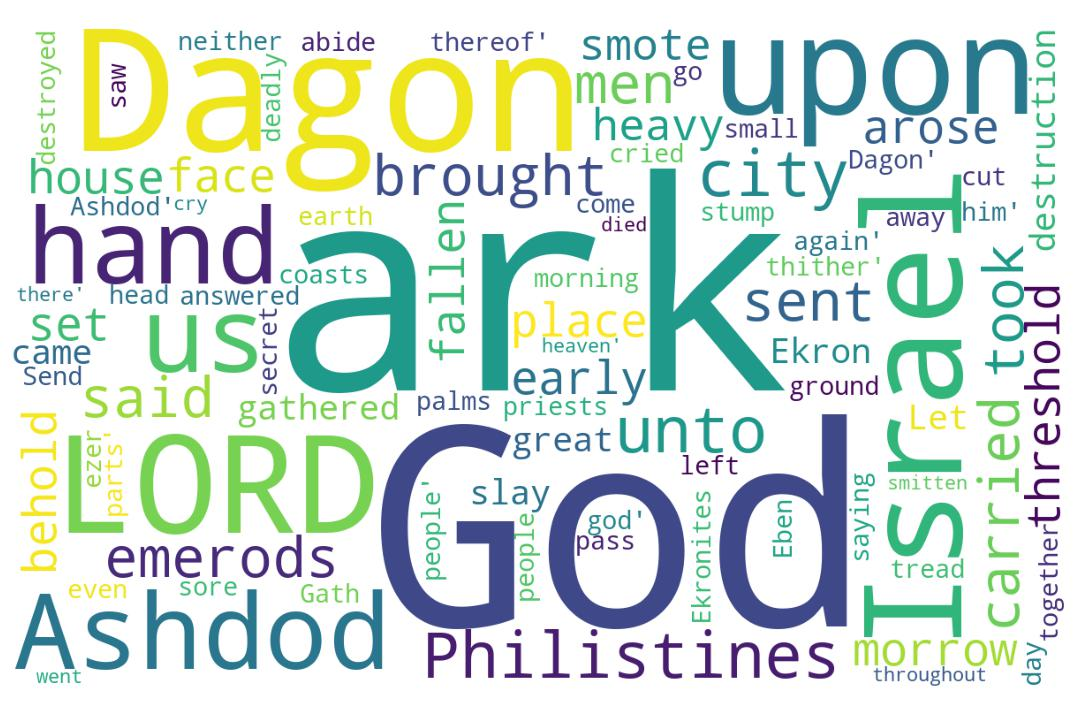
\includegraphics[width=\linewidth]{09OT-1Samuel/1Samuel5-WordCloud.jpg}
  \caption{1 Samuel 5 Word Cloud}
  \label{fig:1 Samuel 5 Word Cloud}
\end{figure}

\marginpar{\scriptsize \centering \fcolorbox{bone}{lime}{\textbf{LIVING WITH THE ARK}}\\ (1 Samuel 5:1-12) \begin{compactenum}[I.][8]
    \item \textbf{Unsuspecting People}  \index[scripture]{1Samuel!1Sa 05:01}  (1Sa5:1) 
    \item An \textbf{Uncommon Place}  \index[scripture]{1Samuel!1Sa 05:02}  (1Sa 5:2) 
    \item An \textbf{Unmanageable Presence}  \index[scripture]{1Samuel!1Sa 05:03}  (1Sa 5:3) 
    \item An \textbf{Undeniable Power}  \index[scripture]{1Samuel!1Sa 05:04}  (1Sa 5:4 
    \item An \textbf{Uncomfortable Problem}  \index[scripture]{1Samuel!1Sa 05:09}  (1Sa 5:9) 
    \item An \textbf{Unremitting Pain}  \index[scripture]{1Samuel!1Sa 05:12}  (1Sa 5:12) 
    \item \textbf{Unmistakeable Points}  %\index[scripture]{1Samuel!1Sa 05:12}  (1Sa 5:12) 
\end{compactenum}}






\footnote{\textcolor[cmyk]{0.99998,1,0,0}{\hyperlink{TOC}{Return to end of Table of Contents.}}}\footnote{\href{https://audiobible.com/bible/1_samuel_5.html}{\textcolor[cmyk]{0.99998,1,0,0}{1 Samuel 5 Audio}}}\textcolor[cmyk]{0.99998,1,0,0}{And the Philistines took the ark of God, and brought it from Eben-ezer unto Ashdod.}
[2] \textcolor[cmyk]{0.99998,1,0,0}{When the Philistines \fcolorbox{bone}{lime}{took the ark of God}, they brought it into the house of Dagon, and \fcolorbox{bone}{lime}{set it by Dagon}.}\\
\\
\P \textcolor[cmyk]{0.99998,1,0,0}{And when they of Ashdod arose early on the morrow, behold, \fcolorbox{bone}{lime}{Dagon} \fcolorbox{bone}{lime}{\emph{was} fallen} upon his face to the earth before the ark of the LORD. And they took Dagon, and set him in his place again.}
[4] \textcolor[cmyk]{0.99998,1,0,0}{And when they arose early on the morrow morning, behold, Dagon \emph{was} fallen upon his face to the ground before the ark of the LORD; and the head of Dagon and both the palms of his hands \emph{were} \fcolorbox{bone}{lime}{cut off} upon the threshold; only \emph{the} \emph{stump} \emph{of} Dagon was left to him.}
[5] \textcolor[cmyk]{0.99998,1,0,0}{Therefore neither the priests of Dagon, nor any that come into Dagon's house, tread on the threshold of Dagon in Ashdod unto this day.}
[6] \textcolor[cmyk]{0.99998,1,0,0}{But the hand of the LORD was heavy upon them of Ashdod, and he destroyed them, and smote them with emerods, \emph{even} Ashdod and the coasts thereof.}
[7] \textcolor[cmyk]{0.99998,1,0,0}{And when the men of Ashdod saw that \emph{it} \emph{was} so, they said, The ark of the God of Israel shall not abide with us: for his hand is sore upon us, and upon Dagon our god.}
[8] \textcolor[cmyk]{0.99998,1,0,0}{They sent therefore and gathered all the lords of the Philistines unto them, and said, What shall we do with the ark of the God of Israel? And they answered, Let the ark of the God of Israel be carried about unto Gath. And they carried the ark of the God of Israel about \emph{thither}.}
[9] \textcolor[cmyk]{0.99998,1,0,0}{And it was \emph{so}, that, after they had carried it about, the hand of the LORD was against the city with a very great \fcolorbox{bone}{lime}{destruction}: and he smote the men of the city, both small and great, and they had \fcolorbox{bone}{lime}{emerods} in their secret parts.}\\
\\
\P \textcolor[cmyk]{0.99998,1,0,0}{Therefore they sent the ark of God to Ekron. And it came to pass, as the ark of God came to Ekron, that the Ekronites cried out, saying, They have brought about the ark of the God of Israel to us, to slay us and our people.}
[11] \textcolor[cmyk]{0.99998,1,0,0}{So they sent and gathered together all the lords of the Philistines, and said, Send away the ark of the God of Israel, and let it go again to his own place, that it slay us not, and our people: for there was a deadly destruction throughout all the city; the hand of God was very heavy there.}
[12] \textcolor[cmyk]{0.99998,1,0,0}{And the men that died not were smitten with the emerods: and the \fcolorbox{bone}{lime}{cry of the city} went up to heaven.}
\section{1 Samuel 5 Comments}


%\index[NWIV]{15!1Samuel!1Sa 5:1}\index[AWIP]{And!1Samuel!1Sa 5:1}\index[AWIP]{the!1Samuel!1Sa 5:1}\index[AWIP]{the!1Samuel!1Sa 5:1 (2)}\index[AWIP]{Philistines!1Samuel!1Sa 5:1}\index[AWIP]{took!1Samuel!1Sa 5:1}\index[AWIP]{ark!1Samuel!1Sa 5:1}\index[AWIP]{of!1Samuel!1Sa 5:1}\index[AWIP]{God!1Samuel!1Sa 5:1}\index[AWIP]{and!1Samuel!1Sa 5:1}\index[AWIP]{brought!1Samuel!1Sa 5:1}\index[AWIP]{it!1Samuel!1Sa 5:1}\index[AWIP]{from!1Samuel!1Sa 5:1}\index[AWIP]{Eben-ezer!1Samuel!1Sa 5:1}\index[AWIP]{unto!1Samuel!1Sa 5:1}\index[AWIP]{Ashdod!1Samuel!1Sa 5:1}

\index[NWIV]{21!1Samuel!1Sa 5:2}\index[AWIP]{When!1Samuel!1Sa 5:2}\index[AWIP]{the!1Samuel!1Sa 5:2}\index[AWIP]{the!1Samuel!1Sa 5:2 (2)}\index[AWIP]{the!1Samuel!1Sa 5:2 (3)}\index[AWIP]{Philistines!1Samuel!1Sa 5:2}\index[AWIP]{took!1Samuel!1Sa 5:2}\index[AWIP]{ark!1Samuel!1Sa 5:2}\index[AWIP]{of!1Samuel!1Sa 5:2}\index[AWIP]{of!1Samuel!1Sa 5:2 (2)}\index[AWIP]{God!1Samuel!1Sa 5:2}\index[AWIP]{they!1Samuel!1Sa 5:2}\index[AWIP]{brought!1Samuel!1Sa 5:2}\index[AWIP]{it!1Samuel!1Sa 5:2}\index[AWIP]{it!1Samuel!1Sa 5:2 (2)}\index[AWIP]{into!1Samuel!1Sa 5:2}\index[AWIP]{house!1Samuel!1Sa 5:2}\index[AWIP]{Dagon!1Samuel!1Sa 5:2}\index[AWIP]{Dagon!1Samuel!1Sa 5:2 (2)}\index[AWIP]{and!1Samuel!1Sa 5:2}\index[AWIP]{set!1Samuel!1Sa 5:2}\index[AWIP]{by!1Samuel!1Sa 5:2}

\index[NWIV]{37!1Samuel!1Sa 5:3}\index[AWIP]{And!1Samuel!1Sa 5:3}\index[AWIP]{And!1Samuel!1Sa 5:3 (2)}\index[AWIP]{when!1Samuel!1Sa 5:3}\index[AWIP]{they!1Samuel!1Sa 5:3}\index[AWIP]{they!1Samuel!1Sa 5:3 (2)}\index[AWIP]{of!1Samuel!1Sa 5:3}\index[AWIP]{of!1Samuel!1Sa 5:3 (2)}\index[AWIP]{Ashdod!1Samuel!1Sa 5:3}\index[AWIP]{arose!1Samuel!1Sa 5:3}\index[AWIP]{early!1Samuel!1Sa 5:3}\index[AWIP]{on!1Samuel!1Sa 5:3}\index[AWIP]{the!1Samuel!1Sa 5:3}\index[AWIP]{the!1Samuel!1Sa 5:3 (2)}\index[AWIP]{the!1Samuel!1Sa 5:3 (3)}\index[AWIP]{the!1Samuel!1Sa 5:3 (4)}\index[AWIP]{morrow!1Samuel!1Sa 5:3}\index[AWIP]{behold!1Samuel!1Sa 5:3}\index[AWIP]{Dagon!1Samuel!1Sa 5:3}\index[AWIP]{Dagon!1Samuel!1Sa 5:3 (2)}\index[AWIP]{\emph{was}!1Samuel!1Sa 5:3}\index[AWIP]{fallen!1Samuel!1Sa 5:3}\index[AWIP]{upon!1Samuel!1Sa 5:3}\index[AWIP]{his!1Samuel!1Sa 5:3}\index[AWIP]{his!1Samuel!1Sa 5:3 (2)}\index[AWIP]{face!1Samuel!1Sa 5:3}\index[AWIP]{to!1Samuel!1Sa 5:3}\index[AWIP]{earth!1Samuel!1Sa 5:3}\index[AWIP]{before!1Samuel!1Sa 5:3}\index[AWIP]{ark!1Samuel!1Sa 5:3}\index[AWIP]{LORD!1Samuel!1Sa 5:3}\index[AWIP]{took!1Samuel!1Sa 5:3}\index[AWIP]{and!1Samuel!1Sa 5:3}\index[AWIP]{set!1Samuel!1Sa 5:3}\index[AWIP]{him!1Samuel!1Sa 5:3}\index[AWIP]{in!1Samuel!1Sa 5:3}\index[AWIP]{place!1Samuel!1Sa 5:3}\index[AWIP]{again!1Samuel!1Sa 5:3}\index[AWIP]{\emph{was}!1Samuel!1Sa 5:3}

\index[NWIV]{52!1Samuel!1Sa 5:4}\index[AWIP]{And!1Samuel!1Sa 5:4}\index[AWIP]{when!1Samuel!1Sa 5:4}\index[AWIP]{they!1Samuel!1Sa 5:4}\index[AWIP]{arose!1Samuel!1Sa 5:4}\index[AWIP]{early!1Samuel!1Sa 5:4}\index[AWIP]{on!1Samuel!1Sa 5:4}\index[AWIP]{the!1Samuel!1Sa 5:4}\index[AWIP]{the!1Samuel!1Sa 5:4 (2)}\index[AWIP]{the!1Samuel!1Sa 5:4 (3)}\index[AWIP]{the!1Samuel!1Sa 5:4 (4)}\index[AWIP]{the!1Samuel!1Sa 5:4 (5)}\index[AWIP]{the!1Samuel!1Sa 5:4 (6)}\index[AWIP]{the!1Samuel!1Sa 5:4 (7)}\index[AWIP]{morrow!1Samuel!1Sa 5:4}\index[AWIP]{morning!1Samuel!1Sa 5:4}\index[AWIP]{behold!1Samuel!1Sa 5:4}\index[AWIP]{Dagon!1Samuel!1Sa 5:4}\index[AWIP]{Dagon!1Samuel!1Sa 5:4 (2)}\index[AWIP]{Dagon!1Samuel!1Sa 5:4 (3)}\index[AWIP]{\emph{was}!1Samuel!1Sa 5:4}\index[AWIP]{fallen!1Samuel!1Sa 5:4}\index[AWIP]{upon!1Samuel!1Sa 5:4}\index[AWIP]{upon!1Samuel!1Sa 5:4 (2)}\index[AWIP]{his!1Samuel!1Sa 5:4}\index[AWIP]{his!1Samuel!1Sa 5:4 (2)}\index[AWIP]{face!1Samuel!1Sa 5:4}\index[AWIP]{to!1Samuel!1Sa 5:4}\index[AWIP]{to!1Samuel!1Sa 5:4 (2)}\index[AWIP]{ground!1Samuel!1Sa 5:4}\index[AWIP]{before!1Samuel!1Sa 5:4}\index[AWIP]{ark!1Samuel!1Sa 5:4}\index[AWIP]{of!1Samuel!1Sa 5:4}\index[AWIP]{of!1Samuel!1Sa 5:4 (2)}\index[AWIP]{of!1Samuel!1Sa 5:4 (3)}\index[AWIP]{LORD!1Samuel!1Sa 5:4}\index[AWIP]{and!1Samuel!1Sa 5:4}\index[AWIP]{and!1Samuel!1Sa 5:4 (2)}\index[AWIP]{head!1Samuel!1Sa 5:4}\index[AWIP]{both!1Samuel!1Sa 5:4}\index[AWIP]{palms!1Samuel!1Sa 5:4}\index[AWIP]{hands!1Samuel!1Sa 5:4}\index[AWIP]{\emph{were}!1Samuel!1Sa 5:4}\index[AWIP]{cut!1Samuel!1Sa 5:4}\index[AWIP]{off!1Samuel!1Sa 5:4}\index[AWIP]{threshold!1Samuel!1Sa 5:4}\index[AWIP]{only!1Samuel!1Sa 5:4}\index[AWIP]{\emph{the}!1Samuel!1Sa 5:4}\index[AWIP]{\emph{stump}!1Samuel!1Sa 5:4}\index[AWIP]{\emph{of}!1Samuel!1Sa 5:4}\index[AWIP]{was!1Samuel!1Sa 5:4}\index[AWIP]{left!1Samuel!1Sa 5:4}\index[AWIP]{him!1Samuel!1Sa 5:4}\index[AWIP]{\emph{was}!1Samuel!1Sa 5:4}\index[AWIP]{\emph{were}!1Samuel!1Sa 5:4}\index[AWIP]{\emph{the}!1Samuel!1Sa 5:4}\index[AWIP]{\emph{stump}!1Samuel!1Sa 5:4}\index[AWIP]{\emph{of}!1Samuel!1Sa 5:4}

\index[NWIV]{24!1Samuel!1Sa 5:5}\index[AWIP]{Therefore!1Samuel!1Sa 5:5}\index[AWIP]{neither!1Samuel!1Sa 5:5}\index[AWIP]{the!1Samuel!1Sa 5:5}\index[AWIP]{the!1Samuel!1Sa 5:5 (2)}\index[AWIP]{priests!1Samuel!1Sa 5:5}\index[AWIP]{of!1Samuel!1Sa 5:5}\index[AWIP]{of!1Samuel!1Sa 5:5 (2)}\index[AWIP]{Dagon!1Samuel!1Sa 5:5}\index[AWIP]{Dagon!1Samuel!1Sa 5:5 (2)}\index[AWIP]{nor!1Samuel!1Sa 5:5}\index[AWIP]{any!1Samuel!1Sa 5:5}\index[AWIP]{that!1Samuel!1Sa 5:5}\index[AWIP]{come!1Samuel!1Sa 5:5}\index[AWIP]{into!1Samuel!1Sa 5:5}\index[AWIP]{Dagon's!1Samuel!1Sa 5:5}\index[AWIP]{house!1Samuel!1Sa 5:5}\index[AWIP]{tread!1Samuel!1Sa 5:5}\index[AWIP]{on!1Samuel!1Sa 5:5}\index[AWIP]{threshold!1Samuel!1Sa 5:5}\index[AWIP]{in!1Samuel!1Sa 5:5}\index[AWIP]{Ashdod!1Samuel!1Sa 5:5}\index[AWIP]{unto!1Samuel!1Sa 5:5}\index[AWIP]{this!1Samuel!1Sa 5:5}\index[AWIP]{day!1Samuel!1Sa 5:5}

\index[NWIV]{27!1Samuel!1Sa 5:6}\index[AWIP]{But!1Samuel!1Sa 5:6}\index[AWIP]{the!1Samuel!1Sa 5:6}\index[AWIP]{the!1Samuel!1Sa 5:6 (2)}\index[AWIP]{the!1Samuel!1Sa 5:6 (3)}\index[AWIP]{hand!1Samuel!1Sa 5:6}\index[AWIP]{of!1Samuel!1Sa 5:6}\index[AWIP]{of!1Samuel!1Sa 5:6 (2)}\index[AWIP]{LORD!1Samuel!1Sa 5:6}\index[AWIP]{was!1Samuel!1Sa 5:6}\index[AWIP]{heavy!1Samuel!1Sa 5:6}\index[AWIP]{upon!1Samuel!1Sa 5:6}\index[AWIP]{them!1Samuel!1Sa 5:6}\index[AWIP]{them!1Samuel!1Sa 5:6 (2)}\index[AWIP]{them!1Samuel!1Sa 5:6 (3)}\index[AWIP]{Ashdod!1Samuel!1Sa 5:6}\index[AWIP]{Ashdod!1Samuel!1Sa 5:6 (2)}\index[AWIP]{and!1Samuel!1Sa 5:6}\index[AWIP]{and!1Samuel!1Sa 5:6 (2)}\index[AWIP]{and!1Samuel!1Sa 5:6 (3)}\index[AWIP]{he!1Samuel!1Sa 5:6}\index[AWIP]{destroyed!1Samuel!1Sa 5:6}\index[AWIP]{smote!1Samuel!1Sa 5:6}\index[AWIP]{with!1Samuel!1Sa 5:6}\index[AWIP]{emerods!1Samuel!1Sa 5:6}\index[AWIP]{\emph{even}!1Samuel!1Sa 5:6}\index[AWIP]{coasts!1Samuel!1Sa 5:6}\index[AWIP]{thereof!1Samuel!1Sa 5:6}\index[AWIP]{\emph{even}!1Samuel!1Sa 5:6}

\index[NWIV]{37!1Samuel!1Sa 5:7}\index[AWIP]{And!1Samuel!1Sa 5:7}\index[AWIP]{when!1Samuel!1Sa 5:7}\index[AWIP]{the!1Samuel!1Sa 5:7}\index[AWIP]{the!1Samuel!1Sa 5:7 (2)}\index[AWIP]{men!1Samuel!1Sa 5:7}\index[AWIP]{of!1Samuel!1Sa 5:7}\index[AWIP]{of!1Samuel!1Sa 5:7 (2)}\index[AWIP]{of!1Samuel!1Sa 5:7 (3)}\index[AWIP]{Ashdod!1Samuel!1Sa 5:7}\index[AWIP]{saw!1Samuel!1Sa 5:7}\index[AWIP]{that!1Samuel!1Sa 5:7}\index[AWIP]{\emph{it}!1Samuel!1Sa 5:7}\index[AWIP]{\emph{was}!1Samuel!1Sa 5:7}\index[AWIP]{so!1Samuel!1Sa 5:7}\index[AWIP]{they!1Samuel!1Sa 5:7}\index[AWIP]{said!1Samuel!1Sa 5:7}\index[AWIP]{The!1Samuel!1Sa 5:7}\index[AWIP]{ark!1Samuel!1Sa 5:7}\index[AWIP]{God!1Samuel!1Sa 5:7}\index[AWIP]{Israel!1Samuel!1Sa 5:7}\index[AWIP]{shall!1Samuel!1Sa 5:7}\index[AWIP]{not!1Samuel!1Sa 5:7}\index[AWIP]{abide!1Samuel!1Sa 5:7}\index[AWIP]{with!1Samuel!1Sa 5:7}\index[AWIP]{us!1Samuel!1Sa 5:7}\index[AWIP]{us!1Samuel!1Sa 5:7 (2)}\index[AWIP]{for!1Samuel!1Sa 5:7}\index[AWIP]{his!1Samuel!1Sa 5:7}\index[AWIP]{hand!1Samuel!1Sa 5:7}\index[AWIP]{is!1Samuel!1Sa 5:7}\index[AWIP]{sore!1Samuel!1Sa 5:7}\index[AWIP]{upon!1Samuel!1Sa 5:7}\index[AWIP]{upon!1Samuel!1Sa 5:7 (2)}\index[AWIP]{and!1Samuel!1Sa 5:7}\index[AWIP]{Dagon!1Samuel!1Sa 5:7}\index[AWIP]{our!1Samuel!1Sa 5:7}\index[AWIP]{god!1Samuel!1Sa 5:7}\index[AWIP]{\emph{it}!1Samuel!1Sa 5:7}\index[AWIP]{\emph{was}!1Samuel!1Sa 5:7}

\index[NWIV]{55!1Samuel!1Sa 5:8}\index[AWIP]{They!1Samuel!1Sa 5:8}\index[AWIP]{sent!1Samuel!1Sa 5:8}\index[AWIP]{therefore!1Samuel!1Sa 5:8}\index[AWIP]{and!1Samuel!1Sa 5:8}\index[AWIP]{and!1Samuel!1Sa 5:8 (2)}\index[AWIP]{gathered!1Samuel!1Sa 5:8}\index[AWIP]{all!1Samuel!1Sa 5:8}\index[AWIP]{the!1Samuel!1Sa 5:8}\index[AWIP]{the!1Samuel!1Sa 5:8 (2)}\index[AWIP]{the!1Samuel!1Sa 5:8 (3)}\index[AWIP]{the!1Samuel!1Sa 5:8 (4)}\index[AWIP]{the!1Samuel!1Sa 5:8 (5)}\index[AWIP]{the!1Samuel!1Sa 5:8 (6)}\index[AWIP]{the!1Samuel!1Sa 5:8 (7)}\index[AWIP]{the!1Samuel!1Sa 5:8 (8)}\index[AWIP]{lords!1Samuel!1Sa 5:8}\index[AWIP]{of!1Samuel!1Sa 5:8}\index[AWIP]{of!1Samuel!1Sa 5:8 (2)}\index[AWIP]{of!1Samuel!1Sa 5:8 (3)}\index[AWIP]{of!1Samuel!1Sa 5:8 (4)}\index[AWIP]{of!1Samuel!1Sa 5:8 (5)}\index[AWIP]{of!1Samuel!1Sa 5:8 (6)}\index[AWIP]{of!1Samuel!1Sa 5:8 (7)}\index[AWIP]{Philistines!1Samuel!1Sa 5:8}\index[AWIP]{unto!1Samuel!1Sa 5:8}\index[AWIP]{unto!1Samuel!1Sa 5:8 (2)}\index[AWIP]{them!1Samuel!1Sa 5:8}\index[AWIP]{said!1Samuel!1Sa 5:8}\index[AWIP]{What!1Samuel!1Sa 5:8}\index[AWIP]{shall!1Samuel!1Sa 5:8}\index[AWIP]{we!1Samuel!1Sa 5:8}\index[AWIP]{do!1Samuel!1Sa 5:8}\index[AWIP]{with!1Samuel!1Sa 5:8}\index[AWIP]{ark!1Samuel!1Sa 5:8}\index[AWIP]{ark!1Samuel!1Sa 5:8 (2)}\index[AWIP]{ark!1Samuel!1Sa 5:8 (3)}\index[AWIP]{God!1Samuel!1Sa 5:8}\index[AWIP]{God!1Samuel!1Sa 5:8 (2)}\index[AWIP]{God!1Samuel!1Sa 5:8 (3)}\index[AWIP]{Israel?!1Samuel!1Sa 5:8}\index[AWIP]{And!1Samuel!1Sa 5:8}\index[AWIP]{And!1Samuel!1Sa 5:8 (2)}\index[AWIP]{they!1Samuel!1Sa 5:8}\index[AWIP]{they!1Samuel!1Sa 5:8 (2)}\index[AWIP]{answered!1Samuel!1Sa 5:8}\index[AWIP]{Let!1Samuel!1Sa 5:8}\index[AWIP]{Israel!1Samuel!1Sa 5:8}\index[AWIP]{Israel!1Samuel!1Sa 5:8 (2)}\index[AWIP]{be!1Samuel!1Sa 5:8}\index[AWIP]{carried!1Samuel!1Sa 5:8}\index[AWIP]{carried!1Samuel!1Sa 5:8 (2)}\index[AWIP]{about!1Samuel!1Sa 5:8}\index[AWIP]{about!1Samuel!1Sa 5:8 (2)}\index[AWIP]{Gath!1Samuel!1Sa 5:8}\index[AWIP]{\emph{thither}!1Samuel!1Sa 5:8}\index[AWIP]{\emph{thither}!1Samuel!1Sa 5:8}

\index[NWIV]{45!1Samuel!1Sa 5:9}\index[AWIP]{And!1Samuel!1Sa 5:9}\index[AWIP]{it!1Samuel!1Sa 5:9}\index[AWIP]{it!1Samuel!1Sa 5:9 (2)}\index[AWIP]{was!1Samuel!1Sa 5:9}\index[AWIP]{was!1Samuel!1Sa 5:9 (2)}\index[AWIP]{\emph{so}!1Samuel!1Sa 5:9}\index[AWIP]{that!1Samuel!1Sa 5:9}\index[AWIP]{after!1Samuel!1Sa 5:9}\index[AWIP]{they!1Samuel!1Sa 5:9}\index[AWIP]{they!1Samuel!1Sa 5:9 (2)}\index[AWIP]{had!1Samuel!1Sa 5:9}\index[AWIP]{had!1Samuel!1Sa 5:9 (2)}\index[AWIP]{carried!1Samuel!1Sa 5:9}\index[AWIP]{about!1Samuel!1Sa 5:9}\index[AWIP]{the!1Samuel!1Sa 5:9}\index[AWIP]{the!1Samuel!1Sa 5:9 (2)}\index[AWIP]{the!1Samuel!1Sa 5:9 (3)}\index[AWIP]{the!1Samuel!1Sa 5:9 (4)}\index[AWIP]{the!1Samuel!1Sa 5:9 (5)}\index[AWIP]{hand!1Samuel!1Sa 5:9}\index[AWIP]{of!1Samuel!1Sa 5:9}\index[AWIP]{of!1Samuel!1Sa 5:9 (2)}\index[AWIP]{LORD!1Samuel!1Sa 5:9}\index[AWIP]{against!1Samuel!1Sa 5:9}\index[AWIP]{city!1Samuel!1Sa 5:9}\index[AWIP]{city!1Samuel!1Sa 5:9 (2)}\index[AWIP]{with!1Samuel!1Sa 5:9}\index[AWIP]{a!1Samuel!1Sa 5:9}\index[AWIP]{very!1Samuel!1Sa 5:9}\index[AWIP]{great!1Samuel!1Sa 5:9}\index[AWIP]{great!1Samuel!1Sa 5:9 (2)}\index[AWIP]{destruction!1Samuel!1Sa 5:9}\index[AWIP]{and!1Samuel!1Sa 5:9}\index[AWIP]{and!1Samuel!1Sa 5:9 (2)}\index[AWIP]{and!1Samuel!1Sa 5:9 (3)}\index[AWIP]{he!1Samuel!1Sa 5:9}\index[AWIP]{smote!1Samuel!1Sa 5:9}\index[AWIP]{men!1Samuel!1Sa 5:9}\index[AWIP]{both!1Samuel!1Sa 5:9}\index[AWIP]{small!1Samuel!1Sa 5:9}\index[AWIP]{emerods!1Samuel!1Sa 5:9}\index[AWIP]{in!1Samuel!1Sa 5:9}\index[AWIP]{their!1Samuel!1Sa 5:9}\index[AWIP]{secret!1Samuel!1Sa 5:9}\index[AWIP]{parts!1Samuel!1Sa 5:9}\index[AWIP]{\emph{so}!1Samuel!1Sa 5:9}

\index[NWIV]{47!1Samuel!1Sa 5:10}\index[AWIP]{Therefore!1Samuel!1Sa 5:10}\index[AWIP]{they!1Samuel!1Sa 5:10}\index[AWIP]{sent!1Samuel!1Sa 5:10}\index[AWIP]{the!1Samuel!1Sa 5:10}\index[AWIP]{the!1Samuel!1Sa 5:10 (2)}\index[AWIP]{the!1Samuel!1Sa 5:10 (3)}\index[AWIP]{the!1Samuel!1Sa 5:10 (4)}\index[AWIP]{the!1Samuel!1Sa 5:10 (5)}\index[AWIP]{ark!1Samuel!1Sa 5:10}\index[AWIP]{ark!1Samuel!1Sa 5:10 (2)}\index[AWIP]{ark!1Samuel!1Sa 5:10 (3)}\index[AWIP]{of!1Samuel!1Sa 5:10}\index[AWIP]{of!1Samuel!1Sa 5:10 (2)}\index[AWIP]{of!1Samuel!1Sa 5:10 (3)}\index[AWIP]{of!1Samuel!1Sa 5:10 (4)}\index[AWIP]{God!1Samuel!1Sa 5:10}\index[AWIP]{God!1Samuel!1Sa 5:10 (2)}\index[AWIP]{God!1Samuel!1Sa 5:10 (3)}\index[AWIP]{to!1Samuel!1Sa 5:10}\index[AWIP]{to!1Samuel!1Sa 5:10 (2)}\index[AWIP]{to!1Samuel!1Sa 5:10 (3)}\index[AWIP]{to!1Samuel!1Sa 5:10 (4)}\index[AWIP]{to!1Samuel!1Sa 5:10 (5)}\index[AWIP]{Ekron!1Samuel!1Sa 5:10}\index[AWIP]{Ekron!1Samuel!1Sa 5:10 (2)}\index[AWIP]{And!1Samuel!1Sa 5:10}\index[AWIP]{it!1Samuel!1Sa 5:10}\index[AWIP]{came!1Samuel!1Sa 5:10}\index[AWIP]{came!1Samuel!1Sa 5:10 (2)}\index[AWIP]{pass!1Samuel!1Sa 5:10}\index[AWIP]{as!1Samuel!1Sa 5:10}\index[AWIP]{that!1Samuel!1Sa 5:10}\index[AWIP]{Ekronites!1Samuel!1Sa 5:10}\index[AWIP]{cried!1Samuel!1Sa 5:10}\index[AWIP]{out!1Samuel!1Sa 5:10}\index[AWIP]{saying!1Samuel!1Sa 5:10}\index[AWIP]{They!1Samuel!1Sa 5:10}\index[AWIP]{have!1Samuel!1Sa 5:10}\index[AWIP]{brought!1Samuel!1Sa 5:10}\index[AWIP]{about!1Samuel!1Sa 5:10}\index[AWIP]{Israel!1Samuel!1Sa 5:10}\index[AWIP]{us!1Samuel!1Sa 5:10}\index[AWIP]{us!1Samuel!1Sa 5:10 (2)}\index[AWIP]{slay!1Samuel!1Sa 5:10}\index[AWIP]{and!1Samuel!1Sa 5:10}\index[AWIP]{our!1Samuel!1Sa 5:10}\index[AWIP]{people!1Samuel!1Sa 5:10}

\index[NWIV]{58!1Samuel!1Sa 5:11}\index[AWIP]{So!1Samuel!1Sa 5:11}\index[AWIP]{they!1Samuel!1Sa 5:11}\index[AWIP]{sent!1Samuel!1Sa 5:11}\index[AWIP]{and!1Samuel!1Sa 5:11}\index[AWIP]{and!1Samuel!1Sa 5:11 (2)}\index[AWIP]{and!1Samuel!1Sa 5:11 (3)}\index[AWIP]{and!1Samuel!1Sa 5:11 (4)}\index[AWIP]{gathered!1Samuel!1Sa 5:11}\index[AWIP]{together!1Samuel!1Sa 5:11}\index[AWIP]{all!1Samuel!1Sa 5:11}\index[AWIP]{all!1Samuel!1Sa 5:11 (2)}\index[AWIP]{the!1Samuel!1Sa 5:11}\index[AWIP]{the!1Samuel!1Sa 5:11 (2)}\index[AWIP]{the!1Samuel!1Sa 5:11 (3)}\index[AWIP]{the!1Samuel!1Sa 5:11 (4)}\index[AWIP]{the!1Samuel!1Sa 5:11 (5)}\index[AWIP]{the!1Samuel!1Sa 5:11 (6)}\index[AWIP]{lords!1Samuel!1Sa 5:11}\index[AWIP]{of!1Samuel!1Sa 5:11}\index[AWIP]{of!1Samuel!1Sa 5:11 (2)}\index[AWIP]{of!1Samuel!1Sa 5:11 (3)}\index[AWIP]{of!1Samuel!1Sa 5:11 (4)}\index[AWIP]{Philistines!1Samuel!1Sa 5:11}\index[AWIP]{said!1Samuel!1Sa 5:11}\index[AWIP]{Send!1Samuel!1Sa 5:11}\index[AWIP]{away!1Samuel!1Sa 5:11}\index[AWIP]{ark!1Samuel!1Sa 5:11}\index[AWIP]{God!1Samuel!1Sa 5:11}\index[AWIP]{God!1Samuel!1Sa 5:11 (2)}\index[AWIP]{Israel!1Samuel!1Sa 5:11}\index[AWIP]{let!1Samuel!1Sa 5:11}\index[AWIP]{it!1Samuel!1Sa 5:11}\index[AWIP]{it!1Samuel!1Sa 5:11 (2)}\index[AWIP]{go!1Samuel!1Sa 5:11}\index[AWIP]{again!1Samuel!1Sa 5:11}\index[AWIP]{to!1Samuel!1Sa 5:11}\index[AWIP]{his!1Samuel!1Sa 5:11}\index[AWIP]{own!1Samuel!1Sa 5:11}\index[AWIP]{place!1Samuel!1Sa 5:11}\index[AWIP]{that!1Samuel!1Sa 5:11}\index[AWIP]{slay!1Samuel!1Sa 5:11}\index[AWIP]{us!1Samuel!1Sa 5:11}\index[AWIP]{not!1Samuel!1Sa 5:11}\index[AWIP]{our!1Samuel!1Sa 5:11}\index[AWIP]{people!1Samuel!1Sa 5:11}\index[AWIP]{for!1Samuel!1Sa 5:11}\index[AWIP]{there!1Samuel!1Sa 5:11}\index[AWIP]{there!1Samuel!1Sa 5:11 (2)}\index[AWIP]{was!1Samuel!1Sa 5:11}\index[AWIP]{was!1Samuel!1Sa 5:11 (2)}\index[AWIP]{a!1Samuel!1Sa 5:11}\index[AWIP]{deadly!1Samuel!1Sa 5:11}\index[AWIP]{destruction!1Samuel!1Sa 5:11}\index[AWIP]{throughout!1Samuel!1Sa 5:11}\index[AWIP]{city!1Samuel!1Sa 5:11}\index[AWIP]{hand!1Samuel!1Sa 5:11}\index[AWIP]{very!1Samuel!1Sa 5:11}\index[AWIP]{heavy!1Samuel!1Sa 5:11}

\index[NWIV]{21!1Samuel!1Sa 5:12}\index[AWIP]{And!1Samuel!1Sa 5:12}\index[AWIP]{the!1Samuel!1Sa 5:12}\index[AWIP]{the!1Samuel!1Sa 5:12 (2)}\index[AWIP]{the!1Samuel!1Sa 5:12 (3)}\index[AWIP]{the!1Samuel!1Sa 5:12 (4)}\index[AWIP]{men!1Samuel!1Sa 5:12}\index[AWIP]{that!1Samuel!1Sa 5:12}\index[AWIP]{died!1Samuel!1Sa 5:12}\index[AWIP]{not!1Samuel!1Sa 5:12}\index[AWIP]{were!1Samuel!1Sa 5:12}\index[AWIP]{smitten!1Samuel!1Sa 5:12}\index[AWIP]{with!1Samuel!1Sa 5:12}\index[AWIP]{emerods!1Samuel!1Sa 5:12}\index[AWIP]{and!1Samuel!1Sa 5:12}\index[AWIP]{cry!1Samuel!1Sa 5:12}\index[AWIP]{of!1Samuel!1Sa 5:12}\index[AWIP]{city!1Samuel!1Sa 5:12}\index[AWIP]{went!1Samuel!1Sa 5:12}\index[AWIP]{up!1Samuel!1Sa 5:12}\index[AWIP]{to!1Samuel!1Sa 5:12}\index[AWIP]{heaven!1Samuel!1Sa 5:12}


\section{1 Samuel 5 Outlines}

\subsection{My Outlines}

\subsubsection{Living with the Ark}
\index[speaker]{Keith Anthony!1 Samuel 05 (Living with the Arks)}
\index[series]{1 Samuel (Keith Anthony)!1 Samuel 05 (Living with the Ark)}
\index[date]{2018/03/24!1 Samuel 05 (Living with the Ark) (Keith Anthony)}

\begin{compactenum}[I.][7]
    \item \textbf{Unsuspecting People}  \index[scripture]{1Samuel!1Sa 05:01}  (1Sa 5:1) 
    \item An \textbf{Uncommon Place}  \index[scripture]{1Samuel!1Sa 05:02}  (1Sa 5:2) 
    \item An \textbf{Unmanageable Presence}  \index[scripture]{1Samuel!1Sa 05:02}  (1Sa 5:2) 
    \item An \textbf{Undeniable Power}  \index[scripture]{1Samuel!1Sa 05:04}  (1Sa 5:4 
    \item An \textbf{Uncomfortable Problem}  \index[scripture]{1Samuel!1Sa 05:09}  (1Sa 5:9) 
    \item An \textbf{Unremitting Pain}  \index[scripture]{1Samuel!1Sa 05:12}  (1Sa 5:12) 
    \item \textbf{Unmistakeable Points}  %\index[scripture]{1Samuel!1Sa 05:12}  (1Sa 5:12) 
\end{compactenum} 



\subsection{My Outlines from Others}


%\\section{1 Samuel 5 Statistics}

%%%%%%%%%%%%%%%%%%%%%%%%%%%
%%%%% Word Statistics
%%%%%%%%%%%%%%%%%%%%%%%%%%


\normalsize



\subsection{Chapter Word Statistics}


%%%%%%%%%%
%%%%%%%%%%
 
\begin{center}
\begin{longtable}{l|c|c|c|c}
\caption[Stats for1 Samuel 5]{Stats for 1 Samuel 5} \label{table:Stats for 1 Samuel 5} \\ 
\hline \multicolumn{1}{|c|}{\textbf{Verse(s)}} & \multicolumn{1}{|c|}{\textbf{Count}} & \multicolumn{1}{|c|}{\textbf{Unique}} & \multicolumn{1}{|c|}{\textbf{Italics}} & \multicolumn{1}{|c|}{\textbf{Uniq Italic}}  \\ \hline 
\endfirsthead
 
\multicolumn{5}{c}
{{\bfseries \tablename\ \thetable{} -- continued from previous page}} \\  
\hline \multicolumn{1}{|c|}{\textbf{Verse(s)}} & \multicolumn{1}{|c|}{\textbf{Count}} & \multicolumn{1}{|c|}{\textbf{Unique}} & \multicolumn{1}{|c|}{\textbf{Italics}} & \multicolumn{1}{|c|}{\textbf{Uniq Italic}}  \\ \hline 
\endhead
 
\hline \multicolumn{5}{|r|}{{Continued if needed}} \\ \hline
\endfoot 
1 & 15 & 14 & 0 & 0\\ \hline
2 & 21 & 16 & 0 & 0\\ \hline
3 & 37 & 29 & 1 & 1\\ \hline
4 & 52 & 38 & 5 & 5\\ \hline
5 & 24 & 21 & 0 & 0\\ \hline
6 & 27 & 19 & 1 & 1\\ \hline
7 & 37 & 32 & 2 & 2\\ \hline
8 & 55 & 30 & 1 & 1\\ \hline
9 & 45 & 32 & 1 & 1\\ \hline
10 & 47 & 29 & 0 & 0\\ \hline
11 & 58 & 42 & 0 & 0\\ \hline
12 & 21 & 18 & 0 & 0\\ \hline
\hline \hline
Total & 439 & 152 & 11 & 9



\end{longtable}
\end{center}

%%%%%%%%%%
%%%%%%%%%%
 
\subsection{Words by Frequency}

\begin{center}
\begin{longtable}{l|r}
\caption[Word Frequencies in 1 Samuel 5]{Word Frequencies in 1 Samuel 5} \label{table:WordsIn-1 Samuel-5} \\ 
\hline \multicolumn{1}{|c|}{\textbf{Word}} & \multicolumn{1}{c|}{\textbf{Frequency}} \\ \hline 
\endfirsthead
 
\multicolumn{2}{c}
{{\bfseries \tablename\ \thetable{} -- continued from previous page}} \\ 
\hline \multicolumn{1}{|c|}{\textbf{Word}} & \multicolumn{1}{c|}{\textbf{Frequency}} \\ \hline 
\endhead
 
\hline \multicolumn{2}{|r|}{{Continued if needed}} \\ \hline
\endfoot
 
\hline \hline
\endlastfoot
the & 51 \\ \hline
of & 33 \\ \hline
and & 20 \\ \hline
ark & 12 \\ \hline
God & 11 \\ \hline
they & 11 \\ \hline
And & 10 \\ \hline
Dagon & 10 \\ \hline
to & 10 \\ \hline
it & 8 \\ \hline
Ashdod & 6 \\ \hline
upon & 6 \\ \hline
his & 6 \\ \hline
was & 6 \\ \hline
that & 6 \\ \hline
Israel & 6 \\ \hline
with & 5 \\ \hline
us & 5 \\ \hline
Philistines & 4 \\ \hline
unto & 4 \\ \hline
LORD & 4 \\ \hline
hand & 4 \\ \hline
them & 4 \\ \hline
about & 4 \\ \hline
city & 4 \\ \hline
took & 3 \\ \hline
brought & 3 \\ \hline
when & 3 \\ \hline
on & 3 \\ \hline
\emph{was} & 3 \\ \hline
in & 3 \\ \hline
emerods & 3 \\ \hline
men & 3 \\ \hline
said & 3 \\ \hline
not & 3 \\ \hline
our & 3 \\ \hline
sent & 3 \\ \hline
all & 3 \\ \hline
carried & 3 \\ \hline
into & 2 \\ \hline
house & 2 \\ \hline
set & 2 \\ \hline
arose & 2 \\ \hline
early & 2 \\ \hline
morrow & 2 \\ \hline
behold & 2 \\ \hline
fallen & 2 \\ \hline
face & 2 \\ \hline
before & 2 \\ \hline
him & 2 \\ \hline
place & 2 \\ \hline
again & 2 \\ \hline
both & 2 \\ \hline
threshold & 2 \\ \hline
Therefore & 2 \\ \hline
heavy & 2 \\ \hline
he & 2 \\ \hline
smote & 2 \\ \hline
shall & 2 \\ \hline
for & 2 \\ \hline
They & 2 \\ \hline
gathered & 2 \\ \hline
lords & 2 \\ \hline
had & 2 \\ \hline
a & 2 \\ \hline
very & 2 \\ \hline
great & 2 \\ \hline
destruction & 2 \\ \hline
Ekron & 2 \\ \hline
came & 2 \\ \hline
slay & 2 \\ \hline
people & 2 \\ \hline
there & 2 \\ \hline
from & 1 \\ \hline
Eben-ezer & 1 \\ \hline
When & 1 \\ \hline
by & 1 \\ \hline
earth & 1 \\ \hline
morning & 1 \\ \hline
ground & 1 \\ \hline
head & 1 \\ \hline
palms & 1 \\ \hline
hands & 1 \\ \hline
\emph{were} & 1 \\ \hline
cut & 1 \\ \hline
off & 1 \\ \hline
only & 1 \\ \hline
\emph{the} & 1 \\ \hline
\emph{stump} & 1 \\ \hline
\emph{of} & 1 \\ \hline
left & 1 \\ \hline
neither & 1 \\ \hline
priests & 1 \\ \hline
nor & 1 \\ \hline
any & 1 \\ \hline
come & 1 \\ \hline
Dagon's & 1 \\ \hline
tread & 1 \\ \hline
this & 1 \\ \hline
day & 1 \\ \hline
But & 1 \\ \hline
destroyed & 1 \\ \hline
\emph{even} & 1 \\ \hline
coasts & 1 \\ \hline
thereof & 1 \\ \hline
saw & 1 \\ \hline
\emph{it} & 1 \\ \hline
so & 1 \\ \hline
The & 1 \\ \hline
abide & 1 \\ \hline
is & 1 \\ \hline
sore & 1 \\ \hline
god & 1 \\ \hline
therefore & 1 \\ \hline
What & 1 \\ \hline
we & 1 \\ \hline
do & 1 \\ \hline
answered & 1 \\ \hline
Let & 1 \\ \hline
be & 1 \\ \hline
Gath & 1 \\ \hline
\emph{thither} & 1 \\ \hline
\emph{so} & 1 \\ \hline
after & 1 \\ \hline
against & 1 \\ \hline
small & 1 \\ \hline
their & 1 \\ \hline
secret & 1 \\ \hline
parts & 1 \\ \hline
pass & 1 \\ \hline
as & 1 \\ \hline
Ekronites & 1 \\ \hline
cried & 1 \\ \hline
out & 1 \\ \hline
saying & 1 \\ \hline
have & 1 \\ \hline
So & 1 \\ \hline
together & 1 \\ \hline
Send & 1 \\ \hline
away & 1 \\ \hline
let & 1 \\ \hline
go & 1 \\ \hline
own & 1 \\ \hline
deadly & 1 \\ \hline
throughout & 1 \\ \hline
died & 1 \\ \hline
were & 1 \\ \hline
smitten & 1 \\ \hline
cry & 1 \\ \hline
went & 1 \\ \hline
up & 1 \\ \hline
heaven & 1 \\ \hline
\end{longtable}
\end{center}



\normalsize



\subsection{Words Alphabetically}

\begin{center}
\begin{longtable}{l|r}
\caption[Word Alphabetically in 1 Samuel 5]{Word Alphabetically in 1 Samuel 5} \label{table:WordsIn-1 Samuel-5} \\ 
\hline \multicolumn{1}{|c|}{\textbf{Word}} & \multicolumn{1}{c|}{\textbf{Frequency}} \\ \hline 
\endfirsthead
 
\multicolumn{2}{c}
{{\bfseries \tablename\ \thetable{} -- continued from previous page}} \\ 
\hline \multicolumn{1}{|c|}{\textbf{Word}} & \multicolumn{1}{c|}{\textbf{Frequency}} \\ \hline 
\endhead
 
\hline \multicolumn{2}{|r|}{{Continued if needed}} \\ \hline
\endfoot
 
\hline \hline
\endlastfoot
And & 10 \\ \hline
Ashdod & 6 \\ \hline
But & 1 \\ \hline
Dagon & 10 \\ \hline
Dagon's & 1 \\ \hline
Eben-ezer & 1 \\ \hline
Ekron & 2 \\ \hline
Ekronites & 1 \\ \hline
Gath & 1 \\ \hline
God & 11 \\ \hline
Israel & 6 \\ \hline
LORD & 4 \\ \hline
Let & 1 \\ \hline
Philistines & 4 \\ \hline
Send & 1 \\ \hline
So & 1 \\ \hline
The & 1 \\ \hline
Therefore & 2 \\ \hline
They & 2 \\ \hline
What & 1 \\ \hline
When & 1 \\ \hline
\emph{even} & 1 \\ \hline
\emph{it} & 1 \\ \hline
\emph{of} & 1 \\ \hline
\emph{so} & 1 \\ \hline
\emph{stump} & 1 \\ \hline
\emph{the} & 1 \\ \hline
\emph{thither} & 1 \\ \hline
\emph{was} & 3 \\ \hline
\emph{were} & 1 \\ \hline
a & 2 \\ \hline
abide & 1 \\ \hline
about & 4 \\ \hline
after & 1 \\ \hline
again & 2 \\ \hline
against & 1 \\ \hline
all & 3 \\ \hline
and & 20 \\ \hline
answered & 1 \\ \hline
any & 1 \\ \hline
ark & 12 \\ \hline
arose & 2 \\ \hline
as & 1 \\ \hline
away & 1 \\ \hline
be & 1 \\ \hline
before & 2 \\ \hline
behold & 2 \\ \hline
both & 2 \\ \hline
brought & 3 \\ \hline
by & 1 \\ \hline
came & 2 \\ \hline
carried & 3 \\ \hline
city & 4 \\ \hline
coasts & 1 \\ \hline
come & 1 \\ \hline
cried & 1 \\ \hline
cry & 1 \\ \hline
cut & 1 \\ \hline
day & 1 \\ \hline
deadly & 1 \\ \hline
destroyed & 1 \\ \hline
destruction & 2 \\ \hline
died & 1 \\ \hline
do & 1 \\ \hline
early & 2 \\ \hline
earth & 1 \\ \hline
emerods & 3 \\ \hline
face & 2 \\ \hline
fallen & 2 \\ \hline
for & 2 \\ \hline
from & 1 \\ \hline
gathered & 2 \\ \hline
go & 1 \\ \hline
god & 1 \\ \hline
great & 2 \\ \hline
ground & 1 \\ \hline
had & 2 \\ \hline
hand & 4 \\ \hline
hands & 1 \\ \hline
have & 1 \\ \hline
he & 2 \\ \hline
head & 1 \\ \hline
heaven & 1 \\ \hline
heavy & 2 \\ \hline
him & 2 \\ \hline
his & 6 \\ \hline
house & 2 \\ \hline
in & 3 \\ \hline
into & 2 \\ \hline
is & 1 \\ \hline
it & 8 \\ \hline
left & 1 \\ \hline
let & 1 \\ \hline
lords & 2 \\ \hline
men & 3 \\ \hline
morning & 1 \\ \hline
morrow & 2 \\ \hline
neither & 1 \\ \hline
nor & 1 \\ \hline
not & 3 \\ \hline
of & 33 \\ \hline
off & 1 \\ \hline
on & 3 \\ \hline
only & 1 \\ \hline
our & 3 \\ \hline
out & 1 \\ \hline
own & 1 \\ \hline
palms & 1 \\ \hline
parts & 1 \\ \hline
pass & 1 \\ \hline
people & 2 \\ \hline
place & 2 \\ \hline
priests & 1 \\ \hline
said & 3 \\ \hline
saw & 1 \\ \hline
saying & 1 \\ \hline
secret & 1 \\ \hline
sent & 3 \\ \hline
set & 2 \\ \hline
shall & 2 \\ \hline
slay & 2 \\ \hline
small & 1 \\ \hline
smitten & 1 \\ \hline
smote & 2 \\ \hline
so & 1 \\ \hline
sore & 1 \\ \hline
that & 6 \\ \hline
the & 51 \\ \hline
their & 1 \\ \hline
them & 4 \\ \hline
there & 2 \\ \hline
therefore & 1 \\ \hline
thereof & 1 \\ \hline
they & 11 \\ \hline
this & 1 \\ \hline
threshold & 2 \\ \hline
throughout & 1 \\ \hline
to & 10 \\ \hline
together & 1 \\ \hline
took & 3 \\ \hline
tread & 1 \\ \hline
unto & 4 \\ \hline
up & 1 \\ \hline
upon & 6 \\ \hline
us & 5 \\ \hline
very & 2 \\ \hline
was & 6 \\ \hline
we & 1 \\ \hline
went & 1 \\ \hline
were & 1 \\ \hline
when & 3 \\ \hline
with & 5 \\ \hline
\end{longtable}
\end{center}



\normalsize



\subsection{Word Lengths in Chapter}
\normalsize
\begin{longtable}{l|p{3.75in}}
\caption[Words by Length in 1 Samuel 5]{Words by Length in 1 Samuel 5} \label{table:WordsIn-1 Samuel-5} \\ 
\hline \multicolumn{1}{|c|}{\textbf{Length}} & \multicolumn{1}{c|}{\textbf{Words}} \\ \hline 
\endfirsthead
 
\multicolumn{2}{c}
{{\bfseries \tablename\ \thetable{} -- continued from previous page}} \\ 
\hline \multicolumn{1}{|c|}{\textbf{Length}} & \multicolumn{1}{c|}{\textbf{Words}} \\ \hline 
\endhead
 
\hline \multicolumn{2}{|r|}{{Continued if needed}} \\ \hline
\endfoot
 
\hline \hline
\endlastfoot
1 & a \\ \hline
2 & of, it, by, on, to, in, \emph{of}, he, \emph{it}, so, us, is, we, do, be, \emph{so}, as, So, go, up \\ \hline
3 & And, the, ark, God, and, set, \emph{was}, his, him, cut, off, \emph{the}, was, nor, any, day, But, men, saw, The, not, for, our, god, all, Let, had, out, let, own, cry \\ \hline
4 & took, from, unto, When, they, into, when, upon, face, LORD, head, both, \emph{were}, only, left, that, come, this, hand, them, with, \emph{even}, said, sore, They, sent, What, Gath, city, very, came, pass, have, slay, Send, away, died, were, went \\ \hline
5 & house, Dagon, arose, early, earth, place, again, palms, hands, \emph{stump}, tread, heavy, smote, shall, abide, lords, about, after, great, small, their, parts, Ekron, cried, there \\ \hline
6 & Ashdod, morrow, behold, fallen, before, ground, coasts, Israel, secret, saying, people, deadly, heaven \\ \hline
7 & brought, morning, neither, priests, Dagon's, emerods, thereof, carried, \emph{thither}, against, smitten \\ \hline
8 & gathered, answered, together \\ \hline
9 & Eben-ezer, threshold, Therefore, destroyed, therefore, Ekronites \\ \hline
10 & throughout \\ \hline
11 & Philistines, destruction \\ \hline
\end{longtable}






%%%%%%%%%%
%%%%%%%%%%
\subsection{1Samuel 5 Repeated Phrases}


%%%%%%%%%%
%%%%%%%%%%
\normalsize
 
\begin{center}
\begin{longtable}{|p{3.0in}|p{0.5in}|}
\caption[1Samuel 5 Repeated Phrases]{1Samuel 5 Repeated Phrases}\label{table:Repeated Phrases 1Samuel 5} \\
\hline \multicolumn{1}{|c|}{\textbf{Phrase}} & \multicolumn{1}{c|}{\textbf{Frequency}} \\ \hline 
\endfirsthead
 
\multicolumn{2}{c}
{{\bfseries \tablename\ \thetable{} -- continued from previous page}} \\  
\hline \multicolumn{1}{|c|}{\textbf{Phrase}} & \multicolumn{1}{c|}{\textbf{Frequency}} \\ \hline 
\endhead
 
\hline \multicolumn{2}{c}{{ }} \\ \hline
\endfoot 
of the & 14\\ \hline 
ark of & 12\\ \hline 
the ark & 11\\ \hline 
the ark of & 11\\ \hline 
ark of the & 8\\ \hline 
the ark of the & 7\\ \hline 
ark of the God & 6\\ \hline 
ark of the God of & 6\\ \hline 
ark of the God of Israel & 6\\ \hline 
of the God & 6\\ \hline 
of the God of & 6\\ \hline 
of the God of Israel & 6\\ \hline 
the God & 6\\ \hline 
the God of & 6\\ \hline 
the God of Israel & 6\\ \hline 
God of & 6\\ \hline 
God of Israel & 6\\ \hline 
of Israel & 6\\ \hline 
of God & 5\\ \hline 
the ark of the God & 5\\ \hline 
the ark of the God of & 5\\ \hline 
the ark of the God of Israel & 5\\ \hline 
the Philistines & 4\\ \hline 
the ark of God & 4\\ \hline 
ark of God & 4\\ \hline 
of Dagon & 4\\ \hline 
of the LORD & 4\\ \hline 
the LORD & 4\\ \hline 
the city & 4\\ \hline 
Dagon and & 3\\ \hline 
And when & 3\\ \hline 
of Ashdod & 3\\ \hline 
on the & 3\\ \hline 
And they & 3\\ \hline 
and the & 3\\ \hline 
the hand & 3\\ \hline 
the hand of & 3\\ \hline 
hand of & 3\\ \hline 
the men & 3\\ \hline 
all the & 3\\ \hline 
\end{longtable}
\end{center}



%%%%%%%%%%
%%%%%%%%%%




\chapter{1 Samuel 6}

\begin{figure}
  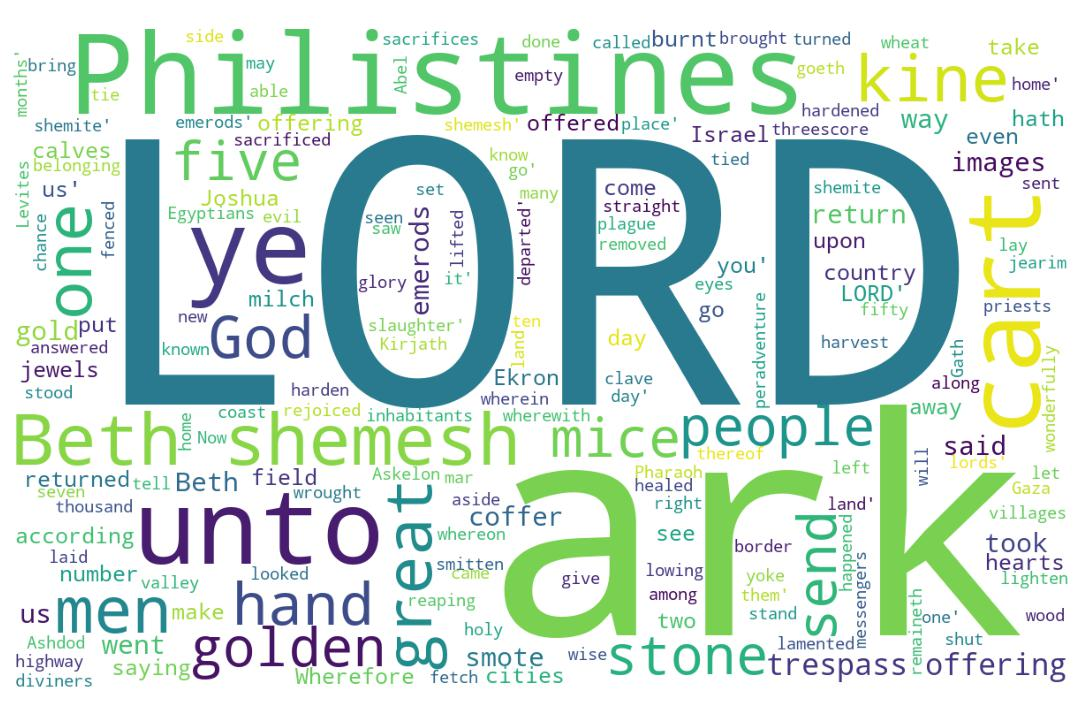
\includegraphics[width=\linewidth]{09OT-1Samuel/1Samuel6-WordCloud.jpg}
  \caption{1 Samuel 6 Word Cloud}
  \label{fig:1 Samuel 6 Word Cloud}
\end{figure}

\marginpar{\scriptsize \centering \fcolorbox{black}{lime}{\textbf{RETURNING THE ARK}}\\ (1 Samuel 6:1-21) \begin{compactenum}[I.][8]
     \item The \textbf{Cows}  \index[scripture]{1Samuel!1Sam 06:10}  (1Sa 6:10) 
    \item The \textbf{Cart} \index[scripture]{1Samuel!1Sam 06:07} \index[scripture]{1Samuel!1Sa 06:08}  \index[scripture]{1Samuel!1Sa 06:10} \index[scripture]{1Samuel!1Sa 06:11} \index[scripture]{1Samuel!1Sa 06:14}  (1Sa 6:7, 8, 10, 11, 14) 
    \item The \textbf{Coffer} \index[scripture]{1Samuel!1Sa 06:08} \index[scripture]{1Samuel!1Sa 06:11} \index[scripture]{1Samuel!1Sa 06:15}  (1Sa 6:8, 11, 15) 
    \item No \textbf{Covering}  %\index[scripture]{1Samuel!1Sam 06:10}  (1 Samuel 6:10) 
    \item The \textbf{Cities}   \index[scripture]{1Samuel!1Sa 06:17}  (1Sa 6:17) 
    \item The \textbf{Crime}   \index[scripture]{1Samuel!1Sa 06:19}  (1Sa 6:19) 
    \item The \textbf{Call}   \index[scripture]{1Samuel!1Sa 06:21}  (1Sa 6:21) 
\end{compactenum}}




\footnote{\textcolor[cmyk]{0.99998,1,0,0}{\hyperlink{TOC}{Return to end of Table of Contents.}}}\footnote{\href{https://audiobible.com/bible/1_samuel_6.html}{\textcolor[cmyk]{0.99998,1,0,0}{1 Samuel 6 Audio}}}\textcolor[cmyk]{0.99998,1,0,0}{And the ark of the LORD was in the country of the Philistines seven months.}
[2] \textcolor[cmyk]{0.99998,1,0,0}{And the Philistines called for the priests and the diviners, saying, What shall we do to the ark of the LORD? tell us wherewith we shall send it to his place.}
[3] \textcolor[cmyk]{0.99998,1,0,0}{And they said, If ye send away the ark of the God of Israel, send it not empty; but in any wise return him a trespass offering: then ye shall be healed, and it shall be known to you why his hand is not removed from you.}
[4] \textcolor[cmyk]{0.99998,1,0,0}{Then said they, What \emph{shall} \emph{be} the trespass offering which we shall return to him? They answered, Five golden emerods, and five golden mice, \emph{according} \emph{to} the number of the lords of the Philistines: for one plague \emph{was} on you all, and on your lords.}
[5] \textcolor[cmyk]{0.99998,1,0,0}{Wherefore ye shall make images of your emerods, and images of your mice that mar the land; and ye shall give glory unto the God of Israel: peradventure he will lighten his hand from off you, and from off your gods, and from off your land.}
[6] \textcolor[cmyk]{0.99998,1,0,0}{Wherefore then do ye harden your hearts, as the Egyptians and Pharaoh hardened their hearts? when he had wrought wonderfully among them, did they not let the people go, and they departed?}
[7] \textcolor[cmyk]{0.99998,1,0,0}{Now therefore make a new \fcolorbox{black}{lime}{cart}, and take two milch kine, on which there hath come no yoke, and tie the kine to the \fcolorbox{black}{lime}{cart}, and bring their calves home from them:}
[8] \textcolor[cmyk]{0.99998,1,0,0}{And take the ark of the LORD, and lay it upon the \fcolorbox{black}{lime}{cart}; and put the jewels of gold, which ye return him \emph{for} a trespass offering, in a coffer by the side thereof; and send it away, that it may go.}
[9] \textcolor[cmyk]{0.99998,1,0,0}{And see, if it goeth up by the way of his own coast to Beth-shemesh, \emph{then} he hath done us this great evil: but if not, then we shall know that \emph{it} \emph{is} not his hand \emph{that} smote us: it \emph{was} a chance \emph{that} happened to us.}\\
\\
\P \textcolor[cmyk]{0.99998,1,0,0}{And the men did so; and took two milch \fcolorbox{black}{lime}{kine}, and tied them to the \fcolorbox{black}{lime}{cart}, and shut up their calves at home:}
[11] \textcolor[cmyk]{0.99998,1,0,0}{And they laid the ark of the LORD upon the \fcolorbox{black}{lime}{cart}, and the coffer with the mice of gold and the images of their emerods.}
[12] \textcolor[cmyk]{0.99998,1,0,0}{And the kine took the straight way to the way of Beth-shemesh, \emph{and} went along the highway, lowing as they went, and turned not aside \emph{to} the right hand or \emph{to} the left; and the lords of the Philistines went after them unto the border of Beth-shemesh.}
[13] \textcolor[cmyk]{0.99998,1,0,0}{And \emph{they} \emph{of} Beth-shemesh \emph{were} reaping their wheat harvest in the valley: and they lifted up their eyes, and saw the ark, and rejoiced to see \emph{it}.}
[14] \textcolor[cmyk]{0.99998,1,0,0}{And the \fcolorbox{black}{lime}{cart} came into the field of Joshua, a Beth-shemite, and stood there, where \emph{there} \emph{was} a great stone: and they clave the wood of the \fcolorbox{black}{lime}{cart}, and offered the kine a burnt offering unto the LORD.}
[15] \textcolor[cmyk]{0.99998,1,0,0}{And the Levites took down the ark of the LORD, and the coffer that \emph{was} with it, wherein the jewels of gold \emph{were}, and put \emph{them} on the great stone: and the men of Beth-shemesh offered burnt offerings and sacrificed sacrifices the same day unto the LORD.}
[16] \textcolor[cmyk]{0.99998,1,0,0}{And when the five lords of the Philistines had seen \emph{it}, they returned to Ekron the same day.}
[17] \textcolor[cmyk]{0.99998,1,0,0}{And these \emph{are} the golden emerods which the Philistines returned \emph{for} a trespass offering unto the LORD; for \fcolorbox{black}{lime}{Ashdod} one, for \fcolorbox{black}{lime}{Gaza} one, for \fcolorbox{black}{lime}{Askelon} one, for \fcolorbox{black}{lime}{Gath} one, for \fcolorbox{black}{lime}{Ekron} one;}
[18] \textcolor[cmyk]{0.99998,1,0,0}{And the golden mice, \emph{according} \emph{to} the number of all the cities of the Philistines \emph{belonging} to the five lords, \emph{both} of fenced cities, and of country villages, even unto the great \emph{stone} \emph{of} Abel, whereon they set down the ark of the LORD: \emph{which} \emph{stone} \emph{remaineth} unto this day in the field of Joshua, the Beth-shemite.}\\
\\
\P \textcolor[cmyk]{0.99998,1,0,0}{And he smote the men of Beth-shemesh, because they had \fcolorbox{black}{lime}{looked into} the ark of the LORD, even he smote of the people fifty thousand and threescore and ten men: and the people lamented, because the LORD had smitten \emph{many} of the people with a great slaughter.}
[20] \textcolor[cmyk]{0.99998,1,0,0}{And the men of Beth-shemesh said, Who is able to stand before this holy LORD God? and to whom shall he go up from us?}\\
\\
\P \textcolor[cmyk]{0.99998,1,0,0}{And they sent messengers to the inhabitants of Kirjath-jearim, saying, The Philistines have brought again the ark of the LORD; come ye down, \emph{and} fetch it up to you.}
\section{1 Samuel 6 Comments}

\subsection{Numeric Nuggets}
\textbf{13: } The word ``LORD'' is used 13 times in the chapter.
%\index[NWIV]{15!1Samuel!1Sa 6:1}\index[AWIP]{And!1Samuel!1Sa 6:1}\index[AWIP]{the!1Samuel!1Sa 6:1}\index[AWIP]{the!1Samuel!1Sa 6:1 (2)}\index[AWIP]{the!1Samuel!1Sa 6:1 (3)}\index[AWIP]{the!1Samuel!1Sa 6:1 (4)}\index[AWIP]{ark!1Samuel!1Sa 6:1}\index[AWIP]{of!1Samuel!1Sa 6:1}\index[AWIP]{of!1Samuel!1Sa 6:1 (2)}\index[AWIP]{LORD!1Samuel!1Sa 6:1}\index[AWIP]{was!1Samuel!1Sa 6:1}\index[AWIP]{in!1Samuel!1Sa 6:1}\index[AWIP]{country!1Samuel!1Sa 6:1}\index[AWIP]{Philistines!1Samuel!1Sa 6:1}\index[AWIP]{seven!1Samuel!1Sa 6:1}\index[AWIP]{months!1Samuel!1Sa 6:1}

\index[NWIV]{31!1Samuel!1Sa 6:2}\index[AWIP]{And!1Samuel!1Sa 6:2}\index[AWIP]{the!1Samuel!1Sa 6:2}\index[AWIP]{the!1Samuel!1Sa 6:2 (2)}\index[AWIP]{the!1Samuel!1Sa 6:2 (3)}\index[AWIP]{the!1Samuel!1Sa 6:2 (4)}\index[AWIP]{the!1Samuel!1Sa 6:2 (5)}\index[AWIP]{Philistines!1Samuel!1Sa 6:2}\index[AWIP]{called!1Samuel!1Sa 6:2}\index[AWIP]{for!1Samuel!1Sa 6:2}\index[AWIP]{priests!1Samuel!1Sa 6:2}\index[AWIP]{and!1Samuel!1Sa 6:2}\index[AWIP]{diviners!1Samuel!1Sa 6:2}\index[AWIP]{saying!1Samuel!1Sa 6:2}\index[AWIP]{What!1Samuel!1Sa 6:2}\index[AWIP]{shall!1Samuel!1Sa 6:2}\index[AWIP]{shall!1Samuel!1Sa 6:2 (2)}\index[AWIP]{we!1Samuel!1Sa 6:2}\index[AWIP]{we!1Samuel!1Sa 6:2 (2)}\index[AWIP]{do!1Samuel!1Sa 6:2}\index[AWIP]{to!1Samuel!1Sa 6:2}\index[AWIP]{to!1Samuel!1Sa 6:2 (2)}\index[AWIP]{ark!1Samuel!1Sa 6:2}\index[AWIP]{of!1Samuel!1Sa 6:2}\index[AWIP]{LORD?!1Samuel!1Sa 6:2}\index[AWIP]{tell!1Samuel!1Sa 6:2}\index[AWIP]{us!1Samuel!1Sa 6:2}\index[AWIP]{wherewith!1Samuel!1Sa 6:2}\index[AWIP]{send!1Samuel!1Sa 6:2}\index[AWIP]{it!1Samuel!1Sa 6:2}\index[AWIP]{his!1Samuel!1Sa 6:2}\index[AWIP]{place!1Samuel!1Sa 6:2}

\index[NWIV]{47!1Samuel!1Sa 6:3}\index[AWIP]{And!1Samuel!1Sa 6:3}\index[AWIP]{they!1Samuel!1Sa 6:3}\index[AWIP]{said!1Samuel!1Sa 6:3}\index[AWIP]{If!1Samuel!1Sa 6:3}\index[AWIP]{ye!1Samuel!1Sa 6:3}\index[AWIP]{ye!1Samuel!1Sa 6:3 (2)}\index[AWIP]{send!1Samuel!1Sa 6:3}\index[AWIP]{send!1Samuel!1Sa 6:3 (2)}\index[AWIP]{away!1Samuel!1Sa 6:3}\index[AWIP]{the!1Samuel!1Sa 6:3}\index[AWIP]{the!1Samuel!1Sa 6:3 (2)}\index[AWIP]{ark!1Samuel!1Sa 6:3}\index[AWIP]{of!1Samuel!1Sa 6:3}\index[AWIP]{of!1Samuel!1Sa 6:3 (2)}\index[AWIP]{God!1Samuel!1Sa 6:3}\index[AWIP]{Israel!1Samuel!1Sa 6:3}\index[AWIP]{it!1Samuel!1Sa 6:3}\index[AWIP]{it!1Samuel!1Sa 6:3 (2)}\index[AWIP]{not!1Samuel!1Sa 6:3}\index[AWIP]{not!1Samuel!1Sa 6:3 (2)}\index[AWIP]{empty!1Samuel!1Sa 6:3}\index[AWIP]{but!1Samuel!1Sa 6:3}\index[AWIP]{in!1Samuel!1Sa 6:3}\index[AWIP]{any!1Samuel!1Sa 6:3}\index[AWIP]{wise!1Samuel!1Sa 6:3}\index[AWIP]{return!1Samuel!1Sa 6:3}\index[AWIP]{him!1Samuel!1Sa 6:3}\index[AWIP]{a!1Samuel!1Sa 6:3}\index[AWIP]{trespass!1Samuel!1Sa 6:3}\index[AWIP]{offering!1Samuel!1Sa 6:3}\index[AWIP]{then!1Samuel!1Sa 6:3}\index[AWIP]{shall!1Samuel!1Sa 6:3}\index[AWIP]{shall!1Samuel!1Sa 6:3 (2)}\index[AWIP]{be!1Samuel!1Sa 6:3}\index[AWIP]{be!1Samuel!1Sa 6:3 (2)}\index[AWIP]{healed!1Samuel!1Sa 6:3}\index[AWIP]{and!1Samuel!1Sa 6:3}\index[AWIP]{known!1Samuel!1Sa 6:3}\index[AWIP]{to!1Samuel!1Sa 6:3}\index[AWIP]{you!1Samuel!1Sa 6:3}\index[AWIP]{you!1Samuel!1Sa 6:3 (2)}\index[AWIP]{why!1Samuel!1Sa 6:3}\index[AWIP]{his!1Samuel!1Sa 6:3}\index[AWIP]{hand!1Samuel!1Sa 6:3}\index[AWIP]{is!1Samuel!1Sa 6:3}\index[AWIP]{removed!1Samuel!1Sa 6:3}\index[AWIP]{from!1Samuel!1Sa 6:3}

\index[NWIV]{45!1Samuel!1Sa 6:4}\index[AWIP]{Then!1Samuel!1Sa 6:4}\index[AWIP]{said!1Samuel!1Sa 6:4}\index[AWIP]{they!1Samuel!1Sa 6:4}\index[AWIP]{What!1Samuel!1Sa 6:4}\index[AWIP]{\emph{shall}!1Samuel!1Sa 6:4}\index[AWIP]{\emph{be}!1Samuel!1Sa 6:4}\index[AWIP]{the!1Samuel!1Sa 6:4}\index[AWIP]{the!1Samuel!1Sa 6:4 (2)}\index[AWIP]{the!1Samuel!1Sa 6:4 (3)}\index[AWIP]{the!1Samuel!1Sa 6:4 (4)}\index[AWIP]{trespass!1Samuel!1Sa 6:4}\index[AWIP]{offering!1Samuel!1Sa 6:4}\index[AWIP]{which!1Samuel!1Sa 6:4}\index[AWIP]{we!1Samuel!1Sa 6:4}\index[AWIP]{shall!1Samuel!1Sa 6:4}\index[AWIP]{return!1Samuel!1Sa 6:4}\index[AWIP]{to!1Samuel!1Sa 6:4}\index[AWIP]{him?!1Samuel!1Sa 6:4}\index[AWIP]{They!1Samuel!1Sa 6:4}\index[AWIP]{answered!1Samuel!1Sa 6:4}\index[AWIP]{Five!1Samuel!1Sa 6:4}\index[AWIP]{golden!1Samuel!1Sa 6:4}\index[AWIP]{golden!1Samuel!1Sa 6:4 (2)}\index[AWIP]{emerods!1Samuel!1Sa 6:4}\index[AWIP]{and!1Samuel!1Sa 6:4}\index[AWIP]{and!1Samuel!1Sa 6:4 (2)}\index[AWIP]{five!1Samuel!1Sa 6:4}\index[AWIP]{mice!1Samuel!1Sa 6:4}\index[AWIP]{\emph{according}!1Samuel!1Sa 6:4}\index[AWIP]{\emph{to}!1Samuel!1Sa 6:4}\index[AWIP]{number!1Samuel!1Sa 6:4}\index[AWIP]{of!1Samuel!1Sa 6:4}\index[AWIP]{of!1Samuel!1Sa 6:4 (2)}\index[AWIP]{lords!1Samuel!1Sa 6:4}\index[AWIP]{lords!1Samuel!1Sa 6:4 (2)}\index[AWIP]{Philistines!1Samuel!1Sa 6:4}\index[AWIP]{for!1Samuel!1Sa 6:4}\index[AWIP]{one!1Samuel!1Sa 6:4}\index[AWIP]{plague!1Samuel!1Sa 6:4}\index[AWIP]{\emph{was}!1Samuel!1Sa 6:4}\index[AWIP]{on!1Samuel!1Sa 6:4}\index[AWIP]{on!1Samuel!1Sa 6:4 (2)}\index[AWIP]{you!1Samuel!1Sa 6:4}\index[AWIP]{all!1Samuel!1Sa 6:4}\index[AWIP]{your!1Samuel!1Sa 6:4}\index[AWIP]{\emph{shall}!1Samuel!1Sa 6:4}\index[AWIP]{\emph{be}!1Samuel!1Sa 6:4}\index[AWIP]{\emph{according}!1Samuel!1Sa 6:4}\index[AWIP]{\emph{to}!1Samuel!1Sa 6:4}\index[AWIP]{\emph{was}!1Samuel!1Sa 6:4}

\index[NWIV]{46!1Samuel!1Sa 6:5}\index[AWIP]{Wherefore!1Samuel!1Sa 6:5}\index[AWIP]{ye!1Samuel!1Sa 6:5}\index[AWIP]{ye!1Samuel!1Sa 6:5 (2)}\index[AWIP]{shall!1Samuel!1Sa 6:5}\index[AWIP]{shall!1Samuel!1Sa 6:5 (2)}\index[AWIP]{make!1Samuel!1Sa 6:5}\index[AWIP]{images!1Samuel!1Sa 6:5}\index[AWIP]{images!1Samuel!1Sa 6:5 (2)}\index[AWIP]{of!1Samuel!1Sa 6:5}\index[AWIP]{of!1Samuel!1Sa 6:5 (2)}\index[AWIP]{of!1Samuel!1Sa 6:5 (3)}\index[AWIP]{your!1Samuel!1Sa 6:5}\index[AWIP]{your!1Samuel!1Sa 6:5 (2)}\index[AWIP]{your!1Samuel!1Sa 6:5 (3)}\index[AWIP]{your!1Samuel!1Sa 6:5 (4)}\index[AWIP]{emerods!1Samuel!1Sa 6:5}\index[AWIP]{and!1Samuel!1Sa 6:5}\index[AWIP]{and!1Samuel!1Sa 6:5 (2)}\index[AWIP]{and!1Samuel!1Sa 6:5 (3)}\index[AWIP]{and!1Samuel!1Sa 6:5 (4)}\index[AWIP]{mice!1Samuel!1Sa 6:5}\index[AWIP]{that!1Samuel!1Sa 6:5}\index[AWIP]{mar!1Samuel!1Sa 6:5}\index[AWIP]{the!1Samuel!1Sa 6:5}\index[AWIP]{the!1Samuel!1Sa 6:5 (2)}\index[AWIP]{land!1Samuel!1Sa 6:5}\index[AWIP]{land!1Samuel!1Sa 6:5 (2)}\index[AWIP]{give!1Samuel!1Sa 6:5}\index[AWIP]{glory!1Samuel!1Sa 6:5}\index[AWIP]{unto!1Samuel!1Sa 6:5}\index[AWIP]{God!1Samuel!1Sa 6:5}\index[AWIP]{Israel!1Samuel!1Sa 6:5}\index[AWIP]{peradventure!1Samuel!1Sa 6:5}\index[AWIP]{he!1Samuel!1Sa 6:5}\index[AWIP]{will!1Samuel!1Sa 6:5}\index[AWIP]{lighten!1Samuel!1Sa 6:5}\index[AWIP]{his!1Samuel!1Sa 6:5}\index[AWIP]{hand!1Samuel!1Sa 6:5}\index[AWIP]{from!1Samuel!1Sa 6:5}\index[AWIP]{from!1Samuel!1Sa 6:5 (2)}\index[AWIP]{from!1Samuel!1Sa 6:5 (3)}\index[AWIP]{off!1Samuel!1Sa 6:5}\index[AWIP]{off!1Samuel!1Sa 6:5 (2)}\index[AWIP]{off!1Samuel!1Sa 6:5 (3)}\index[AWIP]{you!1Samuel!1Sa 6:5}\index[AWIP]{gods!1Samuel!1Sa 6:5}

\index[NWIV]{32!1Samuel!1Sa 6:6}\index[AWIP]{Wherefore!1Samuel!1Sa 6:6}\index[AWIP]{then!1Samuel!1Sa 6:6}\index[AWIP]{do!1Samuel!1Sa 6:6}\index[AWIP]{ye!1Samuel!1Sa 6:6}\index[AWIP]{harden!1Samuel!1Sa 6:6}\index[AWIP]{your!1Samuel!1Sa 6:6}\index[AWIP]{hearts!1Samuel!1Sa 6:6}\index[AWIP]{as!1Samuel!1Sa 6:6}\index[AWIP]{the!1Samuel!1Sa 6:6}\index[AWIP]{the!1Samuel!1Sa 6:6 (2)}\index[AWIP]{Egyptians!1Samuel!1Sa 6:6}\index[AWIP]{and!1Samuel!1Sa 6:6}\index[AWIP]{and!1Samuel!1Sa 6:6 (2)}\index[AWIP]{Pharaoh!1Samuel!1Sa 6:6}\index[AWIP]{hardened!1Samuel!1Sa 6:6}\index[AWIP]{their!1Samuel!1Sa 6:6}\index[AWIP]{hearts?!1Samuel!1Sa 6:6}\index[AWIP]{when!1Samuel!1Sa 6:6}\index[AWIP]{he!1Samuel!1Sa 6:6}\index[AWIP]{had!1Samuel!1Sa 6:6}\index[AWIP]{wrought!1Samuel!1Sa 6:6}\index[AWIP]{wonderfully!1Samuel!1Sa 6:6}\index[AWIP]{among!1Samuel!1Sa 6:6}\index[AWIP]{them!1Samuel!1Sa 6:6}\index[AWIP]{did!1Samuel!1Sa 6:6}\index[AWIP]{they!1Samuel!1Sa 6:6}\index[AWIP]{they!1Samuel!1Sa 6:6 (2)}\index[AWIP]{not!1Samuel!1Sa 6:6}\index[AWIP]{let!1Samuel!1Sa 6:6}\index[AWIP]{people!1Samuel!1Sa 6:6}\index[AWIP]{go!1Samuel!1Sa 6:6}\index[AWIP]{departed?!1Samuel!1Sa 6:6}

\index[NWIV]{32!1Samuel!1Sa 6:7}\index[AWIP]{Now!1Samuel!1Sa 6:7}\index[AWIP]{therefore!1Samuel!1Sa 6:7}\index[AWIP]{make!1Samuel!1Sa 6:7}\index[AWIP]{a!1Samuel!1Sa 6:7}\index[AWIP]{new!1Samuel!1Sa 6:7}\index[AWIP]{cart!1Samuel!1Sa 6:7}\index[AWIP]{cart!1Samuel!1Sa 6:7 (2)}\index[AWIP]{and!1Samuel!1Sa 6:7}\index[AWIP]{and!1Samuel!1Sa 6:7 (2)}\index[AWIP]{and!1Samuel!1Sa 6:7 (3)}\index[AWIP]{take!1Samuel!1Sa 6:7}\index[AWIP]{two!1Samuel!1Sa 6:7}\index[AWIP]{milch!1Samuel!1Sa 6:7}\index[AWIP]{kine!1Samuel!1Sa 6:7}\index[AWIP]{kine!1Samuel!1Sa 6:7 (2)}\index[AWIP]{on!1Samuel!1Sa 6:7}\index[AWIP]{which!1Samuel!1Sa 6:7}\index[AWIP]{there!1Samuel!1Sa 6:7}\index[AWIP]{hath!1Samuel!1Sa 6:7}\index[AWIP]{come!1Samuel!1Sa 6:7}\index[AWIP]{no!1Samuel!1Sa 6:7}\index[AWIP]{yoke!1Samuel!1Sa 6:7}\index[AWIP]{tie!1Samuel!1Sa 6:7}\index[AWIP]{the!1Samuel!1Sa 6:7}\index[AWIP]{the!1Samuel!1Sa 6:7 (2)}\index[AWIP]{to!1Samuel!1Sa 6:7}\index[AWIP]{bring!1Samuel!1Sa 6:7}\index[AWIP]{their!1Samuel!1Sa 6:7}\index[AWIP]{calves!1Samuel!1Sa 6:7}\index[AWIP]{home!1Samuel!1Sa 6:7}\index[AWIP]{from!1Samuel!1Sa 6:7}\index[AWIP]{them!1Samuel!1Sa 6:7}

\index[NWIV]{42!1Samuel!1Sa 6:8}\index[AWIP]{And!1Samuel!1Sa 6:8}\index[AWIP]{take!1Samuel!1Sa 6:8}\index[AWIP]{the!1Samuel!1Sa 6:8}\index[AWIP]{the!1Samuel!1Sa 6:8 (2)}\index[AWIP]{the!1Samuel!1Sa 6:8 (3)}\index[AWIP]{the!1Samuel!1Sa 6:8 (4)}\index[AWIP]{the!1Samuel!1Sa 6:8 (5)}\index[AWIP]{ark!1Samuel!1Sa 6:8}\index[AWIP]{of!1Samuel!1Sa 6:8}\index[AWIP]{of!1Samuel!1Sa 6:8 (2)}\index[AWIP]{LORD!1Samuel!1Sa 6:8}\index[AWIP]{and!1Samuel!1Sa 6:8}\index[AWIP]{and!1Samuel!1Sa 6:8 (2)}\index[AWIP]{and!1Samuel!1Sa 6:8 (3)}\index[AWIP]{lay!1Samuel!1Sa 6:8}\index[AWIP]{it!1Samuel!1Sa 6:8}\index[AWIP]{it!1Samuel!1Sa 6:8 (2)}\index[AWIP]{it!1Samuel!1Sa 6:8 (3)}\index[AWIP]{upon!1Samuel!1Sa 6:8}\index[AWIP]{cart!1Samuel!1Sa 6:8}\index[AWIP]{put!1Samuel!1Sa 6:8}\index[AWIP]{jewels!1Samuel!1Sa 6:8}\index[AWIP]{gold!1Samuel!1Sa 6:8}\index[AWIP]{which!1Samuel!1Sa 6:8}\index[AWIP]{ye!1Samuel!1Sa 6:8}\index[AWIP]{return!1Samuel!1Sa 6:8}\index[AWIP]{him!1Samuel!1Sa 6:8}\index[AWIP]{\emph{for}!1Samuel!1Sa 6:8}\index[AWIP]{a!1Samuel!1Sa 6:8}\index[AWIP]{a!1Samuel!1Sa 6:8 (2)}\index[AWIP]{trespass!1Samuel!1Sa 6:8}\index[AWIP]{offering!1Samuel!1Sa 6:8}\index[AWIP]{in!1Samuel!1Sa 6:8}\index[AWIP]{coffer!1Samuel!1Sa 6:8}\index[AWIP]{by!1Samuel!1Sa 6:8}\index[AWIP]{side!1Samuel!1Sa 6:8}\index[AWIP]{thereof!1Samuel!1Sa 6:8}\index[AWIP]{send!1Samuel!1Sa 6:8}\index[AWIP]{away!1Samuel!1Sa 6:8}\index[AWIP]{that!1Samuel!1Sa 6:8}\index[AWIP]{may!1Samuel!1Sa 6:8}\index[AWIP]{go!1Samuel!1Sa 6:8}\index[AWIP]{\emph{for}!1Samuel!1Sa 6:8}

\index[NWIV]{47!1Samuel!1Sa 6:9}\index[AWIP]{And!1Samuel!1Sa 6:9}\index[AWIP]{see!1Samuel!1Sa 6:9}\index[AWIP]{if!1Samuel!1Sa 6:9}\index[AWIP]{if!1Samuel!1Sa 6:9 (2)}\index[AWIP]{it!1Samuel!1Sa 6:9}\index[AWIP]{it!1Samuel!1Sa 6:9 (2)}\index[AWIP]{goeth!1Samuel!1Sa 6:9}\index[AWIP]{up!1Samuel!1Sa 6:9}\index[AWIP]{by!1Samuel!1Sa 6:9}\index[AWIP]{the!1Samuel!1Sa 6:9}\index[AWIP]{way!1Samuel!1Sa 6:9}\index[AWIP]{of!1Samuel!1Sa 6:9}\index[AWIP]{his!1Samuel!1Sa 6:9}\index[AWIP]{his!1Samuel!1Sa 6:9 (2)}\index[AWIP]{own!1Samuel!1Sa 6:9}\index[AWIP]{coast!1Samuel!1Sa 6:9}\index[AWIP]{to!1Samuel!1Sa 6:9}\index[AWIP]{to!1Samuel!1Sa 6:9 (2)}\index[AWIP]{Beth-shemesh!1Samuel!1Sa 6:9}\index[AWIP]{\emph{then}!1Samuel!1Sa 6:9}\index[AWIP]{he!1Samuel!1Sa 6:9}\index[AWIP]{hath!1Samuel!1Sa 6:9}\index[AWIP]{done!1Samuel!1Sa 6:9}\index[AWIP]{us!1Samuel!1Sa 6:9}\index[AWIP]{us!1Samuel!1Sa 6:9 (2)}\index[AWIP]{us!1Samuel!1Sa 6:9 (3)}\index[AWIP]{this!1Samuel!1Sa 6:9}\index[AWIP]{great!1Samuel!1Sa 6:9}\index[AWIP]{evil!1Samuel!1Sa 6:9}\index[AWIP]{but!1Samuel!1Sa 6:9}\index[AWIP]{not!1Samuel!1Sa 6:9}\index[AWIP]{not!1Samuel!1Sa 6:9 (2)}\index[AWIP]{then!1Samuel!1Sa 6:9}\index[AWIP]{we!1Samuel!1Sa 6:9}\index[AWIP]{shall!1Samuel!1Sa 6:9}\index[AWIP]{know!1Samuel!1Sa 6:9}\index[AWIP]{that!1Samuel!1Sa 6:9}\index[AWIP]{\emph{it}!1Samuel!1Sa 6:9}\index[AWIP]{\emph{is}!1Samuel!1Sa 6:9}\index[AWIP]{hand!1Samuel!1Sa 6:9}\index[AWIP]{\emph{that}!1Samuel!1Sa 6:9}\index[AWIP]{\emph{that}!1Samuel!1Sa 6:9 (2)}\index[AWIP]{smote!1Samuel!1Sa 6:9}\index[AWIP]{\emph{was}!1Samuel!1Sa 6:9}\index[AWIP]{a!1Samuel!1Sa 6:9}\index[AWIP]{chance!1Samuel!1Sa 6:9}\index[AWIP]{happened!1Samuel!1Sa 6:9}\index[AWIP]{\emph{then}!1Samuel!1Sa 6:9}\index[AWIP]{\emph{it}!1Samuel!1Sa 6:9}\index[AWIP]{\emph{is}!1Samuel!1Sa 6:9}\index[AWIP]{\emph{that}!1Samuel!1Sa 6:9}\index[AWIP]{\emph{that}!1Samuel!1Sa 6:9 (2)}\index[AWIP]{\emph{was}!1Samuel!1Sa 6:9}

\index[NWIV]{23!1Samuel!1Sa 6:10}\index[AWIP]{And!1Samuel!1Sa 6:10}\index[AWIP]{the!1Samuel!1Sa 6:10}\index[AWIP]{the!1Samuel!1Sa 6:10 (2)}\index[AWIP]{men!1Samuel!1Sa 6:10}\index[AWIP]{did!1Samuel!1Sa 6:10}\index[AWIP]{so!1Samuel!1Sa 6:10}\index[AWIP]{and!1Samuel!1Sa 6:10}\index[AWIP]{and!1Samuel!1Sa 6:10 (2)}\index[AWIP]{and!1Samuel!1Sa 6:10 (3)}\index[AWIP]{took!1Samuel!1Sa 6:10}\index[AWIP]{two!1Samuel!1Sa 6:10}\index[AWIP]{milch!1Samuel!1Sa 6:10}\index[AWIP]{kine!1Samuel!1Sa 6:10}\index[AWIP]{tied!1Samuel!1Sa 6:10}\index[AWIP]{them!1Samuel!1Sa 6:10}\index[AWIP]{to!1Samuel!1Sa 6:10}\index[AWIP]{cart!1Samuel!1Sa 6:10}\index[AWIP]{shut!1Samuel!1Sa 6:10}\index[AWIP]{up!1Samuel!1Sa 6:10}\index[AWIP]{their!1Samuel!1Sa 6:10}\index[AWIP]{calves!1Samuel!1Sa 6:10}\index[AWIP]{at!1Samuel!1Sa 6:10}\index[AWIP]{home!1Samuel!1Sa 6:10}

\index[NWIV]{25!1Samuel!1Sa 6:11}\index[AWIP]{And!1Samuel!1Sa 6:11}\index[AWIP]{they!1Samuel!1Sa 6:11}\index[AWIP]{laid!1Samuel!1Sa 6:11}\index[AWIP]{the!1Samuel!1Sa 6:11}\index[AWIP]{the!1Samuel!1Sa 6:11 (2)}\index[AWIP]{the!1Samuel!1Sa 6:11 (3)}\index[AWIP]{the!1Samuel!1Sa 6:11 (4)}\index[AWIP]{the!1Samuel!1Sa 6:11 (5)}\index[AWIP]{the!1Samuel!1Sa 6:11 (6)}\index[AWIP]{ark!1Samuel!1Sa 6:11}\index[AWIP]{of!1Samuel!1Sa 6:11}\index[AWIP]{of!1Samuel!1Sa 6:11 (2)}\index[AWIP]{of!1Samuel!1Sa 6:11 (3)}\index[AWIP]{LORD!1Samuel!1Sa 6:11}\index[AWIP]{upon!1Samuel!1Sa 6:11}\index[AWIP]{cart!1Samuel!1Sa 6:11}\index[AWIP]{and!1Samuel!1Sa 6:11}\index[AWIP]{and!1Samuel!1Sa 6:11 (2)}\index[AWIP]{coffer!1Samuel!1Sa 6:11}\index[AWIP]{with!1Samuel!1Sa 6:11}\index[AWIP]{mice!1Samuel!1Sa 6:11}\index[AWIP]{gold!1Samuel!1Sa 6:11}\index[AWIP]{images!1Samuel!1Sa 6:11}\index[AWIP]{their!1Samuel!1Sa 6:11}\index[AWIP]{emerods!1Samuel!1Sa 6:11}

\index[NWIV]{47!1Samuel!1Sa 6:12}\index[AWIP]{And!1Samuel!1Sa 6:12}\index[AWIP]{the!1Samuel!1Sa 6:12}\index[AWIP]{the!1Samuel!1Sa 6:12 (2)}\index[AWIP]{the!1Samuel!1Sa 6:12 (3)}\index[AWIP]{the!1Samuel!1Sa 6:12 (4)}\index[AWIP]{the!1Samuel!1Sa 6:12 (5)}\index[AWIP]{the!1Samuel!1Sa 6:12 (6)}\index[AWIP]{the!1Samuel!1Sa 6:12 (7)}\index[AWIP]{the!1Samuel!1Sa 6:12 (8)}\index[AWIP]{the!1Samuel!1Sa 6:12 (9)}\index[AWIP]{kine!1Samuel!1Sa 6:12}\index[AWIP]{took!1Samuel!1Sa 6:12}\index[AWIP]{straight!1Samuel!1Sa 6:12}\index[AWIP]{way!1Samuel!1Sa 6:12}\index[AWIP]{way!1Samuel!1Sa 6:12 (2)}\index[AWIP]{to!1Samuel!1Sa 6:12}\index[AWIP]{of!1Samuel!1Sa 6:12}\index[AWIP]{of!1Samuel!1Sa 6:12 (2)}\index[AWIP]{of!1Samuel!1Sa 6:12 (3)}\index[AWIP]{Beth-shemesh!1Samuel!1Sa 6:12}\index[AWIP]{Beth-shemesh!1Samuel!1Sa 6:12 (2)}\index[AWIP]{\emph{and}!1Samuel!1Sa 6:12}\index[AWIP]{went!1Samuel!1Sa 6:12}\index[AWIP]{went!1Samuel!1Sa 6:12 (2)}\index[AWIP]{went!1Samuel!1Sa 6:12 (3)}\index[AWIP]{along!1Samuel!1Sa 6:12}\index[AWIP]{highway!1Samuel!1Sa 6:12}\index[AWIP]{lowing!1Samuel!1Sa 6:12}\index[AWIP]{as!1Samuel!1Sa 6:12}\index[AWIP]{they!1Samuel!1Sa 6:12}\index[AWIP]{and!1Samuel!1Sa 6:12}\index[AWIP]{and!1Samuel!1Sa 6:12 (2)}\index[AWIP]{turned!1Samuel!1Sa 6:12}\index[AWIP]{not!1Samuel!1Sa 6:12}\index[AWIP]{aside!1Samuel!1Sa 6:12}\index[AWIP]{\emph{to}!1Samuel!1Sa 6:12}\index[AWIP]{\emph{to}!1Samuel!1Sa 6:12 (2)}\index[AWIP]{right!1Samuel!1Sa 6:12}\index[AWIP]{hand!1Samuel!1Sa 6:12}\index[AWIP]{or!1Samuel!1Sa 6:12}\index[AWIP]{left!1Samuel!1Sa 6:12}\index[AWIP]{lords!1Samuel!1Sa 6:12}\index[AWIP]{Philistines!1Samuel!1Sa 6:12}\index[AWIP]{after!1Samuel!1Sa 6:12}\index[AWIP]{them!1Samuel!1Sa 6:12}\index[AWIP]{unto!1Samuel!1Sa 6:12}\index[AWIP]{border!1Samuel!1Sa 6:12}\index[AWIP]{\emph{and}!1Samuel!1Sa 6:12}\index[AWIP]{\emph{to}!1Samuel!1Sa 6:12}\index[AWIP]{\emph{to}!1Samuel!1Sa 6:12 (2)}

\index[NWIV]{27!1Samuel!1Sa 6:13}\index[AWIP]{And!1Samuel!1Sa 6:13}\index[AWIP]{\emph{they}!1Samuel!1Sa 6:13}\index[AWIP]{\emph{of}!1Samuel!1Sa 6:13}\index[AWIP]{Beth-shemesh!1Samuel!1Sa 6:13}\index[AWIP]{\emph{were}!1Samuel!1Sa 6:13}\index[AWIP]{reaping!1Samuel!1Sa 6:13}\index[AWIP]{their!1Samuel!1Sa 6:13}\index[AWIP]{their!1Samuel!1Sa 6:13 (2)}\index[AWIP]{wheat!1Samuel!1Sa 6:13}\index[AWIP]{harvest!1Samuel!1Sa 6:13}\index[AWIP]{in!1Samuel!1Sa 6:13}\index[AWIP]{the!1Samuel!1Sa 6:13}\index[AWIP]{the!1Samuel!1Sa 6:13 (2)}\index[AWIP]{valley!1Samuel!1Sa 6:13}\index[AWIP]{and!1Samuel!1Sa 6:13}\index[AWIP]{and!1Samuel!1Sa 6:13 (2)}\index[AWIP]{and!1Samuel!1Sa 6:13 (3)}\index[AWIP]{they!1Samuel!1Sa 6:13}\index[AWIP]{lifted!1Samuel!1Sa 6:13}\index[AWIP]{up!1Samuel!1Sa 6:13}\index[AWIP]{eyes!1Samuel!1Sa 6:13}\index[AWIP]{saw!1Samuel!1Sa 6:13}\index[AWIP]{ark!1Samuel!1Sa 6:13}\index[AWIP]{rejoiced!1Samuel!1Sa 6:13}\index[AWIP]{to!1Samuel!1Sa 6:13}\index[AWIP]{see!1Samuel!1Sa 6:13}\index[AWIP]{\emph{it}!1Samuel!1Sa 6:13}\index[AWIP]{\emph{they}!1Samuel!1Sa 6:13}\index[AWIP]{\emph{of}!1Samuel!1Sa 6:13}\index[AWIP]{\emph{were}!1Samuel!1Sa 6:13}\index[AWIP]{\emph{it}!1Samuel!1Sa 6:13}

\index[NWIV]{38!1Samuel!1Sa 6:14}\index[AWIP]{And!1Samuel!1Sa 6:14}\index[AWIP]{the!1Samuel!1Sa 6:14}\index[AWIP]{the!1Samuel!1Sa 6:14 (2)}\index[AWIP]{the!1Samuel!1Sa 6:14 (3)}\index[AWIP]{the!1Samuel!1Sa 6:14 (4)}\index[AWIP]{the!1Samuel!1Sa 6:14 (5)}\index[AWIP]{the!1Samuel!1Sa 6:14 (6)}\index[AWIP]{cart!1Samuel!1Sa 6:14}\index[AWIP]{cart!1Samuel!1Sa 6:14 (2)}\index[AWIP]{came!1Samuel!1Sa 6:14}\index[AWIP]{into!1Samuel!1Sa 6:14}\index[AWIP]{field!1Samuel!1Sa 6:14}\index[AWIP]{of!1Samuel!1Sa 6:14}\index[AWIP]{of!1Samuel!1Sa 6:14 (2)}\index[AWIP]{Joshua!1Samuel!1Sa 6:14}\index[AWIP]{a!1Samuel!1Sa 6:14}\index[AWIP]{a!1Samuel!1Sa 6:14 (2)}\index[AWIP]{a!1Samuel!1Sa 6:14 (3)}\index[AWIP]{Beth-shemite!1Samuel!1Sa 6:14}\index[AWIP]{and!1Samuel!1Sa 6:14}\index[AWIP]{and!1Samuel!1Sa 6:14 (2)}\index[AWIP]{and!1Samuel!1Sa 6:14 (3)}\index[AWIP]{stood!1Samuel!1Sa 6:14}\index[AWIP]{there!1Samuel!1Sa 6:14}\index[AWIP]{where!1Samuel!1Sa 6:14}\index[AWIP]{\emph{there}!1Samuel!1Sa 6:14}\index[AWIP]{\emph{was}!1Samuel!1Sa 6:14}\index[AWIP]{great!1Samuel!1Sa 6:14}\index[AWIP]{stone!1Samuel!1Sa 6:14}\index[AWIP]{they!1Samuel!1Sa 6:14}\index[AWIP]{clave!1Samuel!1Sa 6:14}\index[AWIP]{wood!1Samuel!1Sa 6:14}\index[AWIP]{offered!1Samuel!1Sa 6:14}\index[AWIP]{kine!1Samuel!1Sa 6:14}\index[AWIP]{burnt!1Samuel!1Sa 6:14}\index[AWIP]{offering!1Samuel!1Sa 6:14}\index[AWIP]{unto!1Samuel!1Sa 6:14}\index[AWIP]{LORD!1Samuel!1Sa 6:14}\index[AWIP]{\emph{there}!1Samuel!1Sa 6:14}\index[AWIP]{\emph{was}!1Samuel!1Sa 6:14}

\index[NWIV]{47!1Samuel!1Sa 6:15}\index[AWIP]{And!1Samuel!1Sa 6:15}\index[AWIP]{the!1Samuel!1Sa 6:15}\index[AWIP]{the!1Samuel!1Sa 6:15 (2)}\index[AWIP]{the!1Samuel!1Sa 6:15 (3)}\index[AWIP]{the!1Samuel!1Sa 6:15 (4)}\index[AWIP]{the!1Samuel!1Sa 6:15 (5)}\index[AWIP]{the!1Samuel!1Sa 6:15 (6)}\index[AWIP]{the!1Samuel!1Sa 6:15 (7)}\index[AWIP]{the!1Samuel!1Sa 6:15 (8)}\index[AWIP]{the!1Samuel!1Sa 6:15 (9)}\index[AWIP]{Levites!1Samuel!1Sa 6:15}\index[AWIP]{took!1Samuel!1Sa 6:15}\index[AWIP]{down!1Samuel!1Sa 6:15}\index[AWIP]{ark!1Samuel!1Sa 6:15}\index[AWIP]{of!1Samuel!1Sa 6:15}\index[AWIP]{of!1Samuel!1Sa 6:15 (2)}\index[AWIP]{of!1Samuel!1Sa 6:15 (3)}\index[AWIP]{LORD!1Samuel!1Sa 6:15}\index[AWIP]{LORD!1Samuel!1Sa 6:15 (2)}\index[AWIP]{and!1Samuel!1Sa 6:15}\index[AWIP]{and!1Samuel!1Sa 6:15 (2)}\index[AWIP]{and!1Samuel!1Sa 6:15 (3)}\index[AWIP]{and!1Samuel!1Sa 6:15 (4)}\index[AWIP]{coffer!1Samuel!1Sa 6:15}\index[AWIP]{that!1Samuel!1Sa 6:15}\index[AWIP]{\emph{was}!1Samuel!1Sa 6:15}\index[AWIP]{with!1Samuel!1Sa 6:15}\index[AWIP]{it!1Samuel!1Sa 6:15}\index[AWIP]{wherein!1Samuel!1Sa 6:15}\index[AWIP]{jewels!1Samuel!1Sa 6:15}\index[AWIP]{gold!1Samuel!1Sa 6:15}\index[AWIP]{\emph{were}!1Samuel!1Sa 6:15}\index[AWIP]{put!1Samuel!1Sa 6:15}\index[AWIP]{\emph{them}!1Samuel!1Sa 6:15}\index[AWIP]{on!1Samuel!1Sa 6:15}\index[AWIP]{great!1Samuel!1Sa 6:15}\index[AWIP]{stone!1Samuel!1Sa 6:15}\index[AWIP]{men!1Samuel!1Sa 6:15}\index[AWIP]{Beth-shemesh!1Samuel!1Sa 6:15}\index[AWIP]{offered!1Samuel!1Sa 6:15}\index[AWIP]{burnt!1Samuel!1Sa 6:15}\index[AWIP]{offerings!1Samuel!1Sa 6:15}\index[AWIP]{sacrificed!1Samuel!1Sa 6:15}\index[AWIP]{sacrifices!1Samuel!1Sa 6:15}\index[AWIP]{same!1Samuel!1Sa 6:15}\index[AWIP]{day!1Samuel!1Sa 6:15}\index[AWIP]{unto!1Samuel!1Sa 6:15}\index[AWIP]{\emph{was}!1Samuel!1Sa 6:15}\index[AWIP]{\emph{were}!1Samuel!1Sa 6:15}\index[AWIP]{\emph{them}!1Samuel!1Sa 6:15}

\index[NWIV]{18!1Samuel!1Sa 6:16}\index[AWIP]{And!1Samuel!1Sa 6:16}\index[AWIP]{when!1Samuel!1Sa 6:16}\index[AWIP]{the!1Samuel!1Sa 6:16}\index[AWIP]{the!1Samuel!1Sa 6:16 (2)}\index[AWIP]{the!1Samuel!1Sa 6:16 (3)}\index[AWIP]{five!1Samuel!1Sa 6:16}\index[AWIP]{lords!1Samuel!1Sa 6:16}\index[AWIP]{of!1Samuel!1Sa 6:16}\index[AWIP]{Philistines!1Samuel!1Sa 6:16}\index[AWIP]{had!1Samuel!1Sa 6:16}\index[AWIP]{seen!1Samuel!1Sa 6:16}\index[AWIP]{\emph{it}!1Samuel!1Sa 6:16}\index[AWIP]{they!1Samuel!1Sa 6:16}\index[AWIP]{returned!1Samuel!1Sa 6:16}\index[AWIP]{to!1Samuel!1Sa 6:16}\index[AWIP]{Ekron!1Samuel!1Sa 6:16}\index[AWIP]{same!1Samuel!1Sa 6:16}\index[AWIP]{day!1Samuel!1Sa 6:16}\index[AWIP]{\emph{it}!1Samuel!1Sa 6:16}

\index[NWIV]{32!1Samuel!1Sa 6:17}\index[AWIP]{And!1Samuel!1Sa 6:17}\index[AWIP]{these!1Samuel!1Sa 6:17}\index[AWIP]{\emph{are}!1Samuel!1Sa 6:17}\index[AWIP]{the!1Samuel!1Sa 6:17}\index[AWIP]{the!1Samuel!1Sa 6:17 (2)}\index[AWIP]{the!1Samuel!1Sa 6:17 (3)}\index[AWIP]{golden!1Samuel!1Sa 6:17}\index[AWIP]{emerods!1Samuel!1Sa 6:17}\index[AWIP]{which!1Samuel!1Sa 6:17}\index[AWIP]{Philistines!1Samuel!1Sa 6:17}\index[AWIP]{returned!1Samuel!1Sa 6:17}\index[AWIP]{\emph{for}!1Samuel!1Sa 6:17}\index[AWIP]{a!1Samuel!1Sa 6:17}\index[AWIP]{trespass!1Samuel!1Sa 6:17}\index[AWIP]{offering!1Samuel!1Sa 6:17}\index[AWIP]{unto!1Samuel!1Sa 6:17}\index[AWIP]{LORD!1Samuel!1Sa 6:17}\index[AWIP]{for!1Samuel!1Sa 6:17}\index[AWIP]{for!1Samuel!1Sa 6:17 (2)}\index[AWIP]{for!1Samuel!1Sa 6:17 (3)}\index[AWIP]{for!1Samuel!1Sa 6:17 (4)}\index[AWIP]{for!1Samuel!1Sa 6:17 (5)}\index[AWIP]{Ashdod!1Samuel!1Sa 6:17}\index[AWIP]{one!1Samuel!1Sa 6:17}\index[AWIP]{one!1Samuel!1Sa 6:17 (2)}\index[AWIP]{one!1Samuel!1Sa 6:17 (3)}\index[AWIP]{one!1Samuel!1Sa 6:17 (4)}\index[AWIP]{one!1Samuel!1Sa 6:17 (5)}\index[AWIP]{Gaza!1Samuel!1Sa 6:17}\index[AWIP]{Askelon!1Samuel!1Sa 6:17}\index[AWIP]{Gath!1Samuel!1Sa 6:17}\index[AWIP]{Ekron!1Samuel!1Sa 6:17}\index[AWIP]{\emph{are}!1Samuel!1Sa 6:17}\index[AWIP]{\emph{for}!1Samuel!1Sa 6:17}

\index[NWIV]{57!1Samuel!1Sa 6:18}\index[AWIP]{And!1Samuel!1Sa 6:18}\index[AWIP]{the!1Samuel!1Sa 6:18}\index[AWIP]{the!1Samuel!1Sa 6:18 (2)}\index[AWIP]{the!1Samuel!1Sa 6:18 (3)}\index[AWIP]{the!1Samuel!1Sa 6:18 (4)}\index[AWIP]{the!1Samuel!1Sa 6:18 (5)}\index[AWIP]{the!1Samuel!1Sa 6:18 (6)}\index[AWIP]{the!1Samuel!1Sa 6:18 (7)}\index[AWIP]{the!1Samuel!1Sa 6:18 (8)}\index[AWIP]{the!1Samuel!1Sa 6:18 (9)}\index[AWIP]{the!1Samuel!1Sa 6:18 (10)}\index[AWIP]{golden!1Samuel!1Sa 6:18}\index[AWIP]{mice!1Samuel!1Sa 6:18}\index[AWIP]{\emph{according}!1Samuel!1Sa 6:18}\index[AWIP]{\emph{to}!1Samuel!1Sa 6:18}\index[AWIP]{number!1Samuel!1Sa 6:18}\index[AWIP]{of!1Samuel!1Sa 6:18}\index[AWIP]{of!1Samuel!1Sa 6:18 (2)}\index[AWIP]{of!1Samuel!1Sa 6:18 (3)}\index[AWIP]{of!1Samuel!1Sa 6:18 (4)}\index[AWIP]{of!1Samuel!1Sa 6:18 (5)}\index[AWIP]{of!1Samuel!1Sa 6:18 (6)}\index[AWIP]{all!1Samuel!1Sa 6:18}\index[AWIP]{cities!1Samuel!1Sa 6:18}\index[AWIP]{cities!1Samuel!1Sa 6:18 (2)}\index[AWIP]{Philistines!1Samuel!1Sa 6:18}\index[AWIP]{\emph{belonging}!1Samuel!1Sa 6:18}\index[AWIP]{to!1Samuel!1Sa 6:18}\index[AWIP]{five!1Samuel!1Sa 6:18}\index[AWIP]{lords!1Samuel!1Sa 6:18}\index[AWIP]{\emph{both}!1Samuel!1Sa 6:18}\index[AWIP]{fenced!1Samuel!1Sa 6:18}\index[AWIP]{and!1Samuel!1Sa 6:18}\index[AWIP]{country!1Samuel!1Sa 6:18}\index[AWIP]{villages!1Samuel!1Sa 6:18}\index[AWIP]{even!1Samuel!1Sa 6:18}\index[AWIP]{unto!1Samuel!1Sa 6:18}\index[AWIP]{unto!1Samuel!1Sa 6:18 (2)}\index[AWIP]{great!1Samuel!1Sa 6:18}\index[AWIP]{\emph{stone}!1Samuel!1Sa 6:18}\index[AWIP]{\emph{stone}!1Samuel!1Sa 6:18 (2)}\index[AWIP]{\emph{of}!1Samuel!1Sa 6:18}\index[AWIP]{Abel!1Samuel!1Sa 6:18}\index[AWIP]{whereon!1Samuel!1Sa 6:18}\index[AWIP]{they!1Samuel!1Sa 6:18}\index[AWIP]{set!1Samuel!1Sa 6:18}\index[AWIP]{down!1Samuel!1Sa 6:18}\index[AWIP]{ark!1Samuel!1Sa 6:18}\index[AWIP]{LORD!1Samuel!1Sa 6:18}\index[AWIP]{\emph{which}!1Samuel!1Sa 6:18}\index[AWIP]{\emph{remaineth}!1Samuel!1Sa 6:18}\index[AWIP]{this!1Samuel!1Sa 6:18}\index[AWIP]{day!1Samuel!1Sa 6:18}\index[AWIP]{in!1Samuel!1Sa 6:18}\index[AWIP]{field!1Samuel!1Sa 6:18}\index[AWIP]{Joshua!1Samuel!1Sa 6:18}\index[AWIP]{Beth-shemite!1Samuel!1Sa 6:18}\index[AWIP]{\emph{according}!1Samuel!1Sa 6:18}\index[AWIP]{\emph{to}!1Samuel!1Sa 6:18}\index[AWIP]{\emph{belonging}!1Samuel!1Sa 6:18}\index[AWIP]{\emph{both}!1Samuel!1Sa 6:18}\index[AWIP]{\emph{stone}!1Samuel!1Sa 6:18}\index[AWIP]{\emph{stone}!1Samuel!1Sa 6:18 (2)}\index[AWIP]{\emph{of}!1Samuel!1Sa 6:18}\index[AWIP]{\emph{which}!1Samuel!1Sa 6:18}\index[AWIP]{\emph{remaineth}!1Samuel!1Sa 6:18}

\index[NWIV]{47!1Samuel!1Sa 6:19}\index[AWIP]{And!1Samuel!1Sa 6:19}\index[AWIP]{he!1Samuel!1Sa 6:19}\index[AWIP]{he!1Samuel!1Sa 6:19 (2)}\index[AWIP]{smote!1Samuel!1Sa 6:19}\index[AWIP]{smote!1Samuel!1Sa 6:19 (2)}\index[AWIP]{the!1Samuel!1Sa 6:19}\index[AWIP]{the!1Samuel!1Sa 6:19 (2)}\index[AWIP]{the!1Samuel!1Sa 6:19 (3)}\index[AWIP]{the!1Samuel!1Sa 6:19 (4)}\index[AWIP]{the!1Samuel!1Sa 6:19 (5)}\index[AWIP]{the!1Samuel!1Sa 6:19 (6)}\index[AWIP]{the!1Samuel!1Sa 6:19 (7)}\index[AWIP]{men!1Samuel!1Sa 6:19}\index[AWIP]{men!1Samuel!1Sa 6:19 (2)}\index[AWIP]{of!1Samuel!1Sa 6:19}\index[AWIP]{of!1Samuel!1Sa 6:19 (2)}\index[AWIP]{of!1Samuel!1Sa 6:19 (3)}\index[AWIP]{of!1Samuel!1Sa 6:19 (4)}\index[AWIP]{Beth-shemesh!1Samuel!1Sa 6:19}\index[AWIP]{because!1Samuel!1Sa 6:19}\index[AWIP]{because!1Samuel!1Sa 6:19 (2)}\index[AWIP]{they!1Samuel!1Sa 6:19}\index[AWIP]{had!1Samuel!1Sa 6:19}\index[AWIP]{had!1Samuel!1Sa 6:19 (2)}\index[AWIP]{looked!1Samuel!1Sa 6:19}\index[AWIP]{into!1Samuel!1Sa 6:19}\index[AWIP]{ark!1Samuel!1Sa 6:19}\index[AWIP]{LORD!1Samuel!1Sa 6:19}\index[AWIP]{LORD!1Samuel!1Sa 6:19 (2)}\index[AWIP]{even!1Samuel!1Sa 6:19}\index[AWIP]{people!1Samuel!1Sa 6:19}\index[AWIP]{people!1Samuel!1Sa 6:19 (2)}\index[AWIP]{people!1Samuel!1Sa 6:19 (3)}\index[AWIP]{fifty!1Samuel!1Sa 6:19}\index[AWIP]{thousand!1Samuel!1Sa 6:19}\index[AWIP]{and!1Samuel!1Sa 6:19}\index[AWIP]{and!1Samuel!1Sa 6:19 (2)}\index[AWIP]{and!1Samuel!1Sa 6:19 (3)}\index[AWIP]{threescore!1Samuel!1Sa 6:19}\index[AWIP]{ten!1Samuel!1Sa 6:19}\index[AWIP]{lamented!1Samuel!1Sa 6:19}\index[AWIP]{smitten!1Samuel!1Sa 6:19}\index[AWIP]{\emph{many}!1Samuel!1Sa 6:19}\index[AWIP]{with!1Samuel!1Sa 6:19}\index[AWIP]{a!1Samuel!1Sa 6:19}\index[AWIP]{great!1Samuel!1Sa 6:19}\index[AWIP]{slaughter!1Samuel!1Sa 6:19}\index[AWIP]{\emph{many}!1Samuel!1Sa 6:19}

\index[NWIV]{25!1Samuel!1Sa 6:20}\index[AWIP]{And!1Samuel!1Sa 6:20}\index[AWIP]{the!1Samuel!1Sa 6:20}\index[AWIP]{men!1Samuel!1Sa 6:20}\index[AWIP]{of!1Samuel!1Sa 6:20}\index[AWIP]{Beth-shemesh!1Samuel!1Sa 6:20}\index[AWIP]{said!1Samuel!1Sa 6:20}\index[AWIP]{Who!1Samuel!1Sa 6:20}\index[AWIP]{is!1Samuel!1Sa 6:20}\index[AWIP]{able!1Samuel!1Sa 6:20}\index[AWIP]{to!1Samuel!1Sa 6:20}\index[AWIP]{to!1Samuel!1Sa 6:20 (2)}\index[AWIP]{stand!1Samuel!1Sa 6:20}\index[AWIP]{before!1Samuel!1Sa 6:20}\index[AWIP]{this!1Samuel!1Sa 6:20}\index[AWIP]{holy!1Samuel!1Sa 6:20}\index[AWIP]{LORD!1Samuel!1Sa 6:20}\index[AWIP]{God?!1Samuel!1Sa 6:20}\index[AWIP]{and!1Samuel!1Sa 6:20}\index[AWIP]{whom!1Samuel!1Sa 6:20}\index[AWIP]{shall!1Samuel!1Sa 6:20}\index[AWIP]{he!1Samuel!1Sa 6:20}\index[AWIP]{go!1Samuel!1Sa 6:20}\index[AWIP]{up!1Samuel!1Sa 6:20}\index[AWIP]{from!1Samuel!1Sa 6:20}\index[AWIP]{us?!1Samuel!1Sa 6:20}

\index[NWIV]{29!1Samuel!1Sa 6:21}\index[AWIP]{And!1Samuel!1Sa 6:21}\index[AWIP]{they!1Samuel!1Sa 6:21}\index[AWIP]{sent!1Samuel!1Sa 6:21}\index[AWIP]{messengers!1Samuel!1Sa 6:21}\index[AWIP]{to!1Samuel!1Sa 6:21}\index[AWIP]{to!1Samuel!1Sa 6:21 (2)}\index[AWIP]{the!1Samuel!1Sa 6:21}\index[AWIP]{the!1Samuel!1Sa 6:21 (2)}\index[AWIP]{the!1Samuel!1Sa 6:21 (3)}\index[AWIP]{inhabitants!1Samuel!1Sa 6:21}\index[AWIP]{of!1Samuel!1Sa 6:21}\index[AWIP]{of!1Samuel!1Sa 6:21 (2)}\index[AWIP]{Kirjath-jearim!1Samuel!1Sa 6:21}\index[AWIP]{saying!1Samuel!1Sa 6:21}\index[AWIP]{The!1Samuel!1Sa 6:21}\index[AWIP]{Philistines!1Samuel!1Sa 6:21}\index[AWIP]{have!1Samuel!1Sa 6:21}\index[AWIP]{brought!1Samuel!1Sa 6:21}\index[AWIP]{again!1Samuel!1Sa 6:21}\index[AWIP]{ark!1Samuel!1Sa 6:21}\index[AWIP]{LORD!1Samuel!1Sa 6:21}\index[AWIP]{come!1Samuel!1Sa 6:21}\index[AWIP]{ye!1Samuel!1Sa 6:21}\index[AWIP]{down!1Samuel!1Sa 6:21}\index[AWIP]{\emph{and}!1Samuel!1Sa 6:21}\index[AWIP]{fetch!1Samuel!1Sa 6:21}\index[AWIP]{it!1Samuel!1Sa 6:21}\index[AWIP]{up!1Samuel!1Sa 6:21}\index[AWIP]{you!1Samuel!1Sa 6:21}\index[AWIP]{\emph{and}!1Samuel!1Sa 6:21}


\section{1 Samuel 6 Outlines}

\subsection{My Outlines}

\subsubsection{Returning the Ark}
\index[speaker]{Keith Anthony!1 Samuel 06 (Returning the Ark)}
\index[series]{1 Samuel (Keith Anthony)!1 Samuel 06 (Returning the Ark)}
\index[date]{2018/03/24!1 Samuel 06 (Returning the Ark) (Keith Anthony)}

\begin{compactenum}[I.][7]
     \item The \textbf{Cows}  \index[scripture]{1Samuel!1Sa 06:10}  (1 Samuel 6:10) 
    \item The \textbf{Cart} \index[scripture]{1Samuel!1Sa 06:07} \index[scripture]{1Samuel!1Sa 06:08}  \index[scripture]{1Samuel!1Sa 06:10} \index[scripture]{1Samuel!1Sa 06:11} \index[scripture]{1Samuel!1Sa 06:14}  (1Sa 6:7, 8, 10, 11, 14) 
    \item The \textbf{Coffer} \index[scripture]{1Samuel!1Sa 06:08} \index[scripture]{1Samuel!1Sa 06:11} \index[scripture]{1Samuel!1Sa 06:15}  (1Sa 6:8, 11, 15) 
    \item No \textbf{Covering}  %\index[scripture]{1Samuel!1Sam 06:10}  (1 Samuel 6:10) 
    \item The \textbf{Cities}   \index[scripture]{1Samuel!1Sa 06:17}  (1Sa 6:17) 
    \item The \textbf{Crime}   \index[scripture]{1Samuel!1Sa 06:19}  (1Sa 6:19) 
    \item The \textbf{Call}   \index[scripture]{1Samuel!1Sa 06:21}  (1Sa 6:21) 
\end{compactenum}
\subsection{My Outlines from Others}


%\\section{1 Samuel 6 Statistics}

%%%%%%%%%%%%%%%%%%%%%%%%%%%
%%%%% Word Statistics
%%%%%%%%%%%%%%%%%%%%%%%%%%


\normalsize



\subsection{Chapter Word Statistics}


%%%%%%%%%%
%%%%%%%%%%
 
\begin{center}
\begin{longtable}{l|c|c|c|c}
\caption[Stats for 1 Samuel 6]{Stats for 1 Samuel 6} \label{table:Stats for 1 Samuel 6} \\ 
\hline \multicolumn{1}{|c|}{\textbf{Verse(s)}} & \multicolumn{1}{|c|}{\textbf{Count}} & \multicolumn{1}{|c|}{\textbf{Unique}} & \multicolumn{1}{|c|}{\textbf{Italics}} & \multicolumn{1}{|c|}{\textbf{Uniq Italic}}  \\ \hline 
\endfirsthead
 
\multicolumn{5}{c}
{{\bfseries \tablename\ \thetable{} -- continued from previous page}} \\  
\hline \multicolumn{1}{|c|}{\textbf{Verse(s)}} & \multicolumn{1}{|c|}{\textbf{Count}} & \multicolumn{1}{|c|}{\textbf{Unique}} & \multicolumn{1}{|c|}{\textbf{Italics}} & \multicolumn{1}{|c|}{\textbf{Uniq Italic}}  \\ \hline 
\endhead
 
\hline \multicolumn{5}{|r|}{{Continued if needed}} \\ \hline
\endfoot 
1 & 15 & 11 & 0 & 0\\ \hline
2 & 31 & 24 & 0 & 0\\ \hline
3 & 47 & 38 & 0 & 0\\ \hline
4 & 45 & 37 & 5 & 5\\ \hline
5 & 46 & 29 & 0 & 0\\ \hline
6 & 32 & 28 & 0 & 0\\ \hline
7 & 32 & 27 & 0 & 0\\ \hline
8 & 42 & 32 & 1 & 1\\ \hline
9 & 47 & 39 & 6 & 5\\ \hline
10 & 23 & 20 & 0 & 0\\ \hline
11 & 25 & 17 & 0 & 0\\ \hline
12 & 47 & 31 & 3 & 2\\ \hline
13 & 27 & 23 & 4 & 4\\ \hline
14 & 38 & 27 & 2 & 2\\ \hline
15 & 47 & 33 & 3 & 3\\ \hline
16 & 18 & 16 & 1 & 1\\ \hline
17 & 32 & 22 & 2 & 2\\ \hline
18 & 57 & 40 & 9 & 8\\ \hline
19 & 47 & 28 & 1 & 1\\ \hline
20 & 25 & 24 & 0 & 0\\ \hline
21 & 29 & 25 & 1 & 1\\ \hline
\hline \hline
Total & 752 & 258 & 38 & 23



\end{longtable}
\end{center}

%%%%%%%%%%
%%%%%%%%%%
 
\subsection{Words by Frequency}

\begin{center}
\begin{longtable}{l|r}
\caption[Word Frequencies in 1 Samuel 6]{Word Frequencies in 1 Samuel 6} \label{table:WordsIn-1 Samuel-6} \\ 
\hline \multicolumn{1}{|c|}{\textbf{Word}} & \multicolumn{1}{c|}{\textbf{Frequency}} \\ \hline 
\endfirsthead
 
\multicolumn{2}{c}
{{\bfseries \tablename\ \thetable{} -- continued from previous page}} \\ 
\hline \multicolumn{1}{|c|}{\textbf{Word}} & \multicolumn{1}{c|}{\textbf{Frequency}} \\ \hline 
\endhead
 
\hline \multicolumn{2}{|r|}{{Continued if needed}} \\ \hline
\endfoot
 
\hline \hline
\endlastfoot
the & 88 \\ \hline
of & 38 \\ \hline
and & 38 \\ \hline
And & 17 \\ \hline
to & 16 \\ \hline
LORD & 13 \\ \hline
they & 12 \\ \hline
ark & 10 \\ \hline
it & 10 \\ \hline
a & 10 \\ \hline
shall & 9 \\ \hline
Philistines & 8 \\ \hline
for & 7 \\ \hline
ye & 7 \\ \hline
unto & 7 \\ \hline
cart & 7 \\ \hline
Beth-shemesh & 7 \\ \hline
not & 6 \\ \hline
from & 6 \\ \hline
one & 6 \\ \hline
your & 6 \\ \hline
he & 6 \\ \hline
their & 6 \\ \hline
in & 5 \\ \hline
us & 5 \\ \hline
his & 5 \\ \hline
offering & 5 \\ \hline
you & 5 \\ \hline
lords & 5 \\ \hline
kine & 5 \\ \hline
up & 5 \\ \hline
great & 5 \\ \hline
men & 5 \\ \hline
we & 4 \\ \hline
send & 4 \\ \hline
trespass & 4 \\ \hline
hand & 4 \\ \hline
which & 4 \\ \hline
golden & 4 \\ \hline
emerods & 4 \\ \hline
mice & 4 \\ \hline
\emph{to} & 4 \\ \hline
\emph{was} & 4 \\ \hline
on & 4 \\ \hline
that & 4 \\ \hline
had & 4 \\ \hline
them & 4 \\ \hline
people & 4 \\ \hline
said & 3 \\ \hline
God & 3 \\ \hline
return & 3 \\ \hline
him & 3 \\ \hline
then & 3 \\ \hline
five & 3 \\ \hline
images & 3 \\ \hline
off & 3 \\ \hline
go & 3 \\ \hline
gold & 3 \\ \hline
coffer & 3 \\ \hline
way & 3 \\ \hline
this & 3 \\ \hline
\emph{it} & 3 \\ \hline
smote & 3 \\ \hline
took & 3 \\ \hline
with & 3 \\ \hline
went & 3 \\ \hline
down & 3 \\ \hline
day & 3 \\ \hline
country & 2 \\ \hline
saying & 2 \\ \hline
What & 2 \\ \hline
do & 2 \\ \hline
away & 2 \\ \hline
Israel & 2 \\ \hline
but & 2 \\ \hline
be & 2 \\ \hline
is & 2 \\ \hline
\emph{according} & 2 \\ \hline
number & 2 \\ \hline
all & 2 \\ \hline
Wherefore & 2 \\ \hline
make & 2 \\ \hline
land & 2 \\ \hline
hearts & 2 \\ \hline
as & 2 \\ \hline
when & 2 \\ \hline
did & 2 \\ \hline
take & 2 \\ \hline
two & 2 \\ \hline
milch & 2 \\ \hline
there & 2 \\ \hline
hath & 2 \\ \hline
come & 2 \\ \hline
calves & 2 \\ \hline
home & 2 \\ \hline
upon & 2 \\ \hline
put & 2 \\ \hline
jewels & 2 \\ \hline
\emph{for} & 2 \\ \hline
by & 2 \\ \hline
see & 2 \\ \hline
if & 2 \\ \hline
\emph{that} & 2 \\ \hline
\emph{and} & 2 \\ \hline
\emph{of} & 2 \\ \hline
\emph{were} & 2 \\ \hline
into & 2 \\ \hline
field & 2 \\ \hline
Joshua & 2 \\ \hline
Beth-shemite & 2 \\ \hline
stone & 2 \\ \hline
offered & 2 \\ \hline
burnt & 2 \\ \hline
same & 2 \\ \hline
returned & 2 \\ \hline
Ekron & 2 \\ \hline
cities & 2 \\ \hline
even & 2 \\ \hline
\emph{stone} & 2 \\ \hline
because & 2 \\ \hline
was & 1 \\ \hline
seven & 1 \\ \hline
months & 1 \\ \hline
called & 1 \\ \hline
priests & 1 \\ \hline
diviners & 1 \\ \hline
tell & 1 \\ \hline
wherewith & 1 \\ \hline
place & 1 \\ \hline
If & 1 \\ \hline
empty & 1 \\ \hline
any & 1 \\ \hline
wise & 1 \\ \hline
healed & 1 \\ \hline
known & 1 \\ \hline
why & 1 \\ \hline
removed & 1 \\ \hline
Then & 1 \\ \hline
\emph{shall} & 1 \\ \hline
\emph{be} & 1 \\ \hline
They & 1 \\ \hline
answered & 1 \\ \hline
Five & 1 \\ \hline
plague & 1 \\ \hline
mar & 1 \\ \hline
give & 1 \\ \hline
glory & 1 \\ \hline
peradventure & 1 \\ \hline
will & 1 \\ \hline
lighten & 1 \\ \hline
gods & 1 \\ \hline
harden & 1 \\ \hline
Egyptians & 1 \\ \hline
Pharaoh & 1 \\ \hline
hardened & 1 \\ \hline
wrought & 1 \\ \hline
wonderfully & 1 \\ \hline
among & 1 \\ \hline
let & 1 \\ \hline
departed & 1 \\ \hline
Now & 1 \\ \hline
therefore & 1 \\ \hline
new & 1 \\ \hline
no & 1 \\ \hline
yoke & 1 \\ \hline
tie & 1 \\ \hline
bring & 1 \\ \hline
lay & 1 \\ \hline
side & 1 \\ \hline
thereof & 1 \\ \hline
may & 1 \\ \hline
goeth & 1 \\ \hline
own & 1 \\ \hline
coast & 1 \\ \hline
\emph{then} & 1 \\ \hline
done & 1 \\ \hline
evil & 1 \\ \hline
know & 1 \\ \hline
\emph{is} & 1 \\ \hline
chance & 1 \\ \hline
happened & 1 \\ \hline
so & 1 \\ \hline
tied & 1 \\ \hline
shut & 1 \\ \hline
at & 1 \\ \hline
laid & 1 \\ \hline
straight & 1 \\ \hline
along & 1 \\ \hline
highway & 1 \\ \hline
lowing & 1 \\ \hline
turned & 1 \\ \hline
aside & 1 \\ \hline
right & 1 \\ \hline
or & 1 \\ \hline
left & 1 \\ \hline
after & 1 \\ \hline
border & 1 \\ \hline
\emph{they} & 1 \\ \hline
reaping & 1 \\ \hline
wheat & 1 \\ \hline
harvest & 1 \\ \hline
valley & 1 \\ \hline
lifted & 1 \\ \hline
eyes & 1 \\ \hline
saw & 1 \\ \hline
rejoiced & 1 \\ \hline
came & 1 \\ \hline
stood & 1 \\ \hline
where & 1 \\ \hline
\emph{there} & 1 \\ \hline
clave & 1 \\ \hline
wood & 1 \\ \hline
Levites & 1 \\ \hline
wherein & 1 \\ \hline
\emph{them} & 1 \\ \hline
offerings & 1 \\ \hline
sacrificed & 1 \\ \hline
sacrifices & 1 \\ \hline
seen & 1 \\ \hline
these & 1 \\ \hline
\emph{are} & 1 \\ \hline
Ashdod & 1 \\ \hline
Gaza & 1 \\ \hline
Askelon & 1 \\ \hline
Gath & 1 \\ \hline
\emph{belonging} & 1 \\ \hline
\emph{both} & 1 \\ \hline
fenced & 1 \\ \hline
villages & 1 \\ \hline
Abel & 1 \\ \hline
whereon & 1 \\ \hline
set & 1 \\ \hline
\emph{which} & 1 \\ \hline
\emph{remaineth} & 1 \\ \hline
looked & 1 \\ \hline
fifty & 1 \\ \hline
thousand & 1 \\ \hline
threescore & 1 \\ \hline
ten & 1 \\ \hline
lamented & 1 \\ \hline
smitten & 1 \\ \hline
\emph{many} & 1 \\ \hline
slaughter & 1 \\ \hline
Who & 1 \\ \hline
able & 1 \\ \hline
stand & 1 \\ \hline
before & 1 \\ \hline
holy & 1 \\ \hline
whom & 1 \\ \hline
sent & 1 \\ \hline
messengers & 1 \\ \hline
inhabitants & 1 \\ \hline
Kirjath-jearim & 1 \\ \hline
The & 1 \\ \hline
have & 1 \\ \hline
brought & 1 \\ \hline
again & 1 \\ \hline
fetch & 1 \\ \hline
\end{longtable}
\end{center}



\normalsize



\subsection{Words Alphabetically}

\begin{center}
\begin{longtable}{l|r}
\caption[Word Alphabetically in 1 Samuel 6]{Word Alphabetically in 1 Samuel 6} \label{table:WordsIn-1 Samuel-6} \\ 
\hline \multicolumn{1}{|c|}{\textbf{Word}} & \multicolumn{1}{c|}{\textbf{Frequency}} \\ \hline 
\endfirsthead
 
\multicolumn{2}{c}
{{\bfseries \tablename\ \thetable{} -- continued from previous page}} \\ 
\hline \multicolumn{1}{|c|}{\textbf{Word}} & \multicolumn{1}{c|}{\textbf{Frequency}} \\ \hline 
\endhead
 
\hline \multicolumn{2}{|r|}{{Continued if needed}} \\ \hline
\endfoot
 
\hline \hline
\endlastfoot
Abel & 1 \\ \hline
And & 17 \\ \hline
Ashdod & 1 \\ \hline
Askelon & 1 \\ \hline
Beth-shemesh & 7 \\ \hline
Beth-shemite & 2 \\ \hline
Egyptians & 1 \\ \hline
Ekron & 2 \\ \hline
Five & 1 \\ \hline
Gath & 1 \\ \hline
Gaza & 1 \\ \hline
God & 3 \\ \hline
If & 1 \\ \hline
Israel & 2 \\ \hline
Joshua & 2 \\ \hline
Kirjath-jearim & 1 \\ \hline
LORD & 13 \\ \hline
Levites & 1 \\ \hline
Now & 1 \\ \hline
Pharaoh & 1 \\ \hline
Philistines & 8 \\ \hline
The & 1 \\ \hline
Then & 1 \\ \hline
They & 1 \\ \hline
What & 2 \\ \hline
Wherefore & 2 \\ \hline
Who & 1 \\ \hline
\emph{according} & 2 \\ \hline
\emph{and} & 2 \\ \hline
\emph{are} & 1 \\ \hline
\emph{belonging} & 1 \\ \hline
\emph{be} & 1 \\ \hline
\emph{both} & 1 \\ \hline
\emph{for} & 2 \\ \hline
\emph{is} & 1 \\ \hline
\emph{it} & 3 \\ \hline
\emph{many} & 1 \\ \hline
\emph{of} & 2 \\ \hline
\emph{remaineth} & 1 \\ \hline
\emph{shall} & 1 \\ \hline
\emph{stone} & 2 \\ \hline
\emph{that} & 2 \\ \hline
\emph{them} & 1 \\ \hline
\emph{then} & 1 \\ \hline
\emph{there} & 1 \\ \hline
\emph{they} & 1 \\ \hline
\emph{to} & 4 \\ \hline
\emph{was} & 4 \\ \hline
\emph{were} & 2 \\ \hline
\emph{which} & 1 \\ \hline
a & 10 \\ \hline
able & 1 \\ \hline
after & 1 \\ \hline
again & 1 \\ \hline
all & 2 \\ \hline
along & 1 \\ \hline
among & 1 \\ \hline
and & 38 \\ \hline
answered & 1 \\ \hline
any & 1 \\ \hline
ark & 10 \\ \hline
as & 2 \\ \hline
aside & 1 \\ \hline
at & 1 \\ \hline
away & 2 \\ \hline
be & 2 \\ \hline
because & 2 \\ \hline
before & 1 \\ \hline
border & 1 \\ \hline
bring & 1 \\ \hline
brought & 1 \\ \hline
burnt & 2 \\ \hline
but & 2 \\ \hline
by & 2 \\ \hline
called & 1 \\ \hline
calves & 2 \\ \hline
came & 1 \\ \hline
cart & 7 \\ \hline
chance & 1 \\ \hline
cities & 2 \\ \hline
clave & 1 \\ \hline
coast & 1 \\ \hline
coffer & 3 \\ \hline
come & 2 \\ \hline
country & 2 \\ \hline
day & 3 \\ \hline
departed & 1 \\ \hline
did & 2 \\ \hline
diviners & 1 \\ \hline
do & 2 \\ \hline
done & 1 \\ \hline
down & 3 \\ \hline
emerods & 4 \\ \hline
empty & 1 \\ \hline
even & 2 \\ \hline
evil & 1 \\ \hline
eyes & 1 \\ \hline
fenced & 1 \\ \hline
fetch & 1 \\ \hline
field & 2 \\ \hline
fifty & 1 \\ \hline
five & 3 \\ \hline
for & 7 \\ \hline
from & 6 \\ \hline
give & 1 \\ \hline
glory & 1 \\ \hline
go & 3 \\ \hline
gods & 1 \\ \hline
goeth & 1 \\ \hline
gold & 3 \\ \hline
golden & 4 \\ \hline
great & 5 \\ \hline
had & 4 \\ \hline
hand & 4 \\ \hline
happened & 1 \\ \hline
harden & 1 \\ \hline
hardened & 1 \\ \hline
harvest & 1 \\ \hline
hath & 2 \\ \hline
have & 1 \\ \hline
he & 6 \\ \hline
healed & 1 \\ \hline
hearts & 2 \\ \hline
highway & 1 \\ \hline
him & 3 \\ \hline
his & 5 \\ \hline
holy & 1 \\ \hline
home & 2 \\ \hline
if & 2 \\ \hline
images & 3 \\ \hline
in & 5 \\ \hline
inhabitants & 1 \\ \hline
into & 2 \\ \hline
is & 2 \\ \hline
it & 10 \\ \hline
jewels & 2 \\ \hline
kine & 5 \\ \hline
know & 1 \\ \hline
known & 1 \\ \hline
laid & 1 \\ \hline
lamented & 1 \\ \hline
land & 2 \\ \hline
lay & 1 \\ \hline
left & 1 \\ \hline
let & 1 \\ \hline
lifted & 1 \\ \hline
lighten & 1 \\ \hline
looked & 1 \\ \hline
lords & 5 \\ \hline
lowing & 1 \\ \hline
make & 2 \\ \hline
mar & 1 \\ \hline
may & 1 \\ \hline
men & 5 \\ \hline
messengers & 1 \\ \hline
mice & 4 \\ \hline
milch & 2 \\ \hline
months & 1 \\ \hline
new & 1 \\ \hline
no & 1 \\ \hline
not & 6 \\ \hline
number & 2 \\ \hline
of & 38 \\ \hline
off & 3 \\ \hline
offered & 2 \\ \hline
offering & 5 \\ \hline
offerings & 1 \\ \hline
on & 4 \\ \hline
one & 6 \\ \hline
or & 1 \\ \hline
own & 1 \\ \hline
people & 4 \\ \hline
peradventure & 1 \\ \hline
place & 1 \\ \hline
plague & 1 \\ \hline
priests & 1 \\ \hline
put & 2 \\ \hline
reaping & 1 \\ \hline
rejoiced & 1 \\ \hline
removed & 1 \\ \hline
return & 3 \\ \hline
returned & 2 \\ \hline
right & 1 \\ \hline
sacrificed & 1 \\ \hline
sacrifices & 1 \\ \hline
said & 3 \\ \hline
same & 2 \\ \hline
saw & 1 \\ \hline
saying & 2 \\ \hline
see & 2 \\ \hline
seen & 1 \\ \hline
send & 4 \\ \hline
sent & 1 \\ \hline
set & 1 \\ \hline
seven & 1 \\ \hline
shall & 9 \\ \hline
shut & 1 \\ \hline
side & 1 \\ \hline
slaughter & 1 \\ \hline
smitten & 1 \\ \hline
smote & 3 \\ \hline
so & 1 \\ \hline
stand & 1 \\ \hline
stone & 2 \\ \hline
stood & 1 \\ \hline
straight & 1 \\ \hline
take & 2 \\ \hline
tell & 1 \\ \hline
ten & 1 \\ \hline
that & 4 \\ \hline
the & 88 \\ \hline
their & 6 \\ \hline
them & 4 \\ \hline
then & 3 \\ \hline
there & 2 \\ \hline
therefore & 1 \\ \hline
thereof & 1 \\ \hline
these & 1 \\ \hline
they & 12 \\ \hline
this & 3 \\ \hline
thousand & 1 \\ \hline
threescore & 1 \\ \hline
tie & 1 \\ \hline
tied & 1 \\ \hline
to & 16 \\ \hline
took & 3 \\ \hline
trespass & 4 \\ \hline
turned & 1 \\ \hline
two & 2 \\ \hline
unto & 7 \\ \hline
up & 5 \\ \hline
upon & 2 \\ \hline
us & 5 \\ \hline
valley & 1 \\ \hline
villages & 1 \\ \hline
was & 1 \\ \hline
way & 3 \\ \hline
we & 4 \\ \hline
went & 3 \\ \hline
wheat & 1 \\ \hline
when & 2 \\ \hline
where & 1 \\ \hline
wherein & 1 \\ \hline
whereon & 1 \\ \hline
wherewith & 1 \\ \hline
which & 4 \\ \hline
whom & 1 \\ \hline
why & 1 \\ \hline
will & 1 \\ \hline
wise & 1 \\ \hline
with & 3 \\ \hline
wonderfully & 1 \\ \hline
wood & 1 \\ \hline
wrought & 1 \\ \hline
ye & 7 \\ \hline
yoke & 1 \\ \hline
you & 5 \\ \hline
your & 6 \\ \hline
\end{longtable}
\end{center}



\normalsize



\subsection{Word Lengths in Chapter}
\normalsize
\begin{longtable}{l|p{3.75in}}
\caption[Words by Length in 1 Samuel 6]{Words by Length in 1 Samuel 6} \label{table:WordsIn-1 Samuel-6} \\ 
\hline \multicolumn{1}{|c|}{\textbf{Length}} & \multicolumn{1}{c|}{\textbf{Words}} \\ \hline 
\endfirsthead
 
\multicolumn{2}{c}
{{\bfseries \tablename\ \thetable{} -- continued from previous page}} \\ 
\hline \multicolumn{1}{|c|}{\textbf{Length}} & \multicolumn{1}{c|}{\textbf{Words}} \\ \hline 
\endhead
 
\hline \multicolumn{2}{|r|}{{Continued if needed}} \\ \hline
\endfoot
 
\hline \hline
\endlastfoot
1 & a \\ \hline
2 & of, in, we, do, to, us, it, If, ye, be, is, \emph{be}, \emph{to}, on, he, as, go, no, by, if, up, \emph{it}, \emph{is}, so, at, or, \emph{of} \\ \hline
3 & And, the, ark, was, for, and, his, God, not, but, any, him, you, why, one, \emph{was}, all, mar, off, had, did, let, Now, new, two, tie, lay, put, \emph{for}, may, see, way, own, men, \emph{and}, saw, day, \emph{are}, set, ten, Who, The \\ \hline
4 & LORD, What, tell, send, they, said, away, wise, then, hand, from, Then, They, Five, five, mice, your, make, that, land, give, unto, will, gods, when, them, cart, take, kine, hath, come, yoke, home, upon, gold, side, \emph{then}, done, this, evil, know, \emph{that}, took, tied, shut, laid, with, went, left, \emph{they}, \emph{were}, eyes, came, into, wood, down, \emph{them}, same, seen, Gaza, Gath, \emph{both}, even, Abel, \emph{many}, able, holy, whom, sent, have \\ \hline
5 & seven, shall, place, empty, known, \emph{shall}, which, lords, glory, their, among, milch, there, bring, goeth, coast, great, smote, along, aside, right, after, wheat, field, stood, where, \emph{there}, stone, clave, burnt, Ekron, these, \emph{stone}, \emph{which}, fifty, stand, again, fetch \\ \hline
6 & months, called, saying, Israel, return, healed, golden, number, plague, images, harden, hearts, people, calves, jewels, coffer, chance, lowing, turned, border, valley, lifted, Joshua, Ashdod, cities, fenced, looked, before \\ \hline
7 & country, priests, removed, emerods, lighten, Pharaoh, wrought, thereof, highway, reaping, harvest, offered, Levites, wherein, Askelon, whereon, because, smitten, brought \\ \hline
8 & diviners, trespass, offering, answered, hardened, departed, happened, straight, rejoiced, returned, villages, thousand, lamented \\ \hline
9 & wherewith, \emph{according}, Wherefore, Egyptians, therefore, offerings, \emph{belonging}, \emph{remaineth}, slaughter \\ \hline
10 & sacrificed, sacrifices, threescore, messengers \\ \hline
11 & Philistines, wonderfully, inhabitants \\ \hline
12 & peradventure, Beth-shemesh, Beth-shemite \\ \hline
14 & Kirjath-jearim \\ \hline
\end{longtable}






%%%%%%%%%%
%%%%%%%%%%
 



%%%%%%%%%%
%%%%%%%%%%
\subsection{Verses with 18 Words in Chapter}
\normalsize
\begin{longtable}{l|p{3.75in}}
\caption[Verses with 18 Words  in 1 Samuel 6]{Verses with 18 Words  in 1 Samuel 6} \label{table:Verses with 18 Words in-1 Samuel-6} \\ 
\hline \multicolumn{1}{|c|}{\textbf{Reference}} & \multicolumn{1}{c|}{\textbf{Verse}} \\ \hline 
\endfirsthead
 
\multicolumn{2}{c}
{{\bfseries \tablename\ \thetable{} -- continued from previous page}} \\ 
\hline \multicolumn{1}{|c|}{\textbf{Reference}} & \multicolumn{1}{c|}{\textbf{Verse}} \\ \hline 
\endhead
 
\hline \multicolumn{2}{|r|}{{Continued if needed}} \\ \hline
\endfoot
 
\hline \hline
\endlastfoot
1Samuel 06:16 & And when the five lords of the Philistines had seen \emph{it}, they returned to Ekron the same day. \\ \hline
\end{longtable}






%%%%%%%%%%
%%%%%%%%%%
\subsection{1 Samuel 6 Repeated Phrases}


%%%%%%%%%%
%%%%%%%%%%
\normalsize
 
\begin{center}
\begin{longtable}{|p{3.0in}|p{0.5in}|}
\caption[1 Samuel 6 Repeated Phrases]{1 Samuel 6 Repeated Phrases}\label{table:Repeated Phrases 1 Samuel 6} \\
\hline \multicolumn{1}{|c|}{\textbf{Phrase}} & \multicolumn{1}{c|}{\textbf{Frequency}} \\ \hline 
\endfirsthead
 
\multicolumn{2}{c}
{{\bfseries \tablename\ \thetable{} -- continued from previous page}} \\  
\hline \multicolumn{1}{|c|}{\textbf{Phrase}} & \multicolumn{1}{c|}{\textbf{Frequency}} \\ \hline 
\endhead
 
\hline \multicolumn{2}{c}{{ }} \\ \hline
\endfoot 
of the & 18\\ \hline 
the LORD & 12\\ \hline 
the ark & 10\\ \hline 
the ark of & 9\\ \hline 
the ark of the & 9\\ \hline 
ark of & 9\\ \hline 
ark of the & 9\\ \hline 
And the & 8\\ \hline 
the ark of the LORD & 8\\ \hline 
ark of the LORD & 8\\ \hline 
of the LORD & 8\\ \hline 
the Philistines & 7\\ \hline 
and the & 7\\ \hline 
to the & 6\\ \hline 
unto the & 6\\ \hline 
cart and & 6\\ \hline 
the cart & 6\\ \hline 
of the Philistines & 5\\ \hline 
the cart and & 5\\ \hline 
of Beth-shemesh & 5\\ \hline 
trespass offering & 4\\ \hline 
\emph{to} the & 4\\ \hline 
the people & 4\\ \hline 
the men & 4\\ \hline 
one for & 4\\ \hline 
in the & 3\\ \hline 
we shall & 3\\ \hline 
send it & 3\\ \hline 
And they & 3\\ \hline 
a trespass & 3\\ \hline 
a trespass offering & 3\\ \hline 
ye shall & 3\\ \hline 
his hand & 3\\ \hline 
lords of & 3\\ \hline 
lords of the & 3\\ \hline 
lords of the Philistines & 3\\ \hline 
images of & 3\\ \hline 
from off & 3\\ \hline 
and they & 3\\ \hline 
the kine & 3\\ \hline 
of gold & 3\\ \hline 
unto the LORD & 3\\ \hline 
the men of & 3\\ \hline 
the men of Beth-shemesh & 3\\ \hline 
men of & 3\\ \hline 
men of Beth-shemesh & 3\\ \hline 
\end{longtable}
\end{center}



%%%%%%%%%%
%%%%%%%%%%








%\input{Template}
\scriptsize

\chapter{Indices}

\printindex[DOCTRINES]

\printindex[speaker]
\printindex[FACEBOOK]
\printindex[LOCATION]

\printindex[AWIP]
%\printindex[NWIV]
%\printindex[PEIP]
\printindex[TWPAQ]
\printindex[EVENTS]
%\printindex[QUESTIONS]
%\printindex[SONGS]
%\printindex[SONGS]
%\printindex[PNIP]
%\printindex[ASTRO]
%\printindex[AS]
%\printindex[PFTTIS]
%\printindex[WFTTIS]
%\printindex[WFITV]



\printindex[series]
\printindex[date]
\printindex[event]
\printindex[DEVOTIONAL]
%\printindex[topic]

%\printindex[scripture]


\printbibliography
\end{document}